\documentclass[twoside]{book}

% Packages required by doxygen
\usepackage{fixltx2e}
\usepackage{calc}
\usepackage{doxygen}
\usepackage[export]{adjustbox} % also loads graphicx
\usepackage{graphicx}
\usepackage[utf8]{inputenc}
\usepackage{makeidx}
\usepackage{multicol}
\usepackage{multirow}
\PassOptionsToPackage{warn}{textcomp}
\usepackage{textcomp}
\usepackage[nointegrals]{wasysym}
\usepackage[table]{xcolor}

% Font selection
\usepackage[T1]{fontenc}
\usepackage[scaled=.90]{helvet}
\usepackage{courier}
\usepackage{amssymb}
\usepackage{sectsty}
\renewcommand{\familydefault}{\sfdefault}
\allsectionsfont{%
  \fontseries{bc}\selectfont%
  \color{darkgray}%
}
\renewcommand{\DoxyLabelFont}{%
  \fontseries{bc}\selectfont%
  \color{darkgray}%
}
\newcommand{\+}{\discretionary{\mbox{\scriptsize$\hookleftarrow$}}{}{}}

% Page & text layout
\usepackage{geometry}
\geometry{%
  a4paper,%
  top=2.5cm,%
  bottom=2.5cm,%
  left=2.5cm,%
  right=2.5cm%
}
\tolerance=750
\hfuzz=15pt
\hbadness=750
\setlength{\emergencystretch}{15pt}
\setlength{\parindent}{0cm}
\setlength{\parskip}{0.2cm}
\makeatletter
\renewcommand{\paragraph}{%
  \@startsection{paragraph}{4}{0ex}{-1.0ex}{1.0ex}{%
    \normalfont\normalsize\bfseries\SS@parafont%
  }%
}
\renewcommand{\subparagraph}{%
  \@startsection{subparagraph}{5}{0ex}{-1.0ex}{1.0ex}{%
    \normalfont\normalsize\bfseries\SS@subparafont%
  }%
}
\makeatother

% Headers & footers
\usepackage{fancyhdr}
\pagestyle{fancyplain}
\fancyhead[LE]{\fancyplain{}{\bfseries\thepage}}
\fancyhead[CE]{\fancyplain{}{}}
\fancyhead[RE]{\fancyplain{}{\bfseries\leftmark}}
\fancyhead[LO]{\fancyplain{}{\bfseries\rightmark}}
\fancyhead[CO]{\fancyplain{}{}}
\fancyhead[RO]{\fancyplain{}{\bfseries\thepage}}
\fancyfoot[LE]{\fancyplain{}{}}
\fancyfoot[CE]{\fancyplain{}{}}
\fancyfoot[RE]{\fancyplain{}{\bfseries\scriptsize Generated on Sun Jan 4 2015 01\+:16\+:56 for X-\/\+Mem by Doxygen }}
\fancyfoot[LO]{\fancyplain{}{\bfseries\scriptsize Generated on Sun Jan 4 2015 01\+:16\+:56 for X-\/\+Mem by Doxygen }}
\fancyfoot[CO]{\fancyplain{}{}}
\fancyfoot[RO]{\fancyplain{}{}}
\renewcommand{\footrulewidth}{0.4pt}
\renewcommand{\chaptermark}[1]{%
  \markboth{#1}{}%
}
\renewcommand{\sectionmark}[1]{%
  \markright{\thesection\ #1}%
}

% Indices & bibliography
\usepackage{natbib}
\usepackage[titles]{tocloft}
\setcounter{tocdepth}{3}
\setcounter{secnumdepth}{5}
\makeindex

% Hyperlinks (required, but should be loaded last)
\usepackage{ifpdf}
\ifpdf
  \usepackage[pdftex,pagebackref=true]{hyperref}
\else
  \usepackage[ps2pdf,pagebackref=true]{hyperref}
\fi
\hypersetup{%
  colorlinks=true,%
  linkcolor=blue,%
  citecolor=blue,%
  unicode%
}

% Custom commands
\newcommand{\clearemptydoublepage}{%
  \newpage{\pagestyle{empty}\cleardoublepage}%
}


%===== C O N T E N T S =====

\begin{document}

% Titlepage & ToC
\hypersetup{pageanchor=false,
             bookmarks=true,
             bookmarksnumbered=true,
             pdfencoding=unicode
            }
\pagenumbering{roman}
\begin{titlepage}
\vspace*{7cm}
\begin{center}%
{\Large X-\/\+Mem \\[1ex]\large 1.\+01 }\\
\vspace*{1cm}
{\large Generated by Doxygen 1.8.9}\\
\vspace*{0.5cm}
{\small Sun Jan 4 2015 01:16:56}\\
\end{center}
\end{titlepage}
\clearemptydoublepage
\tableofcontents
\clearemptydoublepage
\pagenumbering{arabic}
\hypersetup{pageanchor=true}

%--- Begin generated contents ---
\chapter{R\+E\+A\+D\+M\+E}
\label{md_src__r_e_a_d_m_e}
\hypertarget{md_src__r_e_a_d_m_e}{}
\subsection*{X-\/\-Mem\-: Extensible Memory Benchmarking Tool v1.\-04 }

The flexible open-\/source research tool for characterizing memory hierarchy throughput, latency, and power.

Originally authored by Mark Gottscho (Email\-: \href{mailto:mgottscho@ucla.edu}{\tt mgottscho@ucla.\-edu}) as a Summer 2014 intern at Microsoft Research, Redmond, W\-A.

This project is under active development. Stay tuned for more updates.

P\-R\-O\-J\-E\-C\-T R\-E\-V\-I\-S\-I\-O\-N D\-A\-T\-E\-: January 14, 2015. 

 \subsection*{L\-I\-C\-E\-N\-S\-E }

The M\-I\-T License (M\-I\-T)

Copyright (c) 2014 Microsoft

Permission is hereby granted, free of charge, to any person obtaining a copy of this software and associated documentation files (the \char`\"{}\-Software\char`\"{}), to deal in the Software without restriction, including without limitation the rights to use, copy, modify, merge, publish, distribute, sublicense, and/or sell copies of the Software, and to permit persons to whom the Software is furnished to do so, subject to the following conditions\-:

The above copyright notice and this permission notice shall be included in all copies or substantial portions of the Software.

T\-H\-E S\-O\-F\-T\-W\-A\-R\-E I\-S P\-R\-O\-V\-I\-D\-E\-D \char`\"{}\-A\-S I\-S\char`\"{}, W\-I\-T\-H\-O\-U\-T W\-A\-R\-R\-A\-N\-T\-Y O\-F A\-N\-Y K\-I\-N\-D, E\-X\-P\-R\-E\-S\-S O\-R I\-M\-P\-L\-I\-E\-D, I\-N\-C\-L\-U\-D\-I\-N\-G B\-U\-T N\-O\-T L\-I\-M\-I\-T\-E\-D T\-O T\-H\-E W\-A\-R\-R\-A\-N\-T\-I\-E\-S O\-F M\-E\-R\-C\-H\-A\-N\-T\-A\-B\-I\-L\-I\-T\-Y, F\-I\-T\-N\-E\-S\-S F\-O\-R A P\-A\-R\-T\-I\-C\-U\-L\-A\-R P\-U\-R\-P\-O\-S\-E A\-N\-D N\-O\-N\-I\-N\-F\-R\-I\-N\-G\-E\-M\-E\-N\-T. I\-N N\-O E\-V\-E\-N\-T S\-H\-A\-L\-L T\-H\-E A\-U\-T\-H\-O\-R\-S O\-R C\-O\-P\-Y\-R\-I\-G\-H\-T H\-O\-L\-D\-E\-R\-S B\-E L\-I\-A\-B\-L\-E F\-O\-R A\-N\-Y C\-L\-A\-I\-M, D\-A\-M\-A\-G\-E\-S O\-R O\-T\-H\-E\-R L\-I\-A\-B\-I\-L\-I\-T\-Y, W\-H\-E\-T\-H\-E\-R I\-N A\-N A\-C\-T\-I\-O\-N O\-F C\-O\-N\-T\-R\-A\-C\-T, T\-O\-R\-T O\-R O\-T\-H\-E\-R\-W\-I\-S\-E, A\-R\-I\-S\-I\-N\-G F\-R\-O\-M, O\-U\-T O\-F O\-R I\-N C\-O\-N\-N\-E\-C\-T\-I\-O\-N W\-I\-T\-H T\-H\-E S\-O\-F\-T\-W\-A\-R\-E O\-R T\-H\-E U\-S\-E O\-R O\-T\-H\-E\-R D\-E\-A\-L\-I\-N\-G\-S I\-N T\-H\-E S\-O\-F\-T\-W\-A\-R\-E. 

 \subsection*{F\-E\-A\-T\-U\-R\-E\-S }

This tool is provided as open source with the hope of being useful to the broader research and development community. Here are some of X-\/\-Mem's features.

Flexibility\-: Easy reconfiguration for different sets of tests
\begin{DoxyItemize}
\item Cache levels
\item N\-U\-M\-A
\item Multi-\/threading
\item Forward and reverse strides
\item Sequential and random access
\item Read and write
\item 32, 64, 128, 256-\/bit width memory instructions
\end{DoxyItemize}

Extensibility\-: C++ object-\/oriented principles
\begin{DoxyItemize}
\item Supports rapid addition of new benchmark kernel routines by others
\item Example\-: stream triad algorithm, impact of false sharing, etc. are possible with minor additions
\end{DoxyItemize}

Cross-\/platform\-: Currently implemented for Windows on x86-\/64 C\-P\-Us with A\-V\-X extensions
\begin{DoxyItemize}
\item Designed to allow straightforward porting to other operating systems and I\-S\-As
\item Planning to implement Unix port
\end{DoxyItemize}

Memory throughput\-:
\begin{DoxyItemize}
\item Accurate measurement of sustained memory throughput to all levels of cache
\item Burst mode benchmark kernels possible (extensible!)
\end{DoxyItemize}

Memory latency\-:
\begin{DoxyItemize}
\item Accurate measurement of round-\/trip unloaded memory latency to all levels of cache
\item Loaded latency measurements planned
\end{DoxyItemize}

Memory power\-:
\begin{DoxyItemize}
\item Currently collecting D\-R\-A\-M power via custom driver exposed in Windows performance counter A\-P\-I
\item Supports custom power instrumentation without much modification
\item Thorough Documentation\-: extensive Doxygen source comments, H\-T\-M\-L, P\-D\-F docs
\end{DoxyItemize}

For feature requests, please refer to the contact information at the end of this R\-E\-A\-D\-M\-E. 

 \subsection*{R\-U\-N\-T\-I\-M\-E P\-R\-E\-R\-E\-Q\-U\-I\-S\-I\-T\-E\-S }

There are a few runtime prerequisites in order for the software to run correctly.

H\-A\-R\-D\-W\-A\-R\-E\-:


\begin{DoxyItemize}
\item Intel x86-\/64 C\-P\-U. R\-E\-C\-O\-M\-M\-E\-N\-D\-E\-D\-: Recent C\-P\-U with S\-S\-E2 and A\-V\-X extended instruction sets for improved throughput benchmarking capabilities.
\end{DoxyItemize}

W\-I\-N\-D\-O\-W\-S\-:


\begin{DoxyItemize}
\item Microsoft Windows 64-\/bit, 8.\-0 or later, Server 2012 or later.
\item Microsoft Visual C++ 2013 Redistributables (64-\/bit)
\end{DoxyItemize}

U\-N\-I\-X/\-L\-I\-N\-U\-X\-:


\begin{DoxyItemize}
\item T\-B\-D 

 \subsection*{I\-N\-S\-T\-A\-L\-L\-A\-T\-I\-O\-N }
\end{DoxyItemize}

The only file that is needed to run is xmem.\-exe. It has no other dependencies aside from the system prerequisites listed above. 

 \subsection*{U\-S\-A\-G\-E }

N\-O\-T\-E\-: On Windows, make sure you run X-\/\-Mem with Administrator privileges. This is needed in order to\-:
\begin{DoxyItemize}
\item Allocate \char`\"{}large pages\char`\"{} for improved performance as well as query
\item Read performance counter data from the O\-S for reporting power (when applicable)
\item Elevate thread priority and pin threads to C\-P\-Us for improved performance and benchmarking consistency
\end{DoxyItemize}

xmem \mbox{[}options\mbox{]}

Options\-: \begin{DoxyVerb}-h, --help                Print usage and exit.

-l, --latency             Measure memory latency

-t, --throughput          Measure memory throughput

-w, --working_set_size    Working set size in KB. This must be a multiple of
                          4KB.

-n, --iterations          Iterations per benchmark test

-i, --base_test_index     Numerical index of the first benchmark, for
                          tracking unique test IDs.

-f, --output_file         Output filename to use. If not specified, no
                          output file generated.
\end{DoxyVerb}


Examples\-: \begin{DoxyVerb}xmem --help

xmem -h

xmem -t

xmem -t --latency -n10 -w524288 -f results.csv -i 101
\end{DoxyVerb}




 \subsection*{B\-U\-I\-L\-D\-I\-N\-G F\-R\-O\-M S\-O\-U\-R\-C\-E }

Before building the source, enable and disable the relevant compile-\/time options in \hyperlink{common_8h}{src/include/common.\-h}, under the section \char`\"{}\-User-\/configurable compilation configuration\char`\"{}. Please read the comments by each \#define statement to understand the context of each option.

After you have set the desired compile-\/time options, build the source. On Windows, running build-\/win.\-bat should suffice. On Unix, run build-\/unix.\-sh.

If you customize your build, make sure you use the \char`\"{}\-Release\char`\"{} mode for your O\-S. Do not include debug capabilities as it can dramatically affect performance of the benchmarks, leading to pessimistic results. 

 \subsection*{B\-U\-I\-L\-D P\-R\-E\-R\-E\-Q\-U\-I\-S\-I\-T\-E\-S }

There are a few software build prerequisites, depending on your platform.

W\-I\-N\-D\-O\-W\-S\-:


\begin{DoxyItemize}
\item Any version of Visual Studio 2013 64-\/bit (also known as version 12.\-0).
\item Python 2.\-7. You can obtain it at \href{http://www.python.org}{\tt http\-://www.\-python.\-org}.
\item S\-Cons build system. You can obtain it at \href{http://www.scons.org}{\tt http\-://www.\-scons.\-org}. Build tested with S\-Cons 2.\-3.\-4.
\end{DoxyItemize}

U\-N\-I\-X/\-L\-I\-N\-U\-X\-:


\begin{DoxyItemize}
\item gcc with support for the C++11 standard. Tested with gcc version 4.\-8.\-2 on Ubuntu 14.\-04 L\-T\-S for x86-\/64.
\item Python 2.\-7. You can obtain it at \href{http://www.python.org}{\tt http\-://www.\-python.\-org}. On Ubuntu systems, you can install using \char`\"{}sudo apt-\/get install python2.\-7\char`\"{}. You may need some other Python 2.\-7 packages as well.
\item S\-Cons build system. You can obtain it at \href{http://www.scons.org}{\tt http\-://www.\-scons.\-org}. On Ubuntu systems, you can install using \char`\"{}sudo apt-\/get install scons\char`\"{}. Build tested with S\-Cons 2.\-3.\-4. 

 \subsection*{D\-O\-C\-U\-M\-E\-N\-T\-A\-T\-I\-O\-N B\-U\-I\-L\-D P\-R\-E\-R\-E\-Q\-U\-I\-S\-I\-T\-E\-S }
\end{DoxyItemize}

The following tools are only needed for automatically regenerating source code documentation with H\-T\-M\-L and P\-D\-F.

W\-I\-N\-D\-O\-W\-S\-:


\begin{DoxyItemize}
\item doxygen tool. You can obtain it at \href{http://www.stack.nl/~dimitri/doxygen}{\tt http\-://www.\-stack.\-nl/$\sim$dimitri/doxygen}.
\item La\-Te\-X distribution. You can get a Windows distribution at \href{http://www.miktex.org}{\tt http\-://www.\-miktex.\-org}.
\item make for Windows. You can obtain it at \href{http://gnuwin32.sourceforge.net/packages/make.htm}{\tt http\-://gnuwin32.\-sourceforge.\-net/packages/make.\-htm}. You will have to manually add it to your Windows path.
\end{DoxyItemize}

U\-N\-I\-X/\-L\-I\-N\-U\-X\-:


\begin{DoxyItemize}
\item doxygen tool. You can obtain it at \href{http://www.stack.nl/~dimitri/doxygen}{\tt http\-://www.\-stack.\-nl/$\sim$dimitri/doxygen}. On Ubuntu systems, you can install with \char`\"{}sudo apt-\/get install doxygen\char`\"{}.
\item La\-Te\-X distribution. On Ubuntu systems, La\-Te\-X distributed with doxygen should actually be sufficient. You can install with \char`\"{}sudo apt-\/get install doxygen-\/latex\char`\"{}.
\item make. This should be included on any Unix/\-Linux system. 

 \subsection*{S\-O\-U\-R\-C\-E C\-O\-D\-E D\-O\-C\-U\-M\-E\-N\-T\-A\-T\-I\-O\-N }
\end{DoxyItemize}

The tool comes with built-\/in Doxygen comments in the source code, which can be used to generate both H\-T\-M\-L and La\-Te\-X --$>$ P\-D\-F documentation. Documentation is maintained under the doc/ subdirectory. To build documentation after modifying the source, run build-\/docs-\/win.\-bat on Windows, or build-\/docs-\/unix.\-sh on Unix systems. Note that Doxygen and a La\-Te\-X distribution must be installed on the system. 

 \subsection*{V\-E\-R\-S\-I\-O\-N C\-O\-N\-T\-R\-O\-L }

This project is under version control using git. Its master repository is hosted at \href{https://github.com/Microsoft/X-Mem.git}{\tt https\-://github.\-com/\-Microsoft/\-X-\/\-Mem.\-git}. 

 \subsection*{C\-O\-N\-T\-A\-C\-T, F\-E\-E\-D\-B\-A\-C\-K, A\-N\-D B\-U\-G R\-E\-P\-O\-R\-T\-S }

For questions, comments, criticism, bug reports, and other feedback for this software, please contact Mark Gottscho via email at \href{mailto:mgottscho@ucla.edu}{\tt mgottscho@ucla.\-edu} or via web at \href{http://www.seas.ucla.edu/~gottscho}{\tt http\-://www.\-seas.\-ucla.\-edu/$\sim$gottscho}.

For inquiries about this work while conducted at Microsoft, please contact Dr. Mohammed Shoaib at \href{mailto:mohammed.shoaib@microsoft.com}{\tt mohammed.\-shoaib@microsoft.\-com} or Dr. Sriram Govindan at \href{mailto:srgovin@microsoft.com}{\tt srgovin@microsoft.\-com}. 

 \subsection*{A\-C\-K\-N\-O\-W\-L\-E\-D\-G\-M\-E\-N\-T }

Mark Gottscho would like to thank Dr. Mohammed Shoaib of Microsoft Research and Dr. Sriram Govindan of Microsoft for their mentorship in the creation of this software. Further thanks to Dr. Bikash Sharma, Mark Santaniello, Mike Andrewartha, and Laura Caulfield of Microsoft for their contributions, feedback, and assistance. Finally, thank you to Dr. Jie Liu of Microsoft Research, Dr. Badriddine Khessib and Dr. Kushagra Vaid of Microsoft, and Prof. Puneet Gupta of U\-C\-L\-A for giving me the opportunity to create this work. 
\chapter{Hierarchical Index}
\section{Class Hierarchy}
This inheritance list is sorted roughly, but not completely, alphabetically\+:\begin{DoxyCompactList}
\item \contentsline{section}{xmem\+:\+:config\+:\+:third\+\_\+party\+:\+:Parser\+:\+:Action}{\pageref{structxmem_1_1config_1_1third__party_1_1_parser_1_1_action}}{}
\begin{DoxyCompactList}
\item \contentsline{section}{xmem\+:\+:config\+:\+:third\+\_\+party\+:\+:Parser\+:\+:Store\+Option\+Action}{\pageref{classxmem_1_1config_1_1third__party_1_1_parser_1_1_store_option_action}}{}
\item \contentsline{section}{xmem\+:\+:config\+:\+:third\+\_\+party\+:\+:Stats\+:\+:Count\+Options\+Action}{\pageref{classxmem_1_1config_1_1third__party_1_1_stats_1_1_count_options_action}}{}
\end{DoxyCompactList}
\item \contentsline{section}{xmem\+:\+:config\+:\+:third\+\_\+party\+:\+:Arg}{\pageref{structxmem_1_1config_1_1third__party_1_1_arg}}{}
\begin{DoxyCompactList}
\item \contentsline{section}{xmem\+:\+:config\+:\+:third\+\_\+party\+:\+:Example\+Arg}{\pageref{classxmem_1_1config_1_1third__party_1_1_example_arg}}{}
\begin{DoxyCompactList}
\item \contentsline{section}{xmem\+:\+:config\+:\+:third\+\_\+party\+:\+:My\+Arg}{\pageref{classxmem_1_1config_1_1third__party_1_1_my_arg}}{}
\end{DoxyCompactList}
\end{DoxyCompactList}
\item \contentsline{section}{xmem\+:\+:benchmark\+:\+:Benchmark}{\pageref{classxmem_1_1benchmark_1_1_benchmark}}{}
\begin{DoxyCompactList}
\item \contentsline{section}{xmem\+:\+:benchmark\+:\+:Latency\+Benchmark}{\pageref{classxmem_1_1benchmark_1_1_latency_benchmark}}{}
\item \contentsline{section}{xmem\+:\+:benchmark\+:\+:Throughput\+Benchmark}{\pageref{classxmem_1_1benchmark_1_1_throughput_benchmark}}{}
\end{DoxyCompactList}
\item \contentsline{section}{xmem\+:\+:benchmark\+:\+:Benchmark\+Manager}{\pageref{classxmem_1_1benchmark_1_1_benchmark_manager}}{}
\item \contentsline{section}{xmem\+:\+:config\+:\+:Configurator}{\pageref{classxmem_1_1config_1_1_configurator}}{}
\item \contentsline{section}{xmem\+:\+:config\+:\+:third\+\_\+party\+:\+:Descriptor}{\pageref{structxmem_1_1config_1_1third__party_1_1_descriptor}}{}
\item \contentsline{section}{xmem\+:\+:config\+:\+:third\+\_\+party\+:\+:Print\+Usage\+Implementation\+:\+:I\+String\+Writer}{\pageref{structxmem_1_1config_1_1third__party_1_1_print_usage_implementation_1_1_i_string_writer}}{}
\begin{DoxyCompactList}
\item \contentsline{section}{xmem\+:\+:config\+:\+:third\+\_\+party\+:\+:Print\+Usage\+Implementation\+:\+:Function\+Writer$<$ Function $>$}{\pageref{structxmem_1_1config_1_1third__party_1_1_print_usage_implementation_1_1_function_writer}}{}
\item \contentsline{section}{xmem\+:\+:config\+:\+:third\+\_\+party\+:\+:Print\+Usage\+Implementation\+:\+:O\+Stream\+Writer$<$ O\+Stream $>$}{\pageref{structxmem_1_1config_1_1third__party_1_1_print_usage_implementation_1_1_o_stream_writer}}{}
\item \contentsline{section}{xmem\+:\+:config\+:\+:third\+\_\+party\+:\+:Print\+Usage\+Implementation\+:\+:Stream\+Writer$<$ Function, Stream $>$}{\pageref{structxmem_1_1config_1_1third__party_1_1_print_usage_implementation_1_1_stream_writer}}{}
\item \contentsline{section}{xmem\+:\+:config\+:\+:third\+\_\+party\+:\+:Print\+Usage\+Implementation\+:\+:Syscall\+Writer$<$ Syscall $>$}{\pageref{structxmem_1_1config_1_1third__party_1_1_print_usage_implementation_1_1_syscall_writer}}{}
\item \contentsline{section}{xmem\+:\+:config\+:\+:third\+\_\+party\+:\+:Print\+Usage\+Implementation\+:\+:Temporary\+Writer$<$ Temporary $>$}{\pageref{structxmem_1_1config_1_1third__party_1_1_print_usage_implementation_1_1_temporary_writer}}{}
\end{DoxyCompactList}
\item \contentsline{section}{xmem\+:\+:config\+:\+:third\+\_\+party\+:\+:Print\+Usage\+Implementation\+:\+:Line\+Part\+Iterator}{\pageref{classxmem_1_1config_1_1third__party_1_1_print_usage_implementation_1_1_line_part_iterator}}{}
\item \contentsline{section}{xmem\+:\+:config\+:\+:third\+\_\+party\+:\+:Print\+Usage\+Implementation\+:\+:Line\+Wrapper}{\pageref{classxmem_1_1config_1_1third__party_1_1_print_usage_implementation_1_1_line_wrapper}}{}
\item \contentsline{section}{xmem\+:\+:config\+:\+:third\+\_\+party\+:\+:Option}{\pageref{classxmem_1_1config_1_1third__party_1_1_option}}{}
\item \contentsline{section}{xmem\+:\+:config\+:\+:third\+\_\+party\+:\+:Parser}{\pageref{classxmem_1_1config_1_1third__party_1_1_parser}}{}
\item \contentsline{section}{xmem\+:\+:config\+:\+:third\+\_\+party\+:\+:Print\+Usage\+Implementation}{\pageref{structxmem_1_1config_1_1third__party_1_1_print_usage_implementation}}{}
\item \contentsline{section}{xmem\+:\+:thread\+:\+:Runnable}{\pageref{classxmem_1_1thread_1_1_runnable}}{}
\begin{DoxyCompactList}
\item \contentsline{section}{xmem\+:\+:benchmark\+:\+:Throughput\+Benchmark\+Worker}{\pageref{classxmem_1_1benchmark_1_1_throughput_benchmark_worker}}{}
\item \contentsline{section}{xmem\+:\+:power\+:\+:Power\+Reader}{\pageref{classxmem_1_1power_1_1_power_reader}}{}
\end{DoxyCompactList}
\item \contentsline{section}{xmem\+:\+:config\+:\+:third\+\_\+party\+:\+:Stats}{\pageref{structxmem_1_1config_1_1third__party_1_1_stats}}{}
\item \contentsline{section}{xmem\+:\+:thread\+:\+:Thread}{\pageref{classxmem_1_1thread_1_1_thread}}{}
\item \contentsline{section}{xmem\+:\+:timers\+:\+:Timer}{\pageref{classxmem_1_1timers_1_1_timer}}{}
\end{DoxyCompactList}

\chapter{Class Index}
\section{Class List}
Here are the classes, structs, unions and interfaces with brief descriptions\+:\begin{DoxyCompactList}
\item\contentsline{section}{\hyperlink{structxmem_1_1config_1_1third__party_1_1_parser_1_1_action}{xmem\+::config\+::third\+\_\+party\+::\+Parser\+::\+Action} }{\pageref{structxmem_1_1config_1_1third__party_1_1_parser_1_1_action}}{}
\item\contentsline{section}{\hyperlink{structxmem_1_1config_1_1third__party_1_1_arg}{xmem\+::config\+::third\+\_\+party\+::\+Arg} \\*Functions for checking the validity of option arguments }{\pageref{structxmem_1_1config_1_1third__party_1_1_arg}}{}
\item\contentsline{section}{\hyperlink{classxmem_1_1benchmark_1_1_benchmark}{xmem\+::benchmark\+::\+Benchmark} \\*Flexible abstract class for any memory benchmark }{\pageref{classxmem_1_1benchmark_1_1_benchmark}}{}
\item\contentsline{section}{\hyperlink{classxmem_1_1benchmark_1_1_benchmark_manager}{xmem\+::benchmark\+::\+Benchmark\+Manager} \\*Manages running all benchmarks at a high level }{\pageref{classxmem_1_1benchmark_1_1_benchmark_manager}}{}
\item\contentsline{section}{\hyperlink{classxmem_1_1config_1_1_configurator}{xmem\+::config\+::\+Configurator} \\*Handles all user input interpretation and generates the necessary flags for running benchmarks }{\pageref{classxmem_1_1config_1_1_configurator}}{}
\item\contentsline{section}{\hyperlink{classxmem_1_1config_1_1third__party_1_1_stats_1_1_count_options_action}{xmem\+::config\+::third\+\_\+party\+::\+Stats\+::\+Count\+Options\+Action} }{\pageref{classxmem_1_1config_1_1third__party_1_1_stats_1_1_count_options_action}}{}
\item\contentsline{section}{\hyperlink{structxmem_1_1config_1_1third__party_1_1_descriptor}{xmem\+::config\+::third\+\_\+party\+::\+Descriptor} \\*Describes an option, its help text (usage) and how it should be parsed }{\pageref{structxmem_1_1config_1_1third__party_1_1_descriptor}}{}
\item\contentsline{section}{\hyperlink{classxmem_1_1config_1_1third__party_1_1_example_arg}{xmem\+::config\+::third\+\_\+party\+::\+Example\+Arg} }{\pageref{classxmem_1_1config_1_1third__party_1_1_example_arg}}{}
\item\contentsline{section}{\hyperlink{structxmem_1_1config_1_1third__party_1_1_print_usage_implementation_1_1_function_writer}{xmem\+::config\+::third\+\_\+party\+::\+Print\+Usage\+Implementation\+::\+Function\+Writer$<$ Function $>$} }{\pageref{structxmem_1_1config_1_1third__party_1_1_print_usage_implementation_1_1_function_writer}}{}
\item\contentsline{section}{\hyperlink{structxmem_1_1config_1_1third__party_1_1_print_usage_implementation_1_1_i_string_writer}{xmem\+::config\+::third\+\_\+party\+::\+Print\+Usage\+Implementation\+::\+I\+String\+Writer} }{\pageref{structxmem_1_1config_1_1third__party_1_1_print_usage_implementation_1_1_i_string_writer}}{}
\item\contentsline{section}{\hyperlink{classxmem_1_1benchmark_1_1_latency_benchmark}{xmem\+::benchmark\+::\+Latency\+Benchmark} \\*A type of benchmark that measures memory latency via random pointer chasing. T\+O\+D\+O\+: loaded latency tests }{\pageref{classxmem_1_1benchmark_1_1_latency_benchmark}}{}
\item\contentsline{section}{\hyperlink{classxmem_1_1config_1_1third__party_1_1_print_usage_implementation_1_1_line_part_iterator}{xmem\+::config\+::third\+\_\+party\+::\+Print\+Usage\+Implementation\+::\+Line\+Part\+Iterator} }{\pageref{classxmem_1_1config_1_1third__party_1_1_print_usage_implementation_1_1_line_part_iterator}}{}
\item\contentsline{section}{\hyperlink{classxmem_1_1config_1_1third__party_1_1_print_usage_implementation_1_1_line_wrapper}{xmem\+::config\+::third\+\_\+party\+::\+Print\+Usage\+Implementation\+::\+Line\+Wrapper} }{\pageref{classxmem_1_1config_1_1third__party_1_1_print_usage_implementation_1_1_line_wrapper}}{}
\item\contentsline{section}{\hyperlink{classxmem_1_1config_1_1third__party_1_1_my_arg}{xmem\+::config\+::third\+\_\+party\+::\+My\+Arg} }{\pageref{classxmem_1_1config_1_1third__party_1_1_my_arg}}{}
\item\contentsline{section}{\hyperlink{classxmem_1_1config_1_1third__party_1_1_option}{xmem\+::config\+::third\+\_\+party\+::\+Option} \\*A parsed option from the command line together with its argument if it has one }{\pageref{classxmem_1_1config_1_1third__party_1_1_option}}{}
\item\contentsline{section}{\hyperlink{structxmem_1_1config_1_1third__party_1_1_print_usage_implementation_1_1_o_stream_writer}{xmem\+::config\+::third\+\_\+party\+::\+Print\+Usage\+Implementation\+::\+O\+Stream\+Writer$<$ O\+Stream $>$} }{\pageref{structxmem_1_1config_1_1third__party_1_1_print_usage_implementation_1_1_o_stream_writer}}{}
\item\contentsline{section}{\hyperlink{classxmem_1_1config_1_1third__party_1_1_parser}{xmem\+::config\+::third\+\_\+party\+::\+Parser} \\*Checks argument vectors for validity and parses them into data structures that are easier to work with }{\pageref{classxmem_1_1config_1_1third__party_1_1_parser}}{}
\item\contentsline{section}{\hyperlink{classxmem_1_1power_1_1_power_reader}{xmem\+::power\+::\+Power\+Reader} \\*An abstract base class for measuring power from an arbitrary source. This class is runnable using a worker thread }{\pageref{classxmem_1_1power_1_1_power_reader}}{}
\item\contentsline{section}{\hyperlink{structxmem_1_1config_1_1third__party_1_1_print_usage_implementation}{xmem\+::config\+::third\+\_\+party\+::\+Print\+Usage\+Implementation} }{\pageref{structxmem_1_1config_1_1third__party_1_1_print_usage_implementation}}{}
\item\contentsline{section}{\hyperlink{classxmem_1_1thread_1_1_runnable}{xmem\+::thread\+::\+Runnable} \\*A base class for any object that implements a thread-\/safe \hyperlink{classxmem_1_1thread_1_1_runnable_af2915224b03db20403550291672733a7}{run()} function for use by \hyperlink{classxmem_1_1thread_1_1_thread}{Thread} objects }{\pageref{classxmem_1_1thread_1_1_runnable}}{}
\item\contentsline{section}{\hyperlink{structxmem_1_1config_1_1third__party_1_1_stats}{xmem\+::config\+::third\+\_\+party\+::\+Stats} \\*Determines the minimum lengths of the buffer and options arrays used for \hyperlink{classxmem_1_1config_1_1third__party_1_1_parser}{Parser} }{\pageref{structxmem_1_1config_1_1third__party_1_1_stats}}{}
\item\contentsline{section}{\hyperlink{classxmem_1_1config_1_1third__party_1_1_parser_1_1_store_option_action}{xmem\+::config\+::third\+\_\+party\+::\+Parser\+::\+Store\+Option\+Action} }{\pageref{classxmem_1_1config_1_1third__party_1_1_parser_1_1_store_option_action}}{}
\item\contentsline{section}{\hyperlink{structxmem_1_1config_1_1third__party_1_1_print_usage_implementation_1_1_stream_writer}{xmem\+::config\+::third\+\_\+party\+::\+Print\+Usage\+Implementation\+::\+Stream\+Writer$<$ Function, Stream $>$} }{\pageref{structxmem_1_1config_1_1third__party_1_1_print_usage_implementation_1_1_stream_writer}}{}
\item\contentsline{section}{\hyperlink{structxmem_1_1config_1_1third__party_1_1_print_usage_implementation_1_1_syscall_writer}{xmem\+::config\+::third\+\_\+party\+::\+Print\+Usage\+Implementation\+::\+Syscall\+Writer$<$ Syscall $>$} }{\pageref{structxmem_1_1config_1_1third__party_1_1_print_usage_implementation_1_1_syscall_writer}}{}
\item\contentsline{section}{\hyperlink{structxmem_1_1config_1_1third__party_1_1_print_usage_implementation_1_1_temporary_writer}{xmem\+::config\+::third\+\_\+party\+::\+Print\+Usage\+Implementation\+::\+Temporary\+Writer$<$ Temporary $>$} }{\pageref{structxmem_1_1config_1_1third__party_1_1_print_usage_implementation_1_1_temporary_writer}}{}
\item\contentsline{section}{\hyperlink{classxmem_1_1thread_1_1_thread}{xmem\+::thread\+::\+Thread} \\*Nice wrapped thread interface independent of particular O\+S A\+P\+I }{\pageref{classxmem_1_1thread_1_1_thread}}{}
\item\contentsline{section}{\hyperlink{classxmem_1_1benchmark_1_1_throughput_benchmark}{xmem\+::benchmark\+::\+Throughput\+Benchmark} \\*A type of benchmark that measures memory throughput either via sequential, strided sequential, or random access patterns }{\pageref{classxmem_1_1benchmark_1_1_throughput_benchmark}}{}
\item\contentsline{section}{\hyperlink{classxmem_1_1benchmark_1_1_throughput_benchmark_worker}{xmem\+::benchmark\+::\+Throughput\+Benchmark\+Worker} \\*Helper multithreading-\/friendly class to do the core throughput benchmark }{\pageref{classxmem_1_1benchmark_1_1_throughput_benchmark_worker}}{}
\item\contentsline{section}{\hyperlink{classxmem_1_1timers_1_1_timer}{xmem\+::timers\+::\+Timer} \\*This class abstracts a simple high resolution stopwatch timer. W\+A\+R\+N\+I\+N\+G\+: these objects are N\+O\+T thread safe }{\pageref{classxmem_1_1timers_1_1_timer}}{}
\end{DoxyCompactList}

\chapter{File Index}
\section{File List}
Here is a list of all documented files with brief descriptions\+:\begin{DoxyCompactList}
\item\contentsline{section}{src/\hyperlink{_benchmark_8cpp}{Benchmark.\+cpp} \\*Implementation file for the Benchmark class }{\pageref{_benchmark_8cpp}}{}
\item\contentsline{section}{src/\hyperlink{benchmark__kernels_8cpp}{benchmark\+\_\+kernels.\+cpp} \\*Implementation file for benchmark kernel functions for doing the actual work we care about. \+:) }{\pageref{benchmark__kernels_8cpp}}{}
\item\contentsline{section}{src/\hyperlink{_benchmark_manager_8cpp}{Benchmark\+Manager.\+cpp} \\*Implementation file for the Benchmark\+Manager class }{\pageref{_benchmark_manager_8cpp}}{}
\item\contentsline{section}{src/\hyperlink{common_8cpp}{common.\+cpp} \\*Implementation file for common preprocessor definitions, macros, functions, and global constants }{\pageref{common_8cpp}}{}
\item\contentsline{section}{src/\hyperlink{_configurator_8cpp}{Configurator.\+cpp} \\*Implementation file for the Configurator class and some helper data structures }{\pageref{_configurator_8cpp}}{}
\item\contentsline{section}{src/\hyperlink{_latency_benchmark_8cpp}{Latency\+Benchmark.\+cpp} \\*Implementation file for the Latency\+Benchmark class }{\pageref{_latency_benchmark_8cpp}}{}
\item\contentsline{section}{src/\hyperlink{main_8cpp}{main.\+cpp} \\*Main entry point to the tool }{\pageref{main_8cpp}}{}
\item\contentsline{section}{src/\hyperlink{_power_reader_8cpp}{Power\+Reader.\+cpp} \\*Implementation file for the Power\+Reader class }{\pageref{_power_reader_8cpp}}{}
\item\contentsline{section}{src/\hyperlink{_runnable_8cpp}{Runnable.\+cpp} \\*Implementation file for the Runnable class }{\pageref{_runnable_8cpp}}{}
\item\contentsline{section}{src/\hyperlink{_thread_8cpp}{Thread.\+cpp} \\*Implementation file for the Thread class }{\pageref{_thread_8cpp}}{}
\item\contentsline{section}{src/\hyperlink{_throughput_benchmark_8cpp}{Throughput\+Benchmark.\+cpp} \\*Implementation file for the Throughput\+Benchmark class }{\pageref{_throughput_benchmark_8cpp}}{}
\item\contentsline{section}{src/\hyperlink{_throughput_benchmark_worker_8cpp}{Throughput\+Benchmark\+Worker.\+cpp} \\*Implementation file for the Throughput\+Benchmark\+Worker class }{\pageref{_throughput_benchmark_worker_8cpp}}{}
\item\contentsline{section}{src/\hyperlink{_timer_8cpp}{Timer.\+cpp} \\*Implementation file for the Timer class }{\pageref{_timer_8cpp}}{}
\item\contentsline{section}{src/include/\hyperlink{_benchmark_8h}{Benchmark.\+h} \\*Header file for the Benchmark class }{\pageref{_benchmark_8h}}{}
\item\contentsline{section}{src/include/\hyperlink{benchmark__kernels_8h}{benchmark\+\_\+kernels.\+h} \\*Header file for benchmark kernel functions for doing the actual work we care about. \+:) }{\pageref{benchmark__kernels_8h}}{}
\item\contentsline{section}{src/include/\hyperlink{_benchmark_manager_8h}{Benchmark\+Manager.\+h} \\*Header file for the Benchmark\+Manager class }{\pageref{_benchmark_manager_8h}}{}
\item\contentsline{section}{src/include/\hyperlink{common_8h}{common.\+h} \\*Header file for common preprocessor definitions, macros, functions, and global constants }{\pageref{common_8h}}{}
\item\contentsline{section}{src/include/\hyperlink{_configurator_8h}{Configurator.\+h} \\*Header file for the Configurator class and some helper data structures }{\pageref{_configurator_8h}}{}
\item\contentsline{section}{src/include/\hyperlink{_example_arg_8h}{Example\+Arg.\+h} \\*Slightly-\/modified third-\/party code related to Option\+Parser }{\pageref{_example_arg_8h}}{}
\item\contentsline{section}{src/include/\hyperlink{_latency_benchmark_8h}{Latency\+Benchmark.\+h} \\*Header file for the Latency\+Benchmark class }{\pageref{_latency_benchmark_8h}}{}
\item\contentsline{section}{src/include/\hyperlink{_my_arg_8h}{My\+Arg.\+h} \\*Extensions to third-\/party optionparser-\/related code }{\pageref{_my_arg_8h}}{}
\item\contentsline{section}{src/include/\hyperlink{optionparser_8h}{optionparser.\+h} \\*This is the only file required to use The Lean Mean C++ Option Parser. Just \#include it and you\textquotesingle{}re set }{\pageref{optionparser_8h}}{}
\item\contentsline{section}{src/include/\hyperlink{_power_reader_8h}{Power\+Reader.\+h} \\*Header file for the Power\+Reader class }{\pageref{_power_reader_8h}}{}
\item\contentsline{section}{src/include/\hyperlink{_runnable_8h}{Runnable.\+h} \\*Header file for the Runnable class }{\pageref{_runnable_8h}}{}
\item\contentsline{section}{src/include/\hyperlink{_thread_8h}{Thread.\+h} \\*Header file for the Thread class }{\pageref{_thread_8h}}{}
\item\contentsline{section}{src/include/\hyperlink{_throughput_benchmark_8h}{Throughput\+Benchmark.\+h} \\*Header file for the Throughput\+Benchmark class }{\pageref{_throughput_benchmark_8h}}{}
\item\contentsline{section}{src/include/\hyperlink{_throughput_benchmark_worker_8h}{Throughput\+Benchmark\+Worker.\+h} \\*Header file for the Throughput\+Benchmark\+Worker class }{\pageref{_throughput_benchmark_worker_8h}}{}
\item\contentsline{section}{src/include/\hyperlink{_timer_8h}{Timer.\+h} \\*Header file for the Timer class }{\pageref{_timer_8h}}{}
\item\contentsline{section}{src/include/win/\hyperlink{_q_p_c_timer_8h}{Q\+P\+C\+Timer.\+h} \\*Header file for the Q\+P\+C\+Timer class }{\pageref{_q_p_c_timer_8h}}{}
\item\contentsline{section}{src/include/win/\hyperlink{win__common__third__party_8h}{win\+\_\+common\+\_\+third\+\_\+party.\+h} \\*Header file for some third-\/party helper code for working with Windows A\+P\+Is }{\pageref{win__common__third__party_8h}}{}
\item\contentsline{section}{src/include/win/\hyperlink{win___c_pdh_query_8h}{win\+\_\+\+C\+Pdh\+Query.\+h} \\*Header and implementation file for some third-\/party code for measuring Windows O\+S-\/exposed performance counters }{\pageref{win___c_pdh_query_8h}}{}
\item\contentsline{section}{src/include/win/\hyperlink{_windows_d_r_a_m_power_reader_8h}{Windows\+D\+R\+A\+M\+Power\+Reader.\+h} \\*Header file for the Windows\+D\+R\+A\+M\+Power\+Reader class }{\pageref{_windows_d_r_a_m_power_reader_8h}}{}
\item\contentsline{section}{src/include/x86\+\_\+64/\hyperlink{_t_s_c_timer_8h}{T\+S\+C\+Timer.\+h} \\*Header file for the T\+S\+C\+Timer class as well as some C-\/style functions for working with the T\+S\+C timer hardware directly }{\pageref{_t_s_c_timer_8h}}{}
\item\contentsline{section}{src/win/\hyperlink{_q_p_c_timer_8cpp}{Q\+P\+C\+Timer.\+cpp} \\*Header file for the Q\+P\+C\+Timer class }{\pageref{_q_p_c_timer_8cpp}}{}
\item\contentsline{section}{src/win/\hyperlink{win__common__third__party_8cpp}{win\+\_\+common\+\_\+third\+\_\+party.\+cpp} \\*Implementation file for some third-\/party helper code for working with Windows A\+P\+Is }{\pageref{win__common__third__party_8cpp}}{}
\item\contentsline{section}{src/win/\hyperlink{_windows_d_r_a_m_power_reader_8cpp}{Windows\+D\+R\+A\+M\+Power\+Reader.\+cpp} \\*Implementation file for the Windows\+D\+R\+A\+M\+Power\+Reader class }{\pageref{_windows_d_r_a_m_power_reader_8cpp}}{}
\item\contentsline{section}{src/x86\+\_\+64/\hyperlink{_t_s_c_timer_8cpp}{T\+S\+C\+Timer.\+cpp} \\*Implementation file for the T\+S\+C\+Timer class as well as some C-\/style functions for working with the T\+S\+C timer hardware directly }{\pageref{_t_s_c_timer_8cpp}}{}
\end{DoxyCompactList}

\chapter{Class Documentation}
\hypertarget{structxmem_1_1config_1_1third__party_1_1_parser_1_1_action}{\section{xmem\-:\-:config\-:\-:third\-\_\-party\-:\-:Parser\-:\-:Action Struct Reference}
\label{structxmem_1_1config_1_1third__party_1_1_parser_1_1_action}\index{xmem\-::config\-::third\-\_\-party\-::\-Parser\-::\-Action@{xmem\-::config\-::third\-\_\-party\-::\-Parser\-::\-Action}}
}
Inheritance diagram for xmem\-:\-:config\-:\-:third\-\_\-party\-:\-:Parser\-:\-:Action\-:\begin{figure}[H]
\begin{center}
\leavevmode
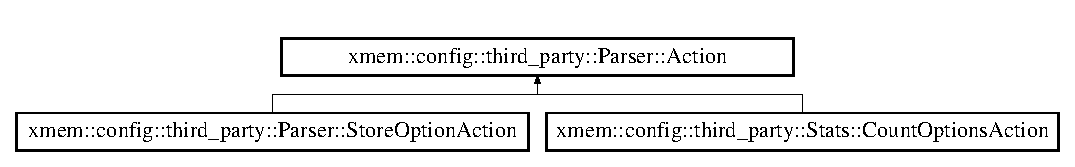
\includegraphics[height=1.794872cm]{structxmem_1_1config_1_1third__party_1_1_parser_1_1_action}
\end{center}
\end{figure}
\subsection*{Public Member Functions}
\begin{DoxyCompactItemize}
\item 
virtual bool \hyperlink{structxmem_1_1config_1_1third__party_1_1_parser_1_1_action_aeffc43365955b3dc5f54552093518aa5}{perform} (\hyperlink{classxmem_1_1config_1_1third__party_1_1_option}{Option} \&)
\begin{DoxyCompactList}\small\item\em Called by Parser\-::workhorse() for each \hyperlink{classxmem_1_1config_1_1third__party_1_1_option}{Option} that has been successfully parsed (including unknown options if they have a \hyperlink{structxmem_1_1config_1_1third__party_1_1_descriptor}{Descriptor} whose \hyperlink{structxmem_1_1config_1_1third__party_1_1_descriptor_a65b39f8d61de820bb5001d590e7dea5d}{Descriptor\-::check\-\_\-arg} does not return A\-R\-G\-\_\-\-I\-L\-L\-E\-G\-A\-L. \end{DoxyCompactList}\item 
virtual bool \hyperlink{structxmem_1_1config_1_1third__party_1_1_parser_1_1_action_a8f392f5dd42f483fa45ae5d83c9389ac}{finished} (int numargs, const char $\ast$$\ast$args)
\begin{DoxyCompactList}\small\item\em Called by Parser\-::workhorse() after finishing the parse. \end{DoxyCompactList}\end{DoxyCompactItemize}


\subsection{Member Function Documentation}
\hypertarget{structxmem_1_1config_1_1third__party_1_1_parser_1_1_action_a8f392f5dd42f483fa45ae5d83c9389ac}{\index{xmem\-::config\-::third\-\_\-party\-::\-Parser\-::\-Action@{xmem\-::config\-::third\-\_\-party\-::\-Parser\-::\-Action}!finished@{finished}}
\index{finished@{finished}!xmem::config::third_party::Parser::Action@{xmem\-::config\-::third\-\_\-party\-::\-Parser\-::\-Action}}
\subsubsection[{finished}]{\setlength{\rightskip}{0pt plus 5cm}virtual bool xmem\-::config\-::third\-\_\-party\-::\-Parser\-::\-Action\-::finished (
\begin{DoxyParamCaption}
\item[{int}]{numargs, }
\item[{const char $\ast$$\ast$}]{args}
\end{DoxyParamCaption}
)\hspace{0.3cm}{\ttfamily [inline]}, {\ttfamily [virtual]}}}\label{structxmem_1_1config_1_1third__party_1_1_parser_1_1_action_a8f392f5dd42f483fa45ae5d83c9389ac}


Called by Parser\-::workhorse() after finishing the parse. 


\begin{DoxyParams}{Parameters}
{\em numargs} & the number of non-\/option arguments remaining \\
\hline
{\em args} & pointer to the first remaining non-\/option argument (if numargs $>$ 0).\\
\hline
\end{DoxyParams}
\begin{DoxyReturn}{Returns}
{\ttfamily false} iff a fatal error has occurred. 
\end{DoxyReturn}


Reimplemented in \hyperlink{classxmem_1_1config_1_1third__party_1_1_parser_1_1_store_option_action_ad4e098cce0b0f97f025aec65d6226dff}{xmem\-::config\-::third\-\_\-party\-::\-Parser\-::\-Store\-Option\-Action}.

\hypertarget{structxmem_1_1config_1_1third__party_1_1_parser_1_1_action_aeffc43365955b3dc5f54552093518aa5}{\index{xmem\-::config\-::third\-\_\-party\-::\-Parser\-::\-Action@{xmem\-::config\-::third\-\_\-party\-::\-Parser\-::\-Action}!perform@{perform}}
\index{perform@{perform}!xmem::config::third_party::Parser::Action@{xmem\-::config\-::third\-\_\-party\-::\-Parser\-::\-Action}}
\subsubsection[{perform}]{\setlength{\rightskip}{0pt plus 5cm}virtual bool xmem\-::config\-::third\-\_\-party\-::\-Parser\-::\-Action\-::perform (
\begin{DoxyParamCaption}
\item[{{\bf Option} \&}]{}
\end{DoxyParamCaption}
)\hspace{0.3cm}{\ttfamily [inline]}, {\ttfamily [virtual]}}}\label{structxmem_1_1config_1_1third__party_1_1_parser_1_1_action_aeffc43365955b3dc5f54552093518aa5}


Called by Parser\-::workhorse() for each \hyperlink{classxmem_1_1config_1_1third__party_1_1_option}{Option} that has been successfully parsed (including unknown options if they have a \hyperlink{structxmem_1_1config_1_1third__party_1_1_descriptor}{Descriptor} whose \hyperlink{structxmem_1_1config_1_1third__party_1_1_descriptor_a65b39f8d61de820bb5001d590e7dea5d}{Descriptor\-::check\-\_\-arg} does not return A\-R\-G\-\_\-\-I\-L\-L\-E\-G\-A\-L. 

Returns {\ttfamily false} iff a fatal error has occured and the parse should be aborted. 

Reimplemented in \hyperlink{classxmem_1_1config_1_1third__party_1_1_parser_1_1_store_option_action_ab34c68452366b58ad4163602cf5f435d}{xmem\-::config\-::third\-\_\-party\-::\-Parser\-::\-Store\-Option\-Action}, and \hyperlink{classxmem_1_1config_1_1third__party_1_1_stats_1_1_count_options_action_aeacb83b2ed1520519dbfd678ac53b144}{xmem\-::config\-::third\-\_\-party\-::\-Stats\-::\-Count\-Options\-Action}.



The documentation for this struct was generated from the following file\-:\begin{DoxyCompactItemize}
\item 
src/include/\hyperlink{optionparser_8h}{optionparser.\-h}\end{DoxyCompactItemize}

\hypertarget{structxmem_1_1config_1_1third__party_1_1_arg}{}\section{xmem\+:\+:config\+:\+:third\+\_\+party\+:\+:Arg Struct Reference}
\label{structxmem_1_1config_1_1third__party_1_1_arg}\index{xmem\+::config\+::third\+\_\+party\+::\+Arg@{xmem\+::config\+::third\+\_\+party\+::\+Arg}}


Functions for checking the validity of option arguments.  




{\ttfamily \#include $<$optionparser.\+h$>$}

Inheritance diagram for xmem\+:\+:config\+:\+:third\+\_\+party\+:\+:Arg\+:\begin{figure}[H]
\begin{center}
\leavevmode
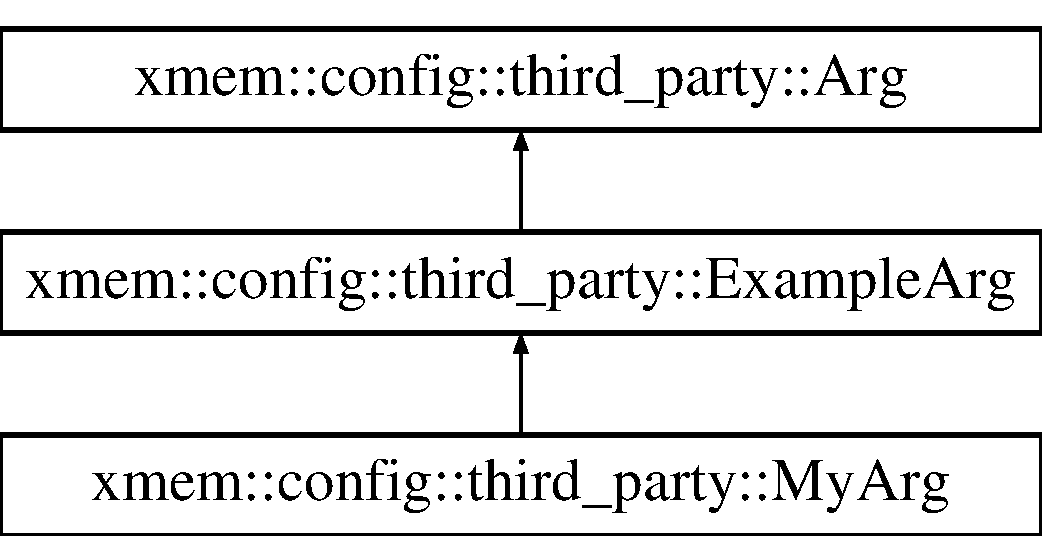
\includegraphics[height=3.000000cm]{structxmem_1_1config_1_1third__party_1_1_arg}
\end{center}
\end{figure}
\subsection*{Static Public Member Functions}
\begin{DoxyCompactItemize}
\item 
\hypertarget{structxmem_1_1config_1_1third__party_1_1_arg_afdfd4a0adea72c759ec04bf5feaf3ec0}{}static Arg\+Status \hyperlink{structxmem_1_1config_1_1third__party_1_1_arg_afdfd4a0adea72c759ec04bf5feaf3ec0}{None} (const \hyperlink{classxmem_1_1config_1_1third__party_1_1_option}{Option} \&, bool)\label{structxmem_1_1config_1_1third__party_1_1_arg_afdfd4a0adea72c759ec04bf5feaf3ec0}

\begin{DoxyCompactList}\small\item\em For options that don\textquotesingle{}t take an argument\+: Returns A\+R\+G\+\_\+\+N\+O\+N\+E. \end{DoxyCompactList}\item 
\hypertarget{structxmem_1_1config_1_1third__party_1_1_arg_a842eb05bf9c4581b082613f044691d89}{}static Arg\+Status \hyperlink{structxmem_1_1config_1_1third__party_1_1_arg_a842eb05bf9c4581b082613f044691d89}{Optional} (const \hyperlink{classxmem_1_1config_1_1third__party_1_1_option}{Option} \&option, bool)\label{structxmem_1_1config_1_1third__party_1_1_arg_a842eb05bf9c4581b082613f044691d89}

\begin{DoxyCompactList}\small\item\em Returns A\+R\+G\+\_\+\+O\+K if the argument is attached and A\+R\+G\+\_\+\+I\+G\+N\+O\+R\+E otherwise. \end{DoxyCompactList}\end{DoxyCompactItemize}


\subsection{Detailed Description}
Functions for checking the validity of option arguments. 

The following example code can serve as starting place for writing your own more complex Check\+Arg functions\+: 
\begin{DoxyCode}
\textcolor{keyword}{struct }Arg: \textcolor{keyword}{public} option::Arg
\{
  \textcolor{keyword}{static} \textcolor{keywordtype}{void} printError(\textcolor{keyword}{const} \textcolor{keywordtype}{char}* msg1, \textcolor{keyword}{const} option::Option& opt, \textcolor{keyword}{const} \textcolor{keywordtype}{char}* msg2)
  \{
    fprintf(stderr, \textcolor{stringliteral}{"ERROR: %s"}, msg1);
    fwrite(opt.name, opt.namelen, 1, stderr);
    fprintf(stderr, \textcolor{stringliteral}{"%s"}, msg2);
  \}

  \textcolor{keyword}{static} option::ArgStatus Unknown(\textcolor{keyword}{const} option::Option& option, \textcolor{keywordtype}{bool} msg)
  \{
    \textcolor{keywordflow}{if} (msg) printError(\textcolor{stringliteral}{"Unknown option '"}, option, \textcolor{stringliteral}{"'\(\backslash\)n"});
    \textcolor{keywordflow}{return} option::ARG\_ILLEGAL;
  \}

  \textcolor{keyword}{static} option::ArgStatus Required(\textcolor{keyword}{const} option::Option& option, \textcolor{keywordtype}{bool} msg)
  \{
    \textcolor{keywordflow}{if} (option.arg != 0)
      \textcolor{keywordflow}{return} option::ARG\_OK;

    \textcolor{keywordflow}{if} (msg) printError(\textcolor{stringliteral}{"Option '"}, option, \textcolor{stringliteral}{"' requires an argument\(\backslash\)n"});
    \textcolor{keywordflow}{return} option::ARG\_ILLEGAL;
  \}

  \textcolor{keyword}{static} option::ArgStatus NonEmpty(\textcolor{keyword}{const} option::Option& option, \textcolor{keywordtype}{bool} msg)
  \{
    \textcolor{keywordflow}{if} (option.arg != 0 && option.arg[0] != 0)
      \textcolor{keywordflow}{return} option::ARG\_OK;

    \textcolor{keywordflow}{if} (msg) printError(\textcolor{stringliteral}{"Option '"}, option, \textcolor{stringliteral}{"' requires a non-empty argument\(\backslash\)n"});
    \textcolor{keywordflow}{return} option::ARG\_ILLEGAL;
  \}

  \textcolor{keyword}{static} option::ArgStatus Numeric(\textcolor{keyword}{const} option::Option& option, \textcolor{keywordtype}{bool} msg)
  \{
    \textcolor{keywordtype}{char}* endptr = 0;
    \textcolor{keywordflow}{if} (option.arg != 0 && strtol(option.arg, &endptr, 10))\{\};
    \textcolor{keywordflow}{if} (endptr != option.arg && *endptr == 0)
      \textcolor{keywordflow}{return} option::ARG\_OK;

    \textcolor{keywordflow}{if} (msg) printError(\textcolor{stringliteral}{"Option '"}, option, \textcolor{stringliteral}{"' requires a numeric argument\(\backslash\)n"});
    \textcolor{keywordflow}{return} option::ARG\_ILLEGAL;
  \}
\};
\end{DoxyCode}
 

The documentation for this struct was generated from the following file\+:\begin{DoxyCompactItemize}
\item 
src/config/third\+\_\+party/\hyperlink{optionparser_8h}{optionparser.\+h}\end{DoxyCompactItemize}

\hypertarget{classxmem_1_1benchmark_1_1_benchmark}{}\section{xmem\+:\+:benchmark\+:\+:Benchmark Class Reference}
\label{classxmem_1_1benchmark_1_1_benchmark}\index{xmem\+::benchmark\+::\+Benchmark@{xmem\+::benchmark\+::\+Benchmark}}


Flexible abstract class for any memory benchmark.  




{\ttfamily \#include $<$Benchmark.\+h$>$}

Inheritance diagram for xmem\+:\+:benchmark\+:\+:Benchmark\+:\begin{figure}[H]
\begin{center}
\leavevmode
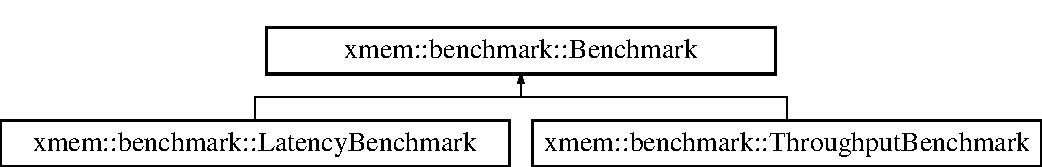
\includegraphics[height=2.000000cm]{classxmem_1_1benchmark_1_1_benchmark}
\end{center}
\end{figure}
\subsection*{Public Member Functions}
\begin{DoxyCompactItemize}
\item 
\hyperlink{classxmem_1_1benchmark_1_1_benchmark_a6eda9023866fc80e334d7d8d2a220817}{Benchmark} (void $\ast$mem\+\_\+array, size\+\_\+t len, uint32\+\_\+t iterations, xmem\+::common\+::chunk\+\_\+size\+\_\+t chunk\+\_\+size, uint32\+\_\+t cpu\+\_\+node, uint32\+\_\+t mem\+\_\+node, uint32\+\_\+t num\+\_\+worker\+\_\+threads, std\+::string name, \hyperlink{classxmem_1_1timers_1_1_timer}{xmem\+::timers\+::\+Timer} $\ast$timer, std\+::vector$<$ \hyperlink{classxmem_1_1power_1_1_power_reader}{xmem\+::power\+::\+Power\+Reader} $\ast$ $>$ dram\+\_\+power\+\_\+readers)
\begin{DoxyCompactList}\small\item\em Constructor. \end{DoxyCompactList}\item 
\hypertarget{classxmem_1_1benchmark_1_1_benchmark_a20476e07f09e2b20ed3e9a7f13a570e6}{}\hyperlink{classxmem_1_1benchmark_1_1_benchmark_a20476e07f09e2b20ed3e9a7f13a570e6}{$\sim$\+Benchmark} ()\label{classxmem_1_1benchmark_1_1_benchmark_a20476e07f09e2b20ed3e9a7f13a570e6}

\begin{DoxyCompactList}\small\item\em Destructor. \end{DoxyCompactList}\item 
virtual bool \hyperlink{classxmem_1_1benchmark_1_1_benchmark_aa0dbe60e525457770c835c6c72a0be6a}{run} ()=0
\begin{DoxyCompactList}\small\item\em Runs the benchmark. \end{DoxyCompactList}\item 
\hypertarget{classxmem_1_1benchmark_1_1_benchmark_ae788ccb9d65f543b1bc59f963ec5f2e2}{}virtual void \hyperlink{classxmem_1_1benchmark_1_1_benchmark_ae788ccb9d65f543b1bc59f963ec5f2e2}{report\+\_\+benchmark\+\_\+info} ()=0\label{classxmem_1_1benchmark_1_1_benchmark_ae788ccb9d65f543b1bc59f963ec5f2e2}

\begin{DoxyCompactList}\small\item\em Reports benchmark configuration details to the console. \end{DoxyCompactList}\item 
\hypertarget{classxmem_1_1benchmark_1_1_benchmark_ad9b74db44f972909dcba85dd32cef0a3}{}virtual void \hyperlink{classxmem_1_1benchmark_1_1_benchmark_ad9b74db44f972909dcba85dd32cef0a3}{report\+\_\+results} ()=0\label{classxmem_1_1benchmark_1_1_benchmark_ad9b74db44f972909dcba85dd32cef0a3}

\begin{DoxyCompactList}\small\item\em Reports results to the console. \end{DoxyCompactList}\item 
\hypertarget{classxmem_1_1benchmark_1_1_benchmark_a3cd60d59ac20e06f89cd3b4777bda5c7}{}void \hyperlink{classxmem_1_1benchmark_1_1_benchmark_a3cd60d59ac20e06f89cd3b4777bda5c7}{report\+\_\+power\+\_\+results} ()\label{classxmem_1_1benchmark_1_1_benchmark_a3cd60d59ac20e06f89cd3b4777bda5c7}

\begin{DoxyCompactList}\small\item\em Reports power measurement results to the console. \end{DoxyCompactList}\item 
bool \hyperlink{classxmem_1_1benchmark_1_1_benchmark_a5b08d817dd61666037957a3e23861512}{is\+Valid} ()
\begin{DoxyCompactList}\small\item\em Checks to see that the object is in a valid state. \end{DoxyCompactList}\item 
bool \hyperlink{classxmem_1_1benchmark_1_1_benchmark_a41afaa57de8ef2c66d31a41fa5f100c8}{has\+Run} ()
\begin{DoxyCompactList}\small\item\em Checks to see if the benchmark has run. \end{DoxyCompactList}\item 
double \hyperlink{classxmem_1_1benchmark_1_1_benchmark_a8bd36816a1414eaf488a6b63ba407200}{get\+Metric\+On\+Iter} (uint32\+\_\+t iter)
\begin{DoxyCompactList}\small\item\em Extracts the metric of interest for a given iteration. Units are interpreted by the inheriting class. \end{DoxyCompactList}\item 
double \hyperlink{classxmem_1_1benchmark_1_1_benchmark_a0beee3c5527e78ddb180ff20fe299e64}{get\+Average\+Metric} ()
\begin{DoxyCompactList}\small\item\em Gets the average benchmark metric across all iterations. \end{DoxyCompactList}\item 
double \hyperlink{classxmem_1_1benchmark_1_1_benchmark_aade8f8ba1268de6e112c222932b4224d}{get\+Average\+D\+R\+A\+M\+Power} (uint32\+\_\+t socket\+\_\+id)
\begin{DoxyCompactList}\small\item\em Gets the average D\+R\+A\+M power over the benchmark. \end{DoxyCompactList}\item 
double \hyperlink{classxmem_1_1benchmark_1_1_benchmark_a511908c2bd9bb5fa17d4b255a711636c}{get\+Peak\+D\+R\+A\+M\+Power} (uint32\+\_\+t socket\+\_\+id)
\begin{DoxyCompactList}\small\item\em Gets the peak D\+R\+A\+M power over the benchmark. \end{DoxyCompactList}\item 
size\+\_\+t \hyperlink{classxmem_1_1benchmark_1_1_benchmark_a3ca2577e4d2179710691c4aec7f93828}{get\+Len} ()
\begin{DoxyCompactList}\small\item\em Gets the length of the memory region in bytes. This is not necessarily the \char`\"{}working set size\char`\"{} depending on multithreading configuration. \end{DoxyCompactList}\item 
uint32\+\_\+t \hyperlink{classxmem_1_1benchmark_1_1_benchmark_a9fc7c775d0e29b22c8656e6e5bc10a48}{get\+Iterations} ()
\begin{DoxyCompactList}\small\item\em Gets the number of iterations for this benchmark. \end{DoxyCompactList}\item 
xmem\+::common\+::chunk\+\_\+size\+\_\+t \hyperlink{classxmem_1_1benchmark_1_1_benchmark_a434d6f97172982afdd16d3bde30e895f}{get\+Chunk\+Size} ()
\begin{DoxyCompactList}\small\item\em Gets the width of memory access used in this benchmark. \end{DoxyCompactList}\item 
uint32\+\_\+t \hyperlink{classxmem_1_1benchmark_1_1_benchmark_ad9e17919d6a8dd474495f3d7f0d05a29}{get\+C\+P\+U\+Node} ()
\begin{DoxyCompactList}\small\item\em Gets the C\+P\+U N\+U\+M\+A node used in this benchmark. \end{DoxyCompactList}\item 
uint32\+\_\+t \hyperlink{classxmem_1_1benchmark_1_1_benchmark_a35254c617874da5ccf8818692bdd0fe1}{get\+Mem\+Node} ()
\begin{DoxyCompactList}\small\item\em Gets the memory N\+U\+M\+A node used in this benchmark. \end{DoxyCompactList}\item 
uint32\+\_\+t \hyperlink{classxmem_1_1benchmark_1_1_benchmark_ad38e0629d25ae4177d4915f1aafd65f1}{get\+Num\+Threads} ()
\begin{DoxyCompactList}\small\item\em Gets the number of worker threads used in this benchmark. \end{DoxyCompactList}\item 
std\+::string \hyperlink{classxmem_1_1benchmark_1_1_benchmark_a18883dec146e768436c35946d40ab659}{get\+Name} ()
\begin{DoxyCompactList}\small\item\em Gets the human-\/friendly name of this benchmark. \end{DoxyCompactList}\end{DoxyCompactItemize}
\subsection*{Protected Member Functions}
\begin{DoxyCompactItemize}
\item 
bool \hyperlink{classxmem_1_1benchmark_1_1_benchmark_aaab5c124256e59540e061533323c64d7}{\+\_\+start\+\_\+power\+\_\+threads} ()
\begin{DoxyCompactList}\small\item\em Starts the D\+R\+A\+M power measurement threads. \end{DoxyCompactList}\item 
bool \hyperlink{classxmem_1_1benchmark_1_1_benchmark_a1c485c6f7fb6bbde588220d12129fa8e}{\+\_\+stop\+\_\+power\+\_\+threads} ()
\begin{DoxyCompactList}\small\item\em Stops the D\+R\+A\+M power measurement threads. This is a blocking call. \end{DoxyCompactList}\end{DoxyCompactItemize}
\subsection*{Protected Attributes}
\begin{DoxyCompactItemize}
\item 
void $\ast$ \hyperlink{classxmem_1_1benchmark_1_1_benchmark_a134705051be06902b276f5c21d435ed0}{\+\_\+mem\+\_\+array}
\item 
size\+\_\+t \hyperlink{classxmem_1_1benchmark_1_1_benchmark_ae97857f36cabdbe76eb00142835f7881}{\+\_\+len}
\item 
uint32\+\_\+t \hyperlink{classxmem_1_1benchmark_1_1_benchmark_a968403a473a3a4f713f4e73aa0757727}{\+\_\+iterations}
\item 
xmem\+::common\+::chunk\+\_\+size\+\_\+t \hyperlink{classxmem_1_1benchmark_1_1_benchmark_ae01156a2db05a6e3f7928a7433688f56}{\+\_\+chunk\+\_\+size}
\item 
size\+\_\+t $\ast$ \hyperlink{classxmem_1_1benchmark_1_1_benchmark_a1001cb321d8d655a71d435f5a06fdd3a}{\+\_\+indices}
\item 
uint32\+\_\+t \hyperlink{classxmem_1_1benchmark_1_1_benchmark_ab840cb1f53439eeeb6bdce7cd1eed78b}{\+\_\+cpu\+\_\+node}
\item 
uint32\+\_\+t \hyperlink{classxmem_1_1benchmark_1_1_benchmark_a8489553bc6539a9b19db72e9f6ca9a9e}{\+\_\+mem\+\_\+node}
\item 
uint32\+\_\+t \hyperlink{classxmem_1_1benchmark_1_1_benchmark_acb55cafc77a1b53ea9910d1be4306970}{\+\_\+num\+\_\+worker\+\_\+threads}
\item 
\hyperlink{classxmem_1_1timers_1_1_timer}{xmem\+::timers\+::\+Timer} $\ast$ \hyperlink{classxmem_1_1benchmark_1_1_benchmark_a673c700cb58ec0bc922f36d95dab12c9}{\+\_\+timer}
\item 
std\+::vector$<$ \hyperlink{classxmem_1_1power_1_1_power_reader}{xmem\+::power\+::\+Power\+Reader} $\ast$ $>$ \hyperlink{classxmem_1_1benchmark_1_1_benchmark_a6d4445364d9b6f17ec78be6c8cf253f1}{\+\_\+dram\+\_\+power\+\_\+readers}
\item 
std\+::vector$<$ \hyperlink{classxmem_1_1thread_1_1_thread}{xmem\+::thread\+::\+Thread} $\ast$ $>$ \hyperlink{classxmem_1_1benchmark_1_1_benchmark_a7aa95682a12f8fe4262b1fffb088d6ac}{\+\_\+dram\+\_\+power\+\_\+threads}
\item 
std\+::vector$<$ double $>$ \hyperlink{classxmem_1_1benchmark_1_1_benchmark_a179b20d5ac798c140650aa82e3658273}{\+\_\+average\+\_\+dram\+\_\+power\+\_\+socket}
\item 
std\+::vector$<$ double $>$ \hyperlink{classxmem_1_1benchmark_1_1_benchmark_a4da600693ba1df4fb69c1304b23b2cde}{\+\_\+peak\+\_\+dram\+\_\+power\+\_\+socket}
\item 
bool \hyperlink{classxmem_1_1benchmark_1_1_benchmark_a7caa584aa404d7751b781fd16c111fd0}{\+\_\+has\+Run}
\item 
std\+::vector$<$ double $>$ \hyperlink{classxmem_1_1benchmark_1_1_benchmark_a1c3ef60ba77f151cc4d5b4b77d2deefa}{\+\_\+metric\+On\+Iter}
\item 
double \hyperlink{classxmem_1_1benchmark_1_1_benchmark_a303386b7b243e39f2ca9a041ae819162}{\+\_\+average\+Metric}
\item 
std\+::string \hyperlink{classxmem_1_1benchmark_1_1_benchmark_ab9653ef73e0f1ca01e08286bdb35e4a6}{\+\_\+name}
\item 
bool \hyperlink{classxmem_1_1benchmark_1_1_benchmark_a87e133558776380738354191ec5e6560}{\+\_\+obj\+\_\+valid}
\item 
bool \hyperlink{classxmem_1_1benchmark_1_1_benchmark_af1a72e70f81c91f7c004ae01b2353288}{\+\_\+warning}
\end{DoxyCompactItemize}


\subsection{Detailed Description}
Flexible abstract class for any memory benchmark. 

This class provides a generic interface for interacting with a benchmark. All benchmarks should be derived from this class. 

\subsection{Constructor \& Destructor Documentation}
\hypertarget{classxmem_1_1benchmark_1_1_benchmark_a6eda9023866fc80e334d7d8d2a220817}{}\index{xmem\+::benchmark\+::\+Benchmark@{xmem\+::benchmark\+::\+Benchmark}!Benchmark@{Benchmark}}
\index{Benchmark@{Benchmark}!xmem\+::benchmark\+::\+Benchmark@{xmem\+::benchmark\+::\+Benchmark}}
\subsubsection[{Benchmark}]{\setlength{\rightskip}{0pt plus 5cm}Benchmark\+::\+Benchmark (
\begin{DoxyParamCaption}
\item[{void $\ast$}]{mem\+\_\+array, }
\item[{size\+\_\+t}]{len, }
\item[{uint32\+\_\+t}]{iterations, }
\item[{xmem\+::common\+::chunk\+\_\+size\+\_\+t}]{chunk\+\_\+size, }
\item[{uint32\+\_\+t}]{cpu\+\_\+node, }
\item[{uint32\+\_\+t}]{mem\+\_\+node, }
\item[{uint32\+\_\+t}]{num\+\_\+worker\+\_\+threads, }
\item[{std\+::string}]{name, }
\item[{{\bf xmem\+::timers\+::\+Timer} $\ast$}]{timer, }
\item[{std\+::vector$<$ {\bf xmem\+::power\+::\+Power\+Reader} $\ast$ $>$}]{dram\+\_\+power\+\_\+readers}
\end{DoxyParamCaption}
)}\label{classxmem_1_1benchmark_1_1_benchmark_a6eda9023866fc80e334d7d8d2a220817}


Constructor. 


\begin{DoxyParams}{Parameters}
{\em mem\+\_\+array} & a pointer to a contiguous chunk of memory that has been allocated for benchmarking among the worker threads. This should be aligned to a 256-\/bit boundary and should be the working set size times number of threads large. \\
\hline
{\em len} & Length of the raw\+\_\+mem\+\_\+array in bytes. This should be a multiple of 4 K\+B pages. \\
\hline
{\em iterations} & Number of iterations to do of the complete benchmark, to average out results. \\
\hline
{\em passes\+\_\+per\+\_\+iteration} & Number of passes to do in each iteration, to ensure timed section of code is \char`\"{}long enough\char`\"{}. \\
\hline
{\em chunk\+\_\+size} & encoded size of an individual memory access. \\
\hline
{\em cpu\+\_\+node} & the logical C\+P\+U N\+U\+M\+A node to use for the benchmark \\
\hline
{\em mem\+\_\+node} & the logical memory N\+U\+M\+A node used in the benchmark \\
\hline
{\em num\+\_\+worker\+\_\+threads} & number of worker threads to use in the benchmark \\
\hline
{\em name} & name of the benchmark to use when reporting \\
\hline
{\em timer} & pointer to an existing Timer \\
\hline
{\em dram\+\_\+power\+\_\+readers} & vector of pointers to Power\+Reader objects for measuring D\+R\+A\+M power \\
\hline
\end{DoxyParams}


\subsection{Member Function Documentation}
\hypertarget{classxmem_1_1benchmark_1_1_benchmark_aaab5c124256e59540e061533323c64d7}{}\index{xmem\+::benchmark\+::\+Benchmark@{xmem\+::benchmark\+::\+Benchmark}!\+\_\+start\+\_\+power\+\_\+threads@{\+\_\+start\+\_\+power\+\_\+threads}}
\index{\+\_\+start\+\_\+power\+\_\+threads@{\+\_\+start\+\_\+power\+\_\+threads}!xmem\+::benchmark\+::\+Benchmark@{xmem\+::benchmark\+::\+Benchmark}}
\subsubsection[{\+\_\+start\+\_\+power\+\_\+threads}]{\setlength{\rightskip}{0pt plus 5cm}bool Benchmark\+::\+\_\+start\+\_\+power\+\_\+threads (
\begin{DoxyParamCaption}
{}
\end{DoxyParamCaption}
)\hspace{0.3cm}{\ttfamily [protected]}}\label{classxmem_1_1benchmark_1_1_benchmark_aaab5c124256e59540e061533323c64d7}


Starts the D\+R\+A\+M power measurement threads. 

\begin{DoxyReturn}{Returns}
true on success 
\end{DoxyReturn}
\hypertarget{classxmem_1_1benchmark_1_1_benchmark_a1c485c6f7fb6bbde588220d12129fa8e}{}\index{xmem\+::benchmark\+::\+Benchmark@{xmem\+::benchmark\+::\+Benchmark}!\+\_\+stop\+\_\+power\+\_\+threads@{\+\_\+stop\+\_\+power\+\_\+threads}}
\index{\+\_\+stop\+\_\+power\+\_\+threads@{\+\_\+stop\+\_\+power\+\_\+threads}!xmem\+::benchmark\+::\+Benchmark@{xmem\+::benchmark\+::\+Benchmark}}
\subsubsection[{\+\_\+stop\+\_\+power\+\_\+threads}]{\setlength{\rightskip}{0pt plus 5cm}bool Benchmark\+::\+\_\+stop\+\_\+power\+\_\+threads (
\begin{DoxyParamCaption}
{}
\end{DoxyParamCaption}
)\hspace{0.3cm}{\ttfamily [protected]}}\label{classxmem_1_1benchmark_1_1_benchmark_a1c485c6f7fb6bbde588220d12129fa8e}


Stops the D\+R\+A\+M power measurement threads. This is a blocking call. 

\begin{DoxyReturn}{Returns}
true on success 
\end{DoxyReturn}
\hypertarget{classxmem_1_1benchmark_1_1_benchmark_aade8f8ba1268de6e112c222932b4224d}{}\index{xmem\+::benchmark\+::\+Benchmark@{xmem\+::benchmark\+::\+Benchmark}!get\+Average\+D\+R\+A\+M\+Power@{get\+Average\+D\+R\+A\+M\+Power}}
\index{get\+Average\+D\+R\+A\+M\+Power@{get\+Average\+D\+R\+A\+M\+Power}!xmem\+::benchmark\+::\+Benchmark@{xmem\+::benchmark\+::\+Benchmark}}
\subsubsection[{get\+Average\+D\+R\+A\+M\+Power}]{\setlength{\rightskip}{0pt plus 5cm}double Benchmark\+::get\+Average\+D\+R\+A\+M\+Power (
\begin{DoxyParamCaption}
\item[{uint32\+\_\+t}]{socket\+\_\+id}
\end{DoxyParamCaption}
)}\label{classxmem_1_1benchmark_1_1_benchmark_aade8f8ba1268de6e112c222932b4224d}


Gets the average D\+R\+A\+M power over the benchmark. 

\begin{DoxyReturn}{Returns}
The average D\+R\+A\+M power for a given socket in watts, or 0 if the data does not exist (power was unable to be collected or the benchmark has not run). 
\end{DoxyReturn}
\hypertarget{classxmem_1_1benchmark_1_1_benchmark_a0beee3c5527e78ddb180ff20fe299e64}{}\index{xmem\+::benchmark\+::\+Benchmark@{xmem\+::benchmark\+::\+Benchmark}!get\+Average\+Metric@{get\+Average\+Metric}}
\index{get\+Average\+Metric@{get\+Average\+Metric}!xmem\+::benchmark\+::\+Benchmark@{xmem\+::benchmark\+::\+Benchmark}}
\subsubsection[{get\+Average\+Metric}]{\setlength{\rightskip}{0pt plus 5cm}double Benchmark\+::get\+Average\+Metric (
\begin{DoxyParamCaption}
{}
\end{DoxyParamCaption}
)}\label{classxmem_1_1benchmark_1_1_benchmark_a0beee3c5527e78ddb180ff20fe299e64}


Gets the average benchmark metric across all iterations. 

\begin{DoxyReturn}{Returns}
The average metric. 
\end{DoxyReturn}
\hypertarget{classxmem_1_1benchmark_1_1_benchmark_a434d6f97172982afdd16d3bde30e895f}{}\index{xmem\+::benchmark\+::\+Benchmark@{xmem\+::benchmark\+::\+Benchmark}!get\+Chunk\+Size@{get\+Chunk\+Size}}
\index{get\+Chunk\+Size@{get\+Chunk\+Size}!xmem\+::benchmark\+::\+Benchmark@{xmem\+::benchmark\+::\+Benchmark}}
\subsubsection[{get\+Chunk\+Size}]{\setlength{\rightskip}{0pt plus 5cm}xmem\+::common\+::chunk\+\_\+size\+\_\+t Benchmark\+::get\+Chunk\+Size (
\begin{DoxyParamCaption}
{}
\end{DoxyParamCaption}
)}\label{classxmem_1_1benchmark_1_1_benchmark_a434d6f97172982afdd16d3bde30e895f}


Gets the width of memory access used in this benchmark. 

\begin{DoxyReturn}{Returns}
The chunk size for this benchmark. 
\end{DoxyReturn}
\hypertarget{classxmem_1_1benchmark_1_1_benchmark_ad9e17919d6a8dd474495f3d7f0d05a29}{}\index{xmem\+::benchmark\+::\+Benchmark@{xmem\+::benchmark\+::\+Benchmark}!get\+C\+P\+U\+Node@{get\+C\+P\+U\+Node}}
\index{get\+C\+P\+U\+Node@{get\+C\+P\+U\+Node}!xmem\+::benchmark\+::\+Benchmark@{xmem\+::benchmark\+::\+Benchmark}}
\subsubsection[{get\+C\+P\+U\+Node}]{\setlength{\rightskip}{0pt plus 5cm}uint32\+\_\+t Benchmark\+::get\+C\+P\+U\+Node (
\begin{DoxyParamCaption}
{}
\end{DoxyParamCaption}
)}\label{classxmem_1_1benchmark_1_1_benchmark_ad9e17919d6a8dd474495f3d7f0d05a29}


Gets the C\+P\+U N\+U\+M\+A node used in this benchmark. 

\begin{DoxyReturn}{Returns}
The N\+U\+M\+A C\+P\+U node used in this benchmark. 
\end{DoxyReturn}
\hypertarget{classxmem_1_1benchmark_1_1_benchmark_a9fc7c775d0e29b22c8656e6e5bc10a48}{}\index{xmem\+::benchmark\+::\+Benchmark@{xmem\+::benchmark\+::\+Benchmark}!get\+Iterations@{get\+Iterations}}
\index{get\+Iterations@{get\+Iterations}!xmem\+::benchmark\+::\+Benchmark@{xmem\+::benchmark\+::\+Benchmark}}
\subsubsection[{get\+Iterations}]{\setlength{\rightskip}{0pt plus 5cm}uint32\+\_\+t Benchmark\+::get\+Iterations (
\begin{DoxyParamCaption}
{}
\end{DoxyParamCaption}
)}\label{classxmem_1_1benchmark_1_1_benchmark_a9fc7c775d0e29b22c8656e6e5bc10a48}


Gets the number of iterations for this benchmark. 

\begin{DoxyReturn}{Returns}
The number of iterations for this benchmark. 
\end{DoxyReturn}
\hypertarget{classxmem_1_1benchmark_1_1_benchmark_a3ca2577e4d2179710691c4aec7f93828}{}\index{xmem\+::benchmark\+::\+Benchmark@{xmem\+::benchmark\+::\+Benchmark}!get\+Len@{get\+Len}}
\index{get\+Len@{get\+Len}!xmem\+::benchmark\+::\+Benchmark@{xmem\+::benchmark\+::\+Benchmark}}
\subsubsection[{get\+Len}]{\setlength{\rightskip}{0pt plus 5cm}size\+\_\+t Benchmark\+::get\+Len (
\begin{DoxyParamCaption}
{}
\end{DoxyParamCaption}
)}\label{classxmem_1_1benchmark_1_1_benchmark_a3ca2577e4d2179710691c4aec7f93828}


Gets the length of the memory region in bytes. This is not necessarily the \char`\"{}working set size\char`\"{} depending on multithreading configuration. 

\begin{DoxyReturn}{Returns}
Length of the memory region in bytes. 
\end{DoxyReturn}
\hypertarget{classxmem_1_1benchmark_1_1_benchmark_a35254c617874da5ccf8818692bdd0fe1}{}\index{xmem\+::benchmark\+::\+Benchmark@{xmem\+::benchmark\+::\+Benchmark}!get\+Mem\+Node@{get\+Mem\+Node}}
\index{get\+Mem\+Node@{get\+Mem\+Node}!xmem\+::benchmark\+::\+Benchmark@{xmem\+::benchmark\+::\+Benchmark}}
\subsubsection[{get\+Mem\+Node}]{\setlength{\rightskip}{0pt plus 5cm}uint32\+\_\+t Benchmark\+::get\+Mem\+Node (
\begin{DoxyParamCaption}
{}
\end{DoxyParamCaption}
)}\label{classxmem_1_1benchmark_1_1_benchmark_a35254c617874da5ccf8818692bdd0fe1}


Gets the memory N\+U\+M\+A node used in this benchmark. 

\begin{DoxyReturn}{Returns}
The N\+U\+M\+A memory node used in this benchmark. 
\end{DoxyReturn}
\hypertarget{classxmem_1_1benchmark_1_1_benchmark_a8bd36816a1414eaf488a6b63ba407200}{}\index{xmem\+::benchmark\+::\+Benchmark@{xmem\+::benchmark\+::\+Benchmark}!get\+Metric\+On\+Iter@{get\+Metric\+On\+Iter}}
\index{get\+Metric\+On\+Iter@{get\+Metric\+On\+Iter}!xmem\+::benchmark\+::\+Benchmark@{xmem\+::benchmark\+::\+Benchmark}}
\subsubsection[{get\+Metric\+On\+Iter}]{\setlength{\rightskip}{0pt plus 5cm}double Benchmark\+::get\+Metric\+On\+Iter (
\begin{DoxyParamCaption}
\item[{uint32\+\_\+t}]{iter}
\end{DoxyParamCaption}
)}\label{classxmem_1_1benchmark_1_1_benchmark_a8bd36816a1414eaf488a6b63ba407200}


Extracts the metric of interest for a given iteration. Units are interpreted by the inheriting class. 


\begin{DoxyParams}{Parameters}
{\em iter} & Iteration to extract. \\
\hline
\end{DoxyParams}
\begin{DoxyReturn}{Returns}
The metric on the iteration specified by the input. 
\end{DoxyReturn}
\hypertarget{classxmem_1_1benchmark_1_1_benchmark_a18883dec146e768436c35946d40ab659}{}\index{xmem\+::benchmark\+::\+Benchmark@{xmem\+::benchmark\+::\+Benchmark}!get\+Name@{get\+Name}}
\index{get\+Name@{get\+Name}!xmem\+::benchmark\+::\+Benchmark@{xmem\+::benchmark\+::\+Benchmark}}
\subsubsection[{get\+Name}]{\setlength{\rightskip}{0pt plus 5cm}std\+::string Benchmark\+::get\+Name (
\begin{DoxyParamCaption}
{}
\end{DoxyParamCaption}
)}\label{classxmem_1_1benchmark_1_1_benchmark_a18883dec146e768436c35946d40ab659}


Gets the human-\/friendly name of this benchmark. 

\begin{DoxyReturn}{Returns}
The benchmark test name. 
\end{DoxyReturn}
\hypertarget{classxmem_1_1benchmark_1_1_benchmark_ad38e0629d25ae4177d4915f1aafd65f1}{}\index{xmem\+::benchmark\+::\+Benchmark@{xmem\+::benchmark\+::\+Benchmark}!get\+Num\+Threads@{get\+Num\+Threads}}
\index{get\+Num\+Threads@{get\+Num\+Threads}!xmem\+::benchmark\+::\+Benchmark@{xmem\+::benchmark\+::\+Benchmark}}
\subsubsection[{get\+Num\+Threads}]{\setlength{\rightskip}{0pt plus 5cm}uint32\+\_\+t Benchmark\+::get\+Num\+Threads (
\begin{DoxyParamCaption}
{}
\end{DoxyParamCaption}
)}\label{classxmem_1_1benchmark_1_1_benchmark_ad38e0629d25ae4177d4915f1aafd65f1}


Gets the number of worker threads used in this benchmark. 

\begin{DoxyReturn}{Returns}
The number of worker threads used in this benchmark. 
\end{DoxyReturn}
\hypertarget{classxmem_1_1benchmark_1_1_benchmark_a511908c2bd9bb5fa17d4b255a711636c}{}\index{xmem\+::benchmark\+::\+Benchmark@{xmem\+::benchmark\+::\+Benchmark}!get\+Peak\+D\+R\+A\+M\+Power@{get\+Peak\+D\+R\+A\+M\+Power}}
\index{get\+Peak\+D\+R\+A\+M\+Power@{get\+Peak\+D\+R\+A\+M\+Power}!xmem\+::benchmark\+::\+Benchmark@{xmem\+::benchmark\+::\+Benchmark}}
\subsubsection[{get\+Peak\+D\+R\+A\+M\+Power}]{\setlength{\rightskip}{0pt plus 5cm}double Benchmark\+::get\+Peak\+D\+R\+A\+M\+Power (
\begin{DoxyParamCaption}
\item[{uint32\+\_\+t}]{socket\+\_\+id}
\end{DoxyParamCaption}
)}\label{classxmem_1_1benchmark_1_1_benchmark_a511908c2bd9bb5fa17d4b255a711636c}


Gets the peak D\+R\+A\+M power over the benchmark. 

\begin{DoxyReturn}{Returns}
The peak D\+R\+A\+M power for a given socket in watts, or 0 if the data does not exist (power was unable to be collected or the benchmark has not run). 
\end{DoxyReturn}
\hypertarget{classxmem_1_1benchmark_1_1_benchmark_a41afaa57de8ef2c66d31a41fa5f100c8}{}\index{xmem\+::benchmark\+::\+Benchmark@{xmem\+::benchmark\+::\+Benchmark}!has\+Run@{has\+Run}}
\index{has\+Run@{has\+Run}!xmem\+::benchmark\+::\+Benchmark@{xmem\+::benchmark\+::\+Benchmark}}
\subsubsection[{has\+Run}]{\setlength{\rightskip}{0pt plus 5cm}bool Benchmark\+::has\+Run (
\begin{DoxyParamCaption}
{}
\end{DoxyParamCaption}
)}\label{classxmem_1_1benchmark_1_1_benchmark_a41afaa57de8ef2c66d31a41fa5f100c8}


Checks to see if the benchmark has run. 

\begin{DoxyReturn}{Returns}
True if \hyperlink{classxmem_1_1benchmark_1_1_benchmark_aa0dbe60e525457770c835c6c72a0be6a}{run()} has already completed successfully. 
\end{DoxyReturn}
\hypertarget{classxmem_1_1benchmark_1_1_benchmark_a5b08d817dd61666037957a3e23861512}{}\index{xmem\+::benchmark\+::\+Benchmark@{xmem\+::benchmark\+::\+Benchmark}!is\+Valid@{is\+Valid}}
\index{is\+Valid@{is\+Valid}!xmem\+::benchmark\+::\+Benchmark@{xmem\+::benchmark\+::\+Benchmark}}
\subsubsection[{is\+Valid}]{\setlength{\rightskip}{0pt plus 5cm}bool Benchmark\+::is\+Valid (
\begin{DoxyParamCaption}
{}
\end{DoxyParamCaption}
)}\label{classxmem_1_1benchmark_1_1_benchmark_a5b08d817dd61666037957a3e23861512}


Checks to see that the object is in a valid state. 

\begin{DoxyReturn}{Returns}
True if the object was constructed correctly and can be used. 
\end{DoxyReturn}
\hypertarget{classxmem_1_1benchmark_1_1_benchmark_aa0dbe60e525457770c835c6c72a0be6a}{}\index{xmem\+::benchmark\+::\+Benchmark@{xmem\+::benchmark\+::\+Benchmark}!run@{run}}
\index{run@{run}!xmem\+::benchmark\+::\+Benchmark@{xmem\+::benchmark\+::\+Benchmark}}
\subsubsection[{run}]{\setlength{\rightskip}{0pt plus 5cm}virtual bool xmem\+::benchmark\+::\+Benchmark\+::run (
\begin{DoxyParamCaption}
{}
\end{DoxyParamCaption}
)\hspace{0.3cm}{\ttfamily [pure virtual]}}\label{classxmem_1_1benchmark_1_1_benchmark_aa0dbe60e525457770c835c6c72a0be6a}


Runs the benchmark. 

\begin{DoxyReturn}{Returns}
true on benchmark success 
\end{DoxyReturn}


Implemented in \hyperlink{classxmem_1_1benchmark_1_1_throughput_benchmark_a9f113e51d980830582148eb05c8810a3}{xmem\+::benchmark\+::\+Throughput\+Benchmark}, and \hyperlink{classxmem_1_1benchmark_1_1_latency_benchmark_ab68c299bf41fb30f9be597ff79188139}{xmem\+::benchmark\+::\+Latency\+Benchmark}.



\subsection{Member Data Documentation}
\hypertarget{classxmem_1_1benchmark_1_1_benchmark_a179b20d5ac798c140650aa82e3658273}{}\index{xmem\+::benchmark\+::\+Benchmark@{xmem\+::benchmark\+::\+Benchmark}!\+\_\+average\+\_\+dram\+\_\+power\+\_\+socket@{\+\_\+average\+\_\+dram\+\_\+power\+\_\+socket}}
\index{\+\_\+average\+\_\+dram\+\_\+power\+\_\+socket@{\+\_\+average\+\_\+dram\+\_\+power\+\_\+socket}!xmem\+::benchmark\+::\+Benchmark@{xmem\+::benchmark\+::\+Benchmark}}
\subsubsection[{\+\_\+average\+\_\+dram\+\_\+power\+\_\+socket}]{\setlength{\rightskip}{0pt plus 5cm}std\+::vector$<$double$>$ xmem\+::benchmark\+::\+Benchmark\+::\+\_\+average\+\_\+dram\+\_\+power\+\_\+socket\hspace{0.3cm}{\ttfamily [protected]}}\label{classxmem_1_1benchmark_1_1_benchmark_a179b20d5ac798c140650aa82e3658273}
The average D\+R\+A\+M power in this benchmark, per socket. \hypertarget{classxmem_1_1benchmark_1_1_benchmark_a303386b7b243e39f2ca9a041ae819162}{}\index{xmem\+::benchmark\+::\+Benchmark@{xmem\+::benchmark\+::\+Benchmark}!\+\_\+average\+Metric@{\+\_\+average\+Metric}}
\index{\+\_\+average\+Metric@{\+\_\+average\+Metric}!xmem\+::benchmark\+::\+Benchmark@{xmem\+::benchmark\+::\+Benchmark}}
\subsubsection[{\+\_\+average\+Metric}]{\setlength{\rightskip}{0pt plus 5cm}double xmem\+::benchmark\+::\+Benchmark\+::\+\_\+average\+Metric\hspace{0.3cm}{\ttfamily [protected]}}\label{classxmem_1_1benchmark_1_1_benchmark_a303386b7b243e39f2ca9a041ae819162}
Average metric over all iterations. Unit-\/less because any benchmark can set this metric as needed. It is up to the descendant class to interpret units. \hypertarget{classxmem_1_1benchmark_1_1_benchmark_ae01156a2db05a6e3f7928a7433688f56}{}\index{xmem\+::benchmark\+::\+Benchmark@{xmem\+::benchmark\+::\+Benchmark}!\+\_\+chunk\+\_\+size@{\+\_\+chunk\+\_\+size}}
\index{\+\_\+chunk\+\_\+size@{\+\_\+chunk\+\_\+size}!xmem\+::benchmark\+::\+Benchmark@{xmem\+::benchmark\+::\+Benchmark}}
\subsubsection[{\+\_\+chunk\+\_\+size}]{\setlength{\rightskip}{0pt plus 5cm}xmem\+::common\+::chunk\+\_\+size\+\_\+t xmem\+::benchmark\+::\+Benchmark\+::\+\_\+chunk\+\_\+size\hspace{0.3cm}{\ttfamily [protected]}}\label{classxmem_1_1benchmark_1_1_benchmark_ae01156a2db05a6e3f7928a7433688f56}
Chunk size of memory accesses in this benchmark. T\+O\+D\+O\+: Move this to \hyperlink{_throughput_benchmark_8h}{Throughput\+Benchmark.\+h}, as it does not apply in all situations, e.\+g. in \hyperlink{classxmem_1_1benchmark_1_1_latency_benchmark}{Latency\+Benchmark}. \hypertarget{classxmem_1_1benchmark_1_1_benchmark_ab840cb1f53439eeeb6bdce7cd1eed78b}{}\index{xmem\+::benchmark\+::\+Benchmark@{xmem\+::benchmark\+::\+Benchmark}!\+\_\+cpu\+\_\+node@{\+\_\+cpu\+\_\+node}}
\index{\+\_\+cpu\+\_\+node@{\+\_\+cpu\+\_\+node}!xmem\+::benchmark\+::\+Benchmark@{xmem\+::benchmark\+::\+Benchmark}}
\subsubsection[{\+\_\+cpu\+\_\+node}]{\setlength{\rightskip}{0pt plus 5cm}uint32\+\_\+t xmem\+::benchmark\+::\+Benchmark\+::\+\_\+cpu\+\_\+node\hspace{0.3cm}{\ttfamily [protected]}}\label{classxmem_1_1benchmark_1_1_benchmark_ab840cb1f53439eeeb6bdce7cd1eed78b}
The C\+P\+U N\+U\+M\+A node used in this benchmark. \hypertarget{classxmem_1_1benchmark_1_1_benchmark_a6d4445364d9b6f17ec78be6c8cf253f1}{}\index{xmem\+::benchmark\+::\+Benchmark@{xmem\+::benchmark\+::\+Benchmark}!\+\_\+dram\+\_\+power\+\_\+readers@{\+\_\+dram\+\_\+power\+\_\+readers}}
\index{\+\_\+dram\+\_\+power\+\_\+readers@{\+\_\+dram\+\_\+power\+\_\+readers}!xmem\+::benchmark\+::\+Benchmark@{xmem\+::benchmark\+::\+Benchmark}}
\subsubsection[{\+\_\+dram\+\_\+power\+\_\+readers}]{\setlength{\rightskip}{0pt plus 5cm}std\+::vector$<${\bf xmem\+::power\+::\+Power\+Reader}$\ast$$>$ xmem\+::benchmark\+::\+Benchmark\+::\+\_\+dram\+\_\+power\+\_\+readers\hspace{0.3cm}{\ttfamily [protected]}}\label{classxmem_1_1benchmark_1_1_benchmark_a6d4445364d9b6f17ec78be6c8cf253f1}
The power reading objects for measuring D\+R\+A\+M power on a per-\/socket basis during the benchmark. \hypertarget{classxmem_1_1benchmark_1_1_benchmark_a7aa95682a12f8fe4262b1fffb088d6ac}{}\index{xmem\+::benchmark\+::\+Benchmark@{xmem\+::benchmark\+::\+Benchmark}!\+\_\+dram\+\_\+power\+\_\+threads@{\+\_\+dram\+\_\+power\+\_\+threads}}
\index{\+\_\+dram\+\_\+power\+\_\+threads@{\+\_\+dram\+\_\+power\+\_\+threads}!xmem\+::benchmark\+::\+Benchmark@{xmem\+::benchmark\+::\+Benchmark}}
\subsubsection[{\+\_\+dram\+\_\+power\+\_\+threads}]{\setlength{\rightskip}{0pt plus 5cm}std\+::vector$<${\bf xmem\+::thread\+::\+Thread}$\ast$$>$ xmem\+::benchmark\+::\+Benchmark\+::\+\_\+dram\+\_\+power\+\_\+threads\hspace{0.3cm}{\ttfamily [protected]}}\label{classxmem_1_1benchmark_1_1_benchmark_a7aa95682a12f8fe4262b1fffb088d6ac}
The power reading threads for measuring D\+R\+A\+M power on a per-\/socket basis during the benchmark. These work with the D\+R\+A\+M power readers. Although they are worker threads, they are not counted as the \char`\"{}official\char`\"{} benchmarking worker threads. \hypertarget{classxmem_1_1benchmark_1_1_benchmark_a7caa584aa404d7751b781fd16c111fd0}{}\index{xmem\+::benchmark\+::\+Benchmark@{xmem\+::benchmark\+::\+Benchmark}!\+\_\+has\+Run@{\+\_\+has\+Run}}
\index{\+\_\+has\+Run@{\+\_\+has\+Run}!xmem\+::benchmark\+::\+Benchmark@{xmem\+::benchmark\+::\+Benchmark}}
\subsubsection[{\+\_\+has\+Run}]{\setlength{\rightskip}{0pt plus 5cm}bool xmem\+::benchmark\+::\+Benchmark\+::\+\_\+has\+Run\hspace{0.3cm}{\ttfamily [protected]}}\label{classxmem_1_1benchmark_1_1_benchmark_a7caa584aa404d7751b781fd16c111fd0}
Indicates whether the benchmark has run. \hypertarget{classxmem_1_1benchmark_1_1_benchmark_a1001cb321d8d655a71d435f5a06fdd3a}{}\index{xmem\+::benchmark\+::\+Benchmark@{xmem\+::benchmark\+::\+Benchmark}!\+\_\+indices@{\+\_\+indices}}
\index{\+\_\+indices@{\+\_\+indices}!xmem\+::benchmark\+::\+Benchmark@{xmem\+::benchmark\+::\+Benchmark}}
\subsubsection[{\+\_\+indices}]{\setlength{\rightskip}{0pt plus 5cm}size\+\_\+t$\ast$ xmem\+::benchmark\+::\+Benchmark\+::\+\_\+indices\hspace{0.3cm}{\ttfamily [protected]}}\label{classxmem_1_1benchmark_1_1_benchmark_a1001cb321d8d655a71d435f5a06fdd3a}
Pointer to a list of indices. This is for indirect memory addressing. Currently unused. T\+O\+D\+O\+: Remove this entirely? \hypertarget{classxmem_1_1benchmark_1_1_benchmark_a968403a473a3a4f713f4e73aa0757727}{}\index{xmem\+::benchmark\+::\+Benchmark@{xmem\+::benchmark\+::\+Benchmark}!\+\_\+iterations@{\+\_\+iterations}}
\index{\+\_\+iterations@{\+\_\+iterations}!xmem\+::benchmark\+::\+Benchmark@{xmem\+::benchmark\+::\+Benchmark}}
\subsubsection[{\+\_\+iterations}]{\setlength{\rightskip}{0pt plus 5cm}uint32\+\_\+t xmem\+::benchmark\+::\+Benchmark\+::\+\_\+iterations\hspace{0.3cm}{\ttfamily [protected]}}\label{classxmem_1_1benchmark_1_1_benchmark_a968403a473a3a4f713f4e73aa0757727}
Number of iterations used in this benchmark. \hypertarget{classxmem_1_1benchmark_1_1_benchmark_ae97857f36cabdbe76eb00142835f7881}{}\index{xmem\+::benchmark\+::\+Benchmark@{xmem\+::benchmark\+::\+Benchmark}!\+\_\+len@{\+\_\+len}}
\index{\+\_\+len@{\+\_\+len}!xmem\+::benchmark\+::\+Benchmark@{xmem\+::benchmark\+::\+Benchmark}}
\subsubsection[{\+\_\+len}]{\setlength{\rightskip}{0pt plus 5cm}size\+\_\+t xmem\+::benchmark\+::\+Benchmark\+::\+\_\+len\hspace{0.3cm}{\ttfamily [protected]}}\label{classxmem_1_1benchmark_1_1_benchmark_ae97857f36cabdbe76eb00142835f7881}
Length of the memory region in bytes. This is not the working set size per thread! \hypertarget{classxmem_1_1benchmark_1_1_benchmark_a134705051be06902b276f5c21d435ed0}{}\index{xmem\+::benchmark\+::\+Benchmark@{xmem\+::benchmark\+::\+Benchmark}!\+\_\+mem\+\_\+array@{\+\_\+mem\+\_\+array}}
\index{\+\_\+mem\+\_\+array@{\+\_\+mem\+\_\+array}!xmem\+::benchmark\+::\+Benchmark@{xmem\+::benchmark\+::\+Benchmark}}
\subsubsection[{\+\_\+mem\+\_\+array}]{\setlength{\rightskip}{0pt plus 5cm}void$\ast$ xmem\+::benchmark\+::\+Benchmark\+::\+\_\+mem\+\_\+array\hspace{0.3cm}{\ttfamily [protected]}}\label{classxmem_1_1benchmark_1_1_benchmark_a134705051be06902b276f5c21d435ed0}
Pointer to the memory region to use in this benchmark. \hypertarget{classxmem_1_1benchmark_1_1_benchmark_a8489553bc6539a9b19db72e9f6ca9a9e}{}\index{xmem\+::benchmark\+::\+Benchmark@{xmem\+::benchmark\+::\+Benchmark}!\+\_\+mem\+\_\+node@{\+\_\+mem\+\_\+node}}
\index{\+\_\+mem\+\_\+node@{\+\_\+mem\+\_\+node}!xmem\+::benchmark\+::\+Benchmark@{xmem\+::benchmark\+::\+Benchmark}}
\subsubsection[{\+\_\+mem\+\_\+node}]{\setlength{\rightskip}{0pt plus 5cm}uint32\+\_\+t xmem\+::benchmark\+::\+Benchmark\+::\+\_\+mem\+\_\+node\hspace{0.3cm}{\ttfamily [protected]}}\label{classxmem_1_1benchmark_1_1_benchmark_a8489553bc6539a9b19db72e9f6ca9a9e}
The memory N\+U\+M\+A node used in this benchmark. \hypertarget{classxmem_1_1benchmark_1_1_benchmark_a1c3ef60ba77f151cc4d5b4b77d2deefa}{}\index{xmem\+::benchmark\+::\+Benchmark@{xmem\+::benchmark\+::\+Benchmark}!\+\_\+metric\+On\+Iter@{\+\_\+metric\+On\+Iter}}
\index{\+\_\+metric\+On\+Iter@{\+\_\+metric\+On\+Iter}!xmem\+::benchmark\+::\+Benchmark@{xmem\+::benchmark\+::\+Benchmark}}
\subsubsection[{\+\_\+metric\+On\+Iter}]{\setlength{\rightskip}{0pt plus 5cm}std\+::vector$<$double$>$ xmem\+::benchmark\+::\+Benchmark\+::\+\_\+metric\+On\+Iter\hspace{0.3cm}{\ttfamily [protected]}}\label{classxmem_1_1benchmark_1_1_benchmark_a1c3ef60ba77f151cc4d5b4b77d2deefa}
Metrics for each iteration of the benchmark. Unit-\/less because any benchmark can set this metric as needed. It is up to the descendant class to interpret units. \hypertarget{classxmem_1_1benchmark_1_1_benchmark_ab9653ef73e0f1ca01e08286bdb35e4a6}{}\index{xmem\+::benchmark\+::\+Benchmark@{xmem\+::benchmark\+::\+Benchmark}!\+\_\+name@{\+\_\+name}}
\index{\+\_\+name@{\+\_\+name}!xmem\+::benchmark\+::\+Benchmark@{xmem\+::benchmark\+::\+Benchmark}}
\subsubsection[{\+\_\+name}]{\setlength{\rightskip}{0pt plus 5cm}std\+::string xmem\+::benchmark\+::\+Benchmark\+::\+\_\+name\hspace{0.3cm}{\ttfamily [protected]}}\label{classxmem_1_1benchmark_1_1_benchmark_ab9653ef73e0f1ca01e08286bdb35e4a6}
Name of this benchmark. \hypertarget{classxmem_1_1benchmark_1_1_benchmark_acb55cafc77a1b53ea9910d1be4306970}{}\index{xmem\+::benchmark\+::\+Benchmark@{xmem\+::benchmark\+::\+Benchmark}!\+\_\+num\+\_\+worker\+\_\+threads@{\+\_\+num\+\_\+worker\+\_\+threads}}
\index{\+\_\+num\+\_\+worker\+\_\+threads@{\+\_\+num\+\_\+worker\+\_\+threads}!xmem\+::benchmark\+::\+Benchmark@{xmem\+::benchmark\+::\+Benchmark}}
\subsubsection[{\+\_\+num\+\_\+worker\+\_\+threads}]{\setlength{\rightskip}{0pt plus 5cm}uint32\+\_\+t xmem\+::benchmark\+::\+Benchmark\+::\+\_\+num\+\_\+worker\+\_\+threads\hspace{0.3cm}{\ttfamily [protected]}}\label{classxmem_1_1benchmark_1_1_benchmark_acb55cafc77a1b53ea9910d1be4306970}
The number of worker threads used in this benchmark. \hypertarget{classxmem_1_1benchmark_1_1_benchmark_a87e133558776380738354191ec5e6560}{}\index{xmem\+::benchmark\+::\+Benchmark@{xmem\+::benchmark\+::\+Benchmark}!\+\_\+obj\+\_\+valid@{\+\_\+obj\+\_\+valid}}
\index{\+\_\+obj\+\_\+valid@{\+\_\+obj\+\_\+valid}!xmem\+::benchmark\+::\+Benchmark@{xmem\+::benchmark\+::\+Benchmark}}
\subsubsection[{\+\_\+obj\+\_\+valid}]{\setlength{\rightskip}{0pt plus 5cm}bool xmem\+::benchmark\+::\+Benchmark\+::\+\_\+obj\+\_\+valid\hspace{0.3cm}{\ttfamily [protected]}}\label{classxmem_1_1benchmark_1_1_benchmark_a87e133558776380738354191ec5e6560}
Indicates whether this benchmark object is valid. \hypertarget{classxmem_1_1benchmark_1_1_benchmark_a4da600693ba1df4fb69c1304b23b2cde}{}\index{xmem\+::benchmark\+::\+Benchmark@{xmem\+::benchmark\+::\+Benchmark}!\+\_\+peak\+\_\+dram\+\_\+power\+\_\+socket@{\+\_\+peak\+\_\+dram\+\_\+power\+\_\+socket}}
\index{\+\_\+peak\+\_\+dram\+\_\+power\+\_\+socket@{\+\_\+peak\+\_\+dram\+\_\+power\+\_\+socket}!xmem\+::benchmark\+::\+Benchmark@{xmem\+::benchmark\+::\+Benchmark}}
\subsubsection[{\+\_\+peak\+\_\+dram\+\_\+power\+\_\+socket}]{\setlength{\rightskip}{0pt plus 5cm}std\+::vector$<$double$>$ xmem\+::benchmark\+::\+Benchmark\+::\+\_\+peak\+\_\+dram\+\_\+power\+\_\+socket\hspace{0.3cm}{\ttfamily [protected]}}\label{classxmem_1_1benchmark_1_1_benchmark_a4da600693ba1df4fb69c1304b23b2cde}
The peak D\+R\+A\+M power in this benchmark, per socket. \hypertarget{classxmem_1_1benchmark_1_1_benchmark_a673c700cb58ec0bc922f36d95dab12c9}{}\index{xmem\+::benchmark\+::\+Benchmark@{xmem\+::benchmark\+::\+Benchmark}!\+\_\+timer@{\+\_\+timer}}
\index{\+\_\+timer@{\+\_\+timer}!xmem\+::benchmark\+::\+Benchmark@{xmem\+::benchmark\+::\+Benchmark}}
\subsubsection[{\+\_\+timer}]{\setlength{\rightskip}{0pt plus 5cm}{\bf xmem\+::timers\+::\+Timer}$\ast$ xmem\+::benchmark\+::\+Benchmark\+::\+\_\+timer\hspace{0.3cm}{\ttfamily [protected]}}\label{classxmem_1_1benchmark_1_1_benchmark_a673c700cb58ec0bc922f36d95dab12c9}
The reference timer for this benchmark. T\+O\+D\+O\+: Remove this. It isn\textquotesingle{}t thread safe anyway, so workers don\textquotesingle{}t use it. \hypertarget{classxmem_1_1benchmark_1_1_benchmark_af1a72e70f81c91f7c004ae01b2353288}{}\index{xmem\+::benchmark\+::\+Benchmark@{xmem\+::benchmark\+::\+Benchmark}!\+\_\+warning@{\+\_\+warning}}
\index{\+\_\+warning@{\+\_\+warning}!xmem\+::benchmark\+::\+Benchmark@{xmem\+::benchmark\+::\+Benchmark}}
\subsubsection[{\+\_\+warning}]{\setlength{\rightskip}{0pt plus 5cm}bool xmem\+::benchmark\+::\+Benchmark\+::\+\_\+warning\hspace{0.3cm}{\ttfamily [protected]}}\label{classxmem_1_1benchmark_1_1_benchmark_af1a72e70f81c91f7c004ae01b2353288}
Indicates whether the benchmarks results might be clearly questionable/inaccurate/incorrect due to a variety of factors. 

The documentation for this class was generated from the following files\+:\begin{DoxyCompactItemize}
\item 
src/benchmark/\hyperlink{_benchmark_8h}{Benchmark.\+h}\item 
src/benchmark/\hyperlink{_benchmark_8cpp}{Benchmark.\+cpp}\end{DoxyCompactItemize}

\hypertarget{classxmem_1_1benchmark_1_1_benchmark_manager}{}\section{xmem\+:\+:benchmark\+:\+:Benchmark\+Manager Class Reference}
\label{classxmem_1_1benchmark_1_1_benchmark_manager}\index{xmem\+::benchmark\+::\+Benchmark\+Manager@{xmem\+::benchmark\+::\+Benchmark\+Manager}}


Manages running all benchmarks at a high level.  




{\ttfamily \#include $<$Benchmark\+Manager.\+h$>$}

\subsection*{Public Member Functions}
\begin{DoxyCompactItemize}
\item 
\hyperlink{classxmem_1_1benchmark_1_1_benchmark_manager_a1990c0e85b05764d7819b6903d495ee1}{Benchmark\+Manager} (size\+\_\+t working\+\_\+set\+\_\+size, uint32\+\_\+t iterations\+\_\+per\+\_\+benchmark, bool output\+\_\+to\+\_\+file, std\+::string results\+\_\+filename)
\begin{DoxyCompactList}\small\item\em Constructor. \end{DoxyCompactList}\item 
\hypertarget{classxmem_1_1benchmark_1_1_benchmark_manager_ab1540ca105b7e3c4f5fe96aeb59cc649}{}\hyperlink{classxmem_1_1benchmark_1_1_benchmark_manager_ab1540ca105b7e3c4f5fe96aeb59cc649}{$\sim$\+Benchmark\+Manager} ()\label{classxmem_1_1benchmark_1_1_benchmark_manager_ab1540ca105b7e3c4f5fe96aeb59cc649}

\begin{DoxyCompactList}\small\item\em Destructor. \end{DoxyCompactList}\item 
bool \hyperlink{classxmem_1_1benchmark_1_1_benchmark_manager_a7b7f4694586af20262d2f3ebe3750d86}{run\+All} ()
\begin{DoxyCompactList}\small\item\em Runs all possible benchmark configurations. \end{DoxyCompactList}\item 
bool \hyperlink{classxmem_1_1benchmark_1_1_benchmark_manager_a47b21d3d8a1e1be93e7efd35a3374b0c}{run\+Throughput\+Benchmarks} ()
\begin{DoxyCompactList}\small\item\em Runs the throughput benchmarks. \end{DoxyCompactList}\item 
bool \hyperlink{classxmem_1_1benchmark_1_1_benchmark_manager_ac515058049ec46df410e4e8e7d858019}{run\+Latency\+Benchmarks} ()
\begin{DoxyCompactList}\small\item\em Runs the latency benchmark. \end{DoxyCompactList}\end{DoxyCompactItemize}


\subsection{Detailed Description}
Manages running all benchmarks at a high level. 

\subsection{Constructor \& Destructor Documentation}
\hypertarget{classxmem_1_1benchmark_1_1_benchmark_manager_a1990c0e85b05764d7819b6903d495ee1}{}\index{xmem\+::benchmark\+::\+Benchmark\+Manager@{xmem\+::benchmark\+::\+Benchmark\+Manager}!Benchmark\+Manager@{Benchmark\+Manager}}
\index{Benchmark\+Manager@{Benchmark\+Manager}!xmem\+::benchmark\+::\+Benchmark\+Manager@{xmem\+::benchmark\+::\+Benchmark\+Manager}}
\subsubsection[{Benchmark\+Manager}]{\setlength{\rightskip}{0pt plus 5cm}Benchmark\+Manager\+::\+Benchmark\+Manager (
\begin{DoxyParamCaption}
\item[{size\+\_\+t}]{working\+\_\+set\+\_\+size, }
\item[{uint32\+\_\+t}]{iterations\+\_\+per\+\_\+benchmark, }
\item[{bool}]{output\+\_\+to\+\_\+file, }
\item[{std\+::string}]{results\+\_\+filename}
\end{DoxyParamCaption}
)}\label{classxmem_1_1benchmark_1_1_benchmark_manager_a1990c0e85b05764d7819b6903d495ee1}


Constructor. 


\begin{DoxyParams}{Parameters}
{\em working\+\_\+set\+\_\+size} & Total memory to test in bytes on each N\+U\+M\+A node. The \hyperlink{classxmem_1_1benchmark_1_1_benchmark_manager}{Benchmark\+Manager} will try to allocate them by itself. \\
\hline
{\em iterations\+\_\+per\+\_\+benchmark} & Number of passes to run for each individual benchmark. \\
\hline
{\em output\+\_\+to\+\_\+file} & If true, write to file specified by results\+\_\+filename. \\
\hline
{\em results\+\_\+filename} & Filename to write results to if output\+\_\+to\+\_\+file is true. \\
\hline
\end{DoxyParams}


\subsection{Member Function Documentation}
\hypertarget{classxmem_1_1benchmark_1_1_benchmark_manager_a7b7f4694586af20262d2f3ebe3750d86}{}\index{xmem\+::benchmark\+::\+Benchmark\+Manager@{xmem\+::benchmark\+::\+Benchmark\+Manager}!run\+All@{run\+All}}
\index{run\+All@{run\+All}!xmem\+::benchmark\+::\+Benchmark\+Manager@{xmem\+::benchmark\+::\+Benchmark\+Manager}}
\subsubsection[{run\+All}]{\setlength{\rightskip}{0pt plus 5cm}bool Benchmark\+Manager\+::run\+All (
\begin{DoxyParamCaption}
{}
\end{DoxyParamCaption}
)}\label{classxmem_1_1benchmark_1_1_benchmark_manager_a7b7f4694586af20262d2f3ebe3750d86}


Runs all possible benchmark configurations. 

\begin{DoxyReturn}{Returns}
True on success. 
\end{DoxyReturn}
\hypertarget{classxmem_1_1benchmark_1_1_benchmark_manager_ac515058049ec46df410e4e8e7d858019}{}\index{xmem\+::benchmark\+::\+Benchmark\+Manager@{xmem\+::benchmark\+::\+Benchmark\+Manager}!run\+Latency\+Benchmarks@{run\+Latency\+Benchmarks}}
\index{run\+Latency\+Benchmarks@{run\+Latency\+Benchmarks}!xmem\+::benchmark\+::\+Benchmark\+Manager@{xmem\+::benchmark\+::\+Benchmark\+Manager}}
\subsubsection[{run\+Latency\+Benchmarks}]{\setlength{\rightskip}{0pt plus 5cm}bool Benchmark\+Manager\+::run\+Latency\+Benchmarks (
\begin{DoxyParamCaption}
{}
\end{DoxyParamCaption}
)}\label{classxmem_1_1benchmark_1_1_benchmark_manager_ac515058049ec46df410e4e8e7d858019}


Runs the latency benchmark. 

\begin{DoxyReturn}{Returns}
True on benchmarking success. 
\end{DoxyReturn}
\hypertarget{classxmem_1_1benchmark_1_1_benchmark_manager_a47b21d3d8a1e1be93e7efd35a3374b0c}{}\index{xmem\+::benchmark\+::\+Benchmark\+Manager@{xmem\+::benchmark\+::\+Benchmark\+Manager}!run\+Throughput\+Benchmarks@{run\+Throughput\+Benchmarks}}
\index{run\+Throughput\+Benchmarks@{run\+Throughput\+Benchmarks}!xmem\+::benchmark\+::\+Benchmark\+Manager@{xmem\+::benchmark\+::\+Benchmark\+Manager}}
\subsubsection[{run\+Throughput\+Benchmarks}]{\setlength{\rightskip}{0pt plus 5cm}bool Benchmark\+Manager\+::run\+Throughput\+Benchmarks (
\begin{DoxyParamCaption}
{}
\end{DoxyParamCaption}
)}\label{classxmem_1_1benchmark_1_1_benchmark_manager_a47b21d3d8a1e1be93e7efd35a3374b0c}


Runs the throughput benchmarks. 

\begin{DoxyReturn}{Returns}
True on benchmarking success. 
\end{DoxyReturn}


The documentation for this class was generated from the following files\+:\begin{DoxyCompactItemize}
\item 
src/include/\hyperlink{_benchmark_manager_8h}{Benchmark\+Manager.\+h}\item 
src/\hyperlink{_benchmark_manager_8cpp}{Benchmark\+Manager.\+cpp}\end{DoxyCompactItemize}

\hypertarget{classxmem_1_1common_1_1win_1_1third__party_1_1_c_pdh_query_1_1_c_exception}{}\section{xmem\+:\+:common\+:\+:win\+:\+:third\+\_\+party\+:\+:C\+Pdh\+Query\+:\+:C\+Exception Class Reference}
\label{classxmem_1_1common_1_1win_1_1third__party_1_1_c_pdh_query_1_1_c_exception}\index{xmem\+::common\+::win\+::third\+\_\+party\+::\+C\+Pdh\+Query\+::\+C\+Exception@{xmem\+::common\+::win\+::third\+\_\+party\+::\+C\+Pdh\+Query\+::\+C\+Exception}}
\subsection*{Public Member Functions}
\begin{DoxyCompactItemize}
\item 
\hypertarget{classxmem_1_1common_1_1win_1_1third__party_1_1_c_pdh_query_1_1_c_exception_a9dfc0cf08b098d834f73c0b9bc09e747}{}{\bfseries C\+Exception} (std\+::tstring const \&error\+Msg)\label{classxmem_1_1common_1_1win_1_1third__party_1_1_c_pdh_query_1_1_c_exception_a9dfc0cf08b098d834f73c0b9bc09e747}

\item 
\hypertarget{classxmem_1_1common_1_1win_1_1third__party_1_1_c_pdh_query_1_1_c_exception_ac8c712fa04667506d4f362bba183a812}{}std\+::tstring {\bfseries What} () const \label{classxmem_1_1common_1_1win_1_1third__party_1_1_c_pdh_query_1_1_c_exception_ac8c712fa04667506d4f362bba183a812}

\end{DoxyCompactItemize}


The documentation for this class was generated from the following file\+:\begin{DoxyCompactItemize}
\item 
src/common/win/third\+\_\+party/\hyperlink{win___c_pdh_query_8h}{win\+\_\+\+C\+Pdh\+Query.\+h}\end{DoxyCompactItemize}

\hypertarget{classxmem_1_1config_1_1_configurator}{}\section{xmem\+:\+:config\+:\+:Configurator Class Reference}
\label{classxmem_1_1config_1_1_configurator}\index{xmem\+::config\+::\+Configurator@{xmem\+::config\+::\+Configurator}}


Handles all user input interpretation and generates the necessary flags for running benchmarks.  




{\ttfamily \#include $<$Configurator.\+h$>$}

\subsection*{Public Member Functions}
\begin{DoxyCompactItemize}
\item 
\hypertarget{classxmem_1_1config_1_1_configurator_a8ae41e8976253affae2b905cb7ca2389}{}\hyperlink{classxmem_1_1config_1_1_configurator_a8ae41e8976253affae2b905cb7ca2389}{Configurator} ()\label{classxmem_1_1config_1_1_configurator_a8ae41e8976253affae2b905cb7ca2389}

\begin{DoxyCompactList}\small\item\em Default constructor. A default configuration is set. You will want to run \hyperlink{classxmem_1_1config_1_1_configurator_acd25216c6c3db19dd68a5f2ec9b0a061}{configure\+From\+Input()} most likely. \end{DoxyCompactList}\item 
\hyperlink{classxmem_1_1config_1_1_configurator_ab687c798957f36943f2af563fd67f402}{Configurator} (bool run\+Latency, bool run\+Throughput, size\+\_\+t working\+\_\+set\+\_\+size, uint32\+\_\+t iterations\+\_\+per\+\_\+test, std\+::string filename, bool use\+\_\+output\+\_\+file)
\begin{DoxyCompactList}\small\item\em Specialized constructor for when you don\textquotesingle{}t want to get config from input, and you want to pass it in directly. \end{DoxyCompactList}\item 
int \hyperlink{classxmem_1_1config_1_1_configurator_acd25216c6c3db19dd68a5f2ec9b0a061}{configure\+From\+Input} (int argc, char $\ast$argv\mbox{[}$\,$\mbox{]})
\begin{DoxyCompactList}\small\item\em Configures the tool based on user\textquotesingle{}s command-\/line inputs. \end{DoxyCompactList}\item 
bool \hyperlink{classxmem_1_1config_1_1_configurator_abb15795a835f9d17205d442120b720a9}{latency\+Test\+Selected} ()
\begin{DoxyCompactList}\small\item\em Indicates if the latency test has been selected. \end{DoxyCompactList}\item 
bool \hyperlink{classxmem_1_1config_1_1_configurator_a21bfd5b3c29b32223ea59e08aebcfe8c}{throughput\+Test\+Selected} ()
\begin{DoxyCompactList}\small\item\em Indicates if the throughput test has been selected. \end{DoxyCompactList}\item 
size\+\_\+t \hyperlink{classxmem_1_1config_1_1_configurator_ad237760f0e0f76add3693bded410d749}{get\+Working\+Set\+Size} ()
\begin{DoxyCompactList}\small\item\em Gets the working set size in bytes for each worker thread, if applicable. \end{DoxyCompactList}\item 
uint32\+\_\+t \hyperlink{classxmem_1_1config_1_1_configurator_a0cae90ae39a85c42b884f59c983ddb98}{get\+Iterations\+Per\+Test} ()
\begin{DoxyCompactList}\small\item\em Gets the number of iterations that should be run of each benchmark. \end{DoxyCompactList}\item 
std\+::string \hyperlink{classxmem_1_1config_1_1_configurator_ad05eaa100414599543085778ca75ff64}{get\+Output\+Filename} ()
\begin{DoxyCompactList}\small\item\em Gets the output filename to use, if applicable. \end{DoxyCompactList}\item 
bool \hyperlink{classxmem_1_1config_1_1_configurator_a10a655ca8cea9e4d1f65e3f907a858a1}{use\+Output\+File} ()
\begin{DoxyCompactList}\small\item\em Determines whether to generate an output C\+S\+V file. \end{DoxyCompactList}\end{DoxyCompactItemize}


\subsection{Detailed Description}
Handles all user input interpretation and generates the necessary flags for running benchmarks. 

\subsection{Constructor \& Destructor Documentation}
\hypertarget{classxmem_1_1config_1_1_configurator_ab687c798957f36943f2af563fd67f402}{}\index{xmem\+::config\+::\+Configurator@{xmem\+::config\+::\+Configurator}!Configurator@{Configurator}}
\index{Configurator@{Configurator}!xmem\+::config\+::\+Configurator@{xmem\+::config\+::\+Configurator}}
\subsubsection[{Configurator}]{\setlength{\rightskip}{0pt plus 5cm}Configurator\+::\+Configurator (
\begin{DoxyParamCaption}
\item[{bool}]{run\+Latency, }
\item[{bool}]{run\+Throughput, }
\item[{size\+\_\+t}]{working\+\_\+set\+\_\+size, }
\item[{uint32\+\_\+t}]{iterations\+\_\+per\+\_\+test, }
\item[{std\+::string}]{filename, }
\item[{bool}]{use\+\_\+output\+\_\+file}
\end{DoxyParamCaption}
)}\label{classxmem_1_1config_1_1_configurator_ab687c798957f36943f2af563fd67f402}


Specialized constructor for when you don\textquotesingle{}t want to get config from input, and you want to pass it in directly. 


\begin{DoxyParams}{Parameters}
{\em run\+Latency} & Indicates latency benchmarks should be run. \\
\hline
{\em run\+Throughput} & Indicates throughput benchmarks should be run. \\
\hline
{\em working\+\_\+set\+\_\+size} & The total size of memory to test in all benchmarks, in bytes. This M\+U\+S\+T be a multiple of 4\+K\+B pages. \\
\hline
{\em iterations\+\_\+per\+\_\+test} & For each unique benchmark test, this is the number of times to repeat it. \\
\hline
{\em filename} & Output filename to use. \\
\hline
{\em use\+\_\+output\+\_\+file} & If true, use the provided output filename. \\
\hline
\end{DoxyParams}


\subsection{Member Function Documentation}
\hypertarget{classxmem_1_1config_1_1_configurator_acd25216c6c3db19dd68a5f2ec9b0a061}{}\index{xmem\+::config\+::\+Configurator@{xmem\+::config\+::\+Configurator}!configure\+From\+Input@{configure\+From\+Input}}
\index{configure\+From\+Input@{configure\+From\+Input}!xmem\+::config\+::\+Configurator@{xmem\+::config\+::\+Configurator}}
\subsubsection[{configure\+From\+Input}]{\setlength{\rightskip}{0pt plus 5cm}int Configurator\+::configure\+From\+Input (
\begin{DoxyParamCaption}
\item[{int}]{argc, }
\item[{char $\ast$}]{argv\mbox{[}$\,$\mbox{]}}
\end{DoxyParamCaption}
)}\label{classxmem_1_1config_1_1_configurator_acd25216c6c3db19dd68a5f2ec9b0a061}


Configures the tool based on user\textquotesingle{}s command-\/line inputs. 


\begin{DoxyParams}{Parameters}
{\em argc} & The argc from \hyperlink{main_8cpp_a0ddf1224851353fc92bfbff6f499fa97}{main()}. \\
\hline
{\em argv} & The argv from \hyperlink{main_8cpp_a0ddf1224851353fc92bfbff6f499fa97}{main()}. \\
\hline
\end{DoxyParams}
\begin{DoxyReturn}{Returns}
0 on success. 
\end{DoxyReturn}
\hypertarget{classxmem_1_1config_1_1_configurator_a0cae90ae39a85c42b884f59c983ddb98}{}\index{xmem\+::config\+::\+Configurator@{xmem\+::config\+::\+Configurator}!get\+Iterations\+Per\+Test@{get\+Iterations\+Per\+Test}}
\index{get\+Iterations\+Per\+Test@{get\+Iterations\+Per\+Test}!xmem\+::config\+::\+Configurator@{xmem\+::config\+::\+Configurator}}
\subsubsection[{get\+Iterations\+Per\+Test}]{\setlength{\rightskip}{0pt plus 5cm}uint32\+\_\+t xmem\+::config\+::\+Configurator\+::get\+Iterations\+Per\+Test (
\begin{DoxyParamCaption}
{}
\end{DoxyParamCaption}
)\hspace{0.3cm}{\ttfamily [inline]}}\label{classxmem_1_1config_1_1_configurator_a0cae90ae39a85c42b884f59c983ddb98}


Gets the number of iterations that should be run of each benchmark. 

\begin{DoxyReturn}{Returns}
The iterations for each test. 
\end{DoxyReturn}
\hypertarget{classxmem_1_1config_1_1_configurator_ad05eaa100414599543085778ca75ff64}{}\index{xmem\+::config\+::\+Configurator@{xmem\+::config\+::\+Configurator}!get\+Output\+Filename@{get\+Output\+Filename}}
\index{get\+Output\+Filename@{get\+Output\+Filename}!xmem\+::config\+::\+Configurator@{xmem\+::config\+::\+Configurator}}
\subsubsection[{get\+Output\+Filename}]{\setlength{\rightskip}{0pt plus 5cm}std\+::string xmem\+::config\+::\+Configurator\+::get\+Output\+Filename (
\begin{DoxyParamCaption}
{}
\end{DoxyParamCaption}
)\hspace{0.3cm}{\ttfamily [inline]}}\label{classxmem_1_1config_1_1_configurator_ad05eaa100414599543085778ca75ff64}


Gets the output filename to use, if applicable. 

\begin{DoxyReturn}{Returns}
The output filename to use if \hyperlink{classxmem_1_1config_1_1_configurator_a10a655ca8cea9e4d1f65e3f907a858a1}{use\+Output\+File()} returns true. Otherwise return value is \char`\"{}\char`\"{}. 
\end{DoxyReturn}
\hypertarget{classxmem_1_1config_1_1_configurator_ad237760f0e0f76add3693bded410d749}{}\index{xmem\+::config\+::\+Configurator@{xmem\+::config\+::\+Configurator}!get\+Working\+Set\+Size@{get\+Working\+Set\+Size}}
\index{get\+Working\+Set\+Size@{get\+Working\+Set\+Size}!xmem\+::config\+::\+Configurator@{xmem\+::config\+::\+Configurator}}
\subsubsection[{get\+Working\+Set\+Size}]{\setlength{\rightskip}{0pt plus 5cm}size\+\_\+t xmem\+::config\+::\+Configurator\+::get\+Working\+Set\+Size (
\begin{DoxyParamCaption}
{}
\end{DoxyParamCaption}
)\hspace{0.3cm}{\ttfamily [inline]}}\label{classxmem_1_1config_1_1_configurator_ad237760f0e0f76add3693bded410d749}


Gets the working set size in bytes for each worker thread, if applicable. 

\begin{DoxyReturn}{Returns}
The working set size in bytes. 
\end{DoxyReturn}
\hypertarget{classxmem_1_1config_1_1_configurator_abb15795a835f9d17205d442120b720a9}{}\index{xmem\+::config\+::\+Configurator@{xmem\+::config\+::\+Configurator}!latency\+Test\+Selected@{latency\+Test\+Selected}}
\index{latency\+Test\+Selected@{latency\+Test\+Selected}!xmem\+::config\+::\+Configurator@{xmem\+::config\+::\+Configurator}}
\subsubsection[{latency\+Test\+Selected}]{\setlength{\rightskip}{0pt plus 5cm}bool xmem\+::config\+::\+Configurator\+::latency\+Test\+Selected (
\begin{DoxyParamCaption}
{}
\end{DoxyParamCaption}
)\hspace{0.3cm}{\ttfamily [inline]}}\label{classxmem_1_1config_1_1_configurator_abb15795a835f9d17205d442120b720a9}


Indicates if the latency test has been selected. 

\begin{DoxyReturn}{Returns}
True if the latency test has been selected to run. 
\end{DoxyReturn}
\hypertarget{classxmem_1_1config_1_1_configurator_a21bfd5b3c29b32223ea59e08aebcfe8c}{}\index{xmem\+::config\+::\+Configurator@{xmem\+::config\+::\+Configurator}!throughput\+Test\+Selected@{throughput\+Test\+Selected}}
\index{throughput\+Test\+Selected@{throughput\+Test\+Selected}!xmem\+::config\+::\+Configurator@{xmem\+::config\+::\+Configurator}}
\subsubsection[{throughput\+Test\+Selected}]{\setlength{\rightskip}{0pt plus 5cm}bool xmem\+::config\+::\+Configurator\+::throughput\+Test\+Selected (
\begin{DoxyParamCaption}
{}
\end{DoxyParamCaption}
)\hspace{0.3cm}{\ttfamily [inline]}}\label{classxmem_1_1config_1_1_configurator_a21bfd5b3c29b32223ea59e08aebcfe8c}


Indicates if the throughput test has been selected. 

\begin{DoxyReturn}{Returns}
True if the throughput test has been selected to run. 
\end{DoxyReturn}
\hypertarget{classxmem_1_1config_1_1_configurator_a10a655ca8cea9e4d1f65e3f907a858a1}{}\index{xmem\+::config\+::\+Configurator@{xmem\+::config\+::\+Configurator}!use\+Output\+File@{use\+Output\+File}}
\index{use\+Output\+File@{use\+Output\+File}!xmem\+::config\+::\+Configurator@{xmem\+::config\+::\+Configurator}}
\subsubsection[{use\+Output\+File}]{\setlength{\rightskip}{0pt plus 5cm}bool xmem\+::config\+::\+Configurator\+::use\+Output\+File (
\begin{DoxyParamCaption}
{}
\end{DoxyParamCaption}
)\hspace{0.3cm}{\ttfamily [inline]}}\label{classxmem_1_1config_1_1_configurator_a10a655ca8cea9e4d1f65e3f907a858a1}


Determines whether to generate an output C\+S\+V file. 

\begin{DoxyReturn}{Returns}
True if an output file should be used. 
\end{DoxyReturn}


The documentation for this class was generated from the following files\+:\begin{DoxyCompactItemize}
\item 
src/include/\hyperlink{_configurator_8h}{Configurator.\+h}\item 
src/\hyperlink{_configurator_8cpp}{Configurator.\+cpp}\end{DoxyCompactItemize}

\hypertarget{classxmem_1_1config_1_1third__party_1_1_stats_1_1_count_options_action}{\section{xmem\-:\-:config\-:\-:third\-\_\-party\-:\-:Stats\-:\-:Count\-Options\-Action Class Reference}
\label{classxmem_1_1config_1_1third__party_1_1_stats_1_1_count_options_action}\index{xmem\-::config\-::third\-\_\-party\-::\-Stats\-::\-Count\-Options\-Action@{xmem\-::config\-::third\-\_\-party\-::\-Stats\-::\-Count\-Options\-Action}}
}
Inheritance diagram for xmem\-:\-:config\-:\-:third\-\_\-party\-:\-:Stats\-:\-:Count\-Options\-Action\-:\begin{figure}[H]
\begin{center}
\leavevmode
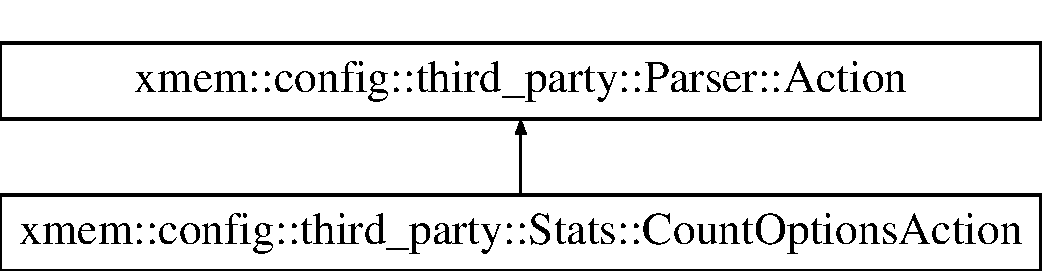
\includegraphics[height=2.000000cm]{classxmem_1_1config_1_1third__party_1_1_stats_1_1_count_options_action}
\end{center}
\end{figure}
\subsection*{Public Member Functions}
\begin{DoxyCompactItemize}
\item 
\hyperlink{classxmem_1_1config_1_1third__party_1_1_stats_1_1_count_options_action_ae3105daa0bee8d16e4fbe17e6306bd1a}{Count\-Options\-Action} (unsigned $\ast$buffer\-\_\-max\-\_\-)
\item 
bool \hyperlink{classxmem_1_1config_1_1third__party_1_1_stats_1_1_count_options_action_aeacb83b2ed1520519dbfd678ac53b144}{perform} (\hyperlink{classxmem_1_1config_1_1third__party_1_1_option}{Option} \&)
\begin{DoxyCompactList}\small\item\em Called by Parser\-::workhorse() for each \hyperlink{classxmem_1_1config_1_1third__party_1_1_option}{Option} that has been successfully parsed (including unknown options if they have a \hyperlink{structxmem_1_1config_1_1third__party_1_1_descriptor}{Descriptor} whose \hyperlink{structxmem_1_1config_1_1third__party_1_1_descriptor_a65b39f8d61de820bb5001d590e7dea5d}{Descriptor\-::check\-\_\-arg} does not return A\-R\-G\-\_\-\-I\-L\-L\-E\-G\-A\-L. \end{DoxyCompactList}\end{DoxyCompactItemize}


\subsection{Constructor \& Destructor Documentation}
\hypertarget{classxmem_1_1config_1_1third__party_1_1_stats_1_1_count_options_action_ae3105daa0bee8d16e4fbe17e6306bd1a}{\index{xmem\-::config\-::third\-\_\-party\-::\-Stats\-::\-Count\-Options\-Action@{xmem\-::config\-::third\-\_\-party\-::\-Stats\-::\-Count\-Options\-Action}!Count\-Options\-Action@{Count\-Options\-Action}}
\index{Count\-Options\-Action@{Count\-Options\-Action}!xmem::config::third_party::Stats::CountOptionsAction@{xmem\-::config\-::third\-\_\-party\-::\-Stats\-::\-Count\-Options\-Action}}
\subsubsection[{Count\-Options\-Action}]{\setlength{\rightskip}{0pt plus 5cm}xmem\-::config\-::third\-\_\-party\-::\-Stats\-::\-Count\-Options\-Action\-::\-Count\-Options\-Action (
\begin{DoxyParamCaption}
\item[{unsigned $\ast$}]{buffer\-\_\-max\-\_\-}
\end{DoxyParamCaption}
)\hspace{0.3cm}{\ttfamily [inline]}}}\label{classxmem_1_1config_1_1third__party_1_1_stats_1_1_count_options_action_ae3105daa0bee8d16e4fbe17e6306bd1a}
Creates a new \hyperlink{classxmem_1_1config_1_1third__party_1_1_stats_1_1_count_options_action}{Count\-Options\-Action} that will increase {\ttfamily $\ast$buffer\-\_\-max\-\_\-} for each parsed \hyperlink{classxmem_1_1config_1_1third__party_1_1_option}{Option}. 

\subsection{Member Function Documentation}
\hypertarget{classxmem_1_1config_1_1third__party_1_1_stats_1_1_count_options_action_aeacb83b2ed1520519dbfd678ac53b144}{\index{xmem\-::config\-::third\-\_\-party\-::\-Stats\-::\-Count\-Options\-Action@{xmem\-::config\-::third\-\_\-party\-::\-Stats\-::\-Count\-Options\-Action}!perform@{perform}}
\index{perform@{perform}!xmem::config::third_party::Stats::CountOptionsAction@{xmem\-::config\-::third\-\_\-party\-::\-Stats\-::\-Count\-Options\-Action}}
\subsubsection[{perform}]{\setlength{\rightskip}{0pt plus 5cm}bool xmem\-::config\-::third\-\_\-party\-::\-Stats\-::\-Count\-Options\-Action\-::perform (
\begin{DoxyParamCaption}
\item[{{\bf Option} \&}]{}
\end{DoxyParamCaption}
)\hspace{0.3cm}{\ttfamily [inline]}, {\ttfamily [virtual]}}}\label{classxmem_1_1config_1_1third__party_1_1_stats_1_1_count_options_action_aeacb83b2ed1520519dbfd678ac53b144}


Called by Parser\-::workhorse() for each \hyperlink{classxmem_1_1config_1_1third__party_1_1_option}{Option} that has been successfully parsed (including unknown options if they have a \hyperlink{structxmem_1_1config_1_1third__party_1_1_descriptor}{Descriptor} whose \hyperlink{structxmem_1_1config_1_1third__party_1_1_descriptor_a65b39f8d61de820bb5001d590e7dea5d}{Descriptor\-::check\-\_\-arg} does not return A\-R\-G\-\_\-\-I\-L\-L\-E\-G\-A\-L. 

Returns {\ttfamily false} iff a fatal error has occured and the parse should be aborted. 

Reimplemented from \hyperlink{structxmem_1_1config_1_1third__party_1_1_parser_1_1_action_aeffc43365955b3dc5f54552093518aa5}{xmem\-::config\-::third\-\_\-party\-::\-Parser\-::\-Action}.



The documentation for this class was generated from the following file\-:\begin{DoxyCompactItemize}
\item 
src/include/\hyperlink{optionparser_8h}{optionparser.\-h}\end{DoxyCompactItemize}

\hypertarget{classxmem_1_1common_1_1win_1_1third__party_1_1_c_pdh_query}{}\section{xmem\+:\+:common\+:\+:win\+:\+:third\+\_\+party\+:\+:C\+Pdh\+Query Class Reference}
\label{classxmem_1_1common_1_1win_1_1third__party_1_1_c_pdh_query}\index{xmem\+::common\+::win\+::third\+\_\+party\+::\+C\+Pdh\+Query@{xmem\+::common\+::win\+::third\+\_\+party\+::\+C\+Pdh\+Query}}


A third-\/party class for querying performance counter data from Windows.  




{\ttfamily \#include $<$win\+\_\+\+C\+Pdh\+Query.\+h$>$}

\subsection*{Classes}
\begin{DoxyCompactItemize}
\item 
class \hyperlink{classxmem_1_1common_1_1win_1_1third__party_1_1_c_pdh_query_1_1_c_exception}{C\+Exception}
\end{DoxyCompactItemize}
\subsection*{Public Member Functions}
\begin{DoxyCompactItemize}
\item 
\hypertarget{classxmem_1_1common_1_1win_1_1third__party_1_1_c_pdh_query_a9f68ac7575064085dc05bfdbf4e7b379}{}\hyperlink{classxmem_1_1common_1_1win_1_1third__party_1_1_c_pdh_query_a9f68ac7575064085dc05bfdbf4e7b379}{C\+Pdh\+Query} (std\+::tstring const \&counter\+Path)\label{classxmem_1_1common_1_1win_1_1third__party_1_1_c_pdh_query_a9f68ac7575064085dc05bfdbf4e7b379}

\begin{DoxyCompactList}\small\item\em Constructor. \end{DoxyCompactList}\item 
\hypertarget{classxmem_1_1common_1_1win_1_1third__party_1_1_c_pdh_query_adf839ba4df11e6544e95aafd004273b7}{}\hyperlink{classxmem_1_1common_1_1win_1_1third__party_1_1_c_pdh_query_adf839ba4df11e6544e95aafd004273b7}{$\sim$\+C\+Pdh\+Query} ()\label{classxmem_1_1common_1_1win_1_1third__party_1_1_c_pdh_query_adf839ba4df11e6544e95aafd004273b7}

\begin{DoxyCompactList}\small\item\em Destructor. The counter and query handle will be closed. \end{DoxyCompactList}\item 
\hypertarget{classxmem_1_1common_1_1win_1_1third__party_1_1_c_pdh_query_a529b4c7213b0d43cd7e5aeb0fe4dcb6b}{}std\+::map$<$ std\+::tstring, double $>$ \hyperlink{classxmem_1_1common_1_1win_1_1third__party_1_1_c_pdh_query_a529b4c7213b0d43cd7e5aeb0fe4dcb6b}{Collect\+Query\+Data} ()\label{classxmem_1_1common_1_1win_1_1third__party_1_1_c_pdh_query_a529b4c7213b0d43cd7e5aeb0fe4dcb6b}

\begin{DoxyCompactList}\small\item\em Collect all the data since the last sampling period. \end{DoxyCompactList}\end{DoxyCompactItemize}


\subsection{Detailed Description}
A third-\/party class for querying performance counter data from Windows. 

Source\+: \href{http://askldjd.wordpress.com/2011/01/05/a-pdh-helper-class-cpdhquery/,}{\tt http\+://askldjd.\+wordpress.\+com/2011/01/05/a-\/pdh-\/helper-\/class-\/cpdhquery/,} retrieved September 2014. Lightly modified and wrapped code to work here, like namespaces and some comments. \begin{DoxyAuthor}{Author}
Alan Ning 
\end{DoxyAuthor}


The documentation for this class was generated from the following file\+:\begin{DoxyCompactItemize}
\item 
src/common/win/third\+\_\+party/\hyperlink{win___c_pdh_query_8h}{win\+\_\+\+C\+Pdh\+Query.\+h}\end{DoxyCompactItemize}

\hypertarget{structxmem_1_1config_1_1third__party_1_1_descriptor}{\section{xmem\-:\-:config\-:\-:third\-\_\-party\-:\-:Descriptor Struct Reference}
\label{structxmem_1_1config_1_1third__party_1_1_descriptor}\index{xmem\-::config\-::third\-\_\-party\-::\-Descriptor@{xmem\-::config\-::third\-\_\-party\-::\-Descriptor}}
}


Describes an option, its help text (usage) and how it should be parsed.  




{\ttfamily \#include $<$optionparser.\-h$>$}

\subsection*{Public Attributes}
\begin{DoxyCompactItemize}
\item 
const unsigned \hyperlink{structxmem_1_1config_1_1third__party_1_1_descriptor_aacf3d44f35c61f22be65da078f60734b}{index}
\begin{DoxyCompactList}\small\item\em Index of this option's linked list in the array filled in by the parser. \end{DoxyCompactList}\item 
const int \hyperlink{structxmem_1_1config_1_1third__party_1_1_descriptor_a4b9e9a5c9b08ef575ea4f603c54bff63}{type}
\begin{DoxyCompactList}\small\item\em Used to distinguish between options with the same \hyperlink{structxmem_1_1config_1_1third__party_1_1_descriptor_aacf3d44f35c61f22be65da078f60734b}{index}. See \hyperlink{structxmem_1_1config_1_1third__party_1_1_descriptor_aacf3d44f35c61f22be65da078f60734b}{index} for details. \end{DoxyCompactList}\item 
const char $\ast$const \hyperlink{structxmem_1_1config_1_1third__party_1_1_descriptor_ac2dfb6bb8ca2f4aabf964a910cf0d59b}{shortopt}
\begin{DoxyCompactList}\small\item\em Each char in this string will be accepted as a short option character. \end{DoxyCompactList}\item 
const char $\ast$const \hyperlink{structxmem_1_1config_1_1third__party_1_1_descriptor_a7246a4bfc669f68bb406dece398be7bb}{longopt}
\begin{DoxyCompactList}\small\item\em The long option name (without the leading {\ttfamily --} ). \end{DoxyCompactList}\item 
const Check\-Arg \hyperlink{structxmem_1_1config_1_1third__party_1_1_descriptor_a65b39f8d61de820bb5001d590e7dea5d}{check\-\_\-arg}
\begin{DoxyCompactList}\small\item\em For each option that matches \hyperlink{structxmem_1_1config_1_1third__party_1_1_descriptor_ac2dfb6bb8ca2f4aabf964a910cf0d59b}{shortopt} or \hyperlink{structxmem_1_1config_1_1third__party_1_1_descriptor_a7246a4bfc669f68bb406dece398be7bb}{longopt} this function will be called to check a potential argument to the option. \end{DoxyCompactList}\item 
const char $\ast$ \hyperlink{structxmem_1_1config_1_1third__party_1_1_descriptor_a099340907003981132a053856dac0eaa}{help}
\begin{DoxyCompactList}\small\item\em The usage text associated with the options in this \hyperlink{structxmem_1_1config_1_1third__party_1_1_descriptor}{Descriptor}. \end{DoxyCompactList}\end{DoxyCompactItemize}


\subsection{Detailed Description}
Describes an option, its help text (usage) and how it should be parsed. 

The main input when constructing an option\-::\-Parser is an array of Descriptors.

\begin{DoxyParagraph}{Example\-:}

\begin{DoxyCode}
\textcolor{keyword}{enum} OptionIndex \{CREATE, ...\};
\textcolor{keyword}{enum} OptionType \{DISABLE, ENABLE, OTHER\};

\textcolor{keyword}{const} option::Descriptor usage[] = \{
  \{ CREATE,                                            \textcolor{comment}{// index}
    OTHER,                                             \textcolor{comment}{// type}
    \textcolor{stringliteral}{"c"},                                               \textcolor{comment}{// shortopt}
    \textcolor{stringliteral}{"create"},                                          \textcolor{comment}{// longopt}
    \hyperlink{structxmem_1_1config_1_1third__party_1_1_arg_afdfd4a0adea72c759ec04bf5feaf3ec0}{Arg::None},                                         \textcolor{comment}{// check\_arg}
    \textcolor{stringliteral}{"--create  Tells the program to create something."} \textcolor{comment}{// help}
  \}
  , ...
\};
\end{DoxyCode}
 
\end{DoxyParagraph}


\subsection{Member Data Documentation}
\hypertarget{structxmem_1_1config_1_1third__party_1_1_descriptor_a65b39f8d61de820bb5001d590e7dea5d}{\index{xmem\-::config\-::third\-\_\-party\-::\-Descriptor@{xmem\-::config\-::third\-\_\-party\-::\-Descriptor}!check\-\_\-arg@{check\-\_\-arg}}
\index{check\-\_\-arg@{check\-\_\-arg}!xmem::config::third_party::Descriptor@{xmem\-::config\-::third\-\_\-party\-::\-Descriptor}}
\subsubsection[{check\-\_\-arg}]{\setlength{\rightskip}{0pt plus 5cm}const Check\-Arg xmem\-::config\-::third\-\_\-party\-::\-Descriptor\-::check\-\_\-arg}}\label{structxmem_1_1config_1_1third__party_1_1_descriptor_a65b39f8d61de820bb5001d590e7dea5d}


For each option that matches \hyperlink{structxmem_1_1config_1_1third__party_1_1_descriptor_ac2dfb6bb8ca2f4aabf964a910cf0d59b}{shortopt} or \hyperlink{structxmem_1_1config_1_1third__party_1_1_descriptor_a7246a4bfc669f68bb406dece398be7bb}{longopt} this function will be called to check a potential argument to the option. 

This function will be called even if there is no potential argument. In that case it will be passed {\ttfamily N\-U\-L\-L} as {\ttfamily arg} parameter. Do not confuse this with the empty string.

See Check\-Arg for more information. \hypertarget{structxmem_1_1config_1_1third__party_1_1_descriptor_a099340907003981132a053856dac0eaa}{\index{xmem\-::config\-::third\-\_\-party\-::\-Descriptor@{xmem\-::config\-::third\-\_\-party\-::\-Descriptor}!help@{help}}
\index{help@{help}!xmem::config::third_party::Descriptor@{xmem\-::config\-::third\-\_\-party\-::\-Descriptor}}
\subsubsection[{help}]{\setlength{\rightskip}{0pt plus 5cm}const char$\ast$ xmem\-::config\-::third\-\_\-party\-::\-Descriptor\-::help}}\label{structxmem_1_1config_1_1third__party_1_1_descriptor_a099340907003981132a053856dac0eaa}


The usage text associated with the options in this \hyperlink{structxmem_1_1config_1_1third__party_1_1_descriptor}{Descriptor}. 

You can use option\-::print\-Usage() to format your usage message based on the {\ttfamily help} texts. You can use dummy Descriptors where \hyperlink{structxmem_1_1config_1_1third__party_1_1_descriptor_ac2dfb6bb8ca2f4aabf964a910cf0d59b}{shortopt} and \hyperlink{structxmem_1_1config_1_1third__party_1_1_descriptor_a7246a4bfc669f68bb406dece398be7bb}{longopt} are both the empty string to add text to the usage that is not related to a specific option.

See option\-::print\-Usage() for special formatting characters you can use in {\ttfamily help} to get a column layout.

\begin{DoxyAttention}{Attention}
Must be U\-T\-F-\/8-\/encoded. If your compiler supports C++11 you can use the \char`\"{}u8\char`\"{} prefix to make sure string literals are properly encoded. 
\end{DoxyAttention}
\hypertarget{structxmem_1_1config_1_1third__party_1_1_descriptor_aacf3d44f35c61f22be65da078f60734b}{\index{xmem\-::config\-::third\-\_\-party\-::\-Descriptor@{xmem\-::config\-::third\-\_\-party\-::\-Descriptor}!index@{index}}
\index{index@{index}!xmem::config::third_party::Descriptor@{xmem\-::config\-::third\-\_\-party\-::\-Descriptor}}
\subsubsection[{index}]{\setlength{\rightskip}{0pt plus 5cm}const unsigned xmem\-::config\-::third\-\_\-party\-::\-Descriptor\-::index}}\label{structxmem_1_1config_1_1third__party_1_1_descriptor_aacf3d44f35c61f22be65da078f60734b}


Index of this option's linked list in the array filled in by the parser. 

Command line options whose Descriptors have the same index will end up in the same linked list in the order in which they appear on the command line. If you have multiple long option aliases that refer to the same option, give their descriptors the same {\ttfamily index}.

If you have options that mean exactly opposite things (e.\-g. {\ttfamily --enable-\/foo} and {\ttfamily --disable-\/foo} ), you should also give them the same {\ttfamily index}, but distinguish them through different values for \hyperlink{structxmem_1_1config_1_1third__party_1_1_descriptor_a4b9e9a5c9b08ef575ea4f603c54bff63}{type}. That way they end up in the same list and you can just take the last element of the list and use its type. This way you get the usual behaviour where switches later on the command line override earlier ones without having to code it manually.

\begin{DoxyParagraph}{Tip\-:}
Use an enum rather than plain ints for better readability, as shown in the example at \hyperlink{structxmem_1_1config_1_1third__party_1_1_descriptor}{Descriptor}. 
\end{DoxyParagraph}
\hypertarget{structxmem_1_1config_1_1third__party_1_1_descriptor_a7246a4bfc669f68bb406dece398be7bb}{\index{xmem\-::config\-::third\-\_\-party\-::\-Descriptor@{xmem\-::config\-::third\-\_\-party\-::\-Descriptor}!longopt@{longopt}}
\index{longopt@{longopt}!xmem::config::third_party::Descriptor@{xmem\-::config\-::third\-\_\-party\-::\-Descriptor}}
\subsubsection[{longopt}]{\setlength{\rightskip}{0pt plus 5cm}const char$\ast$ const xmem\-::config\-::third\-\_\-party\-::\-Descriptor\-::longopt}}\label{structxmem_1_1config_1_1third__party_1_1_descriptor_a7246a4bfc669f68bb406dece398be7bb}


The long option name (without the leading {\ttfamily --} ). 

If this \hyperlink{structxmem_1_1config_1_1third__party_1_1_descriptor}{Descriptor} should not have a long option name, use the empty string \char`\"{}\char`\"{}. N\-U\-L\-L is not permitted here!

While \hyperlink{structxmem_1_1config_1_1third__party_1_1_descriptor_ac2dfb6bb8ca2f4aabf964a910cf0d59b}{shortopt} allows multiple short option characters, each \hyperlink{structxmem_1_1config_1_1third__party_1_1_descriptor}{Descriptor} can have only a single long option name. If you have multiple long option names referring to the same option use separate Descriptors that have the same \hyperlink{structxmem_1_1config_1_1third__party_1_1_descriptor_aacf3d44f35c61f22be65da078f60734b}{index} and \hyperlink{structxmem_1_1config_1_1third__party_1_1_descriptor_a4b9e9a5c9b08ef575ea4f603c54bff63}{type}. You may repeat short option characters in such an alias \hyperlink{structxmem_1_1config_1_1third__party_1_1_descriptor}{Descriptor} but there's no need to.

\begin{DoxyParagraph}{Dummy Descriptors\-:}
You can use dummy Descriptors with an empty string for both \hyperlink{structxmem_1_1config_1_1third__party_1_1_descriptor_ac2dfb6bb8ca2f4aabf964a910cf0d59b}{shortopt} and \hyperlink{structxmem_1_1config_1_1third__party_1_1_descriptor_a7246a4bfc669f68bb406dece398be7bb}{longopt} to add text to the usage that is not related to a specific option. See \hyperlink{structxmem_1_1config_1_1third__party_1_1_descriptor_a099340907003981132a053856dac0eaa}{help}. The first dummy \hyperlink{structxmem_1_1config_1_1third__party_1_1_descriptor}{Descriptor} will be used for unknown options (see below).
\end{DoxyParagraph}
\begin{DoxyParagraph}{Unknown Option Descriptor\-:}
The first dummy \hyperlink{structxmem_1_1config_1_1third__party_1_1_descriptor}{Descriptor} in the list of Descriptors, whose \hyperlink{structxmem_1_1config_1_1third__party_1_1_descriptor_ac2dfb6bb8ca2f4aabf964a910cf0d59b}{shortopt} and \hyperlink{structxmem_1_1config_1_1third__party_1_1_descriptor_a7246a4bfc669f68bb406dece398be7bb}{longopt} are both the empty string, will be used as the \hyperlink{structxmem_1_1config_1_1third__party_1_1_descriptor}{Descriptor} for unknown options. An unknown option is a string in the argument vector that is not a lone minus {\ttfamily '-\/'} but starts with a minus character and does not match any \hyperlink{structxmem_1_1config_1_1third__party_1_1_descriptor}{Descriptor}'s \hyperlink{structxmem_1_1config_1_1third__party_1_1_descriptor_ac2dfb6bb8ca2f4aabf964a910cf0d59b}{shortopt} or \hyperlink{structxmem_1_1config_1_1third__party_1_1_descriptor_a7246a4bfc669f68bb406dece398be7bb}{longopt}. \par
Note that the dummy descriptor's \hyperlink{structxmem_1_1config_1_1third__party_1_1_descriptor_a65b39f8d61de820bb5001d590e7dea5d}{check\-\_\-arg} function {\itshape will} be called and its return value will be evaluated as usual. I.\-e. if it returns A\-R\-G\-\_\-\-I\-L\-L\-E\-G\-A\-L the parsing will be aborted with {\ttfamily \hyperlink{classxmem_1_1config_1_1third__party_1_1_parser_a2c9fddb12fd9e4c735677e831afee138}{Parser\-::error()}==true}. \par
if {\ttfamily check\-\_\-arg} does not return A\-R\-G\-\_\-\-I\-L\-L\-E\-G\-A\-L the descriptor's \hyperlink{structxmem_1_1config_1_1third__party_1_1_descriptor_aacf3d44f35c61f22be65da078f60734b}{index} {\itshape will} be used to pick the linked list into which to put the unknown option. \par
If there is no dummy descriptor, unknown options will be dropped silently. 
\end{DoxyParagraph}
\hypertarget{structxmem_1_1config_1_1third__party_1_1_descriptor_ac2dfb6bb8ca2f4aabf964a910cf0d59b}{\index{xmem\-::config\-::third\-\_\-party\-::\-Descriptor@{xmem\-::config\-::third\-\_\-party\-::\-Descriptor}!shortopt@{shortopt}}
\index{shortopt@{shortopt}!xmem::config::third_party::Descriptor@{xmem\-::config\-::third\-\_\-party\-::\-Descriptor}}
\subsubsection[{shortopt}]{\setlength{\rightskip}{0pt plus 5cm}const char$\ast$ const xmem\-::config\-::third\-\_\-party\-::\-Descriptor\-::shortopt}}\label{structxmem_1_1config_1_1third__party_1_1_descriptor_ac2dfb6bb8ca2f4aabf964a910cf0d59b}


Each char in this string will be accepted as a short option character. 

The string must not include the minus character {\ttfamily '-\/'} or you'll get undefined behaviour.

If this \hyperlink{structxmem_1_1config_1_1third__party_1_1_descriptor}{Descriptor} should not have short option characters, use the empty string \char`\"{}\char`\"{}. N\-U\-L\-L is not permitted here!

See \hyperlink{structxmem_1_1config_1_1third__party_1_1_descriptor_a7246a4bfc669f68bb406dece398be7bb}{longopt} for more information. \hypertarget{structxmem_1_1config_1_1third__party_1_1_descriptor_a4b9e9a5c9b08ef575ea4f603c54bff63}{\index{xmem\-::config\-::third\-\_\-party\-::\-Descriptor@{xmem\-::config\-::third\-\_\-party\-::\-Descriptor}!type@{type}}
\index{type@{type}!xmem::config::third_party::Descriptor@{xmem\-::config\-::third\-\_\-party\-::\-Descriptor}}
\subsubsection[{type}]{\setlength{\rightskip}{0pt plus 5cm}const int xmem\-::config\-::third\-\_\-party\-::\-Descriptor\-::type}}\label{structxmem_1_1config_1_1third__party_1_1_descriptor_a4b9e9a5c9b08ef575ea4f603c54bff63}


Used to distinguish between options with the same \hyperlink{structxmem_1_1config_1_1third__party_1_1_descriptor_aacf3d44f35c61f22be65da078f60734b}{index}. See \hyperlink{structxmem_1_1config_1_1third__party_1_1_descriptor_aacf3d44f35c61f22be65da078f60734b}{index} for details. 

It is recommended that you use an enum rather than a plain int to make your code more readable. 

The documentation for this struct was generated from the following file\-:\begin{DoxyCompactItemize}
\item 
src/include/\hyperlink{optionparser_8h}{optionparser.\-h}\end{DoxyCompactItemize}

\hypertarget{classxmem_1_1config_1_1third__party_1_1_example_arg}{\section{xmem\-:\-:config\-:\-:third\-\_\-party\-:\-:Example\-Arg Class Reference}
\label{classxmem_1_1config_1_1third__party_1_1_example_arg}\index{xmem\-::config\-::third\-\_\-party\-::\-Example\-Arg@{xmem\-::config\-::third\-\_\-party\-::\-Example\-Arg}}
}
Inheritance diagram for xmem\-:\-:config\-:\-:third\-\_\-party\-:\-:Example\-Arg\-:\begin{figure}[H]
\begin{center}
\leavevmode
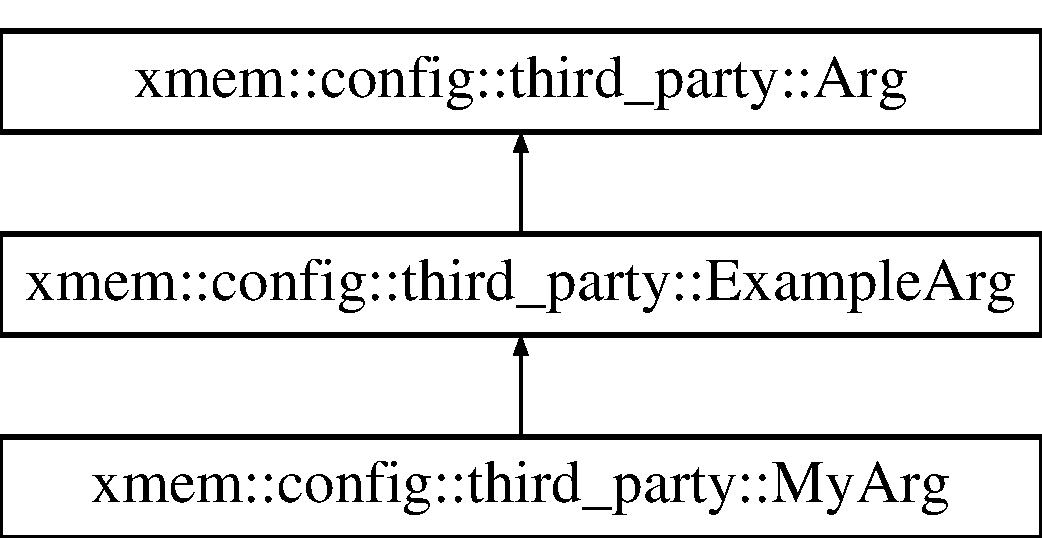
\includegraphics[height=3.000000cm]{classxmem_1_1config_1_1third__party_1_1_example_arg}
\end{center}
\end{figure}
\subsection*{Static Public Member Functions}
\begin{DoxyCompactItemize}
\item 
\hypertarget{classxmem_1_1config_1_1third__party_1_1_example_arg_a6121fd77d3727bb02ccd4438256beda0}{static void {\bfseries print\-Error} (const char $\ast$msg1, const \hyperlink{classxmem_1_1config_1_1third__party_1_1_option}{Option} \&opt, const char $\ast$msg2)}\label{classxmem_1_1config_1_1third__party_1_1_example_arg_a6121fd77d3727bb02ccd4438256beda0}

\item 
\hypertarget{classxmem_1_1config_1_1third__party_1_1_example_arg_a62f8121cadd8dfee722a1649caaa878c}{static Arg\-Status {\bfseries Unknown} (const \hyperlink{classxmem_1_1config_1_1third__party_1_1_option}{Option} \&option, bool msg)}\label{classxmem_1_1config_1_1third__party_1_1_example_arg_a62f8121cadd8dfee722a1649caaa878c}

\item 
\hypertarget{classxmem_1_1config_1_1third__party_1_1_example_arg_a9c71f36051376cdfbb807049a92921cf}{static Arg\-Status {\bfseries Required} (const \hyperlink{classxmem_1_1config_1_1third__party_1_1_option}{Option} \&option, bool msg)}\label{classxmem_1_1config_1_1third__party_1_1_example_arg_a9c71f36051376cdfbb807049a92921cf}

\item 
\hypertarget{classxmem_1_1config_1_1third__party_1_1_example_arg_ae641da2aeb27824f7a26b6859ba75dd3}{static Arg\-Status {\bfseries Non\-Empty} (const \hyperlink{classxmem_1_1config_1_1third__party_1_1_option}{Option} \&option, bool msg)}\label{classxmem_1_1config_1_1third__party_1_1_example_arg_ae641da2aeb27824f7a26b6859ba75dd3}

\end{DoxyCompactItemize}


The documentation for this class was generated from the following file\-:\begin{DoxyCompactItemize}
\item 
src/include/\hyperlink{_example_arg_8h}{Example\-Arg.\-h}\end{DoxyCompactItemize}

\hypertarget{structxmem_1_1config_1_1third__party_1_1_print_usage_implementation_1_1_function_writer}{\section{xmem\-:\-:config\-:\-:third\-\_\-party\-:\-:Print\-Usage\-Implementation\-:\-:Function\-Writer$<$ Function $>$ Struct Template Reference}
\label{structxmem_1_1config_1_1third__party_1_1_print_usage_implementation_1_1_function_writer}\index{xmem\-::config\-::third\-\_\-party\-::\-Print\-Usage\-Implementation\-::\-Function\-Writer$<$ Function $>$@{xmem\-::config\-::third\-\_\-party\-::\-Print\-Usage\-Implementation\-::\-Function\-Writer$<$ Function $>$}}
}
Inheritance diagram for xmem\-:\-:config\-:\-:third\-\_\-party\-:\-:Print\-Usage\-Implementation\-:\-:Function\-Writer$<$ Function $>$\-:\begin{figure}[H]
\begin{center}
\leavevmode
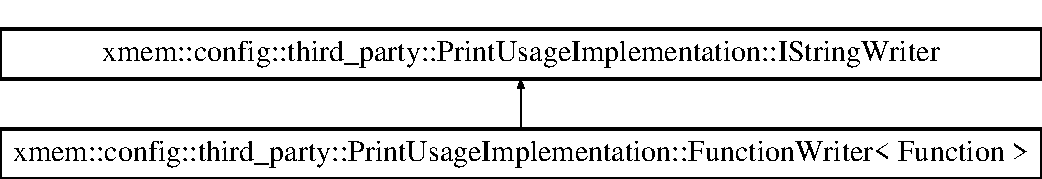
\includegraphics[height=2.000000cm]{structxmem_1_1config_1_1third__party_1_1_print_usage_implementation_1_1_function_writer}
\end{center}
\end{figure}
\subsection*{Public Member Functions}
\begin{DoxyCompactItemize}
\item 
\hypertarget{structxmem_1_1config_1_1third__party_1_1_print_usage_implementation_1_1_function_writer_abe1d90cb504d65f67564b73a4b49d9ee}{virtual void \hyperlink{structxmem_1_1config_1_1third__party_1_1_print_usage_implementation_1_1_function_writer_abe1d90cb504d65f67564b73a4b49d9ee}{operator()} (const char $\ast$str, int size)}\label{structxmem_1_1config_1_1third__party_1_1_print_usage_implementation_1_1_function_writer_abe1d90cb504d65f67564b73a4b49d9ee}

\begin{DoxyCompactList}\small\item\em Writes the given number of chars beginning at the given pointer somewhere. \end{DoxyCompactList}\item 
\hypertarget{structxmem_1_1config_1_1third__party_1_1_print_usage_implementation_1_1_function_writer_af078bf1e5f1545f343dd7111364c3936}{{\bfseries Function\-Writer} (Function $\ast$w)}\label{structxmem_1_1config_1_1third__party_1_1_print_usage_implementation_1_1_function_writer_af078bf1e5f1545f343dd7111364c3936}

\end{DoxyCompactItemize}
\subsection*{Public Attributes}
\begin{DoxyCompactItemize}
\item 
\hypertarget{structxmem_1_1config_1_1third__party_1_1_print_usage_implementation_1_1_function_writer_a15527210bafed3bf8accf1071a2ed710}{Function $\ast$ {\bfseries write}}\label{structxmem_1_1config_1_1third__party_1_1_print_usage_implementation_1_1_function_writer_a15527210bafed3bf8accf1071a2ed710}

\end{DoxyCompactItemize}


The documentation for this struct was generated from the following file\-:\begin{DoxyCompactItemize}
\item 
src/include/\hyperlink{optionparser_8h}{optionparser.\-h}\end{DoxyCompactItemize}

\hypertarget{structxmem_1_1config_1_1third__party_1_1_print_usage_implementation_1_1_i_string_writer}{\section{xmem\-:\-:config\-:\-:third\-\_\-party\-:\-:Print\-Usage\-Implementation\-:\-:I\-String\-Writer Struct Reference}
\label{structxmem_1_1config_1_1third__party_1_1_print_usage_implementation_1_1_i_string_writer}\index{xmem\-::config\-::third\-\_\-party\-::\-Print\-Usage\-Implementation\-::\-I\-String\-Writer@{xmem\-::config\-::third\-\_\-party\-::\-Print\-Usage\-Implementation\-::\-I\-String\-Writer}}
}
Inheritance diagram for xmem\-:\-:config\-:\-:third\-\_\-party\-:\-:Print\-Usage\-Implementation\-:\-:I\-String\-Writer\-:\begin{figure}[H]
\begin{center}
\leavevmode
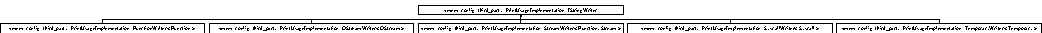
\includegraphics[height=0.440945cm]{structxmem_1_1config_1_1third__party_1_1_print_usage_implementation_1_1_i_string_writer}
\end{center}
\end{figure}
\subsection*{Public Member Functions}
\begin{DoxyCompactItemize}
\item 
\hypertarget{structxmem_1_1config_1_1third__party_1_1_print_usage_implementation_1_1_i_string_writer_aa391efef2dec3e18d614afb7e093a034}{virtual void \hyperlink{structxmem_1_1config_1_1third__party_1_1_print_usage_implementation_1_1_i_string_writer_aa391efef2dec3e18d614afb7e093a034}{operator()} (const char $\ast$, int)}\label{structxmem_1_1config_1_1third__party_1_1_print_usage_implementation_1_1_i_string_writer_aa391efef2dec3e18d614afb7e093a034}

\begin{DoxyCompactList}\small\item\em Writes the given number of chars beginning at the given pointer somewhere. \end{DoxyCompactList}\end{DoxyCompactItemize}


The documentation for this struct was generated from the following file\-:\begin{DoxyCompactItemize}
\item 
src/include/\hyperlink{optionparser_8h}{optionparser.\-h}\end{DoxyCompactItemize}

\hypertarget{classxmem_1_1benchmark_1_1_latency_benchmark}{}\section{xmem\+:\+:benchmark\+:\+:Latency\+Benchmark Class Reference}
\label{classxmem_1_1benchmark_1_1_latency_benchmark}\index{xmem\+::benchmark\+::\+Latency\+Benchmark@{xmem\+::benchmark\+::\+Latency\+Benchmark}}


A type of benchmark that measures memory latency via random pointer chasing. T\+O\+D\+O\+: loaded latency tests.  




{\ttfamily \#include $<$Latency\+Benchmark.\+h$>$}

Inheritance diagram for xmem\+:\+:benchmark\+:\+:Latency\+Benchmark\+:\begin{figure}[H]
\begin{center}
\leavevmode
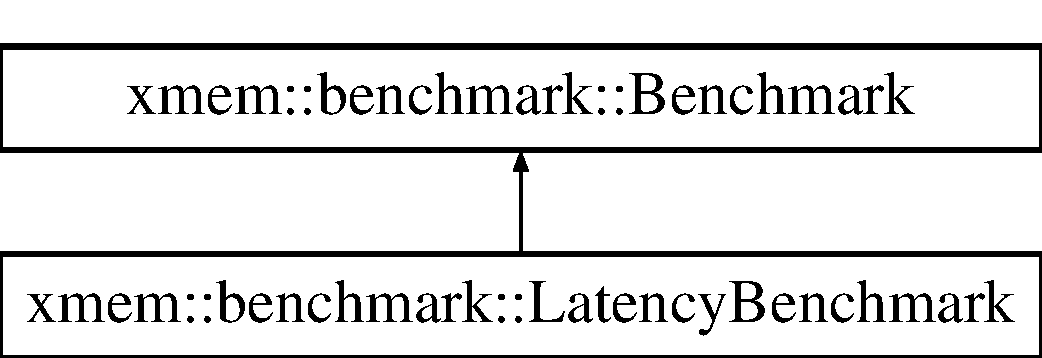
\includegraphics[height=2.000000cm]{classxmem_1_1benchmark_1_1_latency_benchmark}
\end{center}
\end{figure}
\subsection*{Public Types}
\begin{DoxyCompactItemize}
\item 
\hypertarget{classxmem_1_1benchmark_1_1_latency_benchmark_aac378764f476152456a39c9eb1e06c29}{}typedef int32\+\_\+t($\ast$ {\bfseries Latency\+Bench\+Function}) (uintptr\+\_\+t $\ast$, uintptr\+\_\+t $\ast$$\ast$, size\+\_\+t)\label{classxmem_1_1benchmark_1_1_latency_benchmark_aac378764f476152456a39c9eb1e06c29}

\end{DoxyCompactItemize}
\subsection*{Public Member Functions}
\begin{DoxyCompactItemize}
\item 
\hyperlink{classxmem_1_1benchmark_1_1_latency_benchmark_a485434e0f506427b28073a2a3e287e21}{Latency\+Benchmark} (void $\ast$mem\+\_\+array, size\+\_\+t len, uint32\+\_\+t iterations, uint32\+\_\+t cpu\+\_\+node, uint32\+\_\+t mem\+\_\+node, uint32\+\_\+t num\+\_\+worker\+\_\+threads, std\+::string name, \hyperlink{classxmem_1_1timers_1_1_timer}{xmem\+::timers\+::\+Timer} $\ast$timer, std\+::vector$<$ \hyperlink{classxmem_1_1power_1_1_power_reader}{xmem\+::power\+::\+Power\+Reader} $\ast$ $>$ dram\+\_\+power\+\_\+readers)
\item 
virtual bool \hyperlink{classxmem_1_1benchmark_1_1_latency_benchmark_ab68c299bf41fb30f9be597ff79188139}{run} ()
\begin{DoxyCompactList}\small\item\em Runs the benchmark. \end{DoxyCompactList}\item 
\hypertarget{classxmem_1_1benchmark_1_1_latency_benchmark_a2714dfbf9be2eef8ac4089ad610db651}{}virtual void \hyperlink{classxmem_1_1benchmark_1_1_latency_benchmark_a2714dfbf9be2eef8ac4089ad610db651}{report\+\_\+benchmark\+\_\+info} ()\label{classxmem_1_1benchmark_1_1_latency_benchmark_a2714dfbf9be2eef8ac4089ad610db651}

\begin{DoxyCompactList}\small\item\em Outputs the benchmark configuration to the console. \end{DoxyCompactList}\item 
\hypertarget{classxmem_1_1benchmark_1_1_latency_benchmark_ae16f89eb9f413734989ef8c51ec3e066}{}virtual void \hyperlink{classxmem_1_1benchmark_1_1_latency_benchmark_ae16f89eb9f413734989ef8c51ec3e066}{report\+\_\+results} ()\label{classxmem_1_1benchmark_1_1_latency_benchmark_ae16f89eb9f413734989ef8c51ec3e066}

\begin{DoxyCompactList}\small\item\em Outputs a report of the benchmark results to the console if \hyperlink{classxmem_1_1benchmark_1_1_latency_benchmark_ab68c299bf41fb30f9be597ff79188139}{run()} returned true. \end{DoxyCompactList}\end{DoxyCompactItemize}
\subsection*{Additional Inherited Members}


\subsection{Detailed Description}
A type of benchmark that measures memory latency via random pointer chasing. T\+O\+D\+O\+: loaded latency tests. 

\subsection{Constructor \& Destructor Documentation}
\hypertarget{classxmem_1_1benchmark_1_1_latency_benchmark_a485434e0f506427b28073a2a3e287e21}{}\index{xmem\+::benchmark\+::\+Latency\+Benchmark@{xmem\+::benchmark\+::\+Latency\+Benchmark}!Latency\+Benchmark@{Latency\+Benchmark}}
\index{Latency\+Benchmark@{Latency\+Benchmark}!xmem\+::benchmark\+::\+Latency\+Benchmark@{xmem\+::benchmark\+::\+Latency\+Benchmark}}
\subsubsection[{Latency\+Benchmark}]{\setlength{\rightskip}{0pt plus 5cm}Latency\+Benchmark\+::\+Latency\+Benchmark (
\begin{DoxyParamCaption}
\item[{void $\ast$}]{mem\+\_\+array, }
\item[{size\+\_\+t}]{len, }
\item[{uint32\+\_\+t}]{iterations, }
\item[{uint32\+\_\+t}]{cpu\+\_\+node, }
\item[{uint32\+\_\+t}]{mem\+\_\+node, }
\item[{uint32\+\_\+t}]{num\+\_\+worker\+\_\+threads, }
\item[{std\+::string}]{name, }
\item[{{\bf xmem\+::timers\+::\+Timer} $\ast$}]{timer, }
\item[{std\+::vector$<$ {\bf xmem\+::power\+::\+Power\+Reader} $\ast$ $>$}]{dram\+\_\+power\+\_\+readers}
\end{DoxyParamCaption}
)}\label{classxmem_1_1benchmark_1_1_latency_benchmark_a485434e0f506427b28073a2a3e287e21}
Constructor. 
\begin{DoxyParams}{Parameters}
{\em mem\+\_\+array} & a pointer to a contiguous chunk of memory that has been allocated for benchmarking among the worker threads. This should be aligned to a 256-\/bit boundary and should be the working set size times number of threads large. \\
\hline
{\em len} & Length of the raw\+\_\+mem\+\_\+array in bytes. This should be a multiple of 4 K\+B pages. \\
\hline
{\em iterations} & Number of iterations (passes) to do of the complete benchmark. \\
\hline
{\em cpu\+\_\+node} & the logical C\+P\+U N\+U\+M\+A node to use in the benchmark \\
\hline
{\em mem\+\_\+node} & the logical memory N\+U\+M\+A node used in the benchmark \\
\hline
{\em num\+\_\+worker\+\_\+threads} & number of worker threads to use in the benchmark \\
\hline
{\em name} & name of the benchmark to use when reporting \\
\hline
{\em timer} & pointer to an existing Timer object \\
\hline
{\em dram\+\_\+power\+\_\+readers} & vector of pointers to Power\+Reader objects for measuring D\+R\+A\+M power \\
\hline
\end{DoxyParams}


\subsection{Member Function Documentation}
\hypertarget{classxmem_1_1benchmark_1_1_latency_benchmark_ab68c299bf41fb30f9be597ff79188139}{}\index{xmem\+::benchmark\+::\+Latency\+Benchmark@{xmem\+::benchmark\+::\+Latency\+Benchmark}!run@{run}}
\index{run@{run}!xmem\+::benchmark\+::\+Latency\+Benchmark@{xmem\+::benchmark\+::\+Latency\+Benchmark}}
\subsubsection[{run}]{\setlength{\rightskip}{0pt plus 5cm}bool Latency\+Benchmark\+::run (
\begin{DoxyParamCaption}
{}
\end{DoxyParamCaption}
)\hspace{0.3cm}{\ttfamily [virtual]}}\label{classxmem_1_1benchmark_1_1_latency_benchmark_ab68c299bf41fb30f9be597ff79188139}


Runs the benchmark. 

\begin{DoxyReturn}{Returns}
True on success. 
\end{DoxyReturn}


Implements \hyperlink{classxmem_1_1benchmark_1_1_benchmark_aa0dbe60e525457770c835c6c72a0be6a}{xmem\+::benchmark\+::\+Benchmark}.



The documentation for this class was generated from the following files\+:\begin{DoxyCompactItemize}
\item 
src/include/\hyperlink{_latency_benchmark_8h}{Latency\+Benchmark.\+h}\item 
src/\hyperlink{_latency_benchmark_8cpp}{Latency\+Benchmark.\+cpp}\end{DoxyCompactItemize}

\hypertarget{classxmem_1_1config_1_1third__party_1_1_print_usage_implementation_1_1_line_part_iterator}{}\section{xmem\+:\+:config\+:\+:third\+\_\+party\+:\+:Print\+Usage\+Implementation\+:\+:Line\+Part\+Iterator Class Reference}
\label{classxmem_1_1config_1_1third__party_1_1_print_usage_implementation_1_1_line_part_iterator}\index{xmem\+::config\+::third\+\_\+party\+::\+Print\+Usage\+Implementation\+::\+Line\+Part\+Iterator@{xmem\+::config\+::third\+\_\+party\+::\+Print\+Usage\+Implementation\+::\+Line\+Part\+Iterator}}
\subsection*{Public Member Functions}
\begin{DoxyCompactItemize}
\item 
\hypertarget{classxmem_1_1config_1_1third__party_1_1_print_usage_implementation_1_1_line_part_iterator_affaa574a17d4cbc561d6281cc379641f}{}\hyperlink{classxmem_1_1config_1_1third__party_1_1_print_usage_implementation_1_1_line_part_iterator_affaa574a17d4cbc561d6281cc379641f}{Line\+Part\+Iterator} (const \hyperlink{structxmem_1_1config_1_1third__party_1_1_descriptor}{Descriptor} usage\mbox{[}$\,$\mbox{]})\label{classxmem_1_1config_1_1third__party_1_1_print_usage_implementation_1_1_line_part_iterator_affaa574a17d4cbc561d6281cc379641f}

\begin{DoxyCompactList}\small\item\em Creates an iterator for {\ttfamily usage}. \end{DoxyCompactList}\item 
bool \hyperlink{classxmem_1_1config_1_1third__party_1_1_print_usage_implementation_1_1_line_part_iterator_a8c9cebd37c34729868760e6b85d00230}{next\+Table} ()
\begin{DoxyCompactList}\small\item\em Moves iteration to the next table (if any). Has to be called once on a new \hyperlink{classxmem_1_1config_1_1third__party_1_1_print_usage_implementation_1_1_line_part_iterator}{Line\+Part\+Iterator} to move to the 1st table. \end{DoxyCompactList}\item 
\hypertarget{classxmem_1_1config_1_1third__party_1_1_print_usage_implementation_1_1_line_part_iterator_af02074920bfd407cc7a871a7b0edf5af}{}void \hyperlink{classxmem_1_1config_1_1third__party_1_1_print_usage_implementation_1_1_line_part_iterator_af02074920bfd407cc7a871a7b0edf5af}{restart\+Table} ()\label{classxmem_1_1config_1_1third__party_1_1_print_usage_implementation_1_1_line_part_iterator_af02074920bfd407cc7a871a7b0edf5af}

\begin{DoxyCompactList}\small\item\em Reset iteration to the beginning of the current table. \end{DoxyCompactList}\item 
bool \hyperlink{classxmem_1_1config_1_1third__party_1_1_print_usage_implementation_1_1_line_part_iterator_aeb2cc4042743a09f1c38cc1180fa79e9}{next\+Row} ()
\begin{DoxyCompactList}\small\item\em Moves iteration to the next row (if any). Has to be called once after each call to \hyperlink{classxmem_1_1config_1_1third__party_1_1_print_usage_implementation_1_1_line_part_iterator_a8c9cebd37c34729868760e6b85d00230}{next\+Table()} to move to the 1st row of the table. \end{DoxyCompactList}\item 
\hypertarget{classxmem_1_1config_1_1third__party_1_1_print_usage_implementation_1_1_line_part_iterator_a8e6003a04f2720d190bc66b0aa7d8405}{}void \hyperlink{classxmem_1_1config_1_1third__party_1_1_print_usage_implementation_1_1_line_part_iterator_a8e6003a04f2720d190bc66b0aa7d8405}{restart\+Row} ()\label{classxmem_1_1config_1_1third__party_1_1_print_usage_implementation_1_1_line_part_iterator_a8e6003a04f2720d190bc66b0aa7d8405}

\begin{DoxyCompactList}\small\item\em Reset iteration to the beginning of the current row. \end{DoxyCompactList}\item 
bool \hyperlink{classxmem_1_1config_1_1third__party_1_1_print_usage_implementation_1_1_line_part_iterator_a2cfb0a3892f66533af06c7bf6753efc3}{next} ()
\begin{DoxyCompactList}\small\item\em Moves iteration to the next part (if any). Has to be called once after each call to \hyperlink{classxmem_1_1config_1_1third__party_1_1_print_usage_implementation_1_1_line_part_iterator_aeb2cc4042743a09f1c38cc1180fa79e9}{next\+Row()} to move to the 1st part of the row. \end{DoxyCompactList}\item 
\hypertarget{classxmem_1_1config_1_1third__party_1_1_print_usage_implementation_1_1_line_part_iterator_a90ef20461b6c5847631f56b22224a6f5}{}int \hyperlink{classxmem_1_1config_1_1third__party_1_1_print_usage_implementation_1_1_line_part_iterator_a90ef20461b6c5847631f56b22224a6f5}{column} ()\label{classxmem_1_1config_1_1third__party_1_1_print_usage_implementation_1_1_line_part_iterator_a90ef20461b6c5847631f56b22224a6f5}

\begin{DoxyCompactList}\small\item\em Returns the index (counting from 0) of the column in which the part pointed to by \hyperlink{classxmem_1_1config_1_1third__party_1_1_print_usage_implementation_1_1_line_part_iterator_a4659a652fa20c9aade9d96686ebc91d3}{data()} is located. \end{DoxyCompactList}\item 
\hypertarget{classxmem_1_1config_1_1third__party_1_1_print_usage_implementation_1_1_line_part_iterator_a085991916515dabc0c2350f981ff867e}{}int \hyperlink{classxmem_1_1config_1_1third__party_1_1_print_usage_implementation_1_1_line_part_iterator_a085991916515dabc0c2350f981ff867e}{line} ()\label{classxmem_1_1config_1_1third__party_1_1_print_usage_implementation_1_1_line_part_iterator_a085991916515dabc0c2350f981ff867e}

\begin{DoxyCompactList}\small\item\em Returns the index (counting from 0) of the line within the current column this part belongs to. \end{DoxyCompactList}\item 
\hypertarget{classxmem_1_1config_1_1third__party_1_1_print_usage_implementation_1_1_line_part_iterator_acf67bdaf6acfb4b2c68be776a5c2d04d}{}int \hyperlink{classxmem_1_1config_1_1third__party_1_1_print_usage_implementation_1_1_line_part_iterator_acf67bdaf6acfb4b2c68be776a5c2d04d}{length} ()\label{classxmem_1_1config_1_1third__party_1_1_print_usage_implementation_1_1_line_part_iterator_acf67bdaf6acfb4b2c68be776a5c2d04d}

\begin{DoxyCompactList}\small\item\em Returns the length of the part pointed to by \hyperlink{classxmem_1_1config_1_1third__party_1_1_print_usage_implementation_1_1_line_part_iterator_a4659a652fa20c9aade9d96686ebc91d3}{data()} in raw chars (not U\+T\+F-\/8 characters). \end{DoxyCompactList}\item 
\hypertarget{classxmem_1_1config_1_1third__party_1_1_print_usage_implementation_1_1_line_part_iterator_a3f14008db9127b8423662d5ed69dfd97}{}int \hyperlink{classxmem_1_1config_1_1third__party_1_1_print_usage_implementation_1_1_line_part_iterator_a3f14008db9127b8423662d5ed69dfd97}{screen\+Length} ()\label{classxmem_1_1config_1_1third__party_1_1_print_usage_implementation_1_1_line_part_iterator_a3f14008db9127b8423662d5ed69dfd97}

\begin{DoxyCompactList}\small\item\em Returns the width in screen columns of the part pointed to by \hyperlink{classxmem_1_1config_1_1third__party_1_1_print_usage_implementation_1_1_line_part_iterator_a4659a652fa20c9aade9d96686ebc91d3}{data()}. Takes multi-\/byte U\+T\+F-\/8 sequences and wide characters into account. \end{DoxyCompactList}\item 
\hypertarget{classxmem_1_1config_1_1third__party_1_1_print_usage_implementation_1_1_line_part_iterator_a4659a652fa20c9aade9d96686ebc91d3}{}const char $\ast$ \hyperlink{classxmem_1_1config_1_1third__party_1_1_print_usage_implementation_1_1_line_part_iterator_a4659a652fa20c9aade9d96686ebc91d3}{data} ()\label{classxmem_1_1config_1_1third__party_1_1_print_usage_implementation_1_1_line_part_iterator_a4659a652fa20c9aade9d96686ebc91d3}

\begin{DoxyCompactList}\small\item\em Returns the current part of the iteration. \end{DoxyCompactList}\end{DoxyCompactItemize}


\subsection{Member Function Documentation}
\hypertarget{classxmem_1_1config_1_1third__party_1_1_print_usage_implementation_1_1_line_part_iterator_a2cfb0a3892f66533af06c7bf6753efc3}{}\index{xmem\+::config\+::third\+\_\+party\+::\+Print\+Usage\+Implementation\+::\+Line\+Part\+Iterator@{xmem\+::config\+::third\+\_\+party\+::\+Print\+Usage\+Implementation\+::\+Line\+Part\+Iterator}!next@{next}}
\index{next@{next}!xmem\+::config\+::third\+\_\+party\+::\+Print\+Usage\+Implementation\+::\+Line\+Part\+Iterator@{xmem\+::config\+::third\+\_\+party\+::\+Print\+Usage\+Implementation\+::\+Line\+Part\+Iterator}}
\subsubsection[{next}]{\setlength{\rightskip}{0pt plus 5cm}bool xmem\+::config\+::third\+\_\+party\+::\+Print\+Usage\+Implementation\+::\+Line\+Part\+Iterator\+::next (
\begin{DoxyParamCaption}
{}
\end{DoxyParamCaption}
)\hspace{0.3cm}{\ttfamily [inline]}}\label{classxmem_1_1config_1_1third__party_1_1_print_usage_implementation_1_1_line_part_iterator_a2cfb0a3892f66533af06c7bf6753efc3}


Moves iteration to the next part (if any). Has to be called once after each call to \hyperlink{classxmem_1_1config_1_1third__party_1_1_print_usage_implementation_1_1_line_part_iterator_aeb2cc4042743a09f1c38cc1180fa79e9}{next\+Row()} to move to the 1st part of the row. 


\begin{DoxyRetVals}{Return values}
{\em false} & if moving to next part failed because no further part exists.\\
\hline
\end{DoxyRetVals}
See \hyperlink{classxmem_1_1config_1_1third__party_1_1_print_usage_implementation_1_1_line_part_iterator}{Line\+Part\+Iterator} for details about the iteration. \hypertarget{classxmem_1_1config_1_1third__party_1_1_print_usage_implementation_1_1_line_part_iterator_aeb2cc4042743a09f1c38cc1180fa79e9}{}\index{xmem\+::config\+::third\+\_\+party\+::\+Print\+Usage\+Implementation\+::\+Line\+Part\+Iterator@{xmem\+::config\+::third\+\_\+party\+::\+Print\+Usage\+Implementation\+::\+Line\+Part\+Iterator}!next\+Row@{next\+Row}}
\index{next\+Row@{next\+Row}!xmem\+::config\+::third\+\_\+party\+::\+Print\+Usage\+Implementation\+::\+Line\+Part\+Iterator@{xmem\+::config\+::third\+\_\+party\+::\+Print\+Usage\+Implementation\+::\+Line\+Part\+Iterator}}
\subsubsection[{next\+Row}]{\setlength{\rightskip}{0pt plus 5cm}bool xmem\+::config\+::third\+\_\+party\+::\+Print\+Usage\+Implementation\+::\+Line\+Part\+Iterator\+::next\+Row (
\begin{DoxyParamCaption}
{}
\end{DoxyParamCaption}
)\hspace{0.3cm}{\ttfamily [inline]}}\label{classxmem_1_1config_1_1third__party_1_1_print_usage_implementation_1_1_line_part_iterator_aeb2cc4042743a09f1c38cc1180fa79e9}


Moves iteration to the next row (if any). Has to be called once after each call to \hyperlink{classxmem_1_1config_1_1third__party_1_1_print_usage_implementation_1_1_line_part_iterator_a8c9cebd37c34729868760e6b85d00230}{next\+Table()} to move to the 1st row of the table. 


\begin{DoxyRetVals}{Return values}
{\em false} & if moving to next row failed because no further row exists. \\
\hline
\end{DoxyRetVals}
\hypertarget{classxmem_1_1config_1_1third__party_1_1_print_usage_implementation_1_1_line_part_iterator_a8c9cebd37c34729868760e6b85d00230}{}\index{xmem\+::config\+::third\+\_\+party\+::\+Print\+Usage\+Implementation\+::\+Line\+Part\+Iterator@{xmem\+::config\+::third\+\_\+party\+::\+Print\+Usage\+Implementation\+::\+Line\+Part\+Iterator}!next\+Table@{next\+Table}}
\index{next\+Table@{next\+Table}!xmem\+::config\+::third\+\_\+party\+::\+Print\+Usage\+Implementation\+::\+Line\+Part\+Iterator@{xmem\+::config\+::third\+\_\+party\+::\+Print\+Usage\+Implementation\+::\+Line\+Part\+Iterator}}
\subsubsection[{next\+Table}]{\setlength{\rightskip}{0pt plus 5cm}bool xmem\+::config\+::third\+\_\+party\+::\+Print\+Usage\+Implementation\+::\+Line\+Part\+Iterator\+::next\+Table (
\begin{DoxyParamCaption}
{}
\end{DoxyParamCaption}
)\hspace{0.3cm}{\ttfamily [inline]}}\label{classxmem_1_1config_1_1third__party_1_1_print_usage_implementation_1_1_line_part_iterator_a8c9cebd37c34729868760e6b85d00230}


Moves iteration to the next table (if any). Has to be called once on a new \hyperlink{classxmem_1_1config_1_1third__party_1_1_print_usage_implementation_1_1_line_part_iterator}{Line\+Part\+Iterator} to move to the 1st table. 


\begin{DoxyRetVals}{Return values}
{\em false} & if moving to next table failed because no further table exists. \\
\hline
\end{DoxyRetVals}


The documentation for this class was generated from the following file\+:\begin{DoxyCompactItemize}
\item 
src/include/\hyperlink{optionparser_8h}{optionparser.\+h}\end{DoxyCompactItemize}

\hypertarget{classxmem_1_1config_1_1third__party_1_1_print_usage_implementation_1_1_line_wrapper}{}\section{xmem\+:\+:config\+:\+:third\+\_\+party\+:\+:Print\+Usage\+Implementation\+:\+:Line\+Wrapper Class Reference}
\label{classxmem_1_1config_1_1third__party_1_1_print_usage_implementation_1_1_line_wrapper}\index{xmem\+::config\+::third\+\_\+party\+::\+Print\+Usage\+Implementation\+::\+Line\+Wrapper@{xmem\+::config\+::third\+\_\+party\+::\+Print\+Usage\+Implementation\+::\+Line\+Wrapper}}
\subsection*{Public Member Functions}
\begin{DoxyCompactItemize}
\item 
\hypertarget{classxmem_1_1config_1_1third__party_1_1_print_usage_implementation_1_1_line_wrapper_afb1b356d9ee69285d3c61f887b5e36c2}{}void \hyperlink{classxmem_1_1config_1_1third__party_1_1_print_usage_implementation_1_1_line_wrapper_afb1b356d9ee69285d3c61f887b5e36c2}{flush} (\hyperlink{structxmem_1_1config_1_1third__party_1_1_print_usage_implementation_1_1_i_string_writer}{I\+String\+Writer} \&write)\label{classxmem_1_1config_1_1third__party_1_1_print_usage_implementation_1_1_line_wrapper_afb1b356d9ee69285d3c61f887b5e36c2}

\begin{DoxyCompactList}\small\item\em Writes out all remaining data from the \hyperlink{classxmem_1_1config_1_1third__party_1_1_print_usage_implementation_1_1_line_wrapper}{Line\+Wrapper} using {\ttfamily write}. Unlike \hyperlink{classxmem_1_1config_1_1third__party_1_1_print_usage_implementation_1_1_line_wrapper_ad8bdb1f9269d88487105199d23bb641f}{process()} this method indents all lines including the first and will output a \textbackslash{}n at the end (but only if something has been written). \end{DoxyCompactList}\item 
void \hyperlink{classxmem_1_1config_1_1third__party_1_1_print_usage_implementation_1_1_line_wrapper_ad8bdb1f9269d88487105199d23bb641f}{process} (\hyperlink{structxmem_1_1config_1_1third__party_1_1_print_usage_implementation_1_1_i_string_writer}{I\+String\+Writer} \&write, const char $\ast$data, int len)
\begin{DoxyCompactList}\small\item\em Process, wrap and output the next piece of data. \end{DoxyCompactList}\item 
\hyperlink{classxmem_1_1config_1_1third__party_1_1_print_usage_implementation_1_1_line_wrapper_a17ff253c8a833dc8547f98999ac2a5c6}{Line\+Wrapper} (int x1, int x2)
\begin{DoxyCompactList}\small\item\em Constructs a \hyperlink{classxmem_1_1config_1_1third__party_1_1_print_usage_implementation_1_1_line_wrapper}{Line\+Wrapper} that wraps its output to fit into screen columns {\ttfamily x1} (incl.) to {\ttfamily x2} (excl.). \end{DoxyCompactList}\end{DoxyCompactItemize}


\subsection{Constructor \& Destructor Documentation}
\hypertarget{classxmem_1_1config_1_1third__party_1_1_print_usage_implementation_1_1_line_wrapper_a17ff253c8a833dc8547f98999ac2a5c6}{}\index{xmem\+::config\+::third\+\_\+party\+::\+Print\+Usage\+Implementation\+::\+Line\+Wrapper@{xmem\+::config\+::third\+\_\+party\+::\+Print\+Usage\+Implementation\+::\+Line\+Wrapper}!Line\+Wrapper@{Line\+Wrapper}}
\index{Line\+Wrapper@{Line\+Wrapper}!xmem\+::config\+::third\+\_\+party\+::\+Print\+Usage\+Implementation\+::\+Line\+Wrapper@{xmem\+::config\+::third\+\_\+party\+::\+Print\+Usage\+Implementation\+::\+Line\+Wrapper}}
\subsubsection[{Line\+Wrapper}]{\setlength{\rightskip}{0pt plus 5cm}xmem\+::config\+::third\+\_\+party\+::\+Print\+Usage\+Implementation\+::\+Line\+Wrapper\+::\+Line\+Wrapper (
\begin{DoxyParamCaption}
\item[{int}]{x1, }
\item[{int}]{x2}
\end{DoxyParamCaption}
)\hspace{0.3cm}{\ttfamily [inline]}}\label{classxmem_1_1config_1_1third__party_1_1_print_usage_implementation_1_1_line_wrapper_a17ff253c8a833dc8547f98999ac2a5c6}


Constructs a \hyperlink{classxmem_1_1config_1_1third__party_1_1_print_usage_implementation_1_1_line_wrapper}{Line\+Wrapper} that wraps its output to fit into screen columns {\ttfamily x1} (incl.) to {\ttfamily x2} (excl.). 

{\ttfamily x1} gives the indentation \hyperlink{classxmem_1_1config_1_1third__party_1_1_print_usage_implementation_1_1_line_wrapper}{Line\+Wrapper} uses if it needs to indent. 

\subsection{Member Function Documentation}
\hypertarget{classxmem_1_1config_1_1third__party_1_1_print_usage_implementation_1_1_line_wrapper_ad8bdb1f9269d88487105199d23bb641f}{}\index{xmem\+::config\+::third\+\_\+party\+::\+Print\+Usage\+Implementation\+::\+Line\+Wrapper@{xmem\+::config\+::third\+\_\+party\+::\+Print\+Usage\+Implementation\+::\+Line\+Wrapper}!process@{process}}
\index{process@{process}!xmem\+::config\+::third\+\_\+party\+::\+Print\+Usage\+Implementation\+::\+Line\+Wrapper@{xmem\+::config\+::third\+\_\+party\+::\+Print\+Usage\+Implementation\+::\+Line\+Wrapper}}
\subsubsection[{process}]{\setlength{\rightskip}{0pt plus 5cm}void xmem\+::config\+::third\+\_\+party\+::\+Print\+Usage\+Implementation\+::\+Line\+Wrapper\+::process (
\begin{DoxyParamCaption}
\item[{{\bf I\+String\+Writer} \&}]{write, }
\item[{const char $\ast$}]{data, }
\item[{int}]{len}
\end{DoxyParamCaption}
)\hspace{0.3cm}{\ttfamily [inline]}}\label{classxmem_1_1config_1_1third__party_1_1_print_usage_implementation_1_1_line_wrapper_ad8bdb1f9269d88487105199d23bb641f}


Process, wrap and output the next piece of data. 

\hyperlink{classxmem_1_1config_1_1third__party_1_1_print_usage_implementation_1_1_line_wrapper_ad8bdb1f9269d88487105199d23bb641f}{process()} will output at least one line of output. This is not necessarily the {\ttfamily data} passed in. It may be data queued from a prior call to \hyperlink{classxmem_1_1config_1_1third__party_1_1_print_usage_implementation_1_1_line_wrapper_ad8bdb1f9269d88487105199d23bb641f}{process()}. If the internal buffer is full, more than 1 line will be output.

\hyperlink{classxmem_1_1config_1_1third__party_1_1_print_usage_implementation_1_1_line_wrapper_ad8bdb1f9269d88487105199d23bb641f}{process()} assumes that the a proper amount of indentation has already been output. It won\textquotesingle{}t write any further indentation before the 1st line. If more than 1 line is written due to buffer constraints, the lines following the first will be indented by this method, though.

No \textbackslash{}n is written by this method after the last line that is written.


\begin{DoxyParams}{Parameters}
{\em write} & where to write the data. \\
\hline
{\em data} & the new chunk of data to write. \\
\hline
{\em len} & the length of the chunk of data to write. \\
\hline
\end{DoxyParams}


The documentation for this class was generated from the following file\+:\begin{DoxyCompactItemize}
\item 
src/include/\hyperlink{optionparser_8h}{optionparser.\+h}\end{DoxyCompactItemize}

\hypertarget{classxmem_1_1config_1_1third__party_1_1_my_arg}{\section{xmem\-:\-:config\-:\-:third\-\_\-party\-:\-:My\-Arg Class Reference}
\label{classxmem_1_1config_1_1third__party_1_1_my_arg}\index{xmem\-::config\-::third\-\_\-party\-::\-My\-Arg@{xmem\-::config\-::third\-\_\-party\-::\-My\-Arg}}
}
Inheritance diagram for xmem\-:\-:config\-:\-:third\-\_\-party\-:\-:My\-Arg\-:\begin{figure}[H]
\begin{center}
\leavevmode
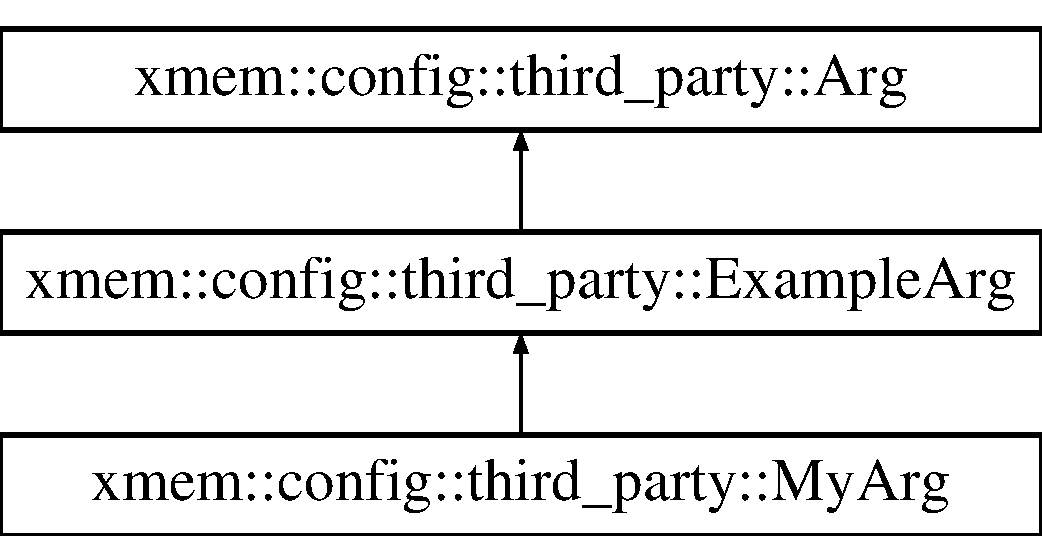
\includegraphics[height=3.000000cm]{classxmem_1_1config_1_1third__party_1_1_my_arg}
\end{center}
\end{figure}
\subsection*{Static Public Member Functions}
\begin{DoxyCompactItemize}
\item 
\hypertarget{classxmem_1_1config_1_1third__party_1_1_my_arg_aa96164ec393fdb12b359e33ee48e3c64}{static Arg\-Status \hyperlink{classxmem_1_1config_1_1third__party_1_1_my_arg_aa96164ec393fdb12b359e33ee48e3c64}{Integer} (const \hyperlink{classxmem_1_1config_1_1third__party_1_1_option}{Option} \&option, bool msg)}\label{classxmem_1_1config_1_1third__party_1_1_my_arg_aa96164ec393fdb12b359e33ee48e3c64}

\begin{DoxyCompactList}\small\item\em Checks an option that it is an integer. \end{DoxyCompactList}\item 
\hypertarget{classxmem_1_1config_1_1third__party_1_1_my_arg_a51af9350382f12100b5bd6b554c3bcf5}{static Arg\-Status \hyperlink{classxmem_1_1config_1_1third__party_1_1_my_arg_a51af9350382f12100b5bd6b554c3bcf5}{Nonnegative\-Integer} (const \hyperlink{classxmem_1_1config_1_1third__party_1_1_option}{Option} \&option, bool msg)}\label{classxmem_1_1config_1_1third__party_1_1_my_arg_a51af9350382f12100b5bd6b554c3bcf5}

\begin{DoxyCompactList}\small\item\em Checks an option that it is a nonnegative integer. \end{DoxyCompactList}\item 
\hypertarget{classxmem_1_1config_1_1third__party_1_1_my_arg_ad022660b254db34b578eb5b3fc9782a7}{static Arg\-Status \hyperlink{classxmem_1_1config_1_1third__party_1_1_my_arg_ad022660b254db34b578eb5b3fc9782a7}{Positive\-Integer} (const \hyperlink{classxmem_1_1config_1_1third__party_1_1_option}{Option} \&option, bool msg)}\label{classxmem_1_1config_1_1third__party_1_1_my_arg_ad022660b254db34b578eb5b3fc9782a7}

\begin{DoxyCompactList}\small\item\em Checks an option that it is a positive integer. \end{DoxyCompactList}\end{DoxyCompactItemize}


The documentation for this class was generated from the following file\-:\begin{DoxyCompactItemize}
\item 
src/include/\hyperlink{_my_arg_8h}{My\-Arg.\-h}\end{DoxyCompactItemize}

\hypertarget{classxmem_1_1power_1_1_native_d_r_a_m_power_reader}{}\section{xmem\+:\+:power\+:\+:Native\+D\+R\+A\+M\+Power\+Reader Class Reference}
\label{classxmem_1_1power_1_1_native_d_r_a_m_power_reader}\index{xmem\+::power\+::\+Native\+D\+R\+A\+M\+Power\+Reader@{xmem\+::power\+::\+Native\+D\+R\+A\+M\+Power\+Reader}}


A class for measuring socket-\/level D\+R\+A\+M power from the O\+S performance counter interface.  




{\ttfamily \#include $<$Native\+D\+R\+A\+M\+Power\+Reader.\+h$>$}

Inheritance diagram for xmem\+:\+:power\+:\+:Native\+D\+R\+A\+M\+Power\+Reader\+:\begin{figure}[H]
\begin{center}
\leavevmode
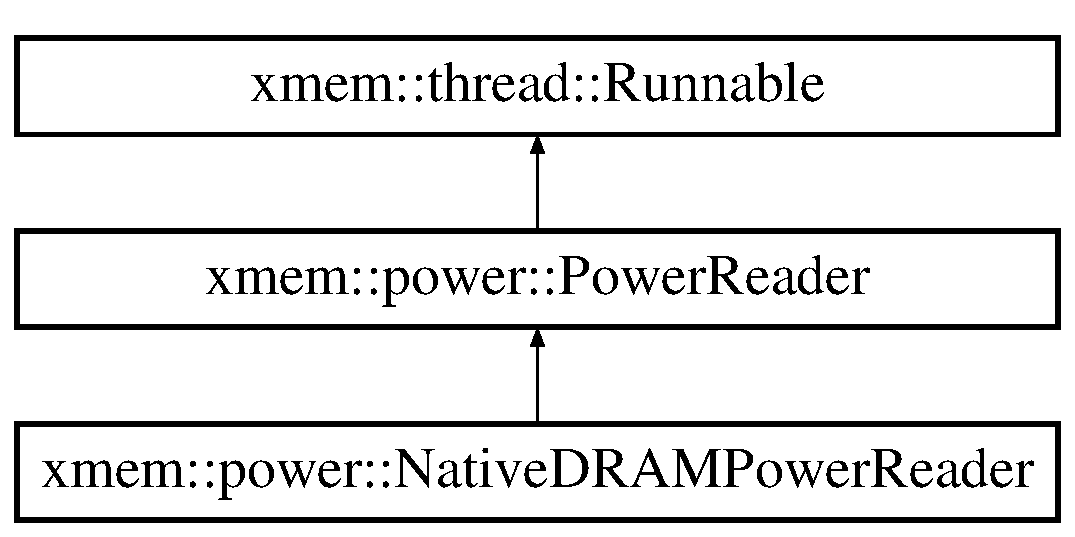
\includegraphics[height=3.000000cm]{classxmem_1_1power_1_1_native_d_r_a_m_power_reader}
\end{center}
\end{figure}
\subsection*{Public Member Functions}
\begin{DoxyCompactItemize}
\item 
\hyperlink{classxmem_1_1power_1_1_native_d_r_a_m_power_reader_a825b2e2e2a92c1c31f7e252bb5402e32}{Native\+D\+R\+A\+M\+Power\+Reader} (uint32\+\_\+t counter\+\_\+cpu\+\_\+index, double sampling\+\_\+period, double power\+\_\+units, std\+::string \hyperlink{classxmem_1_1power_1_1_power_reader_ac0f465b044512502eb1824f18d60e3e6}{name}, int32\+\_\+t cpu\+\_\+affinity)
\begin{DoxyCompactList}\small\item\em Constructor. \end{DoxyCompactList}\item 
\hypertarget{classxmem_1_1power_1_1_native_d_r_a_m_power_reader_a7b6049c41515c227cd23c815d60edb43}{}\hyperlink{classxmem_1_1power_1_1_native_d_r_a_m_power_reader_a7b6049c41515c227cd23c815d60edb43}{$\sim$\+Native\+D\+R\+A\+M\+Power\+Reader} ()\label{classxmem_1_1power_1_1_native_d_r_a_m_power_reader_a7b6049c41515c227cd23c815d60edb43}

\begin{DoxyCompactList}\small\item\em Destructor. \end{DoxyCompactList}\item 
\hypertarget{classxmem_1_1power_1_1_native_d_r_a_m_power_reader_acf3e518e39c8b90f759c674a2c81d985}{}virtual void \hyperlink{classxmem_1_1power_1_1_native_d_r_a_m_power_reader_acf3e518e39c8b90f759c674a2c81d985}{run} ()\label{classxmem_1_1power_1_1_native_d_r_a_m_power_reader_acf3e518e39c8b90f759c674a2c81d985}

\begin{DoxyCompactList}\small\item\em Starts measuring power at the rate implied by the sampling\+\_\+period passed in the constructor. Terminates when \hyperlink{classxmem_1_1power_1_1_power_reader_a5c28efc4aece34a5469d067a133920f4}{stop()} is called. \end{DoxyCompactList}\end{DoxyCompactItemize}
\subsection*{Additional Inherited Members}


\subsection{Detailed Description}
A class for measuring socket-\/level D\+R\+A\+M power from the O\+S performance counter interface. 

\subsection{Constructor \& Destructor Documentation}
\hypertarget{classxmem_1_1power_1_1_native_d_r_a_m_power_reader_a825b2e2e2a92c1c31f7e252bb5402e32}{}\index{xmem\+::power\+::\+Native\+D\+R\+A\+M\+Power\+Reader@{xmem\+::power\+::\+Native\+D\+R\+A\+M\+Power\+Reader}!Native\+D\+R\+A\+M\+Power\+Reader@{Native\+D\+R\+A\+M\+Power\+Reader}}
\index{Native\+D\+R\+A\+M\+Power\+Reader@{Native\+D\+R\+A\+M\+Power\+Reader}!xmem\+::power\+::\+Native\+D\+R\+A\+M\+Power\+Reader@{xmem\+::power\+::\+Native\+D\+R\+A\+M\+Power\+Reader}}
\subsubsection[{Native\+D\+R\+A\+M\+Power\+Reader}]{\setlength{\rightskip}{0pt plus 5cm}Native\+D\+R\+A\+M\+Power\+Reader\+::\+Native\+D\+R\+A\+M\+Power\+Reader (
\begin{DoxyParamCaption}
\item[{uint32\+\_\+t}]{counter\+\_\+cpu\+\_\+index, }
\item[{double}]{sampling\+\_\+period, }
\item[{double}]{power\+\_\+units, }
\item[{std\+::string}]{name, }
\item[{int32\+\_\+t}]{cpu\+\_\+affinity}
\end{DoxyParamCaption}
)}\label{classxmem_1_1power_1_1_native_d_r_a_m_power_reader_a825b2e2e2a92c1c31f7e252bb5402e32}


Constructor. 


\begin{DoxyParams}{Parameters}
{\em counter\+\_\+cpu\+\_\+index} & Which C\+P\+U\textquotesingle{}s D\+R\+A\+M power counter to sample. A single hardware counter might be shared across different C\+P\+Us. \\
\hline
{\em sampling\+\_\+period} & The time between power samples in seconds. \\
\hline
{\em power\+\_\+units} & The power units for each sample in watts. \\
\hline
{\em cpu\+\_\+affinity} & The C\+P\+U affinity for this object\textquotesingle{}s \hyperlink{classxmem_1_1power_1_1_native_d_r_a_m_power_reader_acf3e518e39c8b90f759c674a2c81d985}{run()} method for any thread that calls it. If negative, no affinity preference. \\
\hline
\end{DoxyParams}


The documentation for this class was generated from the following files\+:\begin{DoxyCompactItemize}
\item 
src/include/\hyperlink{_native_d_r_a_m_power_reader_8h}{Native\+D\+R\+A\+M\+Power\+Reader.\+h}\item 
src/\hyperlink{_native_d_r_a_m_power_reader_8cpp}{Native\+D\+R\+A\+M\+Power\+Reader.\+cpp}\end{DoxyCompactItemize}

\hypertarget{classxmem_1_1config_1_1third__party_1_1_option}{\section{xmem\-:\-:config\-:\-:third\-\_\-party\-:\-:Option Class Reference}
\label{classxmem_1_1config_1_1third__party_1_1_option}\index{xmem\-::config\-::third\-\_\-party\-::\-Option@{xmem\-::config\-::third\-\_\-party\-::\-Option}}
}


A parsed option from the command line together with its argument if it has one.  




{\ttfamily \#include $<$optionparser.\-h$>$}

\subsection*{Public Member Functions}
\begin{DoxyCompactItemize}
\item 
int \hyperlink{classxmem_1_1config_1_1third__party_1_1_option_a4d80ee182577f0dacfbd617cfd714833}{type} () const 
\begin{DoxyCompactList}\small\item\em Returns \hyperlink{structxmem_1_1config_1_1third__party_1_1_descriptor_a4b9e9a5c9b08ef575ea4f603c54bff63}{Descriptor\-::type} of this \hyperlink{classxmem_1_1config_1_1third__party_1_1_option}{Option}'s \hyperlink{structxmem_1_1config_1_1third__party_1_1_descriptor}{Descriptor}, or 0 if this \hyperlink{classxmem_1_1config_1_1third__party_1_1_option}{Option} is invalid (unused). \end{DoxyCompactList}\item 
\hypertarget{classxmem_1_1config_1_1third__party_1_1_option_a7debc43bf253931503da7efd4bf478e9}{int \hyperlink{classxmem_1_1config_1_1third__party_1_1_option_a7debc43bf253931503da7efd4bf478e9}{index} () const }\label{classxmem_1_1config_1_1third__party_1_1_option_a7debc43bf253931503da7efd4bf478e9}

\begin{DoxyCompactList}\small\item\em Returns \hyperlink{structxmem_1_1config_1_1third__party_1_1_descriptor_aacf3d44f35c61f22be65da078f60734b}{Descriptor\-::index} of this \hyperlink{classxmem_1_1config_1_1third__party_1_1_option}{Option}'s \hyperlink{structxmem_1_1config_1_1third__party_1_1_descriptor}{Descriptor}, or -\/1 if this \hyperlink{classxmem_1_1config_1_1third__party_1_1_option}{Option} is invalid (unused). \end{DoxyCompactList}\item 
int \hyperlink{classxmem_1_1config_1_1third__party_1_1_option_ae10dde777907e632276e585539047576}{count} ()
\begin{DoxyCompactList}\small\item\em Returns the number of times this \hyperlink{classxmem_1_1config_1_1third__party_1_1_option}{Option} (or others with the same \hyperlink{structxmem_1_1config_1_1third__party_1_1_descriptor_aacf3d44f35c61f22be65da078f60734b}{Descriptor\-::index}) occurs in the argument vector. \end{DoxyCompactList}\item 
bool \hyperlink{classxmem_1_1config_1_1third__party_1_1_option_aa15a4bdfb804f7d7431d0895ed4068d2}{is\-First} () const 
\begin{DoxyCompactList}\small\item\em Returns true iff this is the first element of the linked list. \end{DoxyCompactList}\item 
bool \hyperlink{classxmem_1_1config_1_1third__party_1_1_option_a3aa92482d52df551ceb135d9efb34a7f}{is\-Last} () const 
\begin{DoxyCompactList}\small\item\em Returns true iff this is the last element of the linked list. \end{DoxyCompactList}\item 
\hyperlink{classxmem_1_1config_1_1third__party_1_1_option}{Option} $\ast$ \hyperlink{classxmem_1_1config_1_1third__party_1_1_option_a6c8907c4faaf8c099d556db54bfca1a5}{first} ()
\begin{DoxyCompactList}\small\item\em Returns a pointer to the first element of the linked list. \end{DoxyCompactList}\item 
\hyperlink{classxmem_1_1config_1_1third__party_1_1_option}{Option} $\ast$ \hyperlink{classxmem_1_1config_1_1third__party_1_1_option_a79bd212eaf002df298da1b3b46e34cea}{last} ()
\begin{DoxyCompactList}\small\item\em Returns a pointer to the last element of the linked list. \end{DoxyCompactList}\item 
\hyperlink{classxmem_1_1config_1_1third__party_1_1_option}{Option} $\ast$ \hyperlink{classxmem_1_1config_1_1third__party_1_1_option_a51c55046e8f111be3e329f798d0f72b9}{prev} ()
\begin{DoxyCompactList}\small\item\em Returns a pointer to the previous element of the linked list or N\-U\-L\-L if called on \hyperlink{classxmem_1_1config_1_1third__party_1_1_option_a6c8907c4faaf8c099d556db54bfca1a5}{first()}. \end{DoxyCompactList}\item 
\hyperlink{classxmem_1_1config_1_1third__party_1_1_option}{Option} $\ast$ \hyperlink{classxmem_1_1config_1_1third__party_1_1_option_a66a85758180b4b833dfd6574ba1a2246}{prevwrap} ()
\begin{DoxyCompactList}\small\item\em Returns a pointer to the previous element of the linked list with wrap-\/around from \hyperlink{classxmem_1_1config_1_1third__party_1_1_option_a6c8907c4faaf8c099d556db54bfca1a5}{first()} to \hyperlink{classxmem_1_1config_1_1third__party_1_1_option_a79bd212eaf002df298da1b3b46e34cea}{last()}. \end{DoxyCompactList}\item 
\hyperlink{classxmem_1_1config_1_1third__party_1_1_option}{Option} $\ast$ \hyperlink{classxmem_1_1config_1_1third__party_1_1_option_af9c5d2de03863bbcdc05a1d6771f1f36}{next} ()
\begin{DoxyCompactList}\small\item\em Returns a pointer to the next element of the linked list or N\-U\-L\-L if called on \hyperlink{classxmem_1_1config_1_1third__party_1_1_option_a79bd212eaf002df298da1b3b46e34cea}{last()}. \end{DoxyCompactList}\item 
\hyperlink{classxmem_1_1config_1_1third__party_1_1_option}{Option} $\ast$ \hyperlink{classxmem_1_1config_1_1third__party_1_1_option_ae4da74e185cee05d6e3eeda723b39b50}{nextwrap} ()
\begin{DoxyCompactList}\small\item\em Returns a pointer to the next element of the linked list with wrap-\/around from \hyperlink{classxmem_1_1config_1_1third__party_1_1_option_a79bd212eaf002df298da1b3b46e34cea}{last()} to \hyperlink{classxmem_1_1config_1_1third__party_1_1_option_a6c8907c4faaf8c099d556db54bfca1a5}{first()}. \end{DoxyCompactList}\item 
void \hyperlink{classxmem_1_1config_1_1third__party_1_1_option_ac8fcf58435fb4e82ce937074af8198ac}{append} (\hyperlink{classxmem_1_1config_1_1third__party_1_1_option}{Option} $\ast$new\-\_\-last)
\begin{DoxyCompactList}\small\item\em Makes {\ttfamily new\-\_\-last} the new \hyperlink{classxmem_1_1config_1_1third__party_1_1_option_a79bd212eaf002df298da1b3b46e34cea}{last()} by chaining it into the list after \hyperlink{classxmem_1_1config_1_1third__party_1_1_option_a79bd212eaf002df298da1b3b46e34cea}{last()}. \end{DoxyCompactList}\item 
\hyperlink{classxmem_1_1config_1_1third__party_1_1_option_ae2be6cea552bb7b55fc4b264f5720911}{operator const Option $\ast$} () const 
\begin{DoxyCompactList}\small\item\em Casts from \hyperlink{classxmem_1_1config_1_1third__party_1_1_option}{Option} to const Option$\ast$ but only if this \hyperlink{classxmem_1_1config_1_1third__party_1_1_option}{Option} is valid. \end{DoxyCompactList}\item 
\hyperlink{classxmem_1_1config_1_1third__party_1_1_option_aca15f5c3126a45ea8e24dae817ebea7d}{operator Option $\ast$} ()
\begin{DoxyCompactList}\small\item\em Casts from \hyperlink{classxmem_1_1config_1_1third__party_1_1_option}{Option} to Option$\ast$ but only if this \hyperlink{classxmem_1_1config_1_1third__party_1_1_option}{Option} is valid. \end{DoxyCompactList}\item 
\hypertarget{classxmem_1_1config_1_1third__party_1_1_option_a49ea7c71e3f980214ad2ef4cca3c6662}{\hyperlink{classxmem_1_1config_1_1third__party_1_1_option_a49ea7c71e3f980214ad2ef4cca3c6662}{Option} ()}\label{classxmem_1_1config_1_1third__party_1_1_option_a49ea7c71e3f980214ad2ef4cca3c6662}

\begin{DoxyCompactList}\small\item\em Creates a new \hyperlink{classxmem_1_1config_1_1third__party_1_1_option}{Option} that is a one-\/element linked list and has N\-U\-L\-L \hyperlink{classxmem_1_1config_1_1third__party_1_1_option_a561317d9c847dee40c9da4a1c2065d8a}{desc}, \hyperlink{classxmem_1_1config_1_1third__party_1_1_option_aa73b73027c0a9140aeec654f3fe9aef6}{name}, \hyperlink{classxmem_1_1config_1_1third__party_1_1_option_a409f63d66d900e594dd86bcdfa9fd86a}{arg} and \hyperlink{classxmem_1_1config_1_1third__party_1_1_option_ab9c40a964cbbde704d77407446a76933}{namelen}. \end{DoxyCompactList}\item 
\hyperlink{classxmem_1_1config_1_1third__party_1_1_option_abdc9596facfb7d52699c2f34129b2633}{Option} (const \hyperlink{structxmem_1_1config_1_1third__party_1_1_descriptor}{Descriptor} $\ast$desc\-\_\-, const char $\ast$name\-\_\-, const char $\ast$arg\-\_\-)
\begin{DoxyCompactList}\small\item\em Creates a new \hyperlink{classxmem_1_1config_1_1third__party_1_1_option}{Option} that is a one-\/element linked list and has the given values for \hyperlink{classxmem_1_1config_1_1third__party_1_1_option_a561317d9c847dee40c9da4a1c2065d8a}{desc}, \hyperlink{classxmem_1_1config_1_1third__party_1_1_option_aa73b73027c0a9140aeec654f3fe9aef6}{name} and \hyperlink{classxmem_1_1config_1_1third__party_1_1_option_a409f63d66d900e594dd86bcdfa9fd86a}{arg}. \end{DoxyCompactList}\item 
void \hyperlink{classxmem_1_1config_1_1third__party_1_1_option_a2667e3b7783d722e9967e8ace40931cb}{operator=} (const \hyperlink{classxmem_1_1config_1_1third__party_1_1_option}{Option} \&orig)
\begin{DoxyCompactList}\small\item\em Makes {\ttfamily $\ast$this} a copy of {\ttfamily orig} except for the linked list pointers. \end{DoxyCompactList}\item 
\hyperlink{classxmem_1_1config_1_1third__party_1_1_option_a8e927ab73561c9fe9973ac86bb3e3fd0}{Option} (const \hyperlink{classxmem_1_1config_1_1third__party_1_1_option}{Option} \&orig)
\begin{DoxyCompactList}\small\item\em Makes {\ttfamily $\ast$this} a copy of {\ttfamily orig} except for the linked list pointers. \end{DoxyCompactList}\end{DoxyCompactItemize}
\subsection*{Public Attributes}
\begin{DoxyCompactItemize}
\item 
const \hyperlink{structxmem_1_1config_1_1third__party_1_1_descriptor}{Descriptor} $\ast$ \hyperlink{classxmem_1_1config_1_1third__party_1_1_option_a561317d9c847dee40c9da4a1c2065d8a}{desc}
\begin{DoxyCompactList}\small\item\em Pointer to this \hyperlink{classxmem_1_1config_1_1third__party_1_1_option}{Option}'s \hyperlink{structxmem_1_1config_1_1third__party_1_1_descriptor}{Descriptor}. \end{DoxyCompactList}\item 
const char $\ast$ \hyperlink{classxmem_1_1config_1_1third__party_1_1_option_aa73b73027c0a9140aeec654f3fe9aef6}{name}
\begin{DoxyCompactList}\small\item\em The name of the option as used on the command line. \end{DoxyCompactList}\item 
const char $\ast$ \hyperlink{classxmem_1_1config_1_1third__party_1_1_option_a409f63d66d900e594dd86bcdfa9fd86a}{arg}
\begin{DoxyCompactList}\small\item\em Pointer to this \hyperlink{classxmem_1_1config_1_1third__party_1_1_option}{Option}'s argument (if any). \end{DoxyCompactList}\item 
int \hyperlink{classxmem_1_1config_1_1third__party_1_1_option_ab9c40a964cbbde704d77407446a76933}{namelen}
\begin{DoxyCompactList}\small\item\em The length of the option \hyperlink{classxmem_1_1config_1_1third__party_1_1_option_aa73b73027c0a9140aeec654f3fe9aef6}{name}. \end{DoxyCompactList}\end{DoxyCompactItemize}


\subsection{Detailed Description}
A parsed option from the command line together with its argument if it has one. 

The \hyperlink{classxmem_1_1config_1_1third__party_1_1_parser}{Parser} chains all parsed options with the same \hyperlink{structxmem_1_1config_1_1third__party_1_1_descriptor_aacf3d44f35c61f22be65da078f60734b}{Descriptor\-::index} together to form a linked list. This allows you to easily implement all of the common ways of handling repeated options and enable/disable pairs.

\begin{DoxyItemize}
\item Test for presence of a switch in the argument vector\-: 
\begin{DoxyCode}
\textcolor{keywordflow}{if} ( options[QUIET] ) ... 
\end{DoxyCode}
 \item Evaluate --enable-\/foo/--disable-\/foo pair where the last one used wins\-: 
\begin{DoxyCode}
\textcolor{keywordflow}{if} ( options[FOO].\hyperlink{classxmem_1_1config_1_1third__party_1_1_option_a79bd212eaf002df298da1b3b46e34cea}{last}()->\hyperlink{classxmem_1_1config_1_1third__party_1_1_option_a4d80ee182577f0dacfbd617cfd714833}{type}() == DISABLE ) ... 
\end{DoxyCode}
 \item Cumulative option (-\/v verbose, -\/vv more verbose, -\/vvv even more verbose)\-: 
\begin{DoxyCode}
\textcolor{keywordtype}{int} verbosity = options[\hyperlink{common_8h_a42f8c497a1968074f38bf5055c650dca}{VERBOSE}].count(); 
\end{DoxyCode}
 \item Iterate over all --file=$<$fname$>$ arguments\-: 
\begin{DoxyCode}
\textcolor{keywordflow}{for} (\hyperlink{classxmem_1_1config_1_1third__party_1_1_option_a49ea7c71e3f980214ad2ef4cca3c6662}{Option}* opt = options[FILE]; opt; opt = opt->next())
 fname = opt->arg; ... 
\end{DoxyCode}
 \end{DoxyItemize}


\subsection{Constructor \& Destructor Documentation}
\hypertarget{classxmem_1_1config_1_1third__party_1_1_option_abdc9596facfb7d52699c2f34129b2633}{\index{xmem\-::config\-::third\-\_\-party\-::\-Option@{xmem\-::config\-::third\-\_\-party\-::\-Option}!Option@{Option}}
\index{Option@{Option}!xmem::config::third_party::Option@{xmem\-::config\-::third\-\_\-party\-::\-Option}}
\subsubsection[{Option}]{\setlength{\rightskip}{0pt plus 5cm}xmem\-::config\-::third\-\_\-party\-::\-Option\-::\-Option (
\begin{DoxyParamCaption}
\item[{const {\bf Descriptor} $\ast$}]{desc\-\_\-, }
\item[{const char $\ast$}]{name\-\_\-, }
\item[{const char $\ast$}]{arg\-\_\-}
\end{DoxyParamCaption}
)\hspace{0.3cm}{\ttfamily [inline]}}}\label{classxmem_1_1config_1_1third__party_1_1_option_abdc9596facfb7d52699c2f34129b2633}


Creates a new \hyperlink{classxmem_1_1config_1_1third__party_1_1_option}{Option} that is a one-\/element linked list and has the given values for \hyperlink{classxmem_1_1config_1_1third__party_1_1_option_a561317d9c847dee40c9da4a1c2065d8a}{desc}, \hyperlink{classxmem_1_1config_1_1third__party_1_1_option_aa73b73027c0a9140aeec654f3fe9aef6}{name} and \hyperlink{classxmem_1_1config_1_1third__party_1_1_option_a409f63d66d900e594dd86bcdfa9fd86a}{arg}. 

If {\ttfamily name\-\_\-} points at a character other than '-\/' it will be assumed to refer to a short option and \hyperlink{classxmem_1_1config_1_1third__party_1_1_option_ab9c40a964cbbde704d77407446a76933}{namelen} will be set to 1. Otherwise the length will extend to the first '=' character or the string's 0-\/terminator. \hypertarget{classxmem_1_1config_1_1third__party_1_1_option_a8e927ab73561c9fe9973ac86bb3e3fd0}{\index{xmem\-::config\-::third\-\_\-party\-::\-Option@{xmem\-::config\-::third\-\_\-party\-::\-Option}!Option@{Option}}
\index{Option@{Option}!xmem::config::third_party::Option@{xmem\-::config\-::third\-\_\-party\-::\-Option}}
\subsubsection[{Option}]{\setlength{\rightskip}{0pt plus 5cm}xmem\-::config\-::third\-\_\-party\-::\-Option\-::\-Option (
\begin{DoxyParamCaption}
\item[{const {\bf Option} \&}]{orig}
\end{DoxyParamCaption}
)\hspace{0.3cm}{\ttfamily [inline]}}}\label{classxmem_1_1config_1_1third__party_1_1_option_a8e927ab73561c9fe9973ac86bb3e3fd0}


Makes {\ttfamily $\ast$this} a copy of {\ttfamily orig} except for the linked list pointers. 

After this operation {\ttfamily $\ast$this} will be a one-\/element linked list. 

\subsection{Member Function Documentation}
\hypertarget{classxmem_1_1config_1_1third__party_1_1_option_ac8fcf58435fb4e82ce937074af8198ac}{\index{xmem\-::config\-::third\-\_\-party\-::\-Option@{xmem\-::config\-::third\-\_\-party\-::\-Option}!append@{append}}
\index{append@{append}!xmem::config::third_party::Option@{xmem\-::config\-::third\-\_\-party\-::\-Option}}
\subsubsection[{append}]{\setlength{\rightskip}{0pt plus 5cm}void xmem\-::config\-::third\-\_\-party\-::\-Option\-::append (
\begin{DoxyParamCaption}
\item[{{\bf Option} $\ast$}]{new\-\_\-last}
\end{DoxyParamCaption}
)\hspace{0.3cm}{\ttfamily [inline]}}}\label{classxmem_1_1config_1_1third__party_1_1_option_ac8fcf58435fb4e82ce937074af8198ac}


Makes {\ttfamily new\-\_\-last} the new \hyperlink{classxmem_1_1config_1_1third__party_1_1_option_a79bd212eaf002df298da1b3b46e34cea}{last()} by chaining it into the list after \hyperlink{classxmem_1_1config_1_1third__party_1_1_option_a79bd212eaf002df298da1b3b46e34cea}{last()}. 

It doesn't matter which element you call \hyperlink{classxmem_1_1config_1_1third__party_1_1_option_ac8fcf58435fb4e82ce937074af8198ac}{append()} on. The new element will always be appended to \hyperlink{classxmem_1_1config_1_1third__party_1_1_option_a79bd212eaf002df298da1b3b46e34cea}{last()}.

\begin{DoxyAttention}{Attention}
{\ttfamily new\-\_\-last} must not yet be part of a list, or that list will become corrupted, because this method does not unchain {\ttfamily new\-\_\-last} from an existing list. 
\end{DoxyAttention}
\hypertarget{classxmem_1_1config_1_1third__party_1_1_option_ae10dde777907e632276e585539047576}{\index{xmem\-::config\-::third\-\_\-party\-::\-Option@{xmem\-::config\-::third\-\_\-party\-::\-Option}!count@{count}}
\index{count@{count}!xmem::config::third_party::Option@{xmem\-::config\-::third\-\_\-party\-::\-Option}}
\subsubsection[{count}]{\setlength{\rightskip}{0pt plus 5cm}int xmem\-::config\-::third\-\_\-party\-::\-Option\-::count (
\begin{DoxyParamCaption}
{}
\end{DoxyParamCaption}
)\hspace{0.3cm}{\ttfamily [inline]}}}\label{classxmem_1_1config_1_1third__party_1_1_option_ae10dde777907e632276e585539047576}


Returns the number of times this \hyperlink{classxmem_1_1config_1_1third__party_1_1_option}{Option} (or others with the same \hyperlink{structxmem_1_1config_1_1third__party_1_1_descriptor_aacf3d44f35c61f22be65da078f60734b}{Descriptor\-::index}) occurs in the argument vector. 

This corresponds to the number of elements in the linked list this \hyperlink{classxmem_1_1config_1_1third__party_1_1_option}{Option} is part of. It doesn't matter on which element you call \hyperlink{classxmem_1_1config_1_1third__party_1_1_option_ae10dde777907e632276e585539047576}{count()}. The return value is always the same.

Use this to implement cumulative options, such as -\/v, -\/vv, -\/vvv for different verbosity levels.

Returns 0 when called for an unused/invalid option. \hypertarget{classxmem_1_1config_1_1third__party_1_1_option_a6c8907c4faaf8c099d556db54bfca1a5}{\index{xmem\-::config\-::third\-\_\-party\-::\-Option@{xmem\-::config\-::third\-\_\-party\-::\-Option}!first@{first}}
\index{first@{first}!xmem::config::third_party::Option@{xmem\-::config\-::third\-\_\-party\-::\-Option}}
\subsubsection[{first}]{\setlength{\rightskip}{0pt plus 5cm}{\bf Option}$\ast$ xmem\-::config\-::third\-\_\-party\-::\-Option\-::first (
\begin{DoxyParamCaption}
{}
\end{DoxyParamCaption}
)\hspace{0.3cm}{\ttfamily [inline]}}}\label{classxmem_1_1config_1_1third__party_1_1_option_a6c8907c4faaf8c099d556db54bfca1a5}


Returns a pointer to the first element of the linked list. 

Use this when you want the first occurrence of an option on the command line to take precedence. Note that this is not the way most programs handle options. You should probably be using \hyperlink{classxmem_1_1config_1_1third__party_1_1_option_a79bd212eaf002df298da1b3b46e34cea}{last()} instead.

\begin{DoxyNote}{Note}
This method may be called on an unused/invalid option and will return a pointer to the option itself. 
\end{DoxyNote}
\hypertarget{classxmem_1_1config_1_1third__party_1_1_option_aa15a4bdfb804f7d7431d0895ed4068d2}{\index{xmem\-::config\-::third\-\_\-party\-::\-Option@{xmem\-::config\-::third\-\_\-party\-::\-Option}!is\-First@{is\-First}}
\index{is\-First@{is\-First}!xmem::config::third_party::Option@{xmem\-::config\-::third\-\_\-party\-::\-Option}}
\subsubsection[{is\-First}]{\setlength{\rightskip}{0pt plus 5cm}bool xmem\-::config\-::third\-\_\-party\-::\-Option\-::is\-First (
\begin{DoxyParamCaption}
{}
\end{DoxyParamCaption}
) const\hspace{0.3cm}{\ttfamily [inline]}}}\label{classxmem_1_1config_1_1third__party_1_1_option_aa15a4bdfb804f7d7431d0895ed4068d2}


Returns true iff this is the first element of the linked list. 

The first element in the linked list is the first option on the command line that has the respective \hyperlink{structxmem_1_1config_1_1third__party_1_1_descriptor_aacf3d44f35c61f22be65da078f60734b}{Descriptor\-::index} value.

Returns true for an unused/invalid option. \hypertarget{classxmem_1_1config_1_1third__party_1_1_option_a3aa92482d52df551ceb135d9efb34a7f}{\index{xmem\-::config\-::third\-\_\-party\-::\-Option@{xmem\-::config\-::third\-\_\-party\-::\-Option}!is\-Last@{is\-Last}}
\index{is\-Last@{is\-Last}!xmem::config::third_party::Option@{xmem\-::config\-::third\-\_\-party\-::\-Option}}
\subsubsection[{is\-Last}]{\setlength{\rightskip}{0pt plus 5cm}bool xmem\-::config\-::third\-\_\-party\-::\-Option\-::is\-Last (
\begin{DoxyParamCaption}
{}
\end{DoxyParamCaption}
) const\hspace{0.3cm}{\ttfamily [inline]}}}\label{classxmem_1_1config_1_1third__party_1_1_option_a3aa92482d52df551ceb135d9efb34a7f}


Returns true iff this is the last element of the linked list. 

The last element in the linked list is the last option on the command line that has the respective \hyperlink{structxmem_1_1config_1_1third__party_1_1_descriptor_aacf3d44f35c61f22be65da078f60734b}{Descriptor\-::index} value.

Returns true for an unused/invalid option. \hypertarget{classxmem_1_1config_1_1third__party_1_1_option_a79bd212eaf002df298da1b3b46e34cea}{\index{xmem\-::config\-::third\-\_\-party\-::\-Option@{xmem\-::config\-::third\-\_\-party\-::\-Option}!last@{last}}
\index{last@{last}!xmem::config::third_party::Option@{xmem\-::config\-::third\-\_\-party\-::\-Option}}
\subsubsection[{last}]{\setlength{\rightskip}{0pt plus 5cm}{\bf Option}$\ast$ xmem\-::config\-::third\-\_\-party\-::\-Option\-::last (
\begin{DoxyParamCaption}
{}
\end{DoxyParamCaption}
)\hspace{0.3cm}{\ttfamily [inline]}}}\label{classxmem_1_1config_1_1third__party_1_1_option_a79bd212eaf002df298da1b3b46e34cea}


Returns a pointer to the last element of the linked list. 

Use this when you want the last occurrence of an option on the command line to take precedence. This is the most common way of handling conflicting options.

\begin{DoxyNote}{Note}
This method may be called on an unused/invalid option and will return a pointer to the option itself.
\end{DoxyNote}
\begin{DoxyParagraph}{Tip\-:}
If you have options with opposite meanings (e.\-g. {\ttfamily --enable-\/foo} and {\ttfamily --disable-\/foo}), you can assign them the same \hyperlink{structxmem_1_1config_1_1third__party_1_1_descriptor_aacf3d44f35c61f22be65da078f60734b}{Descriptor\-::index} to get them into the same list. Distinguish them by \hyperlink{structxmem_1_1config_1_1third__party_1_1_descriptor_a4b9e9a5c9b08ef575ea4f603c54bff63}{Descriptor\-::type} and all you have to do is check {\ttfamily  \hyperlink{classxmem_1_1config_1_1third__party_1_1_option_a79bd212eaf002df298da1b3b46e34cea}{last()}-\/$>$\hyperlink{classxmem_1_1config_1_1third__party_1_1_option_a4d80ee182577f0dacfbd617cfd714833}{type()} } to get the state listed last on the command line. 
\end{DoxyParagraph}
\hypertarget{classxmem_1_1config_1_1third__party_1_1_option_af9c5d2de03863bbcdc05a1d6771f1f36}{\index{xmem\-::config\-::third\-\_\-party\-::\-Option@{xmem\-::config\-::third\-\_\-party\-::\-Option}!next@{next}}
\index{next@{next}!xmem::config::third_party::Option@{xmem\-::config\-::third\-\_\-party\-::\-Option}}
\subsubsection[{next}]{\setlength{\rightskip}{0pt plus 5cm}{\bf Option}$\ast$ xmem\-::config\-::third\-\_\-party\-::\-Option\-::next (
\begin{DoxyParamCaption}
{}
\end{DoxyParamCaption}
)\hspace{0.3cm}{\ttfamily [inline]}}}\label{classxmem_1_1config_1_1third__party_1_1_option_af9c5d2de03863bbcdc05a1d6771f1f36}


Returns a pointer to the next element of the linked list or N\-U\-L\-L if called on \hyperlink{classxmem_1_1config_1_1third__party_1_1_option_a79bd212eaf002df298da1b3b46e34cea}{last()}. 

If called on \hyperlink{classxmem_1_1config_1_1third__party_1_1_option_a79bd212eaf002df298da1b3b46e34cea}{last()} this method returns N\-U\-L\-L. Otherwise it will return the option with the same \hyperlink{structxmem_1_1config_1_1third__party_1_1_descriptor_aacf3d44f35c61f22be65da078f60734b}{Descriptor\-::index} that follows this option on the command line. \hypertarget{classxmem_1_1config_1_1third__party_1_1_option_ae4da74e185cee05d6e3eeda723b39b50}{\index{xmem\-::config\-::third\-\_\-party\-::\-Option@{xmem\-::config\-::third\-\_\-party\-::\-Option}!nextwrap@{nextwrap}}
\index{nextwrap@{nextwrap}!xmem::config::third_party::Option@{xmem\-::config\-::third\-\_\-party\-::\-Option}}
\subsubsection[{nextwrap}]{\setlength{\rightskip}{0pt plus 5cm}{\bf Option}$\ast$ xmem\-::config\-::third\-\_\-party\-::\-Option\-::nextwrap (
\begin{DoxyParamCaption}
{}
\end{DoxyParamCaption}
)\hspace{0.3cm}{\ttfamily [inline]}}}\label{classxmem_1_1config_1_1third__party_1_1_option_ae4da74e185cee05d6e3eeda723b39b50}


Returns a pointer to the next element of the linked list with wrap-\/around from \hyperlink{classxmem_1_1config_1_1third__party_1_1_option_a79bd212eaf002df298da1b3b46e34cea}{last()} to \hyperlink{classxmem_1_1config_1_1third__party_1_1_option_a6c8907c4faaf8c099d556db54bfca1a5}{first()}. 

If called on \hyperlink{classxmem_1_1config_1_1third__party_1_1_option_a79bd212eaf002df298da1b3b46e34cea}{last()} this method returns \hyperlink{classxmem_1_1config_1_1third__party_1_1_option_a6c8907c4faaf8c099d556db54bfca1a5}{first()}. Otherwise it will return the option with the same \hyperlink{structxmem_1_1config_1_1third__party_1_1_descriptor_aacf3d44f35c61f22be65da078f60734b}{Descriptor\-::index} that follows this option on the command line. \hypertarget{classxmem_1_1config_1_1third__party_1_1_option_ae2be6cea552bb7b55fc4b264f5720911}{\index{xmem\-::config\-::third\-\_\-party\-::\-Option@{xmem\-::config\-::third\-\_\-party\-::\-Option}!operator const Option $\ast$@{operator const Option $\ast$}}
\index{operator const Option $\ast$@{operator const Option $\ast$}!xmem::config::third_party::Option@{xmem\-::config\-::third\-\_\-party\-::\-Option}}
\subsubsection[{operator const Option $\ast$}]{\setlength{\rightskip}{0pt plus 5cm}xmem\-::config\-::third\-\_\-party\-::\-Option\-::operator const {\bf Option} $\ast$ (
\begin{DoxyParamCaption}
{}
\end{DoxyParamCaption}
) const\hspace{0.3cm}{\ttfamily [inline]}}}\label{classxmem_1_1config_1_1third__party_1_1_option_ae2be6cea552bb7b55fc4b264f5720911}


Casts from \hyperlink{classxmem_1_1config_1_1third__party_1_1_option}{Option} to const Option$\ast$ but only if this \hyperlink{classxmem_1_1config_1_1third__party_1_1_option}{Option} is valid. 

If this \hyperlink{classxmem_1_1config_1_1third__party_1_1_option}{Option} is valid (i.\-e. {\ttfamily desc!=N\-U\-L\-L}), returns this. Otherwise returns N\-U\-L\-L. This allows testing an \hyperlink{classxmem_1_1config_1_1third__party_1_1_option}{Option} directly in an if-\/clause to see if it is used\-: 
\begin{DoxyCode}
\textcolor{keywordflow}{if} (options[CREATE])
\{
  ...
\}
\end{DoxyCode}
 It also allows you to write loops like this\-: 
\begin{DoxyCode}
\textcolor{keywordflow}{for} (\hyperlink{classxmem_1_1config_1_1third__party_1_1_option_a49ea7c71e3f980214ad2ef4cca3c6662}{Option}* opt = options[FILE]; opt; opt = opt->next())
 fname = opt->arg; ... 
\end{DoxyCode}
 \hypertarget{classxmem_1_1config_1_1third__party_1_1_option_aca15f5c3126a45ea8e24dae817ebea7d}{\index{xmem\-::config\-::third\-\_\-party\-::\-Option@{xmem\-::config\-::third\-\_\-party\-::\-Option}!operator Option $\ast$@{operator Option $\ast$}}
\index{operator Option $\ast$@{operator Option $\ast$}!xmem::config::third_party::Option@{xmem\-::config\-::third\-\_\-party\-::\-Option}}
\subsubsection[{operator Option $\ast$}]{\setlength{\rightskip}{0pt plus 5cm}xmem\-::config\-::third\-\_\-party\-::\-Option\-::operator {\bf Option} $\ast$ (
\begin{DoxyParamCaption}
{}
\end{DoxyParamCaption}
)\hspace{0.3cm}{\ttfamily [inline]}}}\label{classxmem_1_1config_1_1third__party_1_1_option_aca15f5c3126a45ea8e24dae817ebea7d}


Casts from \hyperlink{classxmem_1_1config_1_1third__party_1_1_option}{Option} to Option$\ast$ but only if this \hyperlink{classxmem_1_1config_1_1third__party_1_1_option}{Option} is valid. 

If this \hyperlink{classxmem_1_1config_1_1third__party_1_1_option}{Option} is valid (i.\-e. {\ttfamily desc!=N\-U\-L\-L}), returns this. Otherwise returns N\-U\-L\-L. This allows testing an \hyperlink{classxmem_1_1config_1_1third__party_1_1_option}{Option} directly in an if-\/clause to see if it is used\-: 
\begin{DoxyCode}
\textcolor{keywordflow}{if} (options[CREATE])
\{
  ...
\}
\end{DoxyCode}
 It also allows you to write loops like this\-: 
\begin{DoxyCode}
\textcolor{keywordflow}{for} (\hyperlink{classxmem_1_1config_1_1third__party_1_1_option_a49ea7c71e3f980214ad2ef4cca3c6662}{Option}* opt = options[FILE]; opt; opt = opt->next())
 fname = opt->arg; ... 
\end{DoxyCode}
 \hypertarget{classxmem_1_1config_1_1third__party_1_1_option_a2667e3b7783d722e9967e8ace40931cb}{\index{xmem\-::config\-::third\-\_\-party\-::\-Option@{xmem\-::config\-::third\-\_\-party\-::\-Option}!operator=@{operator=}}
\index{operator=@{operator=}!xmem::config::third_party::Option@{xmem\-::config\-::third\-\_\-party\-::\-Option}}
\subsubsection[{operator=}]{\setlength{\rightskip}{0pt plus 5cm}void xmem\-::config\-::third\-\_\-party\-::\-Option\-::operator= (
\begin{DoxyParamCaption}
\item[{const {\bf Option} \&}]{orig}
\end{DoxyParamCaption}
)\hspace{0.3cm}{\ttfamily [inline]}}}\label{classxmem_1_1config_1_1third__party_1_1_option_a2667e3b7783d722e9967e8ace40931cb}


Makes {\ttfamily $\ast$this} a copy of {\ttfamily orig} except for the linked list pointers. 

After this operation {\ttfamily $\ast$this} will be a one-\/element linked list. \hypertarget{classxmem_1_1config_1_1third__party_1_1_option_a51c55046e8f111be3e329f798d0f72b9}{\index{xmem\-::config\-::third\-\_\-party\-::\-Option@{xmem\-::config\-::third\-\_\-party\-::\-Option}!prev@{prev}}
\index{prev@{prev}!xmem::config::third_party::Option@{xmem\-::config\-::third\-\_\-party\-::\-Option}}
\subsubsection[{prev}]{\setlength{\rightskip}{0pt plus 5cm}{\bf Option}$\ast$ xmem\-::config\-::third\-\_\-party\-::\-Option\-::prev (
\begin{DoxyParamCaption}
{}
\end{DoxyParamCaption}
)\hspace{0.3cm}{\ttfamily [inline]}}}\label{classxmem_1_1config_1_1third__party_1_1_option_a51c55046e8f111be3e329f798d0f72b9}


Returns a pointer to the previous element of the linked list or N\-U\-L\-L if called on \hyperlink{classxmem_1_1config_1_1third__party_1_1_option_a6c8907c4faaf8c099d556db54bfca1a5}{first()}. 

If called on \hyperlink{classxmem_1_1config_1_1third__party_1_1_option_a6c8907c4faaf8c099d556db54bfca1a5}{first()} this method returns N\-U\-L\-L. Otherwise it will return the option with the same \hyperlink{structxmem_1_1config_1_1third__party_1_1_descriptor_aacf3d44f35c61f22be65da078f60734b}{Descriptor\-::index} that precedes this option on the command line. \hypertarget{classxmem_1_1config_1_1third__party_1_1_option_a66a85758180b4b833dfd6574ba1a2246}{\index{xmem\-::config\-::third\-\_\-party\-::\-Option@{xmem\-::config\-::third\-\_\-party\-::\-Option}!prevwrap@{prevwrap}}
\index{prevwrap@{prevwrap}!xmem::config::third_party::Option@{xmem\-::config\-::third\-\_\-party\-::\-Option}}
\subsubsection[{prevwrap}]{\setlength{\rightskip}{0pt plus 5cm}{\bf Option}$\ast$ xmem\-::config\-::third\-\_\-party\-::\-Option\-::prevwrap (
\begin{DoxyParamCaption}
{}
\end{DoxyParamCaption}
)\hspace{0.3cm}{\ttfamily [inline]}}}\label{classxmem_1_1config_1_1third__party_1_1_option_a66a85758180b4b833dfd6574ba1a2246}


Returns a pointer to the previous element of the linked list with wrap-\/around from \hyperlink{classxmem_1_1config_1_1third__party_1_1_option_a6c8907c4faaf8c099d556db54bfca1a5}{first()} to \hyperlink{classxmem_1_1config_1_1third__party_1_1_option_a79bd212eaf002df298da1b3b46e34cea}{last()}. 

If called on \hyperlink{classxmem_1_1config_1_1third__party_1_1_option_a6c8907c4faaf8c099d556db54bfca1a5}{first()} this method returns \hyperlink{classxmem_1_1config_1_1third__party_1_1_option_a79bd212eaf002df298da1b3b46e34cea}{last()}. Otherwise it will return the option with the same \hyperlink{structxmem_1_1config_1_1third__party_1_1_descriptor_aacf3d44f35c61f22be65da078f60734b}{Descriptor\-::index} that precedes this option on the command line. \hypertarget{classxmem_1_1config_1_1third__party_1_1_option_a4d80ee182577f0dacfbd617cfd714833}{\index{xmem\-::config\-::third\-\_\-party\-::\-Option@{xmem\-::config\-::third\-\_\-party\-::\-Option}!type@{type}}
\index{type@{type}!xmem::config::third_party::Option@{xmem\-::config\-::third\-\_\-party\-::\-Option}}
\subsubsection[{type}]{\setlength{\rightskip}{0pt plus 5cm}int xmem\-::config\-::third\-\_\-party\-::\-Option\-::type (
\begin{DoxyParamCaption}
{}
\end{DoxyParamCaption}
) const\hspace{0.3cm}{\ttfamily [inline]}}}\label{classxmem_1_1config_1_1third__party_1_1_option_a4d80ee182577f0dacfbd617cfd714833}


Returns \hyperlink{structxmem_1_1config_1_1third__party_1_1_descriptor_a4b9e9a5c9b08ef575ea4f603c54bff63}{Descriptor\-::type} of this \hyperlink{classxmem_1_1config_1_1third__party_1_1_option}{Option}'s \hyperlink{structxmem_1_1config_1_1third__party_1_1_descriptor}{Descriptor}, or 0 if this \hyperlink{classxmem_1_1config_1_1third__party_1_1_option}{Option} is invalid (unused). 

Because this method (and \hyperlink{classxmem_1_1config_1_1third__party_1_1_option_a79bd212eaf002df298da1b3b46e34cea}{last()}, too) can be used even on unused Options with desc==0, you can (provided you arrange your types properly) switch on \hyperlink{classxmem_1_1config_1_1third__party_1_1_option_a4d80ee182577f0dacfbd617cfd714833}{type()} without testing validity first. 
\begin{DoxyCode}
\textcolor{keyword}{enum} OptionType \{ UNUSED=0, DISABLED=0, ENABLED=1 \};
\textcolor{keyword}{enum} OptionIndex \{ FOO \};
\textcolor{keyword}{const} Descriptor usage[] = \{
  \{ FOO, ENABLED,  \textcolor{stringliteral}{""}, \textcolor{stringliteral}{"enable-foo"},  \hyperlink{structxmem_1_1config_1_1third__party_1_1_arg_afdfd4a0adea72c759ec04bf5feaf3ec0}{Arg::None}, 0 \},
  \{ FOO, DISABLED, \textcolor{stringliteral}{""}, \textcolor{stringliteral}{"disable-foo"}, \hyperlink{structxmem_1_1config_1_1third__party_1_1_arg_afdfd4a0adea72c759ec04bf5feaf3ec0}{Arg::None}, 0 \},
  \{ 0, 0, 0, 0, 0, 0 \} \};
...
switch(options[FOO].\hyperlink{classxmem_1_1config_1_1third__party_1_1_option_a79bd212eaf002df298da1b3b46e34cea}{last}()->\hyperlink{classxmem_1_1config_1_1third__party_1_1_option_a4d80ee182577f0dacfbd617cfd714833}{type}()) \textcolor{comment}{// no validity check required!}
\{
  \textcolor{keywordflow}{case} ENABLED: ...
  \textcolor{keywordflow}{case} DISABLED: ...  \textcolor{comment}{// UNUSED==DISABLED !}
\}
\end{DoxyCode}
 

\subsection{Member Data Documentation}
\hypertarget{classxmem_1_1config_1_1third__party_1_1_option_a409f63d66d900e594dd86bcdfa9fd86a}{\index{xmem\-::config\-::third\-\_\-party\-::\-Option@{xmem\-::config\-::third\-\_\-party\-::\-Option}!arg@{arg}}
\index{arg@{arg}!xmem::config::third_party::Option@{xmem\-::config\-::third\-\_\-party\-::\-Option}}
\subsubsection[{arg}]{\setlength{\rightskip}{0pt plus 5cm}const char$\ast$ xmem\-::config\-::third\-\_\-party\-::\-Option\-::arg}}\label{classxmem_1_1config_1_1third__party_1_1_option_a409f63d66d900e594dd86bcdfa9fd86a}


Pointer to this \hyperlink{classxmem_1_1config_1_1third__party_1_1_option}{Option}'s argument (if any). 

N\-U\-L\-L if this option has no argument. Do not confuse this with the empty string which is a valid argument. \hypertarget{classxmem_1_1config_1_1third__party_1_1_option_a561317d9c847dee40c9da4a1c2065d8a}{\index{xmem\-::config\-::third\-\_\-party\-::\-Option@{xmem\-::config\-::third\-\_\-party\-::\-Option}!desc@{desc}}
\index{desc@{desc}!xmem::config::third_party::Option@{xmem\-::config\-::third\-\_\-party\-::\-Option}}
\subsubsection[{desc}]{\setlength{\rightskip}{0pt plus 5cm}const {\bf Descriptor}$\ast$ xmem\-::config\-::third\-\_\-party\-::\-Option\-::desc}}\label{classxmem_1_1config_1_1third__party_1_1_option_a561317d9c847dee40c9da4a1c2065d8a}


Pointer to this \hyperlink{classxmem_1_1config_1_1third__party_1_1_option}{Option}'s \hyperlink{structxmem_1_1config_1_1third__party_1_1_descriptor}{Descriptor}. 

Remember that the first dummy descriptor (see \hyperlink{structxmem_1_1config_1_1third__party_1_1_descriptor_a7246a4bfc669f68bb406dece398be7bb}{Descriptor\-::longopt}) is used for unknown options.

\begin{DoxyAttention}{Attention}
{\ttfamily desc==N\-U\-L\-L} signals that this \hyperlink{classxmem_1_1config_1_1third__party_1_1_option}{Option} is unused. This is the default state of elements in the result array. You don't need to test {\ttfamily desc} explicitly. You can simply write something like this\-: 
\begin{DoxyCode}
\textcolor{keywordflow}{if} (options[CREATE])
\{
  ...
\}
\end{DoxyCode}
 This works because of {\ttfamily  operator const Option$\ast$() }. 
\end{DoxyAttention}
\hypertarget{classxmem_1_1config_1_1third__party_1_1_option_aa73b73027c0a9140aeec654f3fe9aef6}{\index{xmem\-::config\-::third\-\_\-party\-::\-Option@{xmem\-::config\-::third\-\_\-party\-::\-Option}!name@{name}}
\index{name@{name}!xmem::config::third_party::Option@{xmem\-::config\-::third\-\_\-party\-::\-Option}}
\subsubsection[{name}]{\setlength{\rightskip}{0pt plus 5cm}const char$\ast$ xmem\-::config\-::third\-\_\-party\-::\-Option\-::name}}\label{classxmem_1_1config_1_1third__party_1_1_option_aa73b73027c0a9140aeec654f3fe9aef6}


The name of the option as used on the command line. 

The main purpose of this string is to be presented to the user in messages.

In the case of a long option, this is the actual {\ttfamily argv} pointer, i.\-e. the first character is a '-\/'. In the case of a short option this points to the option character within the {\ttfamily argv} string.

Note that in the case of a short option group or an attached option argument, this string will contain additional characters following the actual name. Use \hyperlink{classxmem_1_1config_1_1third__party_1_1_option_ab9c40a964cbbde704d77407446a76933}{namelen} to filter out the actual option name only. \hypertarget{classxmem_1_1config_1_1third__party_1_1_option_ab9c40a964cbbde704d77407446a76933}{\index{xmem\-::config\-::third\-\_\-party\-::\-Option@{xmem\-::config\-::third\-\_\-party\-::\-Option}!namelen@{namelen}}
\index{namelen@{namelen}!xmem::config::third_party::Option@{xmem\-::config\-::third\-\_\-party\-::\-Option}}
\subsubsection[{namelen}]{\setlength{\rightskip}{0pt plus 5cm}int xmem\-::config\-::third\-\_\-party\-::\-Option\-::namelen}}\label{classxmem_1_1config_1_1third__party_1_1_option_ab9c40a964cbbde704d77407446a76933}


The length of the option \hyperlink{classxmem_1_1config_1_1third__party_1_1_option_aa73b73027c0a9140aeec654f3fe9aef6}{name}. 

Because \hyperlink{classxmem_1_1config_1_1third__party_1_1_option_aa73b73027c0a9140aeec654f3fe9aef6}{name} points into the actual {\ttfamily argv} string, the option name may be followed by more characters (e.\-g. other short options in the same short option group). This value is the number of bytes (not characters!) that are part of the actual name.

For a short option, this length is always 1. For a long option this length is always at least 2 if single minus long options are permitted and at least 3 if they are disabled.

\begin{DoxyNote}{Note}
In the pathological case of a minus within a short option group (e.\-g. {\ttfamily -\/xf-\/z}), this length is incorrect, because this case will be misinterpreted as a long option and the name will therefore extend to the string's 0-\/terminator or a following '=" character if there is one. This is irrelevant for most uses of \hyperlink{classxmem_1_1config_1_1third__party_1_1_option_aa73b73027c0a9140aeec654f3fe9aef6}{name} and {\ttfamily namelen}. If you really need to distinguish the case of a long and a short option, compare \hyperlink{classxmem_1_1config_1_1third__party_1_1_option_aa73b73027c0a9140aeec654f3fe9aef6}{name} to the {\ttfamily argv} pointers. A long option's {\ttfamily name} is always identical to one of them, whereas a short option's is never. 
\end{DoxyNote}


The documentation for this class was generated from the following file\-:\begin{DoxyCompactItemize}
\item 
src/include/\hyperlink{optionparser_8h}{optionparser.\-h}\end{DoxyCompactItemize}

\hypertarget{structxmem_1_1config_1_1third__party_1_1_print_usage_implementation_1_1_o_stream_writer}{}\section{xmem\+:\+:config\+:\+:third\+\_\+party\+:\+:Print\+Usage\+Implementation\+:\+:O\+Stream\+Writer$<$ O\+Stream $>$ Struct Template Reference}
\label{structxmem_1_1config_1_1third__party_1_1_print_usage_implementation_1_1_o_stream_writer}\index{xmem\+::config\+::third\+\_\+party\+::\+Print\+Usage\+Implementation\+::\+O\+Stream\+Writer$<$ O\+Stream $>$@{xmem\+::config\+::third\+\_\+party\+::\+Print\+Usage\+Implementation\+::\+O\+Stream\+Writer$<$ O\+Stream $>$}}
Inheritance diagram for xmem\+:\+:config\+:\+:third\+\_\+party\+:\+:Print\+Usage\+Implementation\+:\+:O\+Stream\+Writer$<$ O\+Stream $>$\+:\begin{figure}[H]
\begin{center}
\leavevmode
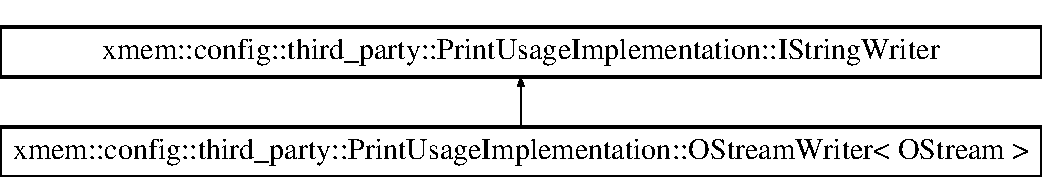
\includegraphics[height=2.000000cm]{structxmem_1_1config_1_1third__party_1_1_print_usage_implementation_1_1_o_stream_writer}
\end{center}
\end{figure}
\subsection*{Public Member Functions}
\begin{DoxyCompactItemize}
\item 
\hypertarget{structxmem_1_1config_1_1third__party_1_1_print_usage_implementation_1_1_o_stream_writer_a3b530bd8c2066ce1e77ccdd48f593f8d}{}virtual void \hyperlink{structxmem_1_1config_1_1third__party_1_1_print_usage_implementation_1_1_o_stream_writer_a3b530bd8c2066ce1e77ccdd48f593f8d}{operator()} (const char $\ast$str, int size)\label{structxmem_1_1config_1_1third__party_1_1_print_usage_implementation_1_1_o_stream_writer_a3b530bd8c2066ce1e77ccdd48f593f8d}

\begin{DoxyCompactList}\small\item\em Writes the given number of chars beginning at the given pointer somewhere. \end{DoxyCompactList}\item 
\hypertarget{structxmem_1_1config_1_1third__party_1_1_print_usage_implementation_1_1_o_stream_writer_a44255b54f77d5ec3fecc583615bc222d}{}{\bfseries O\+Stream\+Writer} (O\+Stream \&o)\label{structxmem_1_1config_1_1third__party_1_1_print_usage_implementation_1_1_o_stream_writer_a44255b54f77d5ec3fecc583615bc222d}

\end{DoxyCompactItemize}
\subsection*{Public Attributes}
\begin{DoxyCompactItemize}
\item 
\hypertarget{structxmem_1_1config_1_1third__party_1_1_print_usage_implementation_1_1_o_stream_writer_ab85a98667ea62652a59042c8ee354ab5}{}O\+Stream \& {\bfseries ostream}\label{structxmem_1_1config_1_1third__party_1_1_print_usage_implementation_1_1_o_stream_writer_ab85a98667ea62652a59042c8ee354ab5}

\end{DoxyCompactItemize}


The documentation for this struct was generated from the following file\+:\begin{DoxyCompactItemize}
\item 
src/config/third\+\_\+party/\hyperlink{optionparser_8h}{optionparser.\+h}\end{DoxyCompactItemize}

\hypertarget{classxmem_1_1config_1_1third__party_1_1_parser}{}\section{xmem\+:\+:config\+:\+:third\+\_\+party\+:\+:Parser Class Reference}
\label{classxmem_1_1config_1_1third__party_1_1_parser}\index{xmem\+::config\+::third\+\_\+party\+::\+Parser@{xmem\+::config\+::third\+\_\+party\+::\+Parser}}


Checks argument vectors for validity and parses them into data structures that are easier to work with.  




{\ttfamily \#include $<$optionparser.\+h$>$}

\subsection*{Classes}
\begin{DoxyCompactItemize}
\item 
struct \hyperlink{structxmem_1_1config_1_1third__party_1_1_parser_1_1_action}{Action}
\item 
class \hyperlink{classxmem_1_1config_1_1third__party_1_1_parser_1_1_store_option_action}{Store\+Option\+Action}
\end{DoxyCompactItemize}
\subsection*{Public Member Functions}
\begin{DoxyCompactItemize}
\item 
\hypertarget{classxmem_1_1config_1_1third__party_1_1_parser_ad88ba9ed583f79c279e84e823ab3864f}{}\hyperlink{classxmem_1_1config_1_1third__party_1_1_parser_ad88ba9ed583f79c279e84e823ab3864f}{Parser} ()\label{classxmem_1_1config_1_1third__party_1_1_parser_ad88ba9ed583f79c279e84e823ab3864f}

\begin{DoxyCompactList}\small\item\em Creates a new \hyperlink{classxmem_1_1config_1_1third__party_1_1_parser}{Parser}. \end{DoxyCompactList}\item 
\hyperlink{classxmem_1_1config_1_1third__party_1_1_parser_ab6131802b5bacfb921963abd183b5c85}{Parser} (bool gnu, const \hyperlink{structxmem_1_1config_1_1third__party_1_1_descriptor}{Descriptor} usage\mbox{[}$\,$\mbox{]}, int argc, const char $\ast$$\ast$argv, \hyperlink{classxmem_1_1config_1_1third__party_1_1_option}{Option} options\mbox{[}$\,$\mbox{]}, \hyperlink{classxmem_1_1config_1_1third__party_1_1_option}{Option} buffer\mbox{[}$\,$\mbox{]}, int min\+\_\+abbr\+\_\+len=0, bool single\+\_\+minus\+\_\+longopt=false, int bufmax=-\/1)
\begin{DoxyCompactList}\small\item\em Creates a new \hyperlink{classxmem_1_1config_1_1third__party_1_1_parser}{Parser} and immediately parses the given argument vector. \end{DoxyCompactList}\item 
\hypertarget{classxmem_1_1config_1_1third__party_1_1_parser_ae9669add72032bffff977e904b69f70a}{}\hyperlink{classxmem_1_1config_1_1third__party_1_1_parser_ae9669add72032bffff977e904b69f70a}{Parser} (bool gnu, const \hyperlink{structxmem_1_1config_1_1third__party_1_1_descriptor}{Descriptor} usage\mbox{[}$\,$\mbox{]}, int argc, char $\ast$$\ast$argv, \hyperlink{classxmem_1_1config_1_1third__party_1_1_option}{Option} options\mbox{[}$\,$\mbox{]}, \hyperlink{classxmem_1_1config_1_1third__party_1_1_option}{Option} buffer\mbox{[}$\,$\mbox{]}, int min\+\_\+abbr\+\_\+len=0, bool single\+\_\+minus\+\_\+longopt=false, int bufmax=-\/1)\label{classxmem_1_1config_1_1third__party_1_1_parser_ae9669add72032bffff977e904b69f70a}

\begin{DoxyCompactList}\small\item\em \hyperlink{classxmem_1_1config_1_1third__party_1_1_parser}{Parser}(...) with non-\/const argv. \end{DoxyCompactList}\item 
\hypertarget{classxmem_1_1config_1_1third__party_1_1_parser_a3d0990e00bad445fb5753ace6283d497}{}\hyperlink{classxmem_1_1config_1_1third__party_1_1_parser_a3d0990e00bad445fb5753ace6283d497}{Parser} (const \hyperlink{structxmem_1_1config_1_1third__party_1_1_descriptor}{Descriptor} usage\mbox{[}$\,$\mbox{]}, int argc, const char $\ast$$\ast$argv, \hyperlink{classxmem_1_1config_1_1third__party_1_1_option}{Option} options\mbox{[}$\,$\mbox{]}, \hyperlink{classxmem_1_1config_1_1third__party_1_1_option}{Option} buffer\mbox{[}$\,$\mbox{]}, int min\+\_\+abbr\+\_\+len=0, bool single\+\_\+minus\+\_\+longopt=false, int bufmax=-\/1)\label{classxmem_1_1config_1_1third__party_1_1_parser_a3d0990e00bad445fb5753ace6283d497}

\begin{DoxyCompactList}\small\item\em P\+O\+S\+I\+X \hyperlink{classxmem_1_1config_1_1third__party_1_1_parser}{Parser}(...) (gnu==false). \end{DoxyCompactList}\item 
\hypertarget{classxmem_1_1config_1_1third__party_1_1_parser_ad3d40c69fbb64462daf43b84334cb28b}{}\hyperlink{classxmem_1_1config_1_1third__party_1_1_parser_ad3d40c69fbb64462daf43b84334cb28b}{Parser} (const \hyperlink{structxmem_1_1config_1_1third__party_1_1_descriptor}{Descriptor} usage\mbox{[}$\,$\mbox{]}, int argc, char $\ast$$\ast$argv, \hyperlink{classxmem_1_1config_1_1third__party_1_1_option}{Option} options\mbox{[}$\,$\mbox{]}, \hyperlink{classxmem_1_1config_1_1third__party_1_1_option}{Option} buffer\mbox{[}$\,$\mbox{]}, int min\+\_\+abbr\+\_\+len=0, bool single\+\_\+minus\+\_\+longopt=false, int bufmax=-\/1)\label{classxmem_1_1config_1_1third__party_1_1_parser_ad3d40c69fbb64462daf43b84334cb28b}

\begin{DoxyCompactList}\small\item\em P\+O\+S\+I\+X \hyperlink{classxmem_1_1config_1_1third__party_1_1_parser}{Parser}(...) (gnu==false) with non-\/const argv. \end{DoxyCompactList}\item 
void \hyperlink{classxmem_1_1config_1_1third__party_1_1_parser_a0e45d97675bc5d003ef6f68ac8cd7249}{parse} (bool gnu, const \hyperlink{structxmem_1_1config_1_1third__party_1_1_descriptor}{Descriptor} usage\mbox{[}$\,$\mbox{]}, int argc, const char $\ast$$\ast$argv, \hyperlink{classxmem_1_1config_1_1third__party_1_1_option}{Option} options\mbox{[}$\,$\mbox{]}, \hyperlink{classxmem_1_1config_1_1third__party_1_1_option}{Option} buffer\mbox{[}$\,$\mbox{]}, int min\+\_\+abbr\+\_\+len=0, bool single\+\_\+minus\+\_\+longopt=false, int bufmax=-\/1)
\begin{DoxyCompactList}\small\item\em Parses the given argument vector. \end{DoxyCompactList}\item 
\hypertarget{classxmem_1_1config_1_1third__party_1_1_parser_ad6c978eb7ad107aa82dacab6980db8fa}{}void \hyperlink{classxmem_1_1config_1_1third__party_1_1_parser_ad6c978eb7ad107aa82dacab6980db8fa}{parse} (bool gnu, const \hyperlink{structxmem_1_1config_1_1third__party_1_1_descriptor}{Descriptor} usage\mbox{[}$\,$\mbox{]}, int argc, char $\ast$$\ast$argv, \hyperlink{classxmem_1_1config_1_1third__party_1_1_option}{Option} options\mbox{[}$\,$\mbox{]}, \hyperlink{classxmem_1_1config_1_1third__party_1_1_option}{Option} buffer\mbox{[}$\,$\mbox{]}, int min\+\_\+abbr\+\_\+len=0, bool single\+\_\+minus\+\_\+longopt=false, int bufmax=-\/1)\label{classxmem_1_1config_1_1third__party_1_1_parser_ad6c978eb7ad107aa82dacab6980db8fa}

\begin{DoxyCompactList}\small\item\em \hyperlink{classxmem_1_1config_1_1third__party_1_1_parser_a0e45d97675bc5d003ef6f68ac8cd7249}{parse()} with non-\/const argv. \end{DoxyCompactList}\item 
\hypertarget{classxmem_1_1config_1_1third__party_1_1_parser_aa80a5778fe3253dbfeae99ac47b20e5d}{}void \hyperlink{classxmem_1_1config_1_1third__party_1_1_parser_aa80a5778fe3253dbfeae99ac47b20e5d}{parse} (const \hyperlink{structxmem_1_1config_1_1third__party_1_1_descriptor}{Descriptor} usage\mbox{[}$\,$\mbox{]}, int argc, const char $\ast$$\ast$argv, \hyperlink{classxmem_1_1config_1_1third__party_1_1_option}{Option} options\mbox{[}$\,$\mbox{]}, \hyperlink{classxmem_1_1config_1_1third__party_1_1_option}{Option} buffer\mbox{[}$\,$\mbox{]}, int min\+\_\+abbr\+\_\+len=0, bool single\+\_\+minus\+\_\+longopt=false, int bufmax=-\/1)\label{classxmem_1_1config_1_1third__party_1_1_parser_aa80a5778fe3253dbfeae99ac47b20e5d}

\begin{DoxyCompactList}\small\item\em P\+O\+S\+I\+X \hyperlink{classxmem_1_1config_1_1third__party_1_1_parser_a0e45d97675bc5d003ef6f68ac8cd7249}{parse()} (gnu==false). \end{DoxyCompactList}\item 
\hypertarget{classxmem_1_1config_1_1third__party_1_1_parser_ac8d38fe3a923e2336ce610455aefb69b}{}void \hyperlink{classxmem_1_1config_1_1third__party_1_1_parser_ac8d38fe3a923e2336ce610455aefb69b}{parse} (const \hyperlink{structxmem_1_1config_1_1third__party_1_1_descriptor}{Descriptor} usage\mbox{[}$\,$\mbox{]}, int argc, char $\ast$$\ast$argv, \hyperlink{classxmem_1_1config_1_1third__party_1_1_option}{Option} options\mbox{[}$\,$\mbox{]}, \hyperlink{classxmem_1_1config_1_1third__party_1_1_option}{Option} buffer\mbox{[}$\,$\mbox{]}, int min\+\_\+abbr\+\_\+len=0, bool single\+\_\+minus\+\_\+longopt=false, int bufmax=-\/1)\label{classxmem_1_1config_1_1third__party_1_1_parser_ac8d38fe3a923e2336ce610455aefb69b}

\begin{DoxyCompactList}\small\item\em P\+O\+S\+I\+X \hyperlink{classxmem_1_1config_1_1third__party_1_1_parser_a0e45d97675bc5d003ef6f68ac8cd7249}{parse()} (gnu==false) with non-\/const argv. \end{DoxyCompactList}\item 
int \hyperlink{classxmem_1_1config_1_1third__party_1_1_parser_ae903730cf8ff20a2113276dc28da2d5c}{options\+Count} ()
\begin{DoxyCompactList}\small\item\em Returns the number of valid \hyperlink{classxmem_1_1config_1_1third__party_1_1_option}{Option} objects in {\ttfamily buffer}\mbox{[}\mbox{]}. \end{DoxyCompactList}\item 
int \hyperlink{classxmem_1_1config_1_1third__party_1_1_parser_adefbcfcaca934c4575a289641cc20cf9}{non\+Options\+Count} ()
\begin{DoxyCompactList}\small\item\em Returns the number of non-\/option arguments that remained at the end of the most recent \hyperlink{classxmem_1_1config_1_1third__party_1_1_parser_a0e45d97675bc5d003ef6f68ac8cd7249}{parse()} that actually encountered non-\/option arguments. \end{DoxyCompactList}\item 
const char $\ast$$\ast$ \hyperlink{classxmem_1_1config_1_1third__party_1_1_parser_afbe99b96b326d6716a803fca6707f003}{non\+Options} ()
\begin{DoxyCompactList}\small\item\em Returns a pointer to an array of non-\/option arguments (only valid if {\ttfamily \hyperlink{classxmem_1_1config_1_1third__party_1_1_parser_adefbcfcaca934c4575a289641cc20cf9}{non\+Options\+Count()} $>$0 }). \end{DoxyCompactList}\item 
\hypertarget{classxmem_1_1config_1_1third__party_1_1_parser_a689b0a0e47ccc3ad887cddea625c972c}{}const char $\ast$ \hyperlink{classxmem_1_1config_1_1third__party_1_1_parser_a689b0a0e47ccc3ad887cddea625c972c}{non\+Option} (int i)\label{classxmem_1_1config_1_1third__party_1_1_parser_a689b0a0e47ccc3ad887cddea625c972c}

\begin{DoxyCompactList}\small\item\em Returns {\bfseries {\ttfamily \hyperlink{classxmem_1_1config_1_1third__party_1_1_parser_afbe99b96b326d6716a803fca6707f003}{non\+Options()}\mbox{[}i\mbox{]}}} ({\itshape without} checking if i is in range!). \end{DoxyCompactList}\item 
bool \hyperlink{classxmem_1_1config_1_1third__party_1_1_parser_a2c9fddb12fd9e4c735677e831afee138}{error} ()
\begin{DoxyCompactList}\small\item\em Returns {\ttfamily true} if an unrecoverable error occurred while parsing options. \end{DoxyCompactList}\end{DoxyCompactItemize}
\subsection*{Friends}
\begin{DoxyCompactItemize}
\item 
\hypertarget{classxmem_1_1config_1_1third__party_1_1_parser_a7183dc3501d1c87153f9c0d41f869460}{}struct {\bfseries Stats}\label{classxmem_1_1config_1_1third__party_1_1_parser_a7183dc3501d1c87153f9c0d41f869460}

\end{DoxyCompactItemize}


\subsection{Detailed Description}
Checks argument vectors for validity and parses them into data structures that are easier to work with. 

\begin{DoxyParagraph}{Example\+:}

\begin{DoxyCode}
\textcolor{keywordtype}{int} \hyperlink{main_8cpp_a0ddf1224851353fc92bfbff6f499fa97}{main}(\textcolor{keywordtype}{int} argc, \textcolor{keywordtype}{char}* argv[])
\{
  argc-=(argc>0); argv+=(argc>0); \textcolor{comment}{// skip program name argv[0] if present}
  option::Stats  stats(usage, argc, argv);
  option::Option options[stats.options\_max], buffer[stats.buffer\_max];
  option::Parser \hyperlink{classxmem_1_1config_1_1third__party_1_1_parser_a0e45d97675bc5d003ef6f68ac8cd7249}{parse}(usage, argc, argv, options, buffer);

  \textcolor{keywordflow}{if} (\hyperlink{classxmem_1_1config_1_1third__party_1_1_parser_a0e45d97675bc5d003ef6f68ac8cd7249}{parse}.error())
    \textcolor{keywordflow}{return} 1;

  \textcolor{keywordflow}{if} (options[HELP])
  ...
\end{DoxyCode}
 
\end{DoxyParagraph}


\subsection{Constructor \& Destructor Documentation}
\hypertarget{classxmem_1_1config_1_1third__party_1_1_parser_ab6131802b5bacfb921963abd183b5c85}{}\index{xmem\+::config\+::third\+\_\+party\+::\+Parser@{xmem\+::config\+::third\+\_\+party\+::\+Parser}!Parser@{Parser}}
\index{Parser@{Parser}!xmem\+::config\+::third\+\_\+party\+::\+Parser@{xmem\+::config\+::third\+\_\+party\+::\+Parser}}
\subsubsection[{Parser}]{\setlength{\rightskip}{0pt plus 5cm}xmem\+::config\+::third\+\_\+party\+::\+Parser\+::\+Parser (
\begin{DoxyParamCaption}
\item[{bool}]{gnu, }
\item[{const {\bf Descriptor}}]{usage\mbox{[}$\,$\mbox{]}, }
\item[{int}]{argc, }
\item[{const char $\ast$$\ast$}]{argv, }
\item[{{\bf Option}}]{options\mbox{[}$\,$\mbox{]}, }
\item[{{\bf Option}}]{buffer\mbox{[}$\,$\mbox{]}, }
\item[{int}]{min\+\_\+abbr\+\_\+len = {\ttfamily 0}, }
\item[{bool}]{single\+\_\+minus\+\_\+longopt = {\ttfamily false}, }
\item[{int}]{bufmax = {\ttfamily -\/1}}
\end{DoxyParamCaption}
)\hspace{0.3cm}{\ttfamily [inline]}}\label{classxmem_1_1config_1_1third__party_1_1_parser_ab6131802b5bacfb921963abd183b5c85}


Creates a new \hyperlink{classxmem_1_1config_1_1third__party_1_1_parser}{Parser} and immediately parses the given argument vector. 


\begin{DoxyParams}{Parameters}
{\em gnu} & if true, \hyperlink{classxmem_1_1config_1_1third__party_1_1_parser_a0e45d97675bc5d003ef6f68ac8cd7249}{parse()} will not stop at the first non-\/option argument. Instead it will reorder arguments so that all non-\/options are at the end. This is the default behaviour of G\+N\+U getopt() but is not conforming to P\+O\+S\+I\+X. ~\newline
 Note, that once the argument vector has been reordered, the {\ttfamily gnu} flag will have no further effect on this argument vector. So it is enough to pass {\ttfamily gnu==true} when creating \hyperlink{structxmem_1_1config_1_1third__party_1_1_stats}{Stats}. \\
\hline
{\em usage} & Array of \hyperlink{structxmem_1_1config_1_1third__party_1_1_descriptor}{Descriptor} objects that describe the options to support. The last entry of this array must have 0 in all fields. \\
\hline
{\em argc} & The number of elements from {\ttfamily argv} that are to be parsed. If you pass -\/1, the number will be determined automatically. In that case the {\ttfamily argv} list must end with a N\+U\+L\+L pointer. \\
\hline
{\em argv} & The arguments to be parsed. If you pass -\/1 as {\ttfamily argc} the last pointer in the {\ttfamily argv} list must be N\+U\+L\+L to mark the end. \\
\hline
{\em options} & Each entry is the first element of a linked list of Options. Each new option that is parsed will be appended to the list specified by that \hyperlink{classxmem_1_1config_1_1third__party_1_1_option}{Option}\textquotesingle{}s \hyperlink{structxmem_1_1config_1_1third__party_1_1_descriptor_aacf3d44f35c61f22be65da078f60734b}{Descriptor\+::index}. If an entry is not yet used (i.\+e. the \hyperlink{classxmem_1_1config_1_1third__party_1_1_option}{Option} is invalid), it will be replaced rather than appended to. ~\newline
 The minimum length of this array is the greatest \hyperlink{structxmem_1_1config_1_1third__party_1_1_descriptor_aacf3d44f35c61f22be65da078f60734b}{Descriptor\+::index} value that occurs in {\ttfamily usage} {\itshape P\+L\+U\+S} O\+N\+E. \\
\hline
{\em buffer} & Each argument that is successfully parsed (including unknown arguments, if they have a \hyperlink{structxmem_1_1config_1_1third__party_1_1_descriptor}{Descriptor} whose Check\+Arg does not return A\+R\+G\+\_\+\+I\+L\+L\+E\+G\+A\+L) will be stored in this array. \hyperlink{classxmem_1_1config_1_1third__party_1_1_parser_a0e45d97675bc5d003ef6f68ac8cd7249}{parse()} scans the array for the first invalid entry and begins writing at that index. You can pass {\ttfamily bufmax} to limit the number of options stored. \\
\hline
{\em min\+\_\+abbr\+\_\+len} & Passing a value {\ttfamily  min\+\_\+abbr\+\_\+len $>$ 0 } enables abbreviated long options. The parser will match a prefix of a long option as if it was the full long option (e.\+g. {\ttfamily --foob=10} will be interpreted as if it was {\ttfamily --foobar=10} ), as long as the prefix has at least {\ttfamily min\+\_\+abbr\+\_\+len} characters (not counting the {\ttfamily --} ) and is unambiguous. ~\newline
 Be careful if combining {\ttfamily min\+\_\+abbr\+\_\+len=1} with {\ttfamily single\+\_\+minus\+\_\+longopt=true} because the ambiguity check does not consider short options and abbreviated single minus long options will take precedence over short options. \\
\hline
{\em single\+\_\+minus\+\_\+longopt} & Passing {\ttfamily true} for this option allows long options to begin with a single minus. The double minus form will still be recognized. Note that single minus long options take precedence over short options and short option groups. E.\+g. {\ttfamily -\/file} would be interpreted as {\ttfamily --file} and not as {\ttfamily  -\/f -\/i -\/l -\/e } (assuming a long option named {\ttfamily \char`\"{}file\char`\"{}} exists). \\
\hline
{\em bufmax} & The greatest index in the {\ttfamily buffer}\mbox{[}\mbox{]} array that \hyperlink{classxmem_1_1config_1_1third__party_1_1_parser_a0e45d97675bc5d003ef6f68ac8cd7249}{parse()} will write to is {\ttfamily bufmax-\/1}. If there are more options, they will be processed (in particular their Check\+Arg will be called) but not stored. ~\newline
 If you used \hyperlink{structxmem_1_1config_1_1third__party_1_1_stats_a42c3ec9a6baf2c24d783b00279266298}{Stats\+::buffer\+\_\+max} to dimension this array, you can pass -\/1 (or not pass {\ttfamily bufmax} at all) which tells \hyperlink{classxmem_1_1config_1_1third__party_1_1_parser_a0e45d97675bc5d003ef6f68ac8cd7249}{parse()} that the buffer is \char`\"{}large enough\char`\"{}. \\
\hline
\end{DoxyParams}
\begin{DoxyAttention}{Attention}
Remember that {\ttfamily options} and {\ttfamily buffer} store \hyperlink{classxmem_1_1config_1_1third__party_1_1_option}{Option} {\itshape objects}, not pointers. Therefore it is not possible for the same object to be in both arrays. For those options that are found in both {\ttfamily buffer}\mbox{[}\mbox{]} and {\ttfamily options}\mbox{[}\mbox{]} the respective objects are independent copies. And only the objects in {\ttfamily options}\mbox{[}\mbox{]} are properly linked via \hyperlink{classxmem_1_1config_1_1third__party_1_1_option_af9c5d2de03863bbcdc05a1d6771f1f36}{Option\+::next()} and \hyperlink{classxmem_1_1config_1_1third__party_1_1_option_a51c55046e8f111be3e329f798d0f72b9}{Option\+::prev()}. You can iterate over {\ttfamily buffer}\mbox{[}\mbox{]} to process all options in the order they appear in the argument vector, but if you want access to the other Options with the same \hyperlink{structxmem_1_1config_1_1third__party_1_1_descriptor_aacf3d44f35c61f22be65da078f60734b}{Descriptor\+::index}, then you {\itshape must} access the linked list via {\ttfamily options}\mbox{[}\mbox{]}. You can get the linked list in options from a buffer object via something like {\ttfamily options}\mbox{[}buffer\mbox{[}i\mbox{]}.index()\mbox{]}. 
\end{DoxyAttention}


\subsection{Member Function Documentation}
\hypertarget{classxmem_1_1config_1_1third__party_1_1_parser_a2c9fddb12fd9e4c735677e831afee138}{}\index{xmem\+::config\+::third\+\_\+party\+::\+Parser@{xmem\+::config\+::third\+\_\+party\+::\+Parser}!error@{error}}
\index{error@{error}!xmem\+::config\+::third\+\_\+party\+::\+Parser@{xmem\+::config\+::third\+\_\+party\+::\+Parser}}
\subsubsection[{error}]{\setlength{\rightskip}{0pt plus 5cm}bool xmem\+::config\+::third\+\_\+party\+::\+Parser\+::error (
\begin{DoxyParamCaption}
{}
\end{DoxyParamCaption}
)\hspace{0.3cm}{\ttfamily [inline]}}\label{classxmem_1_1config_1_1third__party_1_1_parser_a2c9fddb12fd9e4c735677e831afee138}


Returns {\ttfamily true} if an unrecoverable error occurred while parsing options. 

An illegal argument to an option (i.\+e. Check\+Arg returns A\+R\+G\+\_\+\+I\+L\+L\+E\+G\+A\+L) is an unrecoverable error that aborts the parse. Unknown options are only an error if their Check\+Arg function returns A\+R\+G\+\_\+\+I\+L\+L\+E\+G\+A\+L. Otherwise they are collected. In that case if you want to exit the program if either an illegal argument or an unknown option has been passed, use code like this


\begin{DoxyCode}
\textcolor{keywordflow}{if} (parser.error() || options[UNKNOWN])
  exit(1);
\end{DoxyCode}
 \hypertarget{classxmem_1_1config_1_1third__party_1_1_parser_afbe99b96b326d6716a803fca6707f003}{}\index{xmem\+::config\+::third\+\_\+party\+::\+Parser@{xmem\+::config\+::third\+\_\+party\+::\+Parser}!non\+Options@{non\+Options}}
\index{non\+Options@{non\+Options}!xmem\+::config\+::third\+\_\+party\+::\+Parser@{xmem\+::config\+::third\+\_\+party\+::\+Parser}}
\subsubsection[{non\+Options}]{\setlength{\rightskip}{0pt plus 5cm}const char$\ast$$\ast$ xmem\+::config\+::third\+\_\+party\+::\+Parser\+::non\+Options (
\begin{DoxyParamCaption}
{}
\end{DoxyParamCaption}
)\hspace{0.3cm}{\ttfamily [inline]}}\label{classxmem_1_1config_1_1third__party_1_1_parser_afbe99b96b326d6716a803fca6707f003}


Returns a pointer to an array of non-\/option arguments (only valid if {\ttfamily \hyperlink{classxmem_1_1config_1_1third__party_1_1_parser_adefbcfcaca934c4575a289641cc20cf9}{non\+Options\+Count()} $>$0 }). 

\begin{DoxyNote}{Note}
\begin{DoxyItemize}
\item \hyperlink{classxmem_1_1config_1_1third__party_1_1_parser_a0e45d97675bc5d003ef6f68ac8cd7249}{parse()} does not copy arguments, so this pointer points into the actual argument vector as passed to \hyperlink{classxmem_1_1config_1_1third__party_1_1_parser_a0e45d97675bc5d003ef6f68ac8cd7249}{parse()}. \item As explained at \hyperlink{classxmem_1_1config_1_1third__party_1_1_parser_adefbcfcaca934c4575a289641cc20cf9}{non\+Options\+Count()} this pointer is only changed by \hyperlink{classxmem_1_1config_1_1third__party_1_1_parser_a0e45d97675bc5d003ef6f68ac8cd7249}{parse()} calls that actually encounter non-\/option arguments. A \hyperlink{classxmem_1_1config_1_1third__party_1_1_parser_a0e45d97675bc5d003ef6f68ac8cd7249}{parse()} call that encounters only options, will not change \hyperlink{classxmem_1_1config_1_1third__party_1_1_parser_afbe99b96b326d6716a803fca6707f003}{non\+Options()}. \end{DoxyItemize}

\end{DoxyNote}
\hypertarget{classxmem_1_1config_1_1third__party_1_1_parser_adefbcfcaca934c4575a289641cc20cf9}{}\index{xmem\+::config\+::third\+\_\+party\+::\+Parser@{xmem\+::config\+::third\+\_\+party\+::\+Parser}!non\+Options\+Count@{non\+Options\+Count}}
\index{non\+Options\+Count@{non\+Options\+Count}!xmem\+::config\+::third\+\_\+party\+::\+Parser@{xmem\+::config\+::third\+\_\+party\+::\+Parser}}
\subsubsection[{non\+Options\+Count}]{\setlength{\rightskip}{0pt plus 5cm}int xmem\+::config\+::third\+\_\+party\+::\+Parser\+::non\+Options\+Count (
\begin{DoxyParamCaption}
{}
\end{DoxyParamCaption}
)\hspace{0.3cm}{\ttfamily [inline]}}\label{classxmem_1_1config_1_1third__party_1_1_parser_adefbcfcaca934c4575a289641cc20cf9}


Returns the number of non-\/option arguments that remained at the end of the most recent \hyperlink{classxmem_1_1config_1_1third__party_1_1_parser_a0e45d97675bc5d003ef6f68ac8cd7249}{parse()} that actually encountered non-\/option arguments. 

\begin{DoxyNote}{Note}
A \hyperlink{classxmem_1_1config_1_1third__party_1_1_parser_a0e45d97675bc5d003ef6f68ac8cd7249}{parse()} that does not encounter non-\/option arguments will leave this value as well as \hyperlink{classxmem_1_1config_1_1third__party_1_1_parser_afbe99b96b326d6716a803fca6707f003}{non\+Options()} undisturbed. This means you can feed the \hyperlink{classxmem_1_1config_1_1third__party_1_1_parser}{Parser} a default argument vector that contains non-\/option arguments (e.\+g. a default filename). Then you feed it the actual arguments from the user. If the user has supplied at least one non-\/option argument, all of the non-\/option arguments from the default disappear and are replaced by the user\textquotesingle{}s non-\/option arguments. However, if the user does not supply any non-\/option arguments the defaults will still be in effect. 
\end{DoxyNote}
\hypertarget{classxmem_1_1config_1_1third__party_1_1_parser_ae903730cf8ff20a2113276dc28da2d5c}{}\index{xmem\+::config\+::third\+\_\+party\+::\+Parser@{xmem\+::config\+::third\+\_\+party\+::\+Parser}!options\+Count@{options\+Count}}
\index{options\+Count@{options\+Count}!xmem\+::config\+::third\+\_\+party\+::\+Parser@{xmem\+::config\+::third\+\_\+party\+::\+Parser}}
\subsubsection[{options\+Count}]{\setlength{\rightskip}{0pt plus 5cm}int xmem\+::config\+::third\+\_\+party\+::\+Parser\+::options\+Count (
\begin{DoxyParamCaption}
{}
\end{DoxyParamCaption}
)\hspace{0.3cm}{\ttfamily [inline]}}\label{classxmem_1_1config_1_1third__party_1_1_parser_ae903730cf8ff20a2113276dc28da2d5c}


Returns the number of valid \hyperlink{classxmem_1_1config_1_1third__party_1_1_option}{Option} objects in {\ttfamily buffer}\mbox{[}\mbox{]}. 

\begin{DoxyNote}{Note}
\begin{DoxyItemize}
\item The returned value always reflects the number of Options in the buffer\mbox{[}\mbox{]} array used for the most recent call to \hyperlink{classxmem_1_1config_1_1third__party_1_1_parser_a0e45d97675bc5d003ef6f68ac8cd7249}{parse()}. \item The count (and the buffer\mbox{[}\mbox{]}) includes unknown options if they are collected (see \hyperlink{structxmem_1_1config_1_1third__party_1_1_descriptor_a7246a4bfc669f68bb406dece398be7bb}{Descriptor\+::longopt}). \end{DoxyItemize}

\end{DoxyNote}
\hypertarget{classxmem_1_1config_1_1third__party_1_1_parser_a0e45d97675bc5d003ef6f68ac8cd7249}{}\index{xmem\+::config\+::third\+\_\+party\+::\+Parser@{xmem\+::config\+::third\+\_\+party\+::\+Parser}!parse@{parse}}
\index{parse@{parse}!xmem\+::config\+::third\+\_\+party\+::\+Parser@{xmem\+::config\+::third\+\_\+party\+::\+Parser}}
\subsubsection[{parse}]{\setlength{\rightskip}{0pt plus 5cm}void xmem\+::config\+::third\+\_\+party\+::\+Parser\+::parse (
\begin{DoxyParamCaption}
\item[{bool}]{gnu, }
\item[{const {\bf Descriptor}}]{usage\mbox{[}$\,$\mbox{]}, }
\item[{int}]{argc, }
\item[{const char $\ast$$\ast$}]{argv, }
\item[{{\bf Option}}]{options\mbox{[}$\,$\mbox{]}, }
\item[{{\bf Option}}]{buffer\mbox{[}$\,$\mbox{]}, }
\item[{int}]{min\+\_\+abbr\+\_\+len = {\ttfamily 0}, }
\item[{bool}]{single\+\_\+minus\+\_\+longopt = {\ttfamily false}, }
\item[{int}]{bufmax = {\ttfamily -\/1}}
\end{DoxyParamCaption}
)\hspace{0.3cm}{\ttfamily [inline]}}\label{classxmem_1_1config_1_1third__party_1_1_parser_a0e45d97675bc5d003ef6f68ac8cd7249}


Parses the given argument vector. 


\begin{DoxyParams}{Parameters}
{\em gnu} & if true, \hyperlink{classxmem_1_1config_1_1third__party_1_1_parser_a0e45d97675bc5d003ef6f68ac8cd7249}{parse()} will not stop at the first non-\/option argument. Instead it will reorder arguments so that all non-\/options are at the end. This is the default behaviour of G\+N\+U getopt() but is not conforming to P\+O\+S\+I\+X. ~\newline
 Note, that once the argument vector has been reordered, the {\ttfamily gnu} flag will have no further effect on this argument vector. So it is enough to pass {\ttfamily gnu==true} when creating \hyperlink{structxmem_1_1config_1_1third__party_1_1_stats}{Stats}. \\
\hline
{\em usage} & Array of \hyperlink{structxmem_1_1config_1_1third__party_1_1_descriptor}{Descriptor} objects that describe the options to support. The last entry of this array must have 0 in all fields. \\
\hline
{\em argc} & The number of elements from {\ttfamily argv} that are to be parsed. If you pass -\/1, the number will be determined automatically. In that case the {\ttfamily argv} list must end with a N\+U\+L\+L pointer. \\
\hline
{\em argv} & The arguments to be parsed. If you pass -\/1 as {\ttfamily argc} the last pointer in the {\ttfamily argv} list must be N\+U\+L\+L to mark the end. \\
\hline
{\em options} & Each entry is the first element of a linked list of Options. Each new option that is parsed will be appended to the list specified by that \hyperlink{classxmem_1_1config_1_1third__party_1_1_option}{Option}\textquotesingle{}s \hyperlink{structxmem_1_1config_1_1third__party_1_1_descriptor_aacf3d44f35c61f22be65da078f60734b}{Descriptor\+::index}. If an entry is not yet used (i.\+e. the \hyperlink{classxmem_1_1config_1_1third__party_1_1_option}{Option} is invalid), it will be replaced rather than appended to. ~\newline
 The minimum length of this array is the greatest \hyperlink{structxmem_1_1config_1_1third__party_1_1_descriptor_aacf3d44f35c61f22be65da078f60734b}{Descriptor\+::index} value that occurs in {\ttfamily usage} {\itshape P\+L\+U\+S} O\+N\+E. \\
\hline
{\em buffer} & Each argument that is successfully parsed (including unknown arguments, if they have a \hyperlink{structxmem_1_1config_1_1third__party_1_1_descriptor}{Descriptor} whose Check\+Arg does not return A\+R\+G\+\_\+\+I\+L\+L\+E\+G\+A\+L) will be stored in this array. \hyperlink{classxmem_1_1config_1_1third__party_1_1_parser_a0e45d97675bc5d003ef6f68ac8cd7249}{parse()} scans the array for the first invalid entry and begins writing at that index. You can pass {\ttfamily bufmax} to limit the number of options stored. \\
\hline
{\em min\+\_\+abbr\+\_\+len} & Passing a value {\ttfamily  min\+\_\+abbr\+\_\+len $>$ 0 } enables abbreviated long options. The parser will match a prefix of a long option as if it was the full long option (e.\+g. {\ttfamily --foob=10} will be interpreted as if it was {\ttfamily --foobar=10} ), as long as the prefix has at least {\ttfamily min\+\_\+abbr\+\_\+len} characters (not counting the {\ttfamily --} ) and is unambiguous. ~\newline
 Be careful if combining {\ttfamily min\+\_\+abbr\+\_\+len=1} with {\ttfamily single\+\_\+minus\+\_\+longopt=true} because the ambiguity check does not consider short options and abbreviated single minus long options will take precedence over short options. \\
\hline
{\em single\+\_\+minus\+\_\+longopt} & Passing {\ttfamily true} for this option allows long options to begin with a single minus. The double minus form will still be recognized. Note that single minus long options take precedence over short options and short option groups. E.\+g. {\ttfamily -\/file} would be interpreted as {\ttfamily --file} and not as {\ttfamily  -\/f -\/i -\/l -\/e } (assuming a long option named {\ttfamily \char`\"{}file\char`\"{}} exists). \\
\hline
{\em bufmax} & The greatest index in the {\ttfamily buffer}\mbox{[}\mbox{]} array that \hyperlink{classxmem_1_1config_1_1third__party_1_1_parser_a0e45d97675bc5d003ef6f68ac8cd7249}{parse()} will write to is {\ttfamily bufmax-\/1}. If there are more options, they will be processed (in particular their Check\+Arg will be called) but not stored. ~\newline
 If you used \hyperlink{structxmem_1_1config_1_1third__party_1_1_stats_a42c3ec9a6baf2c24d783b00279266298}{Stats\+::buffer\+\_\+max} to dimension this array, you can pass -\/1 (or not pass {\ttfamily bufmax} at all) which tells \hyperlink{classxmem_1_1config_1_1third__party_1_1_parser_a0e45d97675bc5d003ef6f68ac8cd7249}{parse()} that the buffer is \char`\"{}large enough\char`\"{}. \\
\hline
\end{DoxyParams}
\begin{DoxyAttention}{Attention}
Remember that {\ttfamily options} and {\ttfamily buffer} store \hyperlink{classxmem_1_1config_1_1third__party_1_1_option}{Option} {\itshape objects}, not pointers. Therefore it is not possible for the same object to be in both arrays. For those options that are found in both {\ttfamily buffer}\mbox{[}\mbox{]} and {\ttfamily options}\mbox{[}\mbox{]} the respective objects are independent copies. And only the objects in {\ttfamily options}\mbox{[}\mbox{]} are properly linked via \hyperlink{classxmem_1_1config_1_1third__party_1_1_option_af9c5d2de03863bbcdc05a1d6771f1f36}{Option\+::next()} and \hyperlink{classxmem_1_1config_1_1third__party_1_1_option_a51c55046e8f111be3e329f798d0f72b9}{Option\+::prev()}. You can iterate over {\ttfamily buffer}\mbox{[}\mbox{]} to process all options in the order they appear in the argument vector, but if you want access to the other Options with the same \hyperlink{structxmem_1_1config_1_1third__party_1_1_descriptor_aacf3d44f35c61f22be65da078f60734b}{Descriptor\+::index}, then you {\itshape must} access the linked list via {\ttfamily options}\mbox{[}\mbox{]}. You can get the linked list in options from a buffer object via something like {\ttfamily options}\mbox{[}buffer\mbox{[}i\mbox{]}.index()\mbox{]}. 
\end{DoxyAttention}


The documentation for this class was generated from the following file\+:\begin{DoxyCompactItemize}
\item 
src/include/\hyperlink{optionparser_8h}{optionparser.\+h}\end{DoxyCompactItemize}

\hypertarget{classxmem_1_1power_1_1_power_reader}{\section{xmem\-:\-:power\-:\-:Power\-Reader Class Reference}
\label{classxmem_1_1power_1_1_power_reader}\index{xmem\-::power\-::\-Power\-Reader@{xmem\-::power\-::\-Power\-Reader}}
}


An abstract base class for measuring power from an arbitrary source. This class is runnable using a worker thread.  




{\ttfamily \#include $<$Power\-Reader.\-h$>$}

Inheritance diagram for xmem\-:\-:power\-:\-:Power\-Reader\-:\begin{figure}[H]
\begin{center}
\leavevmode
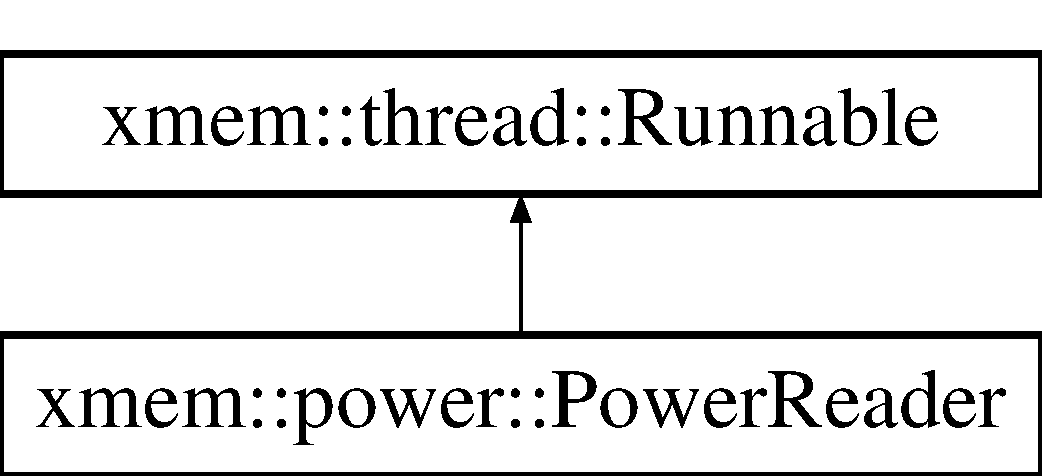
\includegraphics[height=2.000000cm]{classxmem_1_1power_1_1_power_reader}
\end{center}
\end{figure}
\subsection*{Public Member Functions}
\begin{DoxyCompactItemize}
\item 
\hyperlink{classxmem_1_1power_1_1_power_reader_abae158275e32689c1c69a90b8962959b}{Power\-Reader} (double sampling\-\_\-period, double power\-\_\-units, std\-::string \hyperlink{classxmem_1_1power_1_1_power_reader_ac0f465b044512502eb1824f18d60e3e6}{name}, int32\-\_\-t cpu\-\_\-affinity)
\begin{DoxyCompactList}\small\item\em Constructor. \end{DoxyCompactList}\item 
\hypertarget{classxmem_1_1power_1_1_power_reader_ae3c8c415135bfa4b3ba150c2d9b931a3}{\hyperlink{classxmem_1_1power_1_1_power_reader_ae3c8c415135bfa4b3ba150c2d9b931a3}{$\sim$\-Power\-Reader} ()}\label{classxmem_1_1power_1_1_power_reader_ae3c8c415135bfa4b3ba150c2d9b931a3}

\begin{DoxyCompactList}\small\item\em Destructor. \end{DoxyCompactList}\item 
\hypertarget{classxmem_1_1power_1_1_power_reader_ad8286b3727efbcb0ff5049c6594d126a}{virtual void \hyperlink{classxmem_1_1power_1_1_power_reader_ad8286b3727efbcb0ff5049c6594d126a}{run} ()=0}\label{classxmem_1_1power_1_1_power_reader_ad8286b3727efbcb0ff5049c6594d126a}

\begin{DoxyCompactList}\small\item\em Starts measuring power at the rate implied by the sampling\-\_\-period passed in the constructor. Call \hyperlink{classxmem_1_1power_1_1_power_reader_a5c28efc4aece34a5469d067a133920f4}{stop()} to indicate to stop measuring. \end{DoxyCompactList}\item 
bool \hyperlink{classxmem_1_1power_1_1_power_reader_a5c28efc4aece34a5469d067a133920f4}{stop} ()
\begin{DoxyCompactList}\small\item\em Signals to stop measuring power. This is a non-\/blocking call and return does not indicate the measurement has actually stopped. \end{DoxyCompactList}\item 
bool \hyperlink{classxmem_1_1power_1_1_power_reader_a953d6b42a83c8c0b709aa49b994c6803}{calculate\-Metrics} ()
\begin{DoxyCompactList}\small\item\em Calculates the relevant metrics. \end{DoxyCompactList}\item 
bool \hyperlink{classxmem_1_1power_1_1_power_reader_a17b206d91ad607dc6fbcd4f2e0f66684}{clear} ()
\begin{DoxyCompactList}\small\item\em Clears the stored power data. \end{DoxyCompactList}\item 
bool \hyperlink{classxmem_1_1power_1_1_power_reader_a6377973eed59cd99bcb475c17e5cb0f2}{clear\-\_\-and\-\_\-reset} ()
\begin{DoxyCompactList}\small\item\em Clears the stored power data and resets state so that a new thread can be used with this object. \end{DoxyCompactList}\item 
std\-::vector$<$ double $>$ \hyperlink{classxmem_1_1power_1_1_power_reader_af41f0300055c2ec45785cc4e77864a7d}{get\-Power\-Trace} ()
\begin{DoxyCompactList}\small\item\em Gets the power trace. \end{DoxyCompactList}\item 
double \hyperlink{classxmem_1_1power_1_1_power_reader_a2b20b7e6a22dad732cdb166d90fcfe98}{get\-Average\-Power} ()
\begin{DoxyCompactList}\small\item\em Gets the average power. \end{DoxyCompactList}\item 
double \hyperlink{classxmem_1_1power_1_1_power_reader_ae530d62676bd3b3115815b0f4592a0d6}{get\-Peak\-Power} ()
\begin{DoxyCompactList}\small\item\em Gets the peak power. \end{DoxyCompactList}\item 
double \hyperlink{classxmem_1_1power_1_1_power_reader_a0025b83ec146f206257690ef27323141}{get\-Last\-Sample} ()
\begin{DoxyCompactList}\small\item\em Gets the last sample. \end{DoxyCompactList}\item 
double \hyperlink{classxmem_1_1power_1_1_power_reader_a833084fa298a654a7cf589723483399c}{get\-Sampling\-Period} ()
\begin{DoxyCompactList}\small\item\em Gets the sampling period. \end{DoxyCompactList}\item 
double \hyperlink{classxmem_1_1power_1_1_power_reader_a951b1ddd8a39df60b2668548e7529064}{get\-Power\-Units} ()
\begin{DoxyCompactList}\small\item\em Gets the units of samples in watts. \end{DoxyCompactList}\item 
size\-\_\-t \hyperlink{classxmem_1_1power_1_1_power_reader_af35118b0e7d408679497f84aa0f6397e}{get\-Num\-Samples} ()
\begin{DoxyCompactList}\small\item\em Gets the number of samples collected. \end{DoxyCompactList}\item 
std\-::string \hyperlink{classxmem_1_1power_1_1_power_reader_ac0f465b044512502eb1824f18d60e3e6}{name} ()
\begin{DoxyCompactList}\small\item\em Gets the name of this object. \end{DoxyCompactList}\end{DoxyCompactItemize}
\subsection*{Protected Attributes}
\begin{DoxyCompactItemize}
\item 
bool \hyperlink{classxmem_1_1power_1_1_power_reader_a1c0c890279f3f2b7eb41ab3e5889bf2e}{\-\_\-stop\-\_\-signal}
\item 
double \hyperlink{classxmem_1_1power_1_1_power_reader_a2835c933bd4807d6b3133a521dd76641}{\-\_\-power\-\_\-units}
\item 
std\-::string \hyperlink{classxmem_1_1power_1_1_power_reader_a85791da354d03c0a0f7ca4cf38b89e4c}{\-\_\-name}
\item 
int32\-\_\-t \hyperlink{classxmem_1_1power_1_1_power_reader_a0f95e6c4e8caa6db8de3fcf78509e887}{\-\_\-cpu\-\_\-affinity}
\item 
std\-::vector$<$ double $>$ \hyperlink{classxmem_1_1power_1_1_power_reader_ac8ad4bada42912ece1cbb0769dbe3b4d}{\-\_\-power\-\_\-trace}
\item 
double \hyperlink{classxmem_1_1power_1_1_power_reader_a1ad637b79a21519c20f9dda64fc1b908}{\-\_\-average\-\_\-power}
\item 
double \hyperlink{classxmem_1_1power_1_1_power_reader_a0bfe4f56c143f3febb404d85558e45fa}{\-\_\-peak\-\_\-power}
\item 
size\-\_\-t \hyperlink{classxmem_1_1power_1_1_power_reader_a296a8d15083e01e33590cbcd836aa07b}{\-\_\-num\-\_\-samples}
\item 
double \hyperlink{classxmem_1_1power_1_1_power_reader_a1c7d9b505d3c94347c43437a568e5948}{\-\_\-sampling\-\_\-period}
\end{DoxyCompactItemize}
\subsection*{Additional Inherited Members}


\subsection{Detailed Description}
An abstract base class for measuring power from an arbitrary source. This class is runnable using a worker thread. 

\subsection{Constructor \& Destructor Documentation}
\hypertarget{classxmem_1_1power_1_1_power_reader_abae158275e32689c1c69a90b8962959b}{\index{xmem\-::power\-::\-Power\-Reader@{xmem\-::power\-::\-Power\-Reader}!Power\-Reader@{Power\-Reader}}
\index{Power\-Reader@{Power\-Reader}!xmem::power::PowerReader@{xmem\-::power\-::\-Power\-Reader}}
\subsubsection[{Power\-Reader}]{\setlength{\rightskip}{0pt plus 5cm}Power\-Reader\-::\-Power\-Reader (
\begin{DoxyParamCaption}
\item[{double}]{sampling\-\_\-period, }
\item[{double}]{power\-\_\-units, }
\item[{std\-::string}]{name, }
\item[{int32\-\_\-t}]{cpu\-\_\-affinity}
\end{DoxyParamCaption}
)}}\label{classxmem_1_1power_1_1_power_reader_abae158275e32689c1c69a90b8962959b}


Constructor. 


\begin{DoxyParams}{Parameters}
{\em sampling\-\_\-period} & The time between power samples in seconds. \\
\hline
{\em power\-\_\-units} & The power units for each sample in watts. \\
\hline
{\em name} & The human-\/friendly name of this object. \\
\hline
{\em cpu\-\_\-affinity} & The logical C\-P\-U to be used by the thread calling this object's \hyperlink{classxmem_1_1power_1_1_power_reader_ad8286b3727efbcb0ff5049c6594d126a}{run()} method. If negative, any C\-P\-U is O\-K (no affinity). \\
\hline
\end{DoxyParams}


\subsection{Member Function Documentation}
\hypertarget{classxmem_1_1power_1_1_power_reader_a953d6b42a83c8c0b709aa49b994c6803}{\index{xmem\-::power\-::\-Power\-Reader@{xmem\-::power\-::\-Power\-Reader}!calculate\-Metrics@{calculate\-Metrics}}
\index{calculate\-Metrics@{calculate\-Metrics}!xmem::power::PowerReader@{xmem\-::power\-::\-Power\-Reader}}
\subsubsection[{calculate\-Metrics}]{\setlength{\rightskip}{0pt plus 5cm}bool Power\-Reader\-::calculate\-Metrics (
\begin{DoxyParamCaption}
{}
\end{DoxyParamCaption}
)}}\label{classxmem_1_1power_1_1_power_reader_a953d6b42a83c8c0b709aa49b994c6803}


Calculates the relevant metrics. 

\begin{DoxyReturn}{Returns}
True on success. 
\end{DoxyReturn}
\hypertarget{classxmem_1_1power_1_1_power_reader_a17b206d91ad607dc6fbcd4f2e0f66684}{\index{xmem\-::power\-::\-Power\-Reader@{xmem\-::power\-::\-Power\-Reader}!clear@{clear}}
\index{clear@{clear}!xmem::power::PowerReader@{xmem\-::power\-::\-Power\-Reader}}
\subsubsection[{clear}]{\setlength{\rightskip}{0pt plus 5cm}bool Power\-Reader\-::clear (
\begin{DoxyParamCaption}
{}
\end{DoxyParamCaption}
)}}\label{classxmem_1_1power_1_1_power_reader_a17b206d91ad607dc6fbcd4f2e0f66684}


Clears the stored power data. 

\begin{DoxyReturn}{Returns}
True on success. 
\end{DoxyReturn}
\hypertarget{classxmem_1_1power_1_1_power_reader_a6377973eed59cd99bcb475c17e5cb0f2}{\index{xmem\-::power\-::\-Power\-Reader@{xmem\-::power\-::\-Power\-Reader}!clear\-\_\-and\-\_\-reset@{clear\-\_\-and\-\_\-reset}}
\index{clear\-\_\-and\-\_\-reset@{clear\-\_\-and\-\_\-reset}!xmem::power::PowerReader@{xmem\-::power\-::\-Power\-Reader}}
\subsubsection[{clear\-\_\-and\-\_\-reset}]{\setlength{\rightskip}{0pt plus 5cm}bool Power\-Reader\-::clear\-\_\-and\-\_\-reset (
\begin{DoxyParamCaption}
{}
\end{DoxyParamCaption}
)}}\label{classxmem_1_1power_1_1_power_reader_a6377973eed59cd99bcb475c17e5cb0f2}


Clears the stored power data and resets state so that a new thread can be used with this object. 

\begin{DoxyReturn}{Returns}
True on success. 
\end{DoxyReturn}
\hypertarget{classxmem_1_1power_1_1_power_reader_a2b20b7e6a22dad732cdb166d90fcfe98}{\index{xmem\-::power\-::\-Power\-Reader@{xmem\-::power\-::\-Power\-Reader}!get\-Average\-Power@{get\-Average\-Power}}
\index{get\-Average\-Power@{get\-Average\-Power}!xmem::power::PowerReader@{xmem\-::power\-::\-Power\-Reader}}
\subsubsection[{get\-Average\-Power}]{\setlength{\rightskip}{0pt plus 5cm}double Power\-Reader\-::get\-Average\-Power (
\begin{DoxyParamCaption}
{}
\end{DoxyParamCaption}
)}}\label{classxmem_1_1power_1_1_power_reader_a2b20b7e6a22dad732cdb166d90fcfe98}


Gets the average power. 

\begin{DoxyReturn}{Returns}
The average power from the measurements. If no data was collected, returns 0. 
\end{DoxyReturn}
\hypertarget{classxmem_1_1power_1_1_power_reader_a0025b83ec146f206257690ef27323141}{\index{xmem\-::power\-::\-Power\-Reader@{xmem\-::power\-::\-Power\-Reader}!get\-Last\-Sample@{get\-Last\-Sample}}
\index{get\-Last\-Sample@{get\-Last\-Sample}!xmem::power::PowerReader@{xmem\-::power\-::\-Power\-Reader}}
\subsubsection[{get\-Last\-Sample}]{\setlength{\rightskip}{0pt plus 5cm}double Power\-Reader\-::get\-Last\-Sample (
\begin{DoxyParamCaption}
{}
\end{DoxyParamCaption}
)}}\label{classxmem_1_1power_1_1_power_reader_a0025b83ec146f206257690ef27323141}


Gets the last sample. 

\begin{DoxyReturn}{Returns}
The last power sample measured. 
\end{DoxyReturn}
\hypertarget{classxmem_1_1power_1_1_power_reader_af35118b0e7d408679497f84aa0f6397e}{\index{xmem\-::power\-::\-Power\-Reader@{xmem\-::power\-::\-Power\-Reader}!get\-Num\-Samples@{get\-Num\-Samples}}
\index{get\-Num\-Samples@{get\-Num\-Samples}!xmem::power::PowerReader@{xmem\-::power\-::\-Power\-Reader}}
\subsubsection[{get\-Num\-Samples}]{\setlength{\rightskip}{0pt plus 5cm}size\-\_\-t Power\-Reader\-::get\-Num\-Samples (
\begin{DoxyParamCaption}
{}
\end{DoxyParamCaption}
)}}\label{classxmem_1_1power_1_1_power_reader_af35118b0e7d408679497f84aa0f6397e}


Gets the number of samples collected. 

\begin{DoxyReturn}{Returns}
Number of samples collected. 
\end{DoxyReturn}
\hypertarget{classxmem_1_1power_1_1_power_reader_ae530d62676bd3b3115815b0f4592a0d6}{\index{xmem\-::power\-::\-Power\-Reader@{xmem\-::power\-::\-Power\-Reader}!get\-Peak\-Power@{get\-Peak\-Power}}
\index{get\-Peak\-Power@{get\-Peak\-Power}!xmem::power::PowerReader@{xmem\-::power\-::\-Power\-Reader}}
\subsubsection[{get\-Peak\-Power}]{\setlength{\rightskip}{0pt plus 5cm}double Power\-Reader\-::get\-Peak\-Power (
\begin{DoxyParamCaption}
{}
\end{DoxyParamCaption}
)}}\label{classxmem_1_1power_1_1_power_reader_ae530d62676bd3b3115815b0f4592a0d6}


Gets the peak power. 

\begin{DoxyReturn}{Returns}
The peak power sample from the measurements. If no data was collected, returns 0. 
\end{DoxyReturn}
\hypertarget{classxmem_1_1power_1_1_power_reader_af41f0300055c2ec45785cc4e77864a7d}{\index{xmem\-::power\-::\-Power\-Reader@{xmem\-::power\-::\-Power\-Reader}!get\-Power\-Trace@{get\-Power\-Trace}}
\index{get\-Power\-Trace@{get\-Power\-Trace}!xmem::power::PowerReader@{xmem\-::power\-::\-Power\-Reader}}
\subsubsection[{get\-Power\-Trace}]{\setlength{\rightskip}{0pt plus 5cm}std\-::vector$<$ double $>$ Power\-Reader\-::get\-Power\-Trace (
\begin{DoxyParamCaption}
{}
\end{DoxyParamCaption}
)}}\label{classxmem_1_1power_1_1_power_reader_af41f0300055c2ec45785cc4e77864a7d}


Gets the power trace. 

\begin{DoxyReturn}{Returns}
The measured power trace in a vector. If no data was collected, the vector will be empty. 
\end{DoxyReturn}
\hypertarget{classxmem_1_1power_1_1_power_reader_a951b1ddd8a39df60b2668548e7529064}{\index{xmem\-::power\-::\-Power\-Reader@{xmem\-::power\-::\-Power\-Reader}!get\-Power\-Units@{get\-Power\-Units}}
\index{get\-Power\-Units@{get\-Power\-Units}!xmem::power::PowerReader@{xmem\-::power\-::\-Power\-Reader}}
\subsubsection[{get\-Power\-Units}]{\setlength{\rightskip}{0pt plus 5cm}double Power\-Reader\-::get\-Power\-Units (
\begin{DoxyParamCaption}
{}
\end{DoxyParamCaption}
)}}\label{classxmem_1_1power_1_1_power_reader_a951b1ddd8a39df60b2668548e7529064}


Gets the units of samples in watts. 

\begin{DoxyReturn}{Returns}
The power units for each measurement sample in watts. For example, if each measurement is in milliwatts, then this returns 1e-\/3. 
\end{DoxyReturn}
\hypertarget{classxmem_1_1power_1_1_power_reader_a833084fa298a654a7cf589723483399c}{\index{xmem\-::power\-::\-Power\-Reader@{xmem\-::power\-::\-Power\-Reader}!get\-Sampling\-Period@{get\-Sampling\-Period}}
\index{get\-Sampling\-Period@{get\-Sampling\-Period}!xmem::power::PowerReader@{xmem\-::power\-::\-Power\-Reader}}
\subsubsection[{get\-Sampling\-Period}]{\setlength{\rightskip}{0pt plus 5cm}double Power\-Reader\-::get\-Sampling\-Period (
\begin{DoxyParamCaption}
{}
\end{DoxyParamCaption}
)}}\label{classxmem_1_1power_1_1_power_reader_a833084fa298a654a7cf589723483399c}


Gets the sampling period. 

\begin{DoxyReturn}{Returns}
The sampling period of the measurements in seconds. 
\end{DoxyReturn}
\hypertarget{classxmem_1_1power_1_1_power_reader_ac0f465b044512502eb1824f18d60e3e6}{\index{xmem\-::power\-::\-Power\-Reader@{xmem\-::power\-::\-Power\-Reader}!name@{name}}
\index{name@{name}!xmem::power::PowerReader@{xmem\-::power\-::\-Power\-Reader}}
\subsubsection[{name}]{\setlength{\rightskip}{0pt plus 5cm}std\-::string Power\-Reader\-::name (
\begin{DoxyParamCaption}
{}
\end{DoxyParamCaption}
)}}\label{classxmem_1_1power_1_1_power_reader_ac0f465b044512502eb1824f18d60e3e6}


Gets the name of this object. 

\begin{DoxyReturn}{Returns}
The human-\/friendly name of this \hyperlink{classxmem_1_1power_1_1_power_reader}{Power\-Reader}. 
\end{DoxyReturn}
\hypertarget{classxmem_1_1power_1_1_power_reader_a5c28efc4aece34a5469d067a133920f4}{\index{xmem\-::power\-::\-Power\-Reader@{xmem\-::power\-::\-Power\-Reader}!stop@{stop}}
\index{stop@{stop}!xmem::power::PowerReader@{xmem\-::power\-::\-Power\-Reader}}
\subsubsection[{stop}]{\setlength{\rightskip}{0pt plus 5cm}bool Power\-Reader\-::stop (
\begin{DoxyParamCaption}
{}
\end{DoxyParamCaption}
)}}\label{classxmem_1_1power_1_1_power_reader_a5c28efc4aece34a5469d067a133920f4}


Signals to stop measuring power. This is a non-\/blocking call and return does not indicate the measurement has actually stopped. 

\begin{DoxyReturn}{Returns}
True if it successfully signaled a stop. 
\end{DoxyReturn}


\subsection{Member Data Documentation}
\hypertarget{classxmem_1_1power_1_1_power_reader_a1ad637b79a21519c20f9dda64fc1b908}{\index{xmem\-::power\-::\-Power\-Reader@{xmem\-::power\-::\-Power\-Reader}!\-\_\-average\-\_\-power@{\-\_\-average\-\_\-power}}
\index{\-\_\-average\-\_\-power@{\-\_\-average\-\_\-power}!xmem::power::PowerReader@{xmem\-::power\-::\-Power\-Reader}}
\subsubsection[{\-\_\-average\-\_\-power}]{\setlength{\rightskip}{0pt plus 5cm}double xmem\-::power\-::\-Power\-Reader\-::\-\_\-average\-\_\-power\hspace{0.3cm}{\ttfamily [protected]}}}\label{classxmem_1_1power_1_1_power_reader_a1ad637b79a21519c20f9dda64fc1b908}
The average power. \hypertarget{classxmem_1_1power_1_1_power_reader_a0f95e6c4e8caa6db8de3fcf78509e887}{\index{xmem\-::power\-::\-Power\-Reader@{xmem\-::power\-::\-Power\-Reader}!\-\_\-cpu\-\_\-affinity@{\-\_\-cpu\-\_\-affinity}}
\index{\-\_\-cpu\-\_\-affinity@{\-\_\-cpu\-\_\-affinity}!xmem::power::PowerReader@{xmem\-::power\-::\-Power\-Reader}}
\subsubsection[{\-\_\-cpu\-\_\-affinity}]{\setlength{\rightskip}{0pt plus 5cm}int32\-\_\-t xmem\-::power\-::\-Power\-Reader\-::\-\_\-cpu\-\_\-affinity\hspace{0.3cm}{\ttfamily [protected]}}}\label{classxmem_1_1power_1_1_power_reader_a0f95e6c4e8caa6db8de3fcf78509e887}
C\-P\-U affinity for any thread using this object's \hyperlink{classxmem_1_1power_1_1_power_reader_ad8286b3727efbcb0ff5049c6594d126a}{run()} method. If negative, no affinity preference. \hypertarget{classxmem_1_1power_1_1_power_reader_a85791da354d03c0a0f7ca4cf38b89e4c}{\index{xmem\-::power\-::\-Power\-Reader@{xmem\-::power\-::\-Power\-Reader}!\-\_\-name@{\-\_\-name}}
\index{\-\_\-name@{\-\_\-name}!xmem::power::PowerReader@{xmem\-::power\-::\-Power\-Reader}}
\subsubsection[{\-\_\-name}]{\setlength{\rightskip}{0pt plus 5cm}std\-::string xmem\-::power\-::\-Power\-Reader\-::\-\_\-name\hspace{0.3cm}{\ttfamily [protected]}}}\label{classxmem_1_1power_1_1_power_reader_a85791da354d03c0a0f7ca4cf38b89e4c}
Name of this object. \hypertarget{classxmem_1_1power_1_1_power_reader_a296a8d15083e01e33590cbcd836aa07b}{\index{xmem\-::power\-::\-Power\-Reader@{xmem\-::power\-::\-Power\-Reader}!\-\_\-num\-\_\-samples@{\-\_\-num\-\_\-samples}}
\index{\-\_\-num\-\_\-samples@{\-\_\-num\-\_\-samples}!xmem::power::PowerReader@{xmem\-::power\-::\-Power\-Reader}}
\subsubsection[{\-\_\-num\-\_\-samples}]{\setlength{\rightskip}{0pt plus 5cm}size\-\_\-t xmem\-::power\-::\-Power\-Reader\-::\-\_\-num\-\_\-samples\hspace{0.3cm}{\ttfamily [protected]}}}\label{classxmem_1_1power_1_1_power_reader_a296a8d15083e01e33590cbcd836aa07b}
The number of samples collected. \hypertarget{classxmem_1_1power_1_1_power_reader_a0bfe4f56c143f3febb404d85558e45fa}{\index{xmem\-::power\-::\-Power\-Reader@{xmem\-::power\-::\-Power\-Reader}!\-\_\-peak\-\_\-power@{\-\_\-peak\-\_\-power}}
\index{\-\_\-peak\-\_\-power@{\-\_\-peak\-\_\-power}!xmem::power::PowerReader@{xmem\-::power\-::\-Power\-Reader}}
\subsubsection[{\-\_\-peak\-\_\-power}]{\setlength{\rightskip}{0pt plus 5cm}double xmem\-::power\-::\-Power\-Reader\-::\-\_\-peak\-\_\-power\hspace{0.3cm}{\ttfamily [protected]}}}\label{classxmem_1_1power_1_1_power_reader_a0bfe4f56c143f3febb404d85558e45fa}
The peak power observed. \hypertarget{classxmem_1_1power_1_1_power_reader_ac8ad4bada42912ece1cbb0769dbe3b4d}{\index{xmem\-::power\-::\-Power\-Reader@{xmem\-::power\-::\-Power\-Reader}!\-\_\-power\-\_\-trace@{\-\_\-power\-\_\-trace}}
\index{\-\_\-power\-\_\-trace@{\-\_\-power\-\_\-trace}!xmem::power::PowerReader@{xmem\-::power\-::\-Power\-Reader}}
\subsubsection[{\-\_\-power\-\_\-trace}]{\setlength{\rightskip}{0pt plus 5cm}std\-::vector$<$double$>$ xmem\-::power\-::\-Power\-Reader\-::\-\_\-power\-\_\-trace\hspace{0.3cm}{\ttfamily [protected]}}}\label{classxmem_1_1power_1_1_power_reader_ac8ad4bada42912ece1cbb0769dbe3b4d}
The time-\/ordered list of power samples. The first index is the oldest measurement. \hypertarget{classxmem_1_1power_1_1_power_reader_a2835c933bd4807d6b3133a521dd76641}{\index{xmem\-::power\-::\-Power\-Reader@{xmem\-::power\-::\-Power\-Reader}!\-\_\-power\-\_\-units@{\-\_\-power\-\_\-units}}
\index{\-\_\-power\-\_\-units@{\-\_\-power\-\_\-units}!xmem::power::PowerReader@{xmem\-::power\-::\-Power\-Reader}}
\subsubsection[{\-\_\-power\-\_\-units}]{\setlength{\rightskip}{0pt plus 5cm}double xmem\-::power\-::\-Power\-Reader\-::\-\_\-power\-\_\-units\hspace{0.3cm}{\ttfamily [protected]}}}\label{classxmem_1_1power_1_1_power_reader_a2835c933bd4807d6b3133a521dd76641}
Power units in watts. \hypertarget{classxmem_1_1power_1_1_power_reader_a1c7d9b505d3c94347c43437a568e5948}{\index{xmem\-::power\-::\-Power\-Reader@{xmem\-::power\-::\-Power\-Reader}!\-\_\-sampling\-\_\-period@{\-\_\-sampling\-\_\-period}}
\index{\-\_\-sampling\-\_\-period@{\-\_\-sampling\-\_\-period}!xmem::power::PowerReader@{xmem\-::power\-::\-Power\-Reader}}
\subsubsection[{\-\_\-sampling\-\_\-period}]{\setlength{\rightskip}{0pt plus 5cm}double xmem\-::power\-::\-Power\-Reader\-::\-\_\-sampling\-\_\-period\hspace{0.3cm}{\ttfamily [protected]}}}\label{classxmem_1_1power_1_1_power_reader_a1c7d9b505d3c94347c43437a568e5948}
Power sampling period in seconds. \hypertarget{classxmem_1_1power_1_1_power_reader_a1c0c890279f3f2b7eb41ab3e5889bf2e}{\index{xmem\-::power\-::\-Power\-Reader@{xmem\-::power\-::\-Power\-Reader}!\-\_\-stop\-\_\-signal@{\-\_\-stop\-\_\-signal}}
\index{\-\_\-stop\-\_\-signal@{\-\_\-stop\-\_\-signal}!xmem::power::PowerReader@{xmem\-::power\-::\-Power\-Reader}}
\subsubsection[{\-\_\-stop\-\_\-signal}]{\setlength{\rightskip}{0pt plus 5cm}bool xmem\-::power\-::\-Power\-Reader\-::\-\_\-stop\-\_\-signal\hspace{0.3cm}{\ttfamily [protected]}}}\label{classxmem_1_1power_1_1_power_reader_a1c0c890279f3f2b7eb41ab3e5889bf2e}
When true, the \hyperlink{classxmem_1_1power_1_1_power_reader_ad8286b3727efbcb0ff5049c6594d126a}{run()} function should finish after the current sample iteration it is working on. 

The documentation for this class was generated from the following files\-:\begin{DoxyCompactItemize}
\item 
src/include/\hyperlink{_power_reader_8h}{Power\-Reader.\-h}\item 
src/\hyperlink{_power_reader_8cpp}{Power\-Reader.\-cpp}\end{DoxyCompactItemize}

\hypertarget{structxmem_1_1config_1_1third__party_1_1_print_usage_implementation}{}\section{xmem\+:\+:config\+:\+:third\+\_\+party\+:\+:Print\+Usage\+Implementation Struct Reference}
\label{structxmem_1_1config_1_1third__party_1_1_print_usage_implementation}\index{xmem\+::config\+::third\+\_\+party\+::\+Print\+Usage\+Implementation@{xmem\+::config\+::third\+\_\+party\+::\+Print\+Usage\+Implementation}}
\subsection*{Classes}
\begin{DoxyCompactItemize}
\item 
struct \hyperlink{structxmem_1_1config_1_1third__party_1_1_print_usage_implementation_1_1_function_writer}{Function\+Writer}
\item 
struct \hyperlink{structxmem_1_1config_1_1third__party_1_1_print_usage_implementation_1_1_i_string_writer}{I\+String\+Writer}
\item 
class \hyperlink{classxmem_1_1config_1_1third__party_1_1_print_usage_implementation_1_1_line_part_iterator}{Line\+Part\+Iterator}
\item 
class \hyperlink{classxmem_1_1config_1_1third__party_1_1_print_usage_implementation_1_1_line_wrapper}{Line\+Wrapper}
\item 
struct \hyperlink{structxmem_1_1config_1_1third__party_1_1_print_usage_implementation_1_1_o_stream_writer}{O\+Stream\+Writer}
\item 
struct \hyperlink{structxmem_1_1config_1_1third__party_1_1_print_usage_implementation_1_1_stream_writer}{Stream\+Writer}
\item 
struct \hyperlink{structxmem_1_1config_1_1third__party_1_1_print_usage_implementation_1_1_syscall_writer}{Syscall\+Writer}
\item 
struct \hyperlink{structxmem_1_1config_1_1third__party_1_1_print_usage_implementation_1_1_temporary_writer}{Temporary\+Writer}
\end{DoxyCompactItemize}
\subsection*{Static Public Member Functions}
\begin{DoxyCompactItemize}
\item 
\hypertarget{structxmem_1_1config_1_1third__party_1_1_print_usage_implementation_a61c94ce9b05817ba381f67c876c31317}{}static void {\bfseries upmax} (int \&i1, int i2)\label{structxmem_1_1config_1_1third__party_1_1_print_usage_implementation_a61c94ce9b05817ba381f67c876c31317}

\item 
\hypertarget{structxmem_1_1config_1_1third__party_1_1_print_usage_implementation_a9282ea42ec7d06c6150b3b5e184c0916}{}static void {\bfseries indent} (\hyperlink{structxmem_1_1config_1_1third__party_1_1_print_usage_implementation_1_1_i_string_writer}{I\+String\+Writer} \&write, int \&x, int want\+\_\+x)\label{structxmem_1_1config_1_1third__party_1_1_print_usage_implementation_a9282ea42ec7d06c6150b3b5e184c0916}

\item 
static bool \hyperlink{structxmem_1_1config_1_1third__party_1_1_print_usage_implementation_a26b1905c90b5ccc4e8f1db6b5646fc6f}{is\+Wide\+Char} (unsigned ch)
\begin{DoxyCompactList}\small\item\em Returns true if ch is the unicode code point of a wide character. \end{DoxyCompactList}\item 
\hypertarget{structxmem_1_1config_1_1third__party_1_1_print_usage_implementation_ab74ee659e276695044e9fb4312c3cef9}{}static void {\bfseries print\+Usage} (\hyperlink{structxmem_1_1config_1_1third__party_1_1_print_usage_implementation_1_1_i_string_writer}{I\+String\+Writer} \&write, const \hyperlink{structxmem_1_1config_1_1third__party_1_1_descriptor}{Descriptor} usage\mbox{[}$\,$\mbox{]}, int width=80, int last\+\_\+column\+\_\+min\+\_\+percent=50, int last\+\_\+column\+\_\+own\+\_\+line\+\_\+max\+\_\+percent=75)\label{structxmem_1_1config_1_1third__party_1_1_print_usage_implementation_ab74ee659e276695044e9fb4312c3cef9}

\end{DoxyCompactItemize}


\subsection{Member Function Documentation}
\hypertarget{structxmem_1_1config_1_1third__party_1_1_print_usage_implementation_a26b1905c90b5ccc4e8f1db6b5646fc6f}{}\index{xmem\+::config\+::third\+\_\+party\+::\+Print\+Usage\+Implementation@{xmem\+::config\+::third\+\_\+party\+::\+Print\+Usage\+Implementation}!is\+Wide\+Char@{is\+Wide\+Char}}
\index{is\+Wide\+Char@{is\+Wide\+Char}!xmem\+::config\+::third\+\_\+party\+::\+Print\+Usage\+Implementation@{xmem\+::config\+::third\+\_\+party\+::\+Print\+Usage\+Implementation}}
\subsubsection[{is\+Wide\+Char}]{\setlength{\rightskip}{0pt plus 5cm}static bool xmem\+::config\+::third\+\_\+party\+::\+Print\+Usage\+Implementation\+::is\+Wide\+Char (
\begin{DoxyParamCaption}
\item[{unsigned}]{ch}
\end{DoxyParamCaption}
)\hspace{0.3cm}{\ttfamily [inline]}, {\ttfamily [static]}}\label{structxmem_1_1config_1_1third__party_1_1_print_usage_implementation_a26b1905c90b5ccc4e8f1db6b5646fc6f}


Returns true if ch is the unicode code point of a wide character. 

\begin{DoxyNote}{Note}
The following character ranges are treated as wide 
\begin{DoxyCode}
1100..115F
2329..232A  (just 2 characters!)
2E80..A4C6  except \textcolor{keywordflow}{for} 303F
A960..A97C
AC00..D7FB
F900..FAFF
FE10..FE6B
FF01..FF60
FFE0..FFE6
1B000......
\end{DoxyCode}
 
\end{DoxyNote}


The documentation for this struct was generated from the following file\+:\begin{DoxyCompactItemize}
\item 
src/include/\hyperlink{optionparser_8h}{optionparser.\+h}\end{DoxyCompactItemize}

\hypertarget{classxmem_1_1timers_1_1win_1_1_q_p_c_timer}{}\section{xmem\+:\+:timers\+:\+:win\+:\+:Q\+P\+C\+Timer Class Reference}
\label{classxmem_1_1timers_1_1win_1_1_q_p_c_timer}\index{xmem\+::timers\+::win\+::\+Q\+P\+C\+Timer@{xmem\+::timers\+::win\+::\+Q\+P\+C\+Timer}}


This class implements a simple high resolution stopwatch timer based on Windows\textquotesingle{} Query\+Performance\+Counter A\+P\+I. W\+A\+R\+N\+I\+N\+G\+: these objects are N\+O\+T thread safe.  




{\ttfamily \#include $<$Q\+P\+C\+Timer.\+h$>$}

Inheritance diagram for xmem\+:\+:timers\+:\+:win\+:\+:Q\+P\+C\+Timer\+:\begin{figure}[H]
\begin{center}
\leavevmode
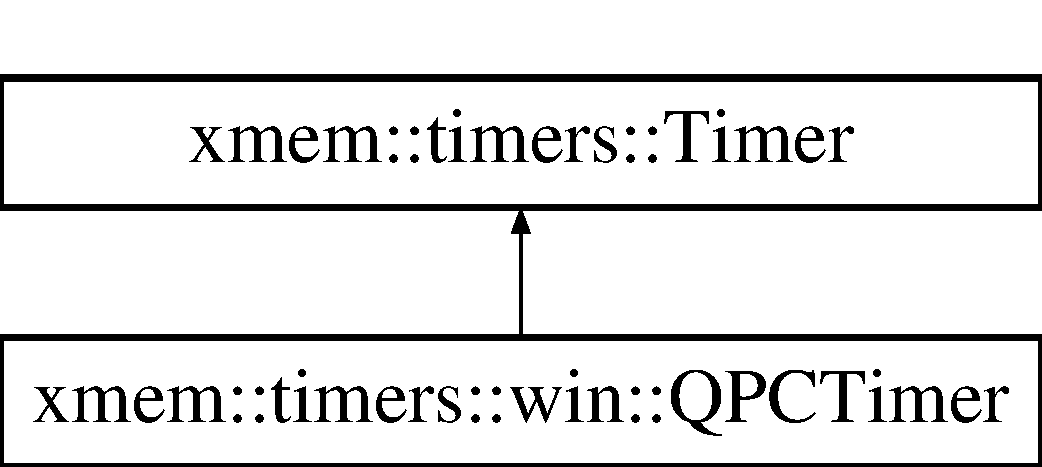
\includegraphics[height=2.000000cm]{classxmem_1_1timers_1_1win_1_1_q_p_c_timer}
\end{center}
\end{figure}
\subsection*{Public Member Functions}
\begin{DoxyCompactItemize}
\item 
\hypertarget{classxmem_1_1timers_1_1win_1_1_q_p_c_timer_a4f05ac32e4c2fd981e84646de2de526e}{}\hyperlink{classxmem_1_1timers_1_1win_1_1_q_p_c_timer_a4f05ac32e4c2fd981e84646de2de526e}{Q\+P\+C\+Timer} ()\label{classxmem_1_1timers_1_1win_1_1_q_p_c_timer_a4f05ac32e4c2fd981e84646de2de526e}

\begin{DoxyCompactList}\small\item\em Constructor. This may take a noticeable amount of time. \end{DoxyCompactList}\item 
\hypertarget{classxmem_1_1timers_1_1win_1_1_q_p_c_timer_a22e88913a13a0d543d18ffcaec7c0466}{}virtual void \hyperlink{classxmem_1_1timers_1_1win_1_1_q_p_c_timer_a22e88913a13a0d543d18ffcaec7c0466}{start} ()\label{classxmem_1_1timers_1_1win_1_1_q_p_c_timer_a22e88913a13a0d543d18ffcaec7c0466}

\begin{DoxyCompactList}\small\item\em Starts the timer. \end{DoxyCompactList}\item 
virtual uint64\+\_\+t \hyperlink{classxmem_1_1timers_1_1win_1_1_q_p_c_timer_a22ef37cd945c7e57345e1ce83340884a}{stop} ()
\begin{DoxyCompactList}\small\item\em Stops the timer. \end{DoxyCompactList}\end{DoxyCompactItemize}
\subsection*{Additional Inherited Members}


\subsection{Detailed Description}
This class implements a simple high resolution stopwatch timer based on Windows\textquotesingle{} Query\+Performance\+Counter A\+P\+I. W\+A\+R\+N\+I\+N\+G\+: these objects are N\+O\+T thread safe. 

\subsection{Member Function Documentation}
\hypertarget{classxmem_1_1timers_1_1win_1_1_q_p_c_timer_a22ef37cd945c7e57345e1ce83340884a}{}\index{xmem\+::timers\+::win\+::\+Q\+P\+C\+Timer@{xmem\+::timers\+::win\+::\+Q\+P\+C\+Timer}!stop@{stop}}
\index{stop@{stop}!xmem\+::timers\+::win\+::\+Q\+P\+C\+Timer@{xmem\+::timers\+::win\+::\+Q\+P\+C\+Timer}}
\subsubsection[{stop}]{\setlength{\rightskip}{0pt plus 5cm}uint64\+\_\+t Q\+P\+C\+Timer\+::stop (
\begin{DoxyParamCaption}
{}
\end{DoxyParamCaption}
)\hspace{0.3cm}{\ttfamily [virtual]}}\label{classxmem_1_1timers_1_1win_1_1_q_p_c_timer_a22ef37cd945c7e57345e1ce83340884a}


Stops the timer. 

\begin{DoxyReturn}{Returns}
Elapsed time since last \hyperlink{classxmem_1_1timers_1_1win_1_1_q_p_c_timer_a22e88913a13a0d543d18ffcaec7c0466}{start()} call in ticks. 
\end{DoxyReturn}


Implements \hyperlink{classxmem_1_1timers_1_1_timer_a3be174c5eb733a2974ce76c146874e1f}{xmem\+::timers\+::\+Timer}.



The documentation for this class was generated from the following files\+:\begin{DoxyCompactItemize}
\item 
src/include/win/\hyperlink{_q_p_c_timer_8h}{Q\+P\+C\+Timer.\+h}\item 
src/win/\hyperlink{_q_p_c_timer_8cpp}{Q\+P\+C\+Timer.\+cpp}\end{DoxyCompactItemize}

\hypertarget{classxmem_1_1thread_1_1_runnable}{}\section{xmem\+:\+:thread\+:\+:Runnable Class Reference}
\label{classxmem_1_1thread_1_1_runnable}\index{xmem\+::thread\+::\+Runnable@{xmem\+::thread\+::\+Runnable}}


A base class for any object that implements a thread-\/safe \hyperlink{classxmem_1_1thread_1_1_runnable_af2915224b03db20403550291672733a7}{run()} function for use by \hyperlink{classxmem_1_1thread_1_1_thread}{Thread} objects.  




{\ttfamily \#include $<$Runnable.\+h$>$}

Inheritance diagram for xmem\+:\+:thread\+:\+:Runnable\+:\begin{figure}[H]
\begin{center}
\leavevmode
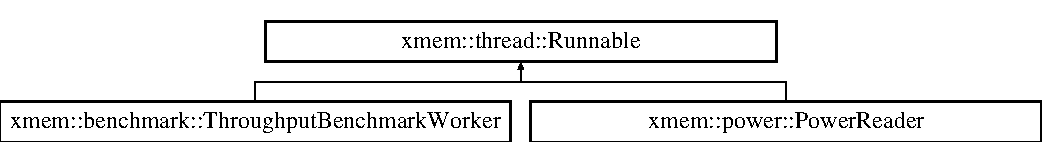
\includegraphics[height=1.911263cm]{classxmem_1_1thread_1_1_runnable}
\end{center}
\end{figure}
\subsection*{Public Member Functions}
\begin{DoxyCompactItemize}
\item 
\hypertarget{classxmem_1_1thread_1_1_runnable_a19af0a2e2b8f986c51196b9c4b2340fb}{}\hyperlink{classxmem_1_1thread_1_1_runnable_a19af0a2e2b8f986c51196b9c4b2340fb}{Runnable} ()\label{classxmem_1_1thread_1_1_runnable_a19af0a2e2b8f986c51196b9c4b2340fb}

\begin{DoxyCompactList}\small\item\em Constructor. \end{DoxyCompactList}\item 
\hypertarget{classxmem_1_1thread_1_1_runnable_a3bf7483afb8d40ec8dbec57efb64f0c2}{}\hyperlink{classxmem_1_1thread_1_1_runnable_a3bf7483afb8d40ec8dbec57efb64f0c2}{$\sim$\+Runnable} ()\label{classxmem_1_1thread_1_1_runnable_a3bf7483afb8d40ec8dbec57efb64f0c2}

\begin{DoxyCompactList}\small\item\em Destructor. \end{DoxyCompactList}\item 
\hypertarget{classxmem_1_1thread_1_1_runnable_af2915224b03db20403550291672733a7}{}virtual void \hyperlink{classxmem_1_1thread_1_1_runnable_af2915224b03db20403550291672733a7}{run} ()=0\label{classxmem_1_1thread_1_1_runnable_af2915224b03db20403550291672733a7}

\begin{DoxyCompactList}\small\item\em Does some \char`\"{}work\char`\"{}. Pure virtual method that any derived class must implement in a thread-\/safe manner. \end{DoxyCompactList}\end{DoxyCompactItemize}
\subsection*{Protected Member Functions}
\begin{DoxyCompactItemize}
\item 
bool \hyperlink{classxmem_1_1thread_1_1_runnable_ad2a24a9e69f4592ceb1356d28d45f784}{\+\_\+acquire\+Lock} (int32\+\_\+t timeout)
\begin{DoxyCompactList}\small\item\em Acquires the object lock to access all object state in thread-\/safe manner. \end{DoxyCompactList}\item 
bool \hyperlink{classxmem_1_1thread_1_1_runnable_aacef5cf385638157e24e7a33d0a4e450}{\+\_\+release\+Lock} ()
\begin{DoxyCompactList}\small\item\em Releases the object lock to access all object state in thread-\/safe manner. \end{DoxyCompactList}\end{DoxyCompactItemize}


\subsection{Detailed Description}
A base class for any object that implements a thread-\/safe \hyperlink{classxmem_1_1thread_1_1_runnable_af2915224b03db20403550291672733a7}{run()} function for use by \hyperlink{classxmem_1_1thread_1_1_thread}{Thread} objects. 

\subsection{Member Function Documentation}
\hypertarget{classxmem_1_1thread_1_1_runnable_ad2a24a9e69f4592ceb1356d28d45f784}{}\index{xmem\+::thread\+::\+Runnable@{xmem\+::thread\+::\+Runnable}!\+\_\+acquire\+Lock@{\+\_\+acquire\+Lock}}
\index{\+\_\+acquire\+Lock@{\+\_\+acquire\+Lock}!xmem\+::thread\+::\+Runnable@{xmem\+::thread\+::\+Runnable}}
\subsubsection[{\+\_\+acquire\+Lock}]{\setlength{\rightskip}{0pt plus 5cm}bool Runnable\+::\+\_\+acquire\+Lock (
\begin{DoxyParamCaption}
\item[{int32\+\_\+t}]{timeout}
\end{DoxyParamCaption}
)\hspace{0.3cm}{\ttfamily [protected]}}\label{classxmem_1_1thread_1_1_runnable_ad2a24a9e69f4592ceb1356d28d45f784}


Acquires the object lock to access all object state in thread-\/safe manner. 


\begin{DoxyParams}{Parameters}
{\em timeout} & timeout in milliseconds to acquire the lock. If 0, does not wait at all. If negative, waits indefinitely. \\
\hline
\end{DoxyParams}
\begin{DoxyReturn}{Returns}
true on success. If not successful, the lock was not acquired, possibly due to a timeout, or the lock might already be held. 
\end{DoxyReturn}
\hypertarget{classxmem_1_1thread_1_1_runnable_aacef5cf385638157e24e7a33d0a4e450}{}\index{xmem\+::thread\+::\+Runnable@{xmem\+::thread\+::\+Runnable}!\+\_\+release\+Lock@{\+\_\+release\+Lock}}
\index{\+\_\+release\+Lock@{\+\_\+release\+Lock}!xmem\+::thread\+::\+Runnable@{xmem\+::thread\+::\+Runnable}}
\subsubsection[{\+\_\+release\+Lock}]{\setlength{\rightskip}{0pt plus 5cm}bool Runnable\+::\+\_\+release\+Lock (
\begin{DoxyParamCaption}
{}
\end{DoxyParamCaption}
)\hspace{0.3cm}{\ttfamily [protected]}}\label{classxmem_1_1thread_1_1_runnable_aacef5cf385638157e24e7a33d0a4e450}


Releases the object lock to access all object state in thread-\/safe manner. 

\begin{DoxyReturn}{Returns}
true on success. If not successful, the lock is either still held or the call was illegal (e.\+g., releasing a lock that was never acquired). 
\end{DoxyReturn}


The documentation for this class was generated from the following files\+:\begin{DoxyCompactItemize}
\item 
src/include/\hyperlink{_runnable_8h}{Runnable.\+h}\item 
src/\hyperlink{_runnable_8cpp}{Runnable.\+cpp}\end{DoxyCompactItemize}

\hypertarget{structxmem_1_1config_1_1third__party_1_1_stats}{\section{xmem\-:\-:config\-:\-:third\-\_\-party\-:\-:Stats Struct Reference}
\label{structxmem_1_1config_1_1third__party_1_1_stats}\index{xmem\-::config\-::third\-\_\-party\-::\-Stats@{xmem\-::config\-::third\-\_\-party\-::\-Stats}}
}


Determines the minimum lengths of the buffer and options arrays used for \hyperlink{classxmem_1_1config_1_1third__party_1_1_parser}{Parser}.  




{\ttfamily \#include $<$optionparser.\-h$>$}

\subsection*{Classes}
\begin{DoxyCompactItemize}
\item 
class \hyperlink{classxmem_1_1config_1_1third__party_1_1_stats_1_1_count_options_action}{Count\-Options\-Action}
\end{DoxyCompactItemize}
\subsection*{Public Member Functions}
\begin{DoxyCompactItemize}
\item 
\hypertarget{structxmem_1_1config_1_1third__party_1_1_stats_a355906c24df069815644562a3d91e222}{\hyperlink{structxmem_1_1config_1_1third__party_1_1_stats_a355906c24df069815644562a3d91e222}{Stats} ()}\label{structxmem_1_1config_1_1third__party_1_1_stats_a355906c24df069815644562a3d91e222}

\begin{DoxyCompactList}\small\item\em Creates a \hyperlink{structxmem_1_1config_1_1third__party_1_1_stats}{Stats} object with counts set to 1 (for the sentinel element). \end{DoxyCompactList}\item 
\hyperlink{structxmem_1_1config_1_1third__party_1_1_stats_a3f7d20676c26797e4699d4ed73ab2f40}{Stats} (bool gnu, const \hyperlink{structxmem_1_1config_1_1third__party_1_1_descriptor}{Descriptor} usage\mbox{[}$\,$\mbox{]}, int argc, const char $\ast$$\ast$argv, int min\-\_\-abbr\-\_\-len=0, bool single\-\_\-minus\-\_\-longopt=false)
\begin{DoxyCompactList}\small\item\em Creates a new \hyperlink{structxmem_1_1config_1_1third__party_1_1_stats}{Stats} object and immediately updates it for the given {\ttfamily usage} and argument vector. You may pass 0 for {\ttfamily argc} and/or {\ttfamily argv}, if you just want to update \hyperlink{structxmem_1_1config_1_1third__party_1_1_stats_a74f645c06ae7eab5058f2a51226c2dcd}{options\-\_\-max}. \end{DoxyCompactList}\item 
\hypertarget{structxmem_1_1config_1_1third__party_1_1_stats_ab52b9c9733f95a46ca91ca83acef51eb}{\hyperlink{structxmem_1_1config_1_1third__party_1_1_stats_ab52b9c9733f95a46ca91ca83acef51eb}{Stats} (bool gnu, const \hyperlink{structxmem_1_1config_1_1third__party_1_1_descriptor}{Descriptor} usage\mbox{[}$\,$\mbox{]}, int argc, char $\ast$$\ast$argv, int min\-\_\-abbr\-\_\-len=0, bool single\-\_\-minus\-\_\-longopt=false)}\label{structxmem_1_1config_1_1third__party_1_1_stats_ab52b9c9733f95a46ca91ca83acef51eb}

\begin{DoxyCompactList}\small\item\em \hyperlink{structxmem_1_1config_1_1third__party_1_1_stats}{Stats}(...) with non-\/const argv. \end{DoxyCompactList}\item 
\hypertarget{structxmem_1_1config_1_1third__party_1_1_stats_ab0afa2b202f331e145ffeb5b04518b99}{\hyperlink{structxmem_1_1config_1_1third__party_1_1_stats_ab0afa2b202f331e145ffeb5b04518b99}{Stats} (const \hyperlink{structxmem_1_1config_1_1third__party_1_1_descriptor}{Descriptor} usage\mbox{[}$\,$\mbox{]}, int argc, const char $\ast$$\ast$argv, int min\-\_\-abbr\-\_\-len=0, bool single\-\_\-minus\-\_\-longopt=false)}\label{structxmem_1_1config_1_1third__party_1_1_stats_ab0afa2b202f331e145ffeb5b04518b99}

\begin{DoxyCompactList}\small\item\em P\-O\-S\-I\-X \hyperlink{structxmem_1_1config_1_1third__party_1_1_stats}{Stats}(...) (gnu==false). \end{DoxyCompactList}\item 
\hypertarget{structxmem_1_1config_1_1third__party_1_1_stats_a66177fd0195cf96ed8d8020acc91ead2}{\hyperlink{structxmem_1_1config_1_1third__party_1_1_stats_a66177fd0195cf96ed8d8020acc91ead2}{Stats} (const \hyperlink{structxmem_1_1config_1_1third__party_1_1_descriptor}{Descriptor} usage\mbox{[}$\,$\mbox{]}, int argc, char $\ast$$\ast$argv, int min\-\_\-abbr\-\_\-len=0, bool single\-\_\-minus\-\_\-longopt=false)}\label{structxmem_1_1config_1_1third__party_1_1_stats_a66177fd0195cf96ed8d8020acc91ead2}

\begin{DoxyCompactList}\small\item\em P\-O\-S\-I\-X \hyperlink{structxmem_1_1config_1_1third__party_1_1_stats}{Stats}(...) (gnu==false) with non-\/const argv. \end{DoxyCompactList}\item 
void \hyperlink{structxmem_1_1config_1_1third__party_1_1_stats_a067da76c0d531c9cceb5fd1c3b8c6a2b}{add} (bool gnu, const \hyperlink{structxmem_1_1config_1_1third__party_1_1_descriptor}{Descriptor} usage\mbox{[}$\,$\mbox{]}, int argc, const char $\ast$$\ast$argv, int min\-\_\-abbr\-\_\-len=0, bool single\-\_\-minus\-\_\-longopt=false)
\begin{DoxyCompactList}\small\item\em Updates this \hyperlink{structxmem_1_1config_1_1third__party_1_1_stats}{Stats} object for the given {\ttfamily usage} and argument vector. You may pass 0 for {\ttfamily argc} and/or {\ttfamily argv}, if you just want to update \hyperlink{structxmem_1_1config_1_1third__party_1_1_stats_a74f645c06ae7eab5058f2a51226c2dcd}{options\-\_\-max}. \end{DoxyCompactList}\item 
\hypertarget{structxmem_1_1config_1_1third__party_1_1_stats_af0f264fbbf6fa2c83d56d87c501a8e89}{void \hyperlink{structxmem_1_1config_1_1third__party_1_1_stats_af0f264fbbf6fa2c83d56d87c501a8e89}{add} (bool gnu, const \hyperlink{structxmem_1_1config_1_1third__party_1_1_descriptor}{Descriptor} usage\mbox{[}$\,$\mbox{]}, int argc, char $\ast$$\ast$argv, int min\-\_\-abbr\-\_\-len=0, bool single\-\_\-minus\-\_\-longopt=false)}\label{structxmem_1_1config_1_1third__party_1_1_stats_af0f264fbbf6fa2c83d56d87c501a8e89}

\begin{DoxyCompactList}\small\item\em \hyperlink{structxmem_1_1config_1_1third__party_1_1_stats_a067da76c0d531c9cceb5fd1c3b8c6a2b}{add()} with non-\/const argv. \end{DoxyCompactList}\item 
\hypertarget{structxmem_1_1config_1_1third__party_1_1_stats_aa19ac2a7dda954c719d4de88b8bebe61}{void \hyperlink{structxmem_1_1config_1_1third__party_1_1_stats_aa19ac2a7dda954c719d4de88b8bebe61}{add} (const \hyperlink{structxmem_1_1config_1_1third__party_1_1_descriptor}{Descriptor} usage\mbox{[}$\,$\mbox{]}, int argc, const char $\ast$$\ast$argv, int min\-\_\-abbr\-\_\-len=0, bool single\-\_\-minus\-\_\-longopt=false)}\label{structxmem_1_1config_1_1third__party_1_1_stats_aa19ac2a7dda954c719d4de88b8bebe61}

\begin{DoxyCompactList}\small\item\em P\-O\-S\-I\-X \hyperlink{structxmem_1_1config_1_1third__party_1_1_stats_a067da76c0d531c9cceb5fd1c3b8c6a2b}{add()} (gnu==false). \end{DoxyCompactList}\item 
\hypertarget{structxmem_1_1config_1_1third__party_1_1_stats_a9168980abd6cfd4c2f6fd9d8dbfa9910}{void \hyperlink{structxmem_1_1config_1_1third__party_1_1_stats_a9168980abd6cfd4c2f6fd9d8dbfa9910}{add} (const \hyperlink{structxmem_1_1config_1_1third__party_1_1_descriptor}{Descriptor} usage\mbox{[}$\,$\mbox{]}, int argc, char $\ast$$\ast$argv, int min\-\_\-abbr\-\_\-len=0, bool single\-\_\-minus\-\_\-longopt=false)}\label{structxmem_1_1config_1_1third__party_1_1_stats_a9168980abd6cfd4c2f6fd9d8dbfa9910}

\begin{DoxyCompactList}\small\item\em P\-O\-S\-I\-X \hyperlink{structxmem_1_1config_1_1third__party_1_1_stats_a067da76c0d531c9cceb5fd1c3b8c6a2b}{add()} (gnu==false) with non-\/const argv. \end{DoxyCompactList}\end{DoxyCompactItemize}
\subsection*{Public Attributes}
\begin{DoxyCompactItemize}
\item 
unsigned \hyperlink{structxmem_1_1config_1_1third__party_1_1_stats_a42c3ec9a6baf2c24d783b00279266298}{buffer\-\_\-max}
\begin{DoxyCompactList}\small\item\em Number of elements needed for a {\ttfamily buffer}\mbox{[}\mbox{]} array to be used for \hyperlink{classxmem_1_1config_1_1third__party_1_1_parser_a0e45d97675bc5d003ef6f68ac8cd7249}{parsing} the same argument vectors that were fed into this \hyperlink{structxmem_1_1config_1_1third__party_1_1_stats}{Stats} object. \end{DoxyCompactList}\item 
unsigned \hyperlink{structxmem_1_1config_1_1third__party_1_1_stats_a74f645c06ae7eab5058f2a51226c2dcd}{options\-\_\-max}
\begin{DoxyCompactList}\small\item\em Number of elements needed for an {\ttfamily options}\mbox{[}\mbox{]} array to be used for \hyperlink{classxmem_1_1config_1_1third__party_1_1_parser_a0e45d97675bc5d003ef6f68ac8cd7249}{parsing} the same argument vectors that were fed into this \hyperlink{structxmem_1_1config_1_1third__party_1_1_stats}{Stats} object. \end{DoxyCompactList}\end{DoxyCompactItemize}


\subsection{Detailed Description}
Determines the minimum lengths of the buffer and options arrays used for \hyperlink{classxmem_1_1config_1_1third__party_1_1_parser}{Parser}. 

Because \hyperlink{classxmem_1_1config_1_1third__party_1_1_parser}{Parser} doesn't use dynamic memory its output arrays have to be pre-\/allocated. If you don't want to use fixed size arrays (which may turn out too small, causing command line arguments to be dropped), you can use \hyperlink{structxmem_1_1config_1_1third__party_1_1_stats}{Stats} to determine the correct sizes. \hyperlink{structxmem_1_1config_1_1third__party_1_1_stats}{Stats} work cumulative. You can first pass in your default options and then the real options and afterwards the counts will reflect the union. 

\subsection{Constructor \& Destructor Documentation}
\hypertarget{structxmem_1_1config_1_1third__party_1_1_stats_a3f7d20676c26797e4699d4ed73ab2f40}{\index{xmem\-::config\-::third\-\_\-party\-::\-Stats@{xmem\-::config\-::third\-\_\-party\-::\-Stats}!Stats@{Stats}}
\index{Stats@{Stats}!xmem::config::third_party::Stats@{xmem\-::config\-::third\-\_\-party\-::\-Stats}}
\subsubsection[{Stats}]{\setlength{\rightskip}{0pt plus 5cm}xmem\-::config\-::third\-\_\-party\-::\-Stats\-::\-Stats (
\begin{DoxyParamCaption}
\item[{bool}]{gnu, }
\item[{const {\bf Descriptor}}]{usage\mbox{[}$\,$\mbox{]}, }
\item[{int}]{argc, }
\item[{const char $\ast$$\ast$}]{argv, }
\item[{int}]{min\-\_\-abbr\-\_\-len = {\ttfamily 0}, }
\item[{bool}]{single\-\_\-minus\-\_\-longopt = {\ttfamily false}}
\end{DoxyParamCaption}
)\hspace{0.3cm}{\ttfamily [inline]}}}\label{structxmem_1_1config_1_1third__party_1_1_stats_a3f7d20676c26797e4699d4ed73ab2f40}


Creates a new \hyperlink{structxmem_1_1config_1_1third__party_1_1_stats}{Stats} object and immediately updates it for the given {\ttfamily usage} and argument vector. You may pass 0 for {\ttfamily argc} and/or {\ttfamily argv}, if you just want to update \hyperlink{structxmem_1_1config_1_1third__party_1_1_stats_a74f645c06ae7eab5058f2a51226c2dcd}{options\-\_\-max}. 

\begin{DoxyNote}{Note}
The calls to \hyperlink{structxmem_1_1config_1_1third__party_1_1_stats}{Stats} methods must match the later calls to \hyperlink{classxmem_1_1config_1_1third__party_1_1_parser}{Parser} methods. See \hyperlink{classxmem_1_1config_1_1third__party_1_1_parser_a0e45d97675bc5d003ef6f68ac8cd7249}{Parser\-::parse()} for the meaning of the arguments. 
\end{DoxyNote}


\subsection{Member Function Documentation}
\hypertarget{structxmem_1_1config_1_1third__party_1_1_stats_a067da76c0d531c9cceb5fd1c3b8c6a2b}{\index{xmem\-::config\-::third\-\_\-party\-::\-Stats@{xmem\-::config\-::third\-\_\-party\-::\-Stats}!add@{add}}
\index{add@{add}!xmem::config::third_party::Stats@{xmem\-::config\-::third\-\_\-party\-::\-Stats}}
\subsubsection[{add}]{\setlength{\rightskip}{0pt plus 5cm}void xmem\-::config\-::third\-\_\-party\-::\-Stats\-::add (
\begin{DoxyParamCaption}
\item[{bool}]{gnu, }
\item[{const {\bf Descriptor}}]{usage\mbox{[}$\,$\mbox{]}, }
\item[{int}]{argc, }
\item[{const char $\ast$$\ast$}]{argv, }
\item[{int}]{min\-\_\-abbr\-\_\-len = {\ttfamily 0}, }
\item[{bool}]{single\-\_\-minus\-\_\-longopt = {\ttfamily false}}
\end{DoxyParamCaption}
)\hspace{0.3cm}{\ttfamily [inline]}}}\label{structxmem_1_1config_1_1third__party_1_1_stats_a067da76c0d531c9cceb5fd1c3b8c6a2b}


Updates this \hyperlink{structxmem_1_1config_1_1third__party_1_1_stats}{Stats} object for the given {\ttfamily usage} and argument vector. You may pass 0 for {\ttfamily argc} and/or {\ttfamily argv}, if you just want to update \hyperlink{structxmem_1_1config_1_1third__party_1_1_stats_a74f645c06ae7eab5058f2a51226c2dcd}{options\-\_\-max}. 

\begin{DoxyNote}{Note}
The calls to \hyperlink{structxmem_1_1config_1_1third__party_1_1_stats}{Stats} methods must match the later calls to \hyperlink{classxmem_1_1config_1_1third__party_1_1_parser}{Parser} methods. See \hyperlink{classxmem_1_1config_1_1third__party_1_1_parser_a0e45d97675bc5d003ef6f68ac8cd7249}{Parser\-::parse()} for the meaning of the arguments. 
\end{DoxyNote}


\subsection{Member Data Documentation}
\hypertarget{structxmem_1_1config_1_1third__party_1_1_stats_a42c3ec9a6baf2c24d783b00279266298}{\index{xmem\-::config\-::third\-\_\-party\-::\-Stats@{xmem\-::config\-::third\-\_\-party\-::\-Stats}!buffer\-\_\-max@{buffer\-\_\-max}}
\index{buffer\-\_\-max@{buffer\-\_\-max}!xmem::config::third_party::Stats@{xmem\-::config\-::third\-\_\-party\-::\-Stats}}
\subsubsection[{buffer\-\_\-max}]{\setlength{\rightskip}{0pt plus 5cm}unsigned xmem\-::config\-::third\-\_\-party\-::\-Stats\-::buffer\-\_\-max}}\label{structxmem_1_1config_1_1third__party_1_1_stats_a42c3ec9a6baf2c24d783b00279266298}


Number of elements needed for a {\ttfamily buffer}\mbox{[}\mbox{]} array to be used for \hyperlink{classxmem_1_1config_1_1third__party_1_1_parser_a0e45d97675bc5d003ef6f68ac8cd7249}{parsing} the same argument vectors that were fed into this \hyperlink{structxmem_1_1config_1_1third__party_1_1_stats}{Stats} object. 

\begin{DoxyNote}{Note}
This number is always 1 greater than the actual number needed, to give you a sentinel element. 
\end{DoxyNote}
\hypertarget{structxmem_1_1config_1_1third__party_1_1_stats_a74f645c06ae7eab5058f2a51226c2dcd}{\index{xmem\-::config\-::third\-\_\-party\-::\-Stats@{xmem\-::config\-::third\-\_\-party\-::\-Stats}!options\-\_\-max@{options\-\_\-max}}
\index{options\-\_\-max@{options\-\_\-max}!xmem::config::third_party::Stats@{xmem\-::config\-::third\-\_\-party\-::\-Stats}}
\subsubsection[{options\-\_\-max}]{\setlength{\rightskip}{0pt plus 5cm}unsigned xmem\-::config\-::third\-\_\-party\-::\-Stats\-::options\-\_\-max}}\label{structxmem_1_1config_1_1third__party_1_1_stats_a74f645c06ae7eab5058f2a51226c2dcd}


Number of elements needed for an {\ttfamily options}\mbox{[}\mbox{]} array to be used for \hyperlink{classxmem_1_1config_1_1third__party_1_1_parser_a0e45d97675bc5d003ef6f68ac8cd7249}{parsing} the same argument vectors that were fed into this \hyperlink{structxmem_1_1config_1_1third__party_1_1_stats}{Stats} object. 

\begin{DoxyNote}{Note}
\begin{DoxyItemize}
\item This number is always 1 greater than the actual number needed, to give you a sentinel element. \item This number depends only on the {\ttfamily usage}, not the argument vectors, because the {\ttfamily options} array needs exactly one slot for each possible \hyperlink{structxmem_1_1config_1_1third__party_1_1_descriptor_aacf3d44f35c61f22be65da078f60734b}{Descriptor\-::index}. \end{DoxyItemize}

\end{DoxyNote}


The documentation for this struct was generated from the following file\-:\begin{DoxyCompactItemize}
\item 
src/include/\hyperlink{optionparser_8h}{optionparser.\-h}\end{DoxyCompactItemize}

\hypertarget{classxmem_1_1config_1_1third__party_1_1_parser_1_1_store_option_action}{}\section{xmem\+:\+:config\+:\+:third\+\_\+party\+:\+:Parser\+:\+:Store\+Option\+Action Class Reference}
\label{classxmem_1_1config_1_1third__party_1_1_parser_1_1_store_option_action}\index{xmem\+::config\+::third\+\_\+party\+::\+Parser\+::\+Store\+Option\+Action@{xmem\+::config\+::third\+\_\+party\+::\+Parser\+::\+Store\+Option\+Action}}
Inheritance diagram for xmem\+:\+:config\+:\+:third\+\_\+party\+:\+:Parser\+:\+:Store\+Option\+Action\+:\begin{figure}[H]
\begin{center}
\leavevmode
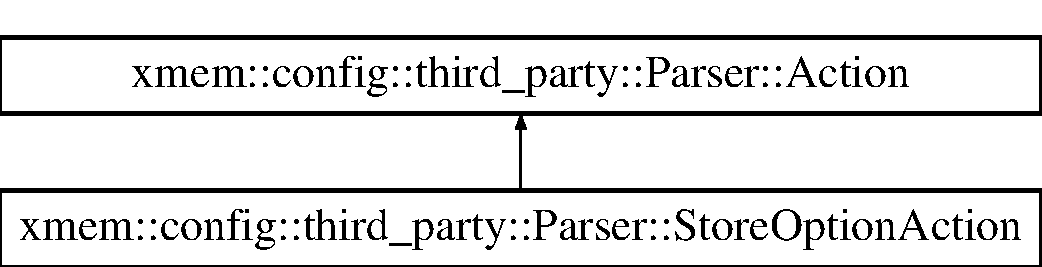
\includegraphics[height=2.000000cm]{classxmem_1_1config_1_1third__party_1_1_parser_1_1_store_option_action}
\end{center}
\end{figure}
\subsection*{Public Member Functions}
\begin{DoxyCompactItemize}
\item 
\hyperlink{classxmem_1_1config_1_1third__party_1_1_parser_1_1_store_option_action_aa6e4863f12c3f40b38d1571e75066aa4}{Store\+Option\+Action} (\hyperlink{classxmem_1_1config_1_1third__party_1_1_parser}{Parser} \&parser\+\_\+, \hyperlink{classxmem_1_1config_1_1third__party_1_1_option}{Option} options\+\_\+\mbox{[}$\,$\mbox{]}, \hyperlink{classxmem_1_1config_1_1third__party_1_1_option}{Option} buffer\+\_\+\mbox{[}$\,$\mbox{]}, int bufmax\+\_\+)
\begin{DoxyCompactList}\small\item\em Number of slots in {\ttfamily buffer}. {\ttfamily -\/1} means \char`\"{}large enough\char`\"{}. \end{DoxyCompactList}\item 
bool \hyperlink{classxmem_1_1config_1_1third__party_1_1_parser_1_1_store_option_action_ab34c68452366b58ad4163602cf5f435d}{perform} (\hyperlink{classxmem_1_1config_1_1third__party_1_1_option}{Option} \&option)
\begin{DoxyCompactList}\small\item\em Called by Parser\+::workhorse() for each \hyperlink{classxmem_1_1config_1_1third__party_1_1_option}{Option} that has been successfully parsed (including unknown options if they have a \hyperlink{structxmem_1_1config_1_1third__party_1_1_descriptor}{Descriptor} whose \hyperlink{structxmem_1_1config_1_1third__party_1_1_descriptor_a65b39f8d61de820bb5001d590e7dea5d}{Descriptor\+::check\+\_\+arg} does not return A\+R\+G\+\_\+\+I\+L\+L\+E\+G\+A\+L. \end{DoxyCompactList}\item 
bool \hyperlink{classxmem_1_1config_1_1third__party_1_1_parser_1_1_store_option_action_ad4e098cce0b0f97f025aec65d6226dff}{finished} (int numargs, const char $\ast$$\ast$args)
\begin{DoxyCompactList}\small\item\em Called by Parser\+::workhorse() after finishing the parse. \end{DoxyCompactList}\end{DoxyCompactItemize}


\subsection{Constructor \& Destructor Documentation}
\hypertarget{classxmem_1_1config_1_1third__party_1_1_parser_1_1_store_option_action_aa6e4863f12c3f40b38d1571e75066aa4}{}\index{xmem\+::config\+::third\+\_\+party\+::\+Parser\+::\+Store\+Option\+Action@{xmem\+::config\+::third\+\_\+party\+::\+Parser\+::\+Store\+Option\+Action}!Store\+Option\+Action@{Store\+Option\+Action}}
\index{Store\+Option\+Action@{Store\+Option\+Action}!xmem\+::config\+::third\+\_\+party\+::\+Parser\+::\+Store\+Option\+Action@{xmem\+::config\+::third\+\_\+party\+::\+Parser\+::\+Store\+Option\+Action}}
\subsubsection[{Store\+Option\+Action}]{\setlength{\rightskip}{0pt plus 5cm}xmem\+::config\+::third\+\_\+party\+::\+Parser\+::\+Store\+Option\+Action\+::\+Store\+Option\+Action (
\begin{DoxyParamCaption}
\item[{{\bf Parser} \&}]{parser\+\_\+, }
\item[{{\bf Option}}]{options\+\_\+\mbox{[}$\,$\mbox{]}, }
\item[{{\bf Option}}]{buffer\+\_\+\mbox{[}$\,$\mbox{]}, }
\item[{int}]{bufmax\+\_\+}
\end{DoxyParamCaption}
)\hspace{0.3cm}{\ttfamily [inline]}}\label{classxmem_1_1config_1_1third__party_1_1_parser_1_1_store_option_action_aa6e4863f12c3f40b38d1571e75066aa4}


Number of slots in {\ttfamily buffer}. {\ttfamily -\/1} means \char`\"{}large enough\char`\"{}. 

Creates a new Store\+Option action. 
\begin{DoxyParams}{Parameters}
{\em parser\+\_\+} & the parser whose op\+\_\+count should be updated. \\
\hline
{\em options\+\_\+} & each \hyperlink{classxmem_1_1config_1_1third__party_1_1_option}{Option} {\ttfamily o} is chained into the linked list {\ttfamily options\+\_\+}\mbox{[}o.\+desc-\/$>$index\mbox{]} \\
\hline
{\em buffer\+\_\+} & each \hyperlink{classxmem_1_1config_1_1third__party_1_1_option}{Option} is appended to this array as long as there\textquotesingle{}s a free slot. \\
\hline
{\em bufmax\+\_\+} & number of slots in {\ttfamily buffer\+\_\+}. {\ttfamily -\/1} means \char`\"{}large enough\char`\"{}. \\
\hline
\end{DoxyParams}


\subsection{Member Function Documentation}
\hypertarget{classxmem_1_1config_1_1third__party_1_1_parser_1_1_store_option_action_ad4e098cce0b0f97f025aec65d6226dff}{}\index{xmem\+::config\+::third\+\_\+party\+::\+Parser\+::\+Store\+Option\+Action@{xmem\+::config\+::third\+\_\+party\+::\+Parser\+::\+Store\+Option\+Action}!finished@{finished}}
\index{finished@{finished}!xmem\+::config\+::third\+\_\+party\+::\+Parser\+::\+Store\+Option\+Action@{xmem\+::config\+::third\+\_\+party\+::\+Parser\+::\+Store\+Option\+Action}}
\subsubsection[{finished}]{\setlength{\rightskip}{0pt plus 5cm}bool xmem\+::config\+::third\+\_\+party\+::\+Parser\+::\+Store\+Option\+Action\+::finished (
\begin{DoxyParamCaption}
\item[{int}]{numargs, }
\item[{const char $\ast$$\ast$}]{args}
\end{DoxyParamCaption}
)\hspace{0.3cm}{\ttfamily [inline]}, {\ttfamily [virtual]}}\label{classxmem_1_1config_1_1third__party_1_1_parser_1_1_store_option_action_ad4e098cce0b0f97f025aec65d6226dff}


Called by Parser\+::workhorse() after finishing the parse. 


\begin{DoxyParams}{Parameters}
{\em numargs} & the number of non-\/option arguments remaining \\
\hline
{\em args} & pointer to the first remaining non-\/option argument (if numargs $>$ 0).\\
\hline
\end{DoxyParams}
\begin{DoxyReturn}{Returns}
{\ttfamily false} iff a fatal error has occurred. 
\end{DoxyReturn}


Reimplemented from \hyperlink{structxmem_1_1config_1_1third__party_1_1_parser_1_1_action_a8f392f5dd42f483fa45ae5d83c9389ac}{xmem\+::config\+::third\+\_\+party\+::\+Parser\+::\+Action}.

\hypertarget{classxmem_1_1config_1_1third__party_1_1_parser_1_1_store_option_action_ab34c68452366b58ad4163602cf5f435d}{}\index{xmem\+::config\+::third\+\_\+party\+::\+Parser\+::\+Store\+Option\+Action@{xmem\+::config\+::third\+\_\+party\+::\+Parser\+::\+Store\+Option\+Action}!perform@{perform}}
\index{perform@{perform}!xmem\+::config\+::third\+\_\+party\+::\+Parser\+::\+Store\+Option\+Action@{xmem\+::config\+::third\+\_\+party\+::\+Parser\+::\+Store\+Option\+Action}}
\subsubsection[{perform}]{\setlength{\rightskip}{0pt plus 5cm}bool xmem\+::config\+::third\+\_\+party\+::\+Parser\+::\+Store\+Option\+Action\+::perform (
\begin{DoxyParamCaption}
\item[{{\bf Option} \&}]{}
\end{DoxyParamCaption}
)\hspace{0.3cm}{\ttfamily [inline]}, {\ttfamily [virtual]}}\label{classxmem_1_1config_1_1third__party_1_1_parser_1_1_store_option_action_ab34c68452366b58ad4163602cf5f435d}


Called by Parser\+::workhorse() for each \hyperlink{classxmem_1_1config_1_1third__party_1_1_option}{Option} that has been successfully parsed (including unknown options if they have a \hyperlink{structxmem_1_1config_1_1third__party_1_1_descriptor}{Descriptor} whose \hyperlink{structxmem_1_1config_1_1third__party_1_1_descriptor_a65b39f8d61de820bb5001d590e7dea5d}{Descriptor\+::check\+\_\+arg} does not return A\+R\+G\+\_\+\+I\+L\+L\+E\+G\+A\+L. 

Returns {\ttfamily false} iff a fatal error has occured and the parse should be aborted. 

Reimplemented from \hyperlink{structxmem_1_1config_1_1third__party_1_1_parser_1_1_action_aeffc43365955b3dc5f54552093518aa5}{xmem\+::config\+::third\+\_\+party\+::\+Parser\+::\+Action}.



The documentation for this class was generated from the following file\+:\begin{DoxyCompactItemize}
\item 
src/config/third\+\_\+party/\hyperlink{optionparser_8h}{optionparser.\+h}\end{DoxyCompactItemize}

\hypertarget{structxmem_1_1config_1_1third__party_1_1_print_usage_implementation_1_1_stream_writer}{}\section{xmem\+:\+:config\+:\+:third\+\_\+party\+:\+:Print\+Usage\+Implementation\+:\+:Stream\+Writer$<$ Function, Stream $>$ Struct Template Reference}
\label{structxmem_1_1config_1_1third__party_1_1_print_usage_implementation_1_1_stream_writer}\index{xmem\+::config\+::third\+\_\+party\+::\+Print\+Usage\+Implementation\+::\+Stream\+Writer$<$ Function, Stream $>$@{xmem\+::config\+::third\+\_\+party\+::\+Print\+Usage\+Implementation\+::\+Stream\+Writer$<$ Function, Stream $>$}}
Inheritance diagram for xmem\+:\+:config\+:\+:third\+\_\+party\+:\+:Print\+Usage\+Implementation\+:\+:Stream\+Writer$<$ Function, Stream $>$\+:\begin{figure}[H]
\begin{center}
\leavevmode
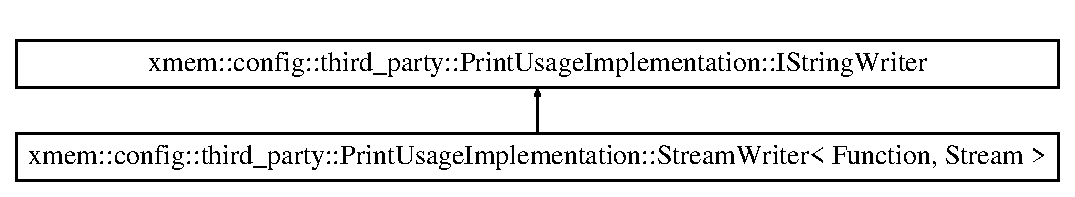
\includegraphics[height=2.000000cm]{structxmem_1_1config_1_1third__party_1_1_print_usage_implementation_1_1_stream_writer}
\end{center}
\end{figure}
\subsection*{Public Member Functions}
\begin{DoxyCompactItemize}
\item 
\hypertarget{structxmem_1_1config_1_1third__party_1_1_print_usage_implementation_1_1_stream_writer_aa5deaf2391cf05fc97ded29011eb345c}{}virtual void \hyperlink{structxmem_1_1config_1_1third__party_1_1_print_usage_implementation_1_1_stream_writer_aa5deaf2391cf05fc97ded29011eb345c}{operator()} (const char $\ast$str, int size)\label{structxmem_1_1config_1_1third__party_1_1_print_usage_implementation_1_1_stream_writer_aa5deaf2391cf05fc97ded29011eb345c}

\begin{DoxyCompactList}\small\item\em Writes the given number of chars beginning at the given pointer somewhere. \end{DoxyCompactList}\item 
\hypertarget{structxmem_1_1config_1_1third__party_1_1_print_usage_implementation_1_1_stream_writer_ab09e3fe226950f1d06c8e8e0b15ad32c}{}{\bfseries Stream\+Writer} (Function $\ast$w, Stream $\ast$s)\label{structxmem_1_1config_1_1third__party_1_1_print_usage_implementation_1_1_stream_writer_ab09e3fe226950f1d06c8e8e0b15ad32c}

\end{DoxyCompactItemize}
\subsection*{Public Attributes}
\begin{DoxyCompactItemize}
\item 
\hypertarget{structxmem_1_1config_1_1third__party_1_1_print_usage_implementation_1_1_stream_writer_acf48d2de031f76c609ab518fc757cfc1}{}Function $\ast$ {\bfseries fwrite}\label{structxmem_1_1config_1_1third__party_1_1_print_usage_implementation_1_1_stream_writer_acf48d2de031f76c609ab518fc757cfc1}

\item 
\hypertarget{structxmem_1_1config_1_1third__party_1_1_print_usage_implementation_1_1_stream_writer_ad0c294cda61db3cc2f7776def7466217}{}Stream $\ast$ {\bfseries stream}\label{structxmem_1_1config_1_1third__party_1_1_print_usage_implementation_1_1_stream_writer_ad0c294cda61db3cc2f7776def7466217}

\end{DoxyCompactItemize}


The documentation for this struct was generated from the following file\+:\begin{DoxyCompactItemize}
\item 
src/include/\hyperlink{optionparser_8h}{optionparser.\+h}\end{DoxyCompactItemize}

\hypertarget{structxmem_1_1config_1_1third__party_1_1_print_usage_implementation_1_1_syscall_writer}{\section{xmem\-:\-:config\-:\-:third\-\_\-party\-:\-:Print\-Usage\-Implementation\-:\-:Syscall\-Writer$<$ Syscall $>$ Struct Template Reference}
\label{structxmem_1_1config_1_1third__party_1_1_print_usage_implementation_1_1_syscall_writer}\index{xmem\-::config\-::third\-\_\-party\-::\-Print\-Usage\-Implementation\-::\-Syscall\-Writer$<$ Syscall $>$@{xmem\-::config\-::third\-\_\-party\-::\-Print\-Usage\-Implementation\-::\-Syscall\-Writer$<$ Syscall $>$}}
}
Inheritance diagram for xmem\-:\-:config\-:\-:third\-\_\-party\-:\-:Print\-Usage\-Implementation\-:\-:Syscall\-Writer$<$ Syscall $>$\-:\begin{figure}[H]
\begin{center}
\leavevmode
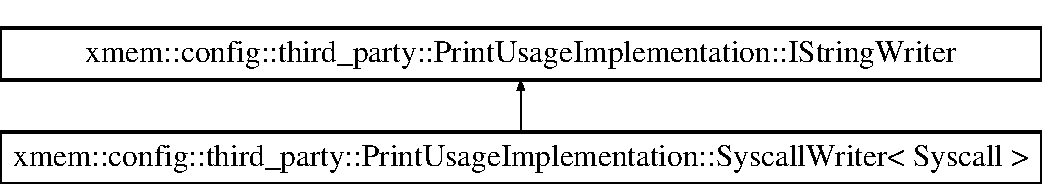
\includegraphics[height=2.000000cm]{structxmem_1_1config_1_1third__party_1_1_print_usage_implementation_1_1_syscall_writer}
\end{center}
\end{figure}
\subsection*{Public Member Functions}
\begin{DoxyCompactItemize}
\item 
\hypertarget{structxmem_1_1config_1_1third__party_1_1_print_usage_implementation_1_1_syscall_writer_abe35fdd4b67e221c5d6a3972a4970fb3}{virtual void \hyperlink{structxmem_1_1config_1_1third__party_1_1_print_usage_implementation_1_1_syscall_writer_abe35fdd4b67e221c5d6a3972a4970fb3}{operator()} (const char $\ast$str, int size)}\label{structxmem_1_1config_1_1third__party_1_1_print_usage_implementation_1_1_syscall_writer_abe35fdd4b67e221c5d6a3972a4970fb3}

\begin{DoxyCompactList}\small\item\em Writes the given number of chars beginning at the given pointer somewhere. \end{DoxyCompactList}\item 
\hypertarget{structxmem_1_1config_1_1third__party_1_1_print_usage_implementation_1_1_syscall_writer_a0787970dd79c70174d96b4ac9a05cacd}{{\bfseries Syscall\-Writer} (Syscall $\ast$w, int f)}\label{structxmem_1_1config_1_1third__party_1_1_print_usage_implementation_1_1_syscall_writer_a0787970dd79c70174d96b4ac9a05cacd}

\end{DoxyCompactItemize}
\subsection*{Public Attributes}
\begin{DoxyCompactItemize}
\item 
\hypertarget{structxmem_1_1config_1_1third__party_1_1_print_usage_implementation_1_1_syscall_writer_a437e8105a1e0b45e514246caed539664}{Syscall $\ast$ {\bfseries write}}\label{structxmem_1_1config_1_1third__party_1_1_print_usage_implementation_1_1_syscall_writer_a437e8105a1e0b45e514246caed539664}

\item 
\hypertarget{structxmem_1_1config_1_1third__party_1_1_print_usage_implementation_1_1_syscall_writer_a9652df23c84135075bb5468bb39a7064}{int {\bfseries fd}}\label{structxmem_1_1config_1_1third__party_1_1_print_usage_implementation_1_1_syscall_writer_a9652df23c84135075bb5468bb39a7064}

\end{DoxyCompactItemize}


The documentation for this struct was generated from the following file\-:\begin{DoxyCompactItemize}
\item 
src/include/\hyperlink{optionparser_8h}{optionparser.\-h}\end{DoxyCompactItemize}

\hypertarget{structxmem_1_1config_1_1third__party_1_1_print_usage_implementation_1_1_temporary_writer}{}\section{xmem\+:\+:config\+:\+:third\+\_\+party\+:\+:Print\+Usage\+Implementation\+:\+:Temporary\+Writer$<$ Temporary $>$ Struct Template Reference}
\label{structxmem_1_1config_1_1third__party_1_1_print_usage_implementation_1_1_temporary_writer}\index{xmem\+::config\+::third\+\_\+party\+::\+Print\+Usage\+Implementation\+::\+Temporary\+Writer$<$ Temporary $>$@{xmem\+::config\+::third\+\_\+party\+::\+Print\+Usage\+Implementation\+::\+Temporary\+Writer$<$ Temporary $>$}}
Inheritance diagram for xmem\+:\+:config\+:\+:third\+\_\+party\+:\+:Print\+Usage\+Implementation\+:\+:Temporary\+Writer$<$ Temporary $>$\+:\begin{figure}[H]
\begin{center}
\leavevmode
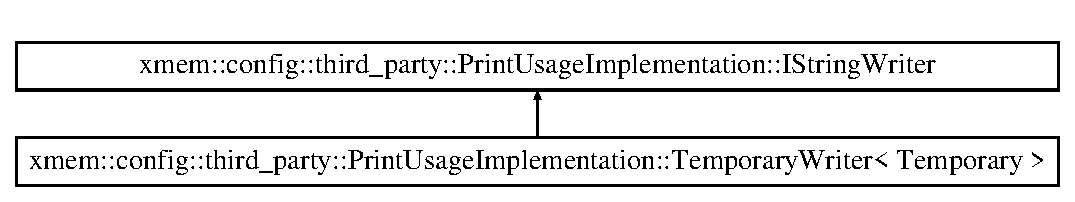
\includegraphics[height=2.000000cm]{structxmem_1_1config_1_1third__party_1_1_print_usage_implementation_1_1_temporary_writer}
\end{center}
\end{figure}
\subsection*{Public Member Functions}
\begin{DoxyCompactItemize}
\item 
\hypertarget{structxmem_1_1config_1_1third__party_1_1_print_usage_implementation_1_1_temporary_writer_a0498e8ecbdacb8d62612ed353baef8a4}{}virtual void \hyperlink{structxmem_1_1config_1_1third__party_1_1_print_usage_implementation_1_1_temporary_writer_a0498e8ecbdacb8d62612ed353baef8a4}{operator()} (const char $\ast$str, int size)\label{structxmem_1_1config_1_1third__party_1_1_print_usage_implementation_1_1_temporary_writer_a0498e8ecbdacb8d62612ed353baef8a4}

\begin{DoxyCompactList}\small\item\em Writes the given number of chars beginning at the given pointer somewhere. \end{DoxyCompactList}\item 
\hypertarget{structxmem_1_1config_1_1third__party_1_1_print_usage_implementation_1_1_temporary_writer_a72507591866203f8f9fce1d565f24859}{}{\bfseries Temporary\+Writer} (const Temporary \&u)\label{structxmem_1_1config_1_1third__party_1_1_print_usage_implementation_1_1_temporary_writer_a72507591866203f8f9fce1d565f24859}

\end{DoxyCompactItemize}
\subsection*{Public Attributes}
\begin{DoxyCompactItemize}
\item 
\hypertarget{structxmem_1_1config_1_1third__party_1_1_print_usage_implementation_1_1_temporary_writer_ad77042b28c27077df291dae5021a5065}{}const Temporary \& {\bfseries userstream}\label{structxmem_1_1config_1_1third__party_1_1_print_usage_implementation_1_1_temporary_writer_ad77042b28c27077df291dae5021a5065}

\end{DoxyCompactItemize}


The documentation for this struct was generated from the following file\+:\begin{DoxyCompactItemize}
\item 
src/include/\hyperlink{optionparser_8h}{optionparser.\+h}\end{DoxyCompactItemize}

\hypertarget{classxmem_1_1thread_1_1_thread}{}\section{xmem\+:\+:thread\+:\+:Thread Class Reference}
\label{classxmem_1_1thread_1_1_thread}\index{xmem\+::thread\+::\+Thread@{xmem\+::thread\+::\+Thread}}


a nice wrapped thread interface independent of particular O\+S A\+P\+I  




{\ttfamily \#include $<$Thread.\+h$>$}

\subsection*{Public Member Functions}
\begin{DoxyCompactItemize}
\item 
\hyperlink{classxmem_1_1thread_1_1_thread_a3248f8f92c293da9c20b78f443e61d76}{Thread} (\hyperlink{classxmem_1_1thread_1_1_runnable}{Runnable} $\ast$target)
\item 
\hyperlink{classxmem_1_1thread_1_1_thread_a37d9edd3a1a776cbc27dedff949c9726}{$\sim$\+Thread} ()
\item 
bool \hyperlink{classxmem_1_1thread_1_1_thread_a205afc741b86116bba9356b620a71cdf}{create} ()
\item 
bool \hyperlink{classxmem_1_1thread_1_1_thread_ac6142aac30e463bd99d703743f559d40}{start} ()
\item 
bool \hyperlink{classxmem_1_1thread_1_1_thread_a7550e894f4a83043fe4a4e93aee2def6}{create\+\_\+and\+\_\+start} ()
\item 
bool \hyperlink{classxmem_1_1thread_1_1_thread_ab1515cbc6982541f5327ff71a8d97a45}{join} (int32\+\_\+t timeout)
\item 
bool \hyperlink{classxmem_1_1thread_1_1_thread_a5d52b4357af2956e10fd72d80d540cf1}{cancel} ()
\item 
int32\+\_\+t \hyperlink{classxmem_1_1thread_1_1_thread_a6557774d3e8cf0bd92e8ba372cd23b85}{get\+Exit\+Code} ()
\item 
bool \hyperlink{classxmem_1_1thread_1_1_thread_a453a8b976b95c33d94b07fbca2ac414a}{started} ()
\item 
bool \hyperlink{classxmem_1_1thread_1_1_thread_a6d6ccbf6832d66803c6a527bad3943d8}{completed} ()
\item 
bool \hyperlink{classxmem_1_1thread_1_1_thread_ab91a2a9e8beb035106ba2d46ab32153c}{valid\+Target} ()
\item 
bool \hyperlink{classxmem_1_1thread_1_1_thread_a6a5f80bf0bca5ea5b18246aa2b1af250}{created} ()
\item 
bool \hyperlink{classxmem_1_1thread_1_1_thread_ab5c96a075727d5ffbec86213517a1795}{is\+Thread\+Suspended} ()
\item 
bool \hyperlink{classxmem_1_1thread_1_1_thread_afd810140b83b3a2ad90a425ea92dc366}{is\+Thread\+Running} ()
\item 
\hyperlink{classxmem_1_1thread_1_1_runnable}{Runnable} $\ast$ \hyperlink{classxmem_1_1thread_1_1_thread_a0cb4d94dd3f3d885794ce596a5198595}{get\+Target} ()
\end{DoxyCompactItemize}


\subsection{Detailed Description}
a nice wrapped thread interface independent of particular O\+S A\+P\+I 

\subsection{Constructor \& Destructor Documentation}
\hypertarget{classxmem_1_1thread_1_1_thread_a3248f8f92c293da9c20b78f443e61d76}{}\index{xmem\+::thread\+::\+Thread@{xmem\+::thread\+::\+Thread}!Thread@{Thread}}
\index{Thread@{Thread}!xmem\+::thread\+::\+Thread@{xmem\+::thread\+::\+Thread}}
\subsubsection[{Thread}]{\setlength{\rightskip}{0pt plus 5cm}Thread\+::\+Thread (
\begin{DoxyParamCaption}
\item[{{\bf Runnable} $\ast$}]{target}
\end{DoxyParamCaption}
)}\label{classxmem_1_1thread_1_1_thread_a3248f8f92c293da9c20b78f443e61d76}
Constructor. Does not actually create the real thread or run it. 
\begin{DoxyParams}{Parameters}
{\em target} & The target object to do some work with in a new thread. \\
\hline
\end{DoxyParams}
\hypertarget{classxmem_1_1thread_1_1_thread_a37d9edd3a1a776cbc27dedff949c9726}{}\index{xmem\+::thread\+::\+Thread@{xmem\+::thread\+::\+Thread}!````~Thread@{$\sim$\+Thread}}
\index{````~Thread@{$\sim$\+Thread}!xmem\+::thread\+::\+Thread@{xmem\+::thread\+::\+Thread}}
\subsubsection[{$\sim$\+Thread}]{\setlength{\rightskip}{0pt plus 5cm}Thread\+::$\sim$\+Thread (
\begin{DoxyParamCaption}
{}
\end{DoxyParamCaption}
)}\label{classxmem_1_1thread_1_1_thread_a37d9edd3a1a776cbc27dedff949c9726}
Destructor. Immediately cancels the thread if it exists. This can be unsafe! 

\subsection{Member Function Documentation}
\hypertarget{classxmem_1_1thread_1_1_thread_a5d52b4357af2956e10fd72d80d540cf1}{}\index{xmem\+::thread\+::\+Thread@{xmem\+::thread\+::\+Thread}!cancel@{cancel}}
\index{cancel@{cancel}!xmem\+::thread\+::\+Thread@{xmem\+::thread\+::\+Thread}}
\subsubsection[{cancel}]{\setlength{\rightskip}{0pt plus 5cm}bool Thread\+::cancel (
\begin{DoxyParamCaption}
{}
\end{DoxyParamCaption}
)}\label{classxmem_1_1thread_1_1_thread_a5d52b4357af2956e10fd72d80d540cf1}
Cancels the worker thread immediately. This should only be done in emergencies, as it is effectively killed and undefined behavior might occur. \begin{DoxyReturn}{Returns}
true if the worker thread was successfully killed. 
\end{DoxyReturn}
\hypertarget{classxmem_1_1thread_1_1_thread_a6d6ccbf6832d66803c6a527bad3943d8}{}\index{xmem\+::thread\+::\+Thread@{xmem\+::thread\+::\+Thread}!completed@{completed}}
\index{completed@{completed}!xmem\+::thread\+::\+Thread@{xmem\+::thread\+::\+Thread}}
\subsubsection[{completed}]{\setlength{\rightskip}{0pt plus 5cm}bool Thread\+::completed (
\begin{DoxyParamCaption}
{}
\end{DoxyParamCaption}
)}\label{classxmem_1_1thread_1_1_thread_a6d6ccbf6832d66803c6a527bad3943d8}
\begin{DoxyReturn}{Returns}
true if the thread completed, regardless of the manner in which it terminated. Returns false if it has not been started. 
\end{DoxyReturn}
\hypertarget{classxmem_1_1thread_1_1_thread_a205afc741b86116bba9356b620a71cdf}{}\index{xmem\+::thread\+::\+Thread@{xmem\+::thread\+::\+Thread}!create@{create}}
\index{create@{create}!xmem\+::thread\+::\+Thread@{xmem\+::thread\+::\+Thread}}
\subsubsection[{create}]{\setlength{\rightskip}{0pt plus 5cm}bool Thread\+::create (
\begin{DoxyParamCaption}
{}
\end{DoxyParamCaption}
)}\label{classxmem_1_1thread_1_1_thread_a205afc741b86116bba9356b620a71cdf}
Creates the thread if the target \hyperlink{classxmem_1_1thread_1_1_runnable}{Runnable} is valid, but does not start running it. \begin{DoxyReturn}{Returns}
true if the thread was successfully created. 
\end{DoxyReturn}
\hypertarget{classxmem_1_1thread_1_1_thread_a7550e894f4a83043fe4a4e93aee2def6}{}\index{xmem\+::thread\+::\+Thread@{xmem\+::thread\+::\+Thread}!create\+\_\+and\+\_\+start@{create\+\_\+and\+\_\+start}}
\index{create\+\_\+and\+\_\+start@{create\+\_\+and\+\_\+start}!xmem\+::thread\+::\+Thread@{xmem\+::thread\+::\+Thread}}
\subsubsection[{create\+\_\+and\+\_\+start}]{\setlength{\rightskip}{0pt plus 5cm}bool Thread\+::create\+\_\+and\+\_\+start (
\begin{DoxyParamCaption}
{}
\end{DoxyParamCaption}
)}\label{classxmem_1_1thread_1_1_thread_a7550e894f4a83043fe4a4e93aee2def6}
Creates and starts the thread immediately if the target \hyperlink{classxmem_1_1thread_1_1_runnable}{Runnable} is valid. This invokes the run() method in the \hyperlink{classxmem_1_1thread_1_1_runnable}{Runnable} target that was passed in the constructor. \begin{DoxyReturn}{Returns}
true if the thread was successfully created and started. 
\end{DoxyReturn}
\hypertarget{classxmem_1_1thread_1_1_thread_a6a5f80bf0bca5ea5b18246aa2b1af250}{}\index{xmem\+::thread\+::\+Thread@{xmem\+::thread\+::\+Thread}!created@{created}}
\index{created@{created}!xmem\+::thread\+::\+Thread@{xmem\+::thread\+::\+Thread}}
\subsubsection[{created}]{\setlength{\rightskip}{0pt plus 5cm}bool Thread\+::created (
\begin{DoxyParamCaption}
{}
\end{DoxyParamCaption}
)}\label{classxmem_1_1thread_1_1_thread_a6a5f80bf0bca5ea5b18246aa2b1af250}
\begin{DoxyReturn}{Returns}
true if the thread has been created successfully. 
\end{DoxyReturn}
\hypertarget{classxmem_1_1thread_1_1_thread_a6557774d3e8cf0bd92e8ba372cd23b85}{}\index{xmem\+::thread\+::\+Thread@{xmem\+::thread\+::\+Thread}!get\+Exit\+Code@{get\+Exit\+Code}}
\index{get\+Exit\+Code@{get\+Exit\+Code}!xmem\+::thread\+::\+Thread@{xmem\+::thread\+::\+Thread}}
\subsubsection[{get\+Exit\+Code}]{\setlength{\rightskip}{0pt plus 5cm}int32\+\_\+t Thread\+::get\+Exit\+Code (
\begin{DoxyParamCaption}
{}
\end{DoxyParamCaption}
)}\label{classxmem_1_1thread_1_1_thread_a6557774d3e8cf0bd92e8ba372cd23b85}
\begin{DoxyReturn}{Returns}
the exit code of the worker thread if it completed. If it did not complete or has not started, returns 0. 
\end{DoxyReturn}
\hypertarget{classxmem_1_1thread_1_1_thread_a0cb4d94dd3f3d885794ce596a5198595}{}\index{xmem\+::thread\+::\+Thread@{xmem\+::thread\+::\+Thread}!get\+Target@{get\+Target}}
\index{get\+Target@{get\+Target}!xmem\+::thread\+::\+Thread@{xmem\+::thread\+::\+Thread}}
\subsubsection[{get\+Target}]{\setlength{\rightskip}{0pt plus 5cm}{\bf Runnable} $\ast$ Thread\+::get\+Target (
\begin{DoxyParamCaption}
{}
\end{DoxyParamCaption}
)}\label{classxmem_1_1thread_1_1_thread_a0cb4d94dd3f3d885794ce596a5198595}
\begin{DoxyReturn}{Returns}
a pointer to the target \hyperlink{classxmem_1_1thread_1_1_runnable}{Runnable} object 
\end{DoxyReturn}
\hypertarget{classxmem_1_1thread_1_1_thread_afd810140b83b3a2ad90a425ea92dc366}{}\index{xmem\+::thread\+::\+Thread@{xmem\+::thread\+::\+Thread}!is\+Thread\+Running@{is\+Thread\+Running}}
\index{is\+Thread\+Running@{is\+Thread\+Running}!xmem\+::thread\+::\+Thread@{xmem\+::thread\+::\+Thread}}
\subsubsection[{is\+Thread\+Running}]{\setlength{\rightskip}{0pt plus 5cm}bool Thread\+::is\+Thread\+Running (
\begin{DoxyParamCaption}
{}
\end{DoxyParamCaption}
)}\label{classxmem_1_1thread_1_1_thread_afd810140b83b3a2ad90a425ea92dc366}
\begin{DoxyReturn}{Returns}
true if the thread is running. Returns false if the thread has not been created. 
\end{DoxyReturn}
\hypertarget{classxmem_1_1thread_1_1_thread_ab5c96a075727d5ffbec86213517a1795}{}\index{xmem\+::thread\+::\+Thread@{xmem\+::thread\+::\+Thread}!is\+Thread\+Suspended@{is\+Thread\+Suspended}}
\index{is\+Thread\+Suspended@{is\+Thread\+Suspended}!xmem\+::thread\+::\+Thread@{xmem\+::thread\+::\+Thread}}
\subsubsection[{is\+Thread\+Suspended}]{\setlength{\rightskip}{0pt plus 5cm}bool Thread\+::is\+Thread\+Suspended (
\begin{DoxyParamCaption}
{}
\end{DoxyParamCaption}
)}\label{classxmem_1_1thread_1_1_thread_ab5c96a075727d5ffbec86213517a1795}
\begin{DoxyReturn}{Returns}
true if the thread is suspended. Returns false if the thread has not been created. 
\end{DoxyReturn}
\hypertarget{classxmem_1_1thread_1_1_thread_ab1515cbc6982541f5327ff71a8d97a45}{}\index{xmem\+::thread\+::\+Thread@{xmem\+::thread\+::\+Thread}!join@{join}}
\index{join@{join}!xmem\+::thread\+::\+Thread@{xmem\+::thread\+::\+Thread}}
\subsubsection[{join}]{\setlength{\rightskip}{0pt plus 5cm}bool Thread\+::join (
\begin{DoxyParamCaption}
\item[{int32\+\_\+t}]{timeout}
\end{DoxyParamCaption}
)}\label{classxmem_1_1thread_1_1_thread_ab1515cbc6982541f5327ff71a8d97a45}
Blocks the calling thread until the worker thread managed by this object terminates. If the worker thread has already terminated, returns immediately. If the worker has not yet started, returns immediately. 
\begin{DoxyParams}{Parameters}
{\em timeout} & timeout in milliseconds to wait for the thread. If 0, does not wait at all. If negative, waits indefinitely. \\
\hline
\end{DoxyParams}
\begin{DoxyReturn}{Returns}
true if the worker thread terminated successfully, false otherwise or if \hyperlink{classxmem_1_1thread_1_1_thread_ab1515cbc6982541f5327ff71a8d97a45}{join()} was not called legally. 
\end{DoxyReturn}
\hypertarget{classxmem_1_1thread_1_1_thread_ac6142aac30e463bd99d703743f559d40}{}\index{xmem\+::thread\+::\+Thread@{xmem\+::thread\+::\+Thread}!start@{start}}
\index{start@{start}!xmem\+::thread\+::\+Thread@{xmem\+::thread\+::\+Thread}}
\subsubsection[{start}]{\setlength{\rightskip}{0pt plus 5cm}bool Thread\+::start (
\begin{DoxyParamCaption}
{}
\end{DoxyParamCaption}
)}\label{classxmem_1_1thread_1_1_thread_ac6142aac30e463bd99d703743f559d40}
Starts the thread immediately if the thread has been created. This invokes the run() method in the \hyperlink{classxmem_1_1thread_1_1_runnable}{Runnable} target that was passed in the constructor. \begin{DoxyReturn}{Returns}
true if the thread was successfully started. 
\end{DoxyReturn}
\hypertarget{classxmem_1_1thread_1_1_thread_a453a8b976b95c33d94b07fbca2ac414a}{}\index{xmem\+::thread\+::\+Thread@{xmem\+::thread\+::\+Thread}!started@{started}}
\index{started@{started}!xmem\+::thread\+::\+Thread@{xmem\+::thread\+::\+Thread}}
\subsubsection[{started}]{\setlength{\rightskip}{0pt plus 5cm}bool Thread\+::started (
\begin{DoxyParamCaption}
{}
\end{DoxyParamCaption}
)}\label{classxmem_1_1thread_1_1_thread_a453a8b976b95c33d94b07fbca2ac414a}
\begin{DoxyReturn}{Returns}
true if the thread has been started, regardless if has completed or not. 
\end{DoxyReturn}
\hypertarget{classxmem_1_1thread_1_1_thread_ab91a2a9e8beb035106ba2d46ab32153c}{}\index{xmem\+::thread\+::\+Thread@{xmem\+::thread\+::\+Thread}!valid\+Target@{valid\+Target}}
\index{valid\+Target@{valid\+Target}!xmem\+::thread\+::\+Thread@{xmem\+::thread\+::\+Thread}}
\subsubsection[{valid\+Target}]{\setlength{\rightskip}{0pt plus 5cm}bool Thread\+::valid\+Target (
\begin{DoxyParamCaption}
{}
\end{DoxyParamCaption}
)}\label{classxmem_1_1thread_1_1_thread_ab91a2a9e8beb035106ba2d46ab32153c}
\begin{DoxyReturn}{Returns}
true if the \hyperlink{classxmem_1_1thread_1_1_runnable}{Runnable} target is valid. 
\end{DoxyReturn}


The documentation for this class was generated from the following files\+:\begin{DoxyCompactItemize}
\item 
src/include/\hyperlink{_thread_8h}{Thread.\+h}\item 
src/\hyperlink{_thread_8cpp}{Thread.\+cpp}\end{DoxyCompactItemize}

\hypertarget{classxmem_1_1benchmark_1_1_throughput_benchmark}{}\section{xmem\+:\+:benchmark\+:\+:Throughput\+Benchmark Class Reference}
\label{classxmem_1_1benchmark_1_1_throughput_benchmark}\index{xmem\+::benchmark\+::\+Throughput\+Benchmark@{xmem\+::benchmark\+::\+Throughput\+Benchmark}}


A type of benchmark that measures memory throughput either via sequential, strided sequential, or random access patterns.  




{\ttfamily \#include $<$Throughput\+Benchmark.\+h$>$}

Inheritance diagram for xmem\+:\+:benchmark\+:\+:Throughput\+Benchmark\+:\begin{figure}[H]
\begin{center}
\leavevmode
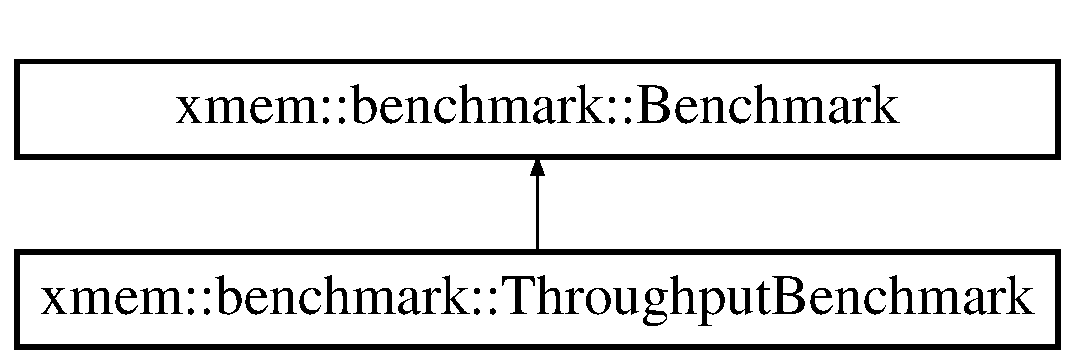
\includegraphics[height=2.000000cm]{classxmem_1_1benchmark_1_1_throughput_benchmark}
\end{center}
\end{figure}
\subsection*{Public Types}
\begin{DoxyCompactItemize}
\item 
\hypertarget{classxmem_1_1benchmark_1_1_throughput_benchmark_a21095b46866ebe68c75c3be14471a7b5}{}typedef int32\+\_\+t($\ast$ {\bfseries Throughput\+Bench\+Function}) (void $\ast$, void $\ast$)\label{classxmem_1_1benchmark_1_1_throughput_benchmark_a21095b46866ebe68c75c3be14471a7b5}

\end{DoxyCompactItemize}
\subsection*{Public Member Functions}
\begin{DoxyCompactItemize}
\item 
\hyperlink{classxmem_1_1benchmark_1_1_throughput_benchmark_a7f6fcc030500ebd3aed37d7eacea68dc}{Throughput\+Benchmark} (void $\ast$mem\+\_\+array, size\+\_\+t len, uint32\+\_\+t iterations, xmem\+::common\+::chunk\+\_\+size\+\_\+t chunk\+\_\+size, uint32\+\_\+t cpu\+\_\+node, uint32\+\_\+t mem\+\_\+node, uint32\+\_\+t num\+\_\+worker\+\_\+threads, std\+::string name, \hyperlink{classxmem_1_1timers_1_1_timer}{xmem\+::timers\+::\+Timer} $\ast$timer, std\+::vector$<$ \hyperlink{classxmem_1_1power_1_1_power_reader}{xmem\+::power\+::\+Power\+Reader} $\ast$ $>$ dram\+\_\+power\+\_\+readers, int64\+\_\+t stride\+\_\+size, xmem\+::common\+::pattern\+\_\+mode\+\_\+t pattern\+\_\+mode, xmem\+::common\+::rw\+\_\+mode\+\_\+t rw\+\_\+mode)
\begin{DoxyCompactList}\small\item\em Constructor. \end{DoxyCompactList}\item 
\hypertarget{classxmem_1_1benchmark_1_1_throughput_benchmark_ad4adc2b57b501862bfa415c4adfdef7e}{}virtual \hyperlink{classxmem_1_1benchmark_1_1_throughput_benchmark_ad4adc2b57b501862bfa415c4adfdef7e}{$\sim$\+Throughput\+Benchmark} ()\label{classxmem_1_1benchmark_1_1_throughput_benchmark_ad4adc2b57b501862bfa415c4adfdef7e}

\begin{DoxyCompactList}\small\item\em Destructor. \end{DoxyCompactList}\item 
virtual bool \hyperlink{classxmem_1_1benchmark_1_1_throughput_benchmark_a9f113e51d980830582148eb05c8810a3}{run} ()
\begin{DoxyCompactList}\small\item\em Runs the benchmark. \end{DoxyCompactList}\item 
\hypertarget{classxmem_1_1benchmark_1_1_throughput_benchmark_aab821d4beb68616c5a939bc2e493426e}{}virtual void \hyperlink{classxmem_1_1benchmark_1_1_throughput_benchmark_aab821d4beb68616c5a939bc2e493426e}{report\+\_\+benchmark\+\_\+info} ()\label{classxmem_1_1benchmark_1_1_throughput_benchmark_aab821d4beb68616c5a939bc2e493426e}

\begin{DoxyCompactList}\small\item\em Reports benchmark configuration details to the console. \end{DoxyCompactList}\item 
\hypertarget{classxmem_1_1benchmark_1_1_throughput_benchmark_a7df909bd544d1399e756a98bfbce2561}{}virtual void \hyperlink{classxmem_1_1benchmark_1_1_throughput_benchmark_a7df909bd544d1399e756a98bfbce2561}{report\+\_\+results} ()\label{classxmem_1_1benchmark_1_1_throughput_benchmark_a7df909bd544d1399e756a98bfbce2561}

\begin{DoxyCompactList}\small\item\em Reports results to the console. \end{DoxyCompactList}\item 
int64\+\_\+t \hyperlink{classxmem_1_1benchmark_1_1_throughput_benchmark_ad31b0fecafb174be0509581cda099d55}{get\+Stride\+Size} ()
\begin{DoxyCompactList}\small\item\em Gets the stride size for this benchmark. \end{DoxyCompactList}\item 
xmem\+::common\+::pattern\+\_\+mode\+\_\+t \hyperlink{classxmem_1_1benchmark_1_1_throughput_benchmark_a2c7dc699b2ae013edd9de871778dff7b}{get\+Pattern\+Mode} ()
\begin{DoxyCompactList}\small\item\em Gets the pattern mode for this benchmark. \end{DoxyCompactList}\item 
xmem\+::common\+::rw\+\_\+mode\+\_\+t \hyperlink{classxmem_1_1benchmark_1_1_throughput_benchmark_acd839b1c7a1d51ff3ce7921a36d65e98}{get\+R\+W\+Mode} ()
\begin{DoxyCompactList}\small\item\em Gets the read/write mode for this benchmark. \end{DoxyCompactList}\end{DoxyCompactItemize}
\subsection*{Additional Inherited Members}


\subsection{Detailed Description}
A type of benchmark that measures memory throughput either via sequential, strided sequential, or random access patterns. 

\subsection{Constructor \& Destructor Documentation}
\hypertarget{classxmem_1_1benchmark_1_1_throughput_benchmark_a7f6fcc030500ebd3aed37d7eacea68dc}{}\index{xmem\+::benchmark\+::\+Throughput\+Benchmark@{xmem\+::benchmark\+::\+Throughput\+Benchmark}!Throughput\+Benchmark@{Throughput\+Benchmark}}
\index{Throughput\+Benchmark@{Throughput\+Benchmark}!xmem\+::benchmark\+::\+Throughput\+Benchmark@{xmem\+::benchmark\+::\+Throughput\+Benchmark}}
\subsubsection[{Throughput\+Benchmark}]{\setlength{\rightskip}{0pt plus 5cm}Throughput\+Benchmark\+::\+Throughput\+Benchmark (
\begin{DoxyParamCaption}
\item[{void $\ast$}]{mem\+\_\+array, }
\item[{size\+\_\+t}]{len, }
\item[{uint32\+\_\+t}]{iterations, }
\item[{xmem\+::common\+::chunk\+\_\+size\+\_\+t}]{chunk\+\_\+size, }
\item[{uint32\+\_\+t}]{cpu\+\_\+node, }
\item[{uint32\+\_\+t}]{mem\+\_\+node, }
\item[{uint32\+\_\+t}]{num\+\_\+worker\+\_\+threads, }
\item[{std\+::string}]{name, }
\item[{{\bf xmem\+::timers\+::\+Timer} $\ast$}]{timer, }
\item[{std\+::vector$<$ {\bf xmem\+::power\+::\+Power\+Reader} $\ast$ $>$}]{dram\+\_\+power\+\_\+readers, }
\item[{int64\+\_\+t}]{stride\+\_\+size, }
\item[{xmem\+::common\+::pattern\+\_\+mode\+\_\+t}]{pattern\+\_\+mode, }
\item[{xmem\+::common\+::rw\+\_\+mode\+\_\+t}]{rw\+\_\+mode}
\end{DoxyParamCaption}
)}\label{classxmem_1_1benchmark_1_1_throughput_benchmark_a7f6fcc030500ebd3aed37d7eacea68dc}


Constructor. 


\begin{DoxyParams}{Parameters}
{\em mem\+\_\+array} & a pointer to a contiguous chunk of memory that has been allocated for benchmarking among the worker threads. This should be aligned to a 256-\/bit boundary and should be the working set size times number of threads large. \\
\hline
{\em len} & Length of the raw\+\_\+mem\+\_\+array in bytes. This should be a multiple of 4 K\+B pages. \\
\hline
{\em iterations} & Number of iterations (passes) to do of the complete benchmark. \\
\hline
{\em chunk\+\_\+size} & encoded size of an individual memory access. \\
\hline
{\em cpu\+\_\+node} & the logical C\+P\+U N\+U\+M\+A node to use in the benchmark \\
\hline
{\em mem\+\_\+node} & the logical memory N\+U\+M\+A node used in the benchmark \\
\hline
{\em num\+\_\+worker\+\_\+threads} & number of worker threads to use in the benchmark \\
\hline
{\em name} & name of the benchmark to use when reporting \\
\hline
{\em timer} & pointer to an existing Timer object \\
\hline
{\em dram\+\_\+power\+\_\+readers} & vector of pointers to Power\+Reader objects for measuring D\+R\+A\+M power \\
\hline
{\em stride\+\_\+size} & For sequential access patterns, the stride counted in chunks. Negative values mean reverse access pattern. A stride of 1 is purely sequential. \\
\hline
{\em pattern\+\_\+mode} & Indicates sequential or random access. \\
\hline
{\em rw\+\_\+mode} & Indicates reads or writes. T\+O\+D\+O\+: allow for a mixture \\
\hline
\end{DoxyParams}


\subsection{Member Function Documentation}
\hypertarget{classxmem_1_1benchmark_1_1_throughput_benchmark_a2c7dc699b2ae013edd9de871778dff7b}{}\index{xmem\+::benchmark\+::\+Throughput\+Benchmark@{xmem\+::benchmark\+::\+Throughput\+Benchmark}!get\+Pattern\+Mode@{get\+Pattern\+Mode}}
\index{get\+Pattern\+Mode@{get\+Pattern\+Mode}!xmem\+::benchmark\+::\+Throughput\+Benchmark@{xmem\+::benchmark\+::\+Throughput\+Benchmark}}
\subsubsection[{get\+Pattern\+Mode}]{\setlength{\rightskip}{0pt plus 5cm}pattern\+\_\+mode\+\_\+t Throughput\+Benchmark\+::get\+Pattern\+Mode (
\begin{DoxyParamCaption}
{}
\end{DoxyParamCaption}
)}\label{classxmem_1_1benchmark_1_1_throughput_benchmark_a2c7dc699b2ae013edd9de871778dff7b}


Gets the pattern mode for this benchmark. 

\begin{DoxyReturn}{Returns}
The pattern mode enumerator. 
\end{DoxyReturn}
\hypertarget{classxmem_1_1benchmark_1_1_throughput_benchmark_acd839b1c7a1d51ff3ce7921a36d65e98}{}\index{xmem\+::benchmark\+::\+Throughput\+Benchmark@{xmem\+::benchmark\+::\+Throughput\+Benchmark}!get\+R\+W\+Mode@{get\+R\+W\+Mode}}
\index{get\+R\+W\+Mode@{get\+R\+W\+Mode}!xmem\+::benchmark\+::\+Throughput\+Benchmark@{xmem\+::benchmark\+::\+Throughput\+Benchmark}}
\subsubsection[{get\+R\+W\+Mode}]{\setlength{\rightskip}{0pt plus 5cm}rw\+\_\+mode\+\_\+t Throughput\+Benchmark\+::get\+R\+W\+Mode (
\begin{DoxyParamCaption}
{}
\end{DoxyParamCaption}
)}\label{classxmem_1_1benchmark_1_1_throughput_benchmark_acd839b1c7a1d51ff3ce7921a36d65e98}


Gets the read/write mode for this benchmark. 

\begin{DoxyReturn}{Returns}
The read/write mix mode. 
\end{DoxyReturn}
\hypertarget{classxmem_1_1benchmark_1_1_throughput_benchmark_ad31b0fecafb174be0509581cda099d55}{}\index{xmem\+::benchmark\+::\+Throughput\+Benchmark@{xmem\+::benchmark\+::\+Throughput\+Benchmark}!get\+Stride\+Size@{get\+Stride\+Size}}
\index{get\+Stride\+Size@{get\+Stride\+Size}!xmem\+::benchmark\+::\+Throughput\+Benchmark@{xmem\+::benchmark\+::\+Throughput\+Benchmark}}
\subsubsection[{get\+Stride\+Size}]{\setlength{\rightskip}{0pt plus 5cm}int64\+\_\+t Throughput\+Benchmark\+::get\+Stride\+Size (
\begin{DoxyParamCaption}
{}
\end{DoxyParamCaption}
)}\label{classxmem_1_1benchmark_1_1_throughput_benchmark_ad31b0fecafb174be0509581cda099d55}


Gets the stride size for this benchmark. 

\begin{DoxyReturn}{Returns}
The stride size in chunks. 
\end{DoxyReturn}
\hypertarget{classxmem_1_1benchmark_1_1_throughput_benchmark_a9f113e51d980830582148eb05c8810a3}{}\index{xmem\+::benchmark\+::\+Throughput\+Benchmark@{xmem\+::benchmark\+::\+Throughput\+Benchmark}!run@{run}}
\index{run@{run}!xmem\+::benchmark\+::\+Throughput\+Benchmark@{xmem\+::benchmark\+::\+Throughput\+Benchmark}}
\subsubsection[{run}]{\setlength{\rightskip}{0pt plus 5cm}bool Throughput\+Benchmark\+::run (
\begin{DoxyParamCaption}
{}
\end{DoxyParamCaption}
)\hspace{0.3cm}{\ttfamily [virtual]}}\label{classxmem_1_1benchmark_1_1_throughput_benchmark_a9f113e51d980830582148eb05c8810a3}


Runs the benchmark. 

\begin{DoxyReturn}{Returns}
true on success 
\end{DoxyReturn}


Implements \hyperlink{classxmem_1_1benchmark_1_1_benchmark_aa0dbe60e525457770c835c6c72a0be6a}{xmem\+::benchmark\+::\+Benchmark}.



The documentation for this class was generated from the following files\+:\begin{DoxyCompactItemize}
\item 
src/include/\hyperlink{_throughput_benchmark_8h}{Throughput\+Benchmark.\+h}\item 
src/\hyperlink{_throughput_benchmark_8cpp}{Throughput\+Benchmark.\+cpp}\end{DoxyCompactItemize}

\hypertarget{classxmem_1_1benchmark_1_1_throughput_benchmark_worker}{}\section{xmem\+:\+:benchmark\+:\+:Throughput\+Benchmark\+Worker Class Reference}
\label{classxmem_1_1benchmark_1_1_throughput_benchmark_worker}\index{xmem\+::benchmark\+::\+Throughput\+Benchmark\+Worker@{xmem\+::benchmark\+::\+Throughput\+Benchmark\+Worker}}


Helper multithreading-\/friendly class to do the core throughput benchmark.  




{\ttfamily \#include $<$Throughput\+Benchmark\+Worker.\+h$>$}

Inheritance diagram for xmem\+:\+:benchmark\+:\+:Throughput\+Benchmark\+Worker\+:\begin{figure}[H]
\begin{center}
\leavevmode
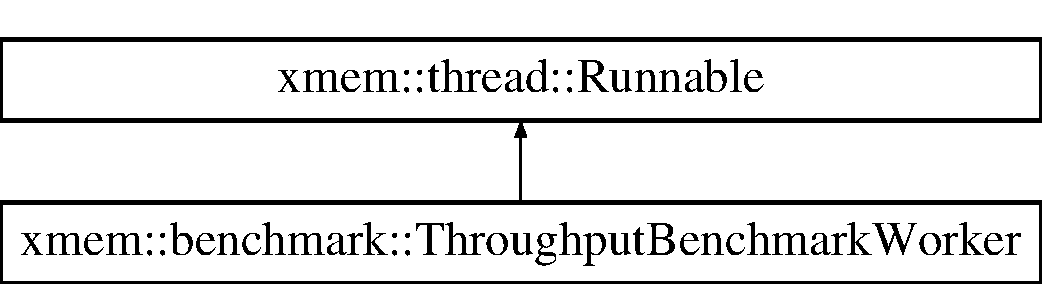
\includegraphics[height=2.000000cm]{classxmem_1_1benchmark_1_1_throughput_benchmark_worker}
\end{center}
\end{figure}
\subsection*{Public Types}
\begin{DoxyCompactItemize}
\item 
\hypertarget{classxmem_1_1benchmark_1_1_throughput_benchmark_worker_a4604cb1fd7108eb9d56007bfb3c6e54f}{}typedef int32\+\_\+t($\ast$ {\bfseries Bench\+Function}) (void $\ast$, void $\ast$)\label{classxmem_1_1benchmark_1_1_throughput_benchmark_worker_a4604cb1fd7108eb9d56007bfb3c6e54f}

\end{DoxyCompactItemize}
\subsection*{Public Member Functions}
\begin{DoxyCompactItemize}
\item 
\hyperlink{classxmem_1_1benchmark_1_1_throughput_benchmark_worker_a271c77940bc7cb45fcc395d3ed14361c}{Throughput\+Benchmark\+Worker} (void $\ast$mem\+\_\+array, size\+\_\+t len, Bench\+Function bench\+\_\+fptr, Bench\+Function dummy\+\_\+fptr, uint32\+\_\+t cpu\+\_\+affinity)
\begin{DoxyCompactList}\small\item\em Constructor. \end{DoxyCompactList}\item 
\hypertarget{classxmem_1_1benchmark_1_1_throughput_benchmark_worker_a021aae8513f5da78e04ba711e308b705}{}\hyperlink{classxmem_1_1benchmark_1_1_throughput_benchmark_worker_a021aae8513f5da78e04ba711e308b705}{$\sim$\+Throughput\+Benchmark\+Worker} ()\label{classxmem_1_1benchmark_1_1_throughput_benchmark_worker_a021aae8513f5da78e04ba711e308b705}

\begin{DoxyCompactList}\small\item\em Destructor. \end{DoxyCompactList}\item 
\hypertarget{classxmem_1_1benchmark_1_1_throughput_benchmark_worker_afb71dd763f55504ddabcabb24e0d6834}{}virtual void \hyperlink{classxmem_1_1benchmark_1_1_throughput_benchmark_worker_afb71dd763f55504ddabcabb24e0d6834}{run} ()\label{classxmem_1_1benchmark_1_1_throughput_benchmark_worker_afb71dd763f55504ddabcabb24e0d6834}

\begin{DoxyCompactList}\small\item\em Thread-\/safe worker method. \end{DoxyCompactList}\item 
size\+\_\+t \hyperlink{classxmem_1_1benchmark_1_1_throughput_benchmark_worker_a65dfa53d591ebf85ee3d1dfdd7c98f20}{get\+Len} ()
\begin{DoxyCompactList}\small\item\em Gets the length of the memory region used by this worker. \end{DoxyCompactList}\item 
uint64\+\_\+t \hyperlink{classxmem_1_1benchmark_1_1_throughput_benchmark_worker_aa3c3f95c0dd92e82391135cc57e1ab1f}{get\+Bytes\+Per\+Pass} ()
\begin{DoxyCompactList}\small\item\em Gets the number of bytes used in each pass of the benchmark by this worker. \end{DoxyCompactList}\item 
uint64\+\_\+t \hyperlink{classxmem_1_1benchmark_1_1_throughput_benchmark_worker_afc7a394e6a04e4fe72d82db3ca47cd62}{get\+Passes} ()
\begin{DoxyCompactList}\small\item\em Gets the number of passes for this worker. \end{DoxyCompactList}\item 
uint64\+\_\+t \hyperlink{classxmem_1_1benchmark_1_1_throughput_benchmark_worker_acf9ec8195f85292cc744b89b3ab0e6cc}{get\+Elapsed\+Ticks} ()
\begin{DoxyCompactList}\small\item\em Gets the elapsed ticks for this worker on the core benchmark kernel. \end{DoxyCompactList}\item 
uint64\+\_\+t \hyperlink{classxmem_1_1benchmark_1_1_throughput_benchmark_worker_a301d7c1f0f7400a9f4a8a4be66969319}{get\+Elapsed\+Dummy\+Ticks} ()
\begin{DoxyCompactList}\small\item\em Gets the elapsed ticks for this worker on the dummy version of the core benchmark kernel. \end{DoxyCompactList}\item 
uint64\+\_\+t \hyperlink{classxmem_1_1benchmark_1_1_throughput_benchmark_worker_aac1a7f68313e877f4f73d212d00d5289}{get\+Adjusted\+Ticks} ()
\begin{DoxyCompactList}\small\item\em Gets the adjusted ticks for this worker. This is elapsed ticks minus elapsed dummy ticks. \end{DoxyCompactList}\item 
bool \hyperlink{classxmem_1_1benchmark_1_1_throughput_benchmark_worker_af44781eee1ae525ce94ec83da6e7595e}{had\+Warning} ()
\begin{DoxyCompactList}\small\item\em Indicates whether worker\textquotesingle{}s results may be questionable/inaccurate/invalid. \end{DoxyCompactList}\end{DoxyCompactItemize}
\subsection*{Additional Inherited Members}


\subsection{Detailed Description}
Helper multithreading-\/friendly class to do the core throughput benchmark. 

\subsection{Constructor \& Destructor Documentation}
\hypertarget{classxmem_1_1benchmark_1_1_throughput_benchmark_worker_a271c77940bc7cb45fcc395d3ed14361c}{}\index{xmem\+::benchmark\+::\+Throughput\+Benchmark\+Worker@{xmem\+::benchmark\+::\+Throughput\+Benchmark\+Worker}!Throughput\+Benchmark\+Worker@{Throughput\+Benchmark\+Worker}}
\index{Throughput\+Benchmark\+Worker@{Throughput\+Benchmark\+Worker}!xmem\+::benchmark\+::\+Throughput\+Benchmark\+Worker@{xmem\+::benchmark\+::\+Throughput\+Benchmark\+Worker}}
\subsubsection[{Throughput\+Benchmark\+Worker}]{\setlength{\rightskip}{0pt plus 5cm}Throughput\+Benchmark\+Worker\+::\+Throughput\+Benchmark\+Worker (
\begin{DoxyParamCaption}
\item[{void $\ast$}]{mem\+\_\+array, }
\item[{size\+\_\+t}]{len, }
\item[{Bench\+Function}]{bench\+\_\+fptr, }
\item[{Bench\+Function}]{dummy\+\_\+fptr, }
\item[{uint32\+\_\+t}]{cpu\+\_\+affinity}
\end{DoxyParamCaption}
)}\label{classxmem_1_1benchmark_1_1_throughput_benchmark_worker_a271c77940bc7cb45fcc395d3ed14361c}


Constructor. 


\begin{DoxyParams}{Parameters}
{\em mem\+\_\+array} & Pointer to the memory region to use by this worker. \\
\hline
{\em len} & Length of the memory region to use by this worker. \\
\hline
{\em bench\+\_\+fptr} & Pointer to the core benchmark kernel to use. \\
\hline
{\em dummy\+\_\+fptr} & Pointer to the dummy version of the core benchmark kernel to use. \\
\hline
{\em cpu\+\_\+affinity} & Logical C\+P\+U identifier to lock this worker\textquotesingle{}s thread to. \\
\hline
\end{DoxyParams}


\subsection{Member Function Documentation}
\hypertarget{classxmem_1_1benchmark_1_1_throughput_benchmark_worker_aac1a7f68313e877f4f73d212d00d5289}{}\index{xmem\+::benchmark\+::\+Throughput\+Benchmark\+Worker@{xmem\+::benchmark\+::\+Throughput\+Benchmark\+Worker}!get\+Adjusted\+Ticks@{get\+Adjusted\+Ticks}}
\index{get\+Adjusted\+Ticks@{get\+Adjusted\+Ticks}!xmem\+::benchmark\+::\+Throughput\+Benchmark\+Worker@{xmem\+::benchmark\+::\+Throughput\+Benchmark\+Worker}}
\subsubsection[{get\+Adjusted\+Ticks}]{\setlength{\rightskip}{0pt plus 5cm}uint64\+\_\+t Throughput\+Benchmark\+Worker\+::get\+Adjusted\+Ticks (
\begin{DoxyParamCaption}
{}
\end{DoxyParamCaption}
)}\label{classxmem_1_1benchmark_1_1_throughput_benchmark_worker_aac1a7f68313e877f4f73d212d00d5289}


Gets the adjusted ticks for this worker. This is elapsed ticks minus elapsed dummy ticks. 

\begin{DoxyReturn}{Returns}
The adjusted ticks for this worker. 
\end{DoxyReturn}
\hypertarget{classxmem_1_1benchmark_1_1_throughput_benchmark_worker_aa3c3f95c0dd92e82391135cc57e1ab1f}{}\index{xmem\+::benchmark\+::\+Throughput\+Benchmark\+Worker@{xmem\+::benchmark\+::\+Throughput\+Benchmark\+Worker}!get\+Bytes\+Per\+Pass@{get\+Bytes\+Per\+Pass}}
\index{get\+Bytes\+Per\+Pass@{get\+Bytes\+Per\+Pass}!xmem\+::benchmark\+::\+Throughput\+Benchmark\+Worker@{xmem\+::benchmark\+::\+Throughput\+Benchmark\+Worker}}
\subsubsection[{get\+Bytes\+Per\+Pass}]{\setlength{\rightskip}{0pt plus 5cm}uint64\+\_\+t Throughput\+Benchmark\+Worker\+::get\+Bytes\+Per\+Pass (
\begin{DoxyParamCaption}
{}
\end{DoxyParamCaption}
)}\label{classxmem_1_1benchmark_1_1_throughput_benchmark_worker_aa3c3f95c0dd92e82391135cc57e1ab1f}


Gets the number of bytes used in each pass of the benchmark by this worker. 

\begin{DoxyReturn}{Returns}
Number of bytes in each pass. 
\end{DoxyReturn}
\hypertarget{classxmem_1_1benchmark_1_1_throughput_benchmark_worker_a301d7c1f0f7400a9f4a8a4be66969319}{}\index{xmem\+::benchmark\+::\+Throughput\+Benchmark\+Worker@{xmem\+::benchmark\+::\+Throughput\+Benchmark\+Worker}!get\+Elapsed\+Dummy\+Ticks@{get\+Elapsed\+Dummy\+Ticks}}
\index{get\+Elapsed\+Dummy\+Ticks@{get\+Elapsed\+Dummy\+Ticks}!xmem\+::benchmark\+::\+Throughput\+Benchmark\+Worker@{xmem\+::benchmark\+::\+Throughput\+Benchmark\+Worker}}
\subsubsection[{get\+Elapsed\+Dummy\+Ticks}]{\setlength{\rightskip}{0pt plus 5cm}uint64\+\_\+t Throughput\+Benchmark\+Worker\+::get\+Elapsed\+Dummy\+Ticks (
\begin{DoxyParamCaption}
{}
\end{DoxyParamCaption}
)}\label{classxmem_1_1benchmark_1_1_throughput_benchmark_worker_a301d7c1f0f7400a9f4a8a4be66969319}


Gets the elapsed ticks for this worker on the dummy version of the core benchmark kernel. 

\begin{DoxyReturn}{Returns}
The number of elapsed dummy ticks. 
\end{DoxyReturn}
\hypertarget{classxmem_1_1benchmark_1_1_throughput_benchmark_worker_acf9ec8195f85292cc744b89b3ab0e6cc}{}\index{xmem\+::benchmark\+::\+Throughput\+Benchmark\+Worker@{xmem\+::benchmark\+::\+Throughput\+Benchmark\+Worker}!get\+Elapsed\+Ticks@{get\+Elapsed\+Ticks}}
\index{get\+Elapsed\+Ticks@{get\+Elapsed\+Ticks}!xmem\+::benchmark\+::\+Throughput\+Benchmark\+Worker@{xmem\+::benchmark\+::\+Throughput\+Benchmark\+Worker}}
\subsubsection[{get\+Elapsed\+Ticks}]{\setlength{\rightskip}{0pt plus 5cm}uint64\+\_\+t Throughput\+Benchmark\+Worker\+::get\+Elapsed\+Ticks (
\begin{DoxyParamCaption}
{}
\end{DoxyParamCaption}
)}\label{classxmem_1_1benchmark_1_1_throughput_benchmark_worker_acf9ec8195f85292cc744b89b3ab0e6cc}


Gets the elapsed ticks for this worker on the core benchmark kernel. 

\begin{DoxyReturn}{Returns}
The number of elapsed ticks. 
\end{DoxyReturn}
\hypertarget{classxmem_1_1benchmark_1_1_throughput_benchmark_worker_a65dfa53d591ebf85ee3d1dfdd7c98f20}{}\index{xmem\+::benchmark\+::\+Throughput\+Benchmark\+Worker@{xmem\+::benchmark\+::\+Throughput\+Benchmark\+Worker}!get\+Len@{get\+Len}}
\index{get\+Len@{get\+Len}!xmem\+::benchmark\+::\+Throughput\+Benchmark\+Worker@{xmem\+::benchmark\+::\+Throughput\+Benchmark\+Worker}}
\subsubsection[{get\+Len}]{\setlength{\rightskip}{0pt plus 5cm}size\+\_\+t Throughput\+Benchmark\+Worker\+::get\+Len (
\begin{DoxyParamCaption}
{}
\end{DoxyParamCaption}
)}\label{classxmem_1_1benchmark_1_1_throughput_benchmark_worker_a65dfa53d591ebf85ee3d1dfdd7c98f20}


Gets the length of the memory region used by this worker. 

\begin{DoxyReturn}{Returns}
Length of memory region in bytes. 
\end{DoxyReturn}
\hypertarget{classxmem_1_1benchmark_1_1_throughput_benchmark_worker_afc7a394e6a04e4fe72d82db3ca47cd62}{}\index{xmem\+::benchmark\+::\+Throughput\+Benchmark\+Worker@{xmem\+::benchmark\+::\+Throughput\+Benchmark\+Worker}!get\+Passes@{get\+Passes}}
\index{get\+Passes@{get\+Passes}!xmem\+::benchmark\+::\+Throughput\+Benchmark\+Worker@{xmem\+::benchmark\+::\+Throughput\+Benchmark\+Worker}}
\subsubsection[{get\+Passes}]{\setlength{\rightskip}{0pt plus 5cm}uint64\+\_\+t Throughput\+Benchmark\+Worker\+::get\+Passes (
\begin{DoxyParamCaption}
{}
\end{DoxyParamCaption}
)}\label{classxmem_1_1benchmark_1_1_throughput_benchmark_worker_afc7a394e6a04e4fe72d82db3ca47cd62}


Gets the number of passes for this worker. 

\begin{DoxyReturn}{Returns}
The number of passes. 
\end{DoxyReturn}
\hypertarget{classxmem_1_1benchmark_1_1_throughput_benchmark_worker_af44781eee1ae525ce94ec83da6e7595e}{}\index{xmem\+::benchmark\+::\+Throughput\+Benchmark\+Worker@{xmem\+::benchmark\+::\+Throughput\+Benchmark\+Worker}!had\+Warning@{had\+Warning}}
\index{had\+Warning@{had\+Warning}!xmem\+::benchmark\+::\+Throughput\+Benchmark\+Worker@{xmem\+::benchmark\+::\+Throughput\+Benchmark\+Worker}}
\subsubsection[{had\+Warning}]{\setlength{\rightskip}{0pt plus 5cm}bool Throughput\+Benchmark\+Worker\+::had\+Warning (
\begin{DoxyParamCaption}
{}
\end{DoxyParamCaption}
)}\label{classxmem_1_1benchmark_1_1_throughput_benchmark_worker_af44781eee1ae525ce94ec83da6e7595e}


Indicates whether worker\textquotesingle{}s results may be questionable/inaccurate/invalid. 

\begin{DoxyReturn}{Returns}
True if the worker\textquotesingle{}s results had a warning. 
\end{DoxyReturn}


The documentation for this class was generated from the following files\+:\begin{DoxyCompactItemize}
\item 
src/include/\hyperlink{_throughput_benchmark_worker_8h}{Throughput\+Benchmark\+Worker.\+h}\item 
src/\hyperlink{_throughput_benchmark_worker_8cpp}{Throughput\+Benchmark\+Worker.\+cpp}\end{DoxyCompactItemize}

\hypertarget{classxmem_1_1timers_1_1_timer}{\section{xmem\-:\-:timers\-:\-:Timer Class Reference}
\label{classxmem_1_1timers_1_1_timer}\index{xmem\-::timers\-::\-Timer@{xmem\-::timers\-::\-Timer}}
}


This class abstracts a simple high resolution stopwatch timer. W\-A\-R\-N\-I\-N\-G\-: these objects are N\-O\-T thread safe.  




{\ttfamily \#include $<$Timer.\-h$>$}

\subsection*{Public Member Functions}
\begin{DoxyCompactItemize}
\item 
\hypertarget{classxmem_1_1timers_1_1_timer_a5f16e8da27d2a5a5242dead46de05d97}{\hyperlink{classxmem_1_1timers_1_1_timer_a5f16e8da27d2a5a5242dead46de05d97}{Timer} ()}\label{classxmem_1_1timers_1_1_timer_a5f16e8da27d2a5a5242dead46de05d97}

\begin{DoxyCompactList}\small\item\em Constructor. This may take a noticeable amount of time. \end{DoxyCompactList}\item 
\hypertarget{classxmem_1_1timers_1_1_timer_af94a88fb78dd9edf299d4421e17f5fb3}{virtual void \hyperlink{classxmem_1_1timers_1_1_timer_af94a88fb78dd9edf299d4421e17f5fb3}{start} ()=0}\label{classxmem_1_1timers_1_1_timer_af94a88fb78dd9edf299d4421e17f5fb3}

\begin{DoxyCompactList}\small\item\em Starts the timer. \end{DoxyCompactList}\item 
virtual uint64\-\_\-t \hyperlink{classxmem_1_1timers_1_1_timer_a3be174c5eb733a2974ce76c146874e1f}{stop} ()=0
\begin{DoxyCompactList}\small\item\em Stops the timer. \end{DoxyCompactList}\item 
double \hyperlink{classxmem_1_1timers_1_1_timer_ae215ce438bb77e6c66aba6620f1e475a}{stop\-\_\-in\-\_\-ns} ()
\begin{DoxyCompactList}\small\item\em Stops the timer. \end{DoxyCompactList}\item 
uint64\-\_\-t \hyperlink{classxmem_1_1timers_1_1_timer_a86ec138f64ed24929ea12b08455fd0c0}{get\-\_\-ticks\-\_\-per\-\_\-sec} ()
\begin{DoxyCompactList}\small\item\em Gets ticks per second for this timer. \end{DoxyCompactList}\item 
double \hyperlink{classxmem_1_1timers_1_1_timer_a220f44f7372cc596141a4ddbd28fdf81}{get\-\_\-ns\-\_\-per\-\_\-tick} ()
\begin{DoxyCompactList}\small\item\em Gets nanoseconds per tick for this timer. \end{DoxyCompactList}\end{DoxyCompactItemize}
\subsection*{Protected Attributes}
\begin{DoxyCompactItemize}
\item 
uint64\-\_\-t \hyperlink{classxmem_1_1timers_1_1_timer_ac038322b59bb4d8df046dedfe6844045}{\-\_\-ticks\-\_\-per\-\_\-sec}
\item 
double \hyperlink{classxmem_1_1timers_1_1_timer_a9c737c0df71e4cff93b6fd8dc20595ba}{\-\_\-ns\-\_\-per\-\_\-tick}
\end{DoxyCompactItemize}


\subsection{Detailed Description}
This class abstracts a simple high resolution stopwatch timer. W\-A\-R\-N\-I\-N\-G\-: these objects are N\-O\-T thread safe. 

\subsection{Member Function Documentation}
\hypertarget{classxmem_1_1timers_1_1_timer_a220f44f7372cc596141a4ddbd28fdf81}{\index{xmem\-::timers\-::\-Timer@{xmem\-::timers\-::\-Timer}!get\-\_\-ns\-\_\-per\-\_\-tick@{get\-\_\-ns\-\_\-per\-\_\-tick}}
\index{get\-\_\-ns\-\_\-per\-\_\-tick@{get\-\_\-ns\-\_\-per\-\_\-tick}!xmem::timers::Timer@{xmem\-::timers\-::\-Timer}}
\subsubsection[{get\-\_\-ns\-\_\-per\-\_\-tick}]{\setlength{\rightskip}{0pt plus 5cm}double Timer\-::get\-\_\-ns\-\_\-per\-\_\-tick (
\begin{DoxyParamCaption}
{}
\end{DoxyParamCaption}
)}}\label{classxmem_1_1timers_1_1_timer_a220f44f7372cc596141a4ddbd28fdf81}


Gets nanoseconds per tick for this timer. 

\begin{DoxyReturn}{Returns}
the number of nanoseconds per tick 
\end{DoxyReturn}
\hypertarget{classxmem_1_1timers_1_1_timer_a86ec138f64ed24929ea12b08455fd0c0}{\index{xmem\-::timers\-::\-Timer@{xmem\-::timers\-::\-Timer}!get\-\_\-ticks\-\_\-per\-\_\-sec@{get\-\_\-ticks\-\_\-per\-\_\-sec}}
\index{get\-\_\-ticks\-\_\-per\-\_\-sec@{get\-\_\-ticks\-\_\-per\-\_\-sec}!xmem::timers::Timer@{xmem\-::timers\-::\-Timer}}
\subsubsection[{get\-\_\-ticks\-\_\-per\-\_\-sec}]{\setlength{\rightskip}{0pt plus 5cm}uint64\-\_\-t Timer\-::get\-\_\-ticks\-\_\-per\-\_\-sec (
\begin{DoxyParamCaption}
{}
\end{DoxyParamCaption}
)}}\label{classxmem_1_1timers_1_1_timer_a86ec138f64ed24929ea12b08455fd0c0}


Gets ticks per second for this timer. 

\begin{DoxyReturn}{Returns}
The reported number of ticks per second. 
\end{DoxyReturn}
\hypertarget{classxmem_1_1timers_1_1_timer_a3be174c5eb733a2974ce76c146874e1f}{\index{xmem\-::timers\-::\-Timer@{xmem\-::timers\-::\-Timer}!stop@{stop}}
\index{stop@{stop}!xmem::timers::Timer@{xmem\-::timers\-::\-Timer}}
\subsubsection[{stop}]{\setlength{\rightskip}{0pt plus 5cm}virtual uint64\-\_\-t xmem\-::timers\-::\-Timer\-::stop (
\begin{DoxyParamCaption}
{}
\end{DoxyParamCaption}
)\hspace{0.3cm}{\ttfamily [pure virtual]}}}\label{classxmem_1_1timers_1_1_timer_a3be174c5eb733a2974ce76c146874e1f}


Stops the timer. 

\begin{DoxyReturn}{Returns}
Elapsed time since last \hyperlink{classxmem_1_1timers_1_1_timer_af94a88fb78dd9edf299d4421e17f5fb3}{start()} call in ticks. 
\end{DoxyReturn}
\hypertarget{classxmem_1_1timers_1_1_timer_ae215ce438bb77e6c66aba6620f1e475a}{\index{xmem\-::timers\-::\-Timer@{xmem\-::timers\-::\-Timer}!stop\-\_\-in\-\_\-ns@{stop\-\_\-in\-\_\-ns}}
\index{stop\-\_\-in\-\_\-ns@{stop\-\_\-in\-\_\-ns}!xmem::timers::Timer@{xmem\-::timers\-::\-Timer}}
\subsubsection[{stop\-\_\-in\-\_\-ns}]{\setlength{\rightskip}{0pt plus 5cm}double Timer\-::stop\-\_\-in\-\_\-ns (
\begin{DoxyParamCaption}
{}
\end{DoxyParamCaption}
)}}\label{classxmem_1_1timers_1_1_timer_ae215ce438bb77e6c66aba6620f1e475a}


Stops the timer. 

\begin{DoxyReturn}{Returns}
Elapsed time since last \hyperlink{classxmem_1_1timers_1_1_timer_af94a88fb78dd9edf299d4421e17f5fb3}{start()} call in nanoseconds. 
\end{DoxyReturn}


\subsection{Member Data Documentation}
\hypertarget{classxmem_1_1timers_1_1_timer_a9c737c0df71e4cff93b6fd8dc20595ba}{\index{xmem\-::timers\-::\-Timer@{xmem\-::timers\-::\-Timer}!\-\_\-ns\-\_\-per\-\_\-tick@{\-\_\-ns\-\_\-per\-\_\-tick}}
\index{\-\_\-ns\-\_\-per\-\_\-tick@{\-\_\-ns\-\_\-per\-\_\-tick}!xmem::timers::Timer@{xmem\-::timers\-::\-Timer}}
\subsubsection[{\-\_\-ns\-\_\-per\-\_\-tick}]{\setlength{\rightskip}{0pt plus 5cm}double xmem\-::timers\-::\-Timer\-::\-\_\-ns\-\_\-per\-\_\-tick\hspace{0.3cm}{\ttfamily [protected]}}}\label{classxmem_1_1timers_1_1_timer_a9c737c0df71e4cff93b6fd8dc20595ba}
Nanoseconds per tick for this timer. \hypertarget{classxmem_1_1timers_1_1_timer_ac038322b59bb4d8df046dedfe6844045}{\index{xmem\-::timers\-::\-Timer@{xmem\-::timers\-::\-Timer}!\-\_\-ticks\-\_\-per\-\_\-sec@{\-\_\-ticks\-\_\-per\-\_\-sec}}
\index{\-\_\-ticks\-\_\-per\-\_\-sec@{\-\_\-ticks\-\_\-per\-\_\-sec}!xmem::timers::Timer@{xmem\-::timers\-::\-Timer}}
\subsubsection[{\-\_\-ticks\-\_\-per\-\_\-sec}]{\setlength{\rightskip}{0pt plus 5cm}uint64\-\_\-t xmem\-::timers\-::\-Timer\-::\-\_\-ticks\-\_\-per\-\_\-sec\hspace{0.3cm}{\ttfamily [protected]}}}\label{classxmem_1_1timers_1_1_timer_ac038322b59bb4d8df046dedfe6844045}
Ticks per second for this timer. 

The documentation for this class was generated from the following files\-:\begin{DoxyCompactItemize}
\item 
src/include/\hyperlink{_timer_8h}{Timer.\-h}\item 
src/\hyperlink{_timer_8cpp}{Timer.\-cpp}\end{DoxyCompactItemize}

\chapter{File Documentation}
\hypertarget{_benchmark_8cpp}{}\section{src/\+Benchmark.cpp File Reference}
\label{_benchmark_8cpp}\index{src/\+Benchmark.\+cpp@{src/\+Benchmark.\+cpp}}


Implementation file for the Benchmark class.  


{\ttfamily \#include $<$Benchmark.\+h$>$}\\*
{\ttfamily \#include $<$common.\+h$>$}\\*
{\ttfamily \#include $<$Power\+Reader.\+h$>$}\\*
{\ttfamily \#include $<$cstdint$>$}\\*
{\ttfamily \#include $<$iostream$>$}\\*
{\ttfamily \#include $<$vector$>$}\\*


\subsection{Detailed Description}
Implementation file for the Benchmark class. 


\hypertarget{_benchmark_8h}{}\section{src/include/\+Benchmark.h File Reference}
\label{_benchmark_8h}\index{src/include/\+Benchmark.\+h@{src/include/\+Benchmark.\+h}}


Header file for the Benchmark class.  


{\ttfamily \#include $<$common.\+h$>$}\\*
{\ttfamily \#include $<$Timer.\+h$>$}\\*
{\ttfamily \#include $<$Power\+Reader.\+h$>$}\\*
{\ttfamily \#include $<$Thread.\+h$>$}\\*
{\ttfamily \#include $<$Runnable.\+h$>$}\\*
{\ttfamily \#include $<$cstdint$>$}\\*
{\ttfamily \#include $<$string$>$}\\*
{\ttfamily \#include $<$vector$>$}\\*
\subsection*{Classes}
\begin{DoxyCompactItemize}
\item 
class \hyperlink{classxmem_1_1benchmark_1_1_benchmark}{xmem\+::benchmark\+::\+Benchmark}
\begin{DoxyCompactList}\small\item\em Flexible abstract class for any memory benchmark. \end{DoxyCompactList}\end{DoxyCompactItemize}


\subsection{Detailed Description}
Header file for the Benchmark class. 


\hypertarget{benchmark__kernels_8cpp}{}\section{src/benchmark\+\_\+kernels.cpp File Reference}
\label{benchmark__kernels_8cpp}\index{src/benchmark\+\_\+kernels.\+cpp@{src/benchmark\+\_\+kernels.\+cpp}}


Implementation file for benchmark kernel functions for doing the actual work we care about. \+:)  


{\ttfamily \#include $<$benchmark\+\_\+kernels.\+h$>$}\\*
{\ttfamily \#include $<$common.\+h$>$}\\*


\subsection{Detailed Description}
Implementation file for benchmark kernel functions for doing the actual work we care about. \+:) 

Optimization tricks include\+:
\begin{DoxyItemize}
\item U\+N\+R\+O\+L\+L macros to manual loop unrolling. This reduces the relative branch overhead of the loop. We don\textquotesingle{}t want to benchmark loops, we want to benchmark memory! But unrolling too much can hurt code size and instruction locality, potentially decreasing I-\/cache utilization and causing extra overheads. This is why we allow multiple unroll lengths at compile-\/time.
\item volatile keyword to prevent compiler from optimizing the code and removing instructions that we need. The compiler is too smart for its own good! 
\end{DoxyItemize}
\hypertarget{benchmark__kernels_8h}{}\section{src/include/benchmark\+\_\+kernels.h File Reference}
\label{benchmark__kernels_8h}\index{src/include/benchmark\+\_\+kernels.\+h@{src/include/benchmark\+\_\+kernels.\+h}}


Header file for benchmark kernel functions for doing the actual work we care about. \+:)  


{\ttfamily \#include $<$cstdint$>$}\\*
\subsection*{Functions}
\begin{DoxyCompactItemize}
\item 
int32\+\_\+t {\bfseries xmem\+::benchmark\+::benchmark\+\_\+kernels\+::dummy\+\_\+chase\+Pointers} (uintptr\+\_\+t $\ast$, uintptr\+\_\+t $\ast$$\ast$, size\+\_\+t len)
\begin{DoxyCompactList}\small\item\em Mimics the \+\_\+\+\_\+chase\+Pointers() method but doesn\textquotesingle{}t do the memory accesses. \end{DoxyCompactList}\item 
int32\+\_\+t {\bfseries xmem\+::benchmark\+::benchmark\+\_\+kernels\+::chase\+Pointers} (uintptr\+\_\+t $\ast$first\+\_\+address, uintptr\+\_\+t $\ast$$\ast$last\+\_\+touched\+\_\+address, size\+\_\+t len)
\begin{DoxyCompactList}\small\item\em Walks over the allocated memory in random order by chasing pointers. \end{DoxyCompactList}\item 
int32\+\_\+t {\bfseries xmem\+::benchmark\+::benchmark\+\_\+kernels\+::dummy\+\_\+empty} (void $\ast$, void $\ast$)
\begin{DoxyCompactList}\small\item\em Does nothing. Used for measuring the time it takes just to call a benchmark routine via function pointer. \end{DoxyCompactList}\item 
int32\+\_\+t {\bfseries xmem\+::benchmark\+::benchmark\+\_\+kernels\+::dummy\+\_\+forw\+Sequential\+Loop\+\_\+\+Word32} (void $\ast$start\+\_\+address, void $\ast$end\+\_\+address)
\begin{DoxyCompactList}\small\item\em Used for measuring the time spent doing everything in forward sequential Word 32 loops except for the memory access itself. \end{DoxyCompactList}\item 
int32\+\_\+t {\bfseries xmem\+::benchmark\+::benchmark\+\_\+kernels\+::dummy\+\_\+forw\+Sequential\+Loop\+\_\+\+Word64} (void $\ast$start\+\_\+address, void $\ast$end\+\_\+address)
\begin{DoxyCompactList}\small\item\em Used for measuring the time spent doing everything in forward sequential Word 64 loops except for the memory access itself. \end{DoxyCompactList}\item 
int32\+\_\+t {\bfseries xmem\+::benchmark\+::benchmark\+\_\+kernels\+::dummy\+\_\+forw\+Sequential\+Loop\+\_\+\+Word128} (void $\ast$start\+\_\+address, void $\ast$end\+\_\+address)
\begin{DoxyCompactList}\small\item\em T\+O\+D\+O. Used for measuring the time spent doing everything in forward sequential Word 128 loops except for the memory access itself. \end{DoxyCompactList}\item 
int32\+\_\+t {\bfseries xmem\+::benchmark\+::benchmark\+\_\+kernels\+::dummy\+\_\+forw\+Sequential\+Loop\+\_\+\+Word256} (void $\ast$start\+\_\+address, void $\ast$end\+\_\+address)
\begin{DoxyCompactList}\small\item\em Used for measuring the time spent doing everything in forward sequential Word 256 loops except for the memory access itself. \end{DoxyCompactList}\item 
int32\+\_\+t {\bfseries xmem\+::benchmark\+::benchmark\+\_\+kernels\+::dummy\+\_\+rev\+Sequential\+Loop\+\_\+\+Word32} (void $\ast$start\+\_\+address, void $\ast$end\+\_\+address)
\begin{DoxyCompactList}\small\item\em Used for measuring the time spent doing everything in reverse sequential Word 32 loops except for the memory access itself. \end{DoxyCompactList}\item 
int32\+\_\+t {\bfseries xmem\+::benchmark\+::benchmark\+\_\+kernels\+::dummy\+\_\+rev\+Sequential\+Loop\+\_\+\+Word64} (void $\ast$start\+\_\+address, void $\ast$end\+\_\+address)
\begin{DoxyCompactList}\small\item\em Used for measuring the time spent doing everything in reverse sequential Word 64 loops except for the memory access itself. \end{DoxyCompactList}\item 
int32\+\_\+t {\bfseries xmem\+::benchmark\+::benchmark\+\_\+kernels\+::dummy\+\_\+rev\+Sequential\+Loop\+\_\+\+Word128} (void $\ast$start\+\_\+address, void $\ast$end\+\_\+address)
\begin{DoxyCompactList}\small\item\em T\+O\+D\+O. Used for measuring the time spent doing everything in reverse sequential Word 128 loops except for the memory access itself. \end{DoxyCompactList}\item 
int32\+\_\+t {\bfseries xmem\+::benchmark\+::benchmark\+\_\+kernels\+::dummy\+\_\+rev\+Sequential\+Loop\+\_\+\+Word256} (void $\ast$start\+\_\+address, void $\ast$end\+\_\+address)
\begin{DoxyCompactList}\small\item\em Used for measuring the time spent doing everything in reverse sequential Word 256 loops except for the memory access itself. \end{DoxyCompactList}\item 
int32\+\_\+t {\bfseries xmem\+::benchmark\+::benchmark\+\_\+kernels\+::dummy\+\_\+forw\+Stride2\+Loop\+\_\+\+Word32} (void $\ast$start\+\_\+address, void $\ast$end\+\_\+address)
\begin{DoxyCompactList}\small\item\em T\+O\+D\+O. Used for measuring the time spent doing everything in forward 2-\/strided Word 32 loops except for the memory access itself. \end{DoxyCompactList}\item 
int32\+\_\+t {\bfseries xmem\+::benchmark\+::benchmark\+\_\+kernels\+::dummy\+\_\+forw\+Stride2\+Loop\+\_\+\+Word64} (void $\ast$start\+\_\+address, void $\ast$end\+\_\+address)
\begin{DoxyCompactList}\small\item\em T\+O\+D\+O. Used for measuring the time spent doing everything in forward 2-\/strided Word 64 loops except for the memory access itself. \end{DoxyCompactList}\item 
int32\+\_\+t {\bfseries xmem\+::benchmark\+::benchmark\+\_\+kernels\+::dummy\+\_\+forw\+Stride2\+Loop\+\_\+\+Word128} (void $\ast$start\+\_\+address, void $\ast$end\+\_\+address)
\begin{DoxyCompactList}\small\item\em T\+O\+D\+O. Used for measuring the time spent doing everything in forward 2-\/strided Word 128 loops except for the memory access itself. \end{DoxyCompactList}\item 
int32\+\_\+t {\bfseries xmem\+::benchmark\+::benchmark\+\_\+kernels\+::dummy\+\_\+forw\+Stride2\+Loop\+\_\+\+Word256} (void $\ast$start\+\_\+address, void $\ast$end\+\_\+address)
\begin{DoxyCompactList}\small\item\em T\+O\+D\+O. Used for measuring the time spent doing everything in forward 2-\/strided Word 256 loops except for the memory access itself. \end{DoxyCompactList}\item 
int32\+\_\+t {\bfseries xmem\+::benchmark\+::benchmark\+\_\+kernels\+::dummy\+\_\+rev\+Stride2\+Loop\+\_\+\+Word32} (void $\ast$start\+\_\+address, void $\ast$end\+\_\+address)
\begin{DoxyCompactList}\small\item\em T\+O\+D\+O. Used for measuring the time spent doing everything in reverse 2-\/strided Word 32 loops except for the memory access itself. \end{DoxyCompactList}\item 
int32\+\_\+t {\bfseries xmem\+::benchmark\+::benchmark\+\_\+kernels\+::dummy\+\_\+rev\+Stride2\+Loop\+\_\+\+Word64} (void $\ast$start\+\_\+address, void $\ast$end\+\_\+address)
\begin{DoxyCompactList}\small\item\em T\+O\+D\+O. Used for measuring the time spent doing everything in reverse 2-\/strided Word 64 loops except for the memory access itself. \end{DoxyCompactList}\item 
int32\+\_\+t {\bfseries xmem\+::benchmark\+::benchmark\+\_\+kernels\+::dummy\+\_\+rev\+Stride2\+Loop\+\_\+\+Word128} (void $\ast$start\+\_\+address, void $\ast$end\+\_\+address)
\begin{DoxyCompactList}\small\item\em T\+O\+D\+O. Used for measuring the time spent doing everything in reverse 2-\/strided Word 128 loops except for the memory access itself. \end{DoxyCompactList}\item 
int32\+\_\+t {\bfseries xmem\+::benchmark\+::benchmark\+\_\+kernels\+::dummy\+\_\+rev\+Stride2\+Loop\+\_\+\+Word256} (void $\ast$start\+\_\+address, void $\ast$end\+\_\+address)
\begin{DoxyCompactList}\small\item\em T\+O\+D\+O. Used for measuring the time spent doing everything in reverse 2-\/strided Word 256 loops except for the memory access itself. \end{DoxyCompactList}\item 
int32\+\_\+t {\bfseries xmem\+::benchmark\+::benchmark\+\_\+kernels\+::dummy\+\_\+forw\+Stride4\+Loop\+\_\+\+Word32} (void $\ast$start\+\_\+address, void $\ast$end\+\_\+address)
\begin{DoxyCompactList}\small\item\em T\+O\+D\+O. Used for measuring the time spent doing everything in forward 4-\/strided Word 32 loops except for the memory access itself. \end{DoxyCompactList}\item 
int32\+\_\+t {\bfseries xmem\+::benchmark\+::benchmark\+\_\+kernels\+::dummy\+\_\+forw\+Stride4\+Loop\+\_\+\+Word64} (void $\ast$start\+\_\+address, void $\ast$end\+\_\+address)
\begin{DoxyCompactList}\small\item\em T\+O\+D\+O. Used for measuring the time spent doing everything in forward 4-\/strided Word 64 loops except for the memory access itself. \end{DoxyCompactList}\item 
int32\+\_\+t {\bfseries xmem\+::benchmark\+::benchmark\+\_\+kernels\+::dummy\+\_\+forw\+Stride4\+Loop\+\_\+\+Word128} (void $\ast$start\+\_\+address, void $\ast$end\+\_\+address)
\begin{DoxyCompactList}\small\item\em T\+O\+D\+O. Used for measuring the time spent doing everything in forward 4-\/strided Word 128 loops except for the memory access itself. \end{DoxyCompactList}\item 
int32\+\_\+t {\bfseries xmem\+::benchmark\+::benchmark\+\_\+kernels\+::dummy\+\_\+forw\+Stride4\+Loop\+\_\+\+Word256} (void $\ast$start\+\_\+address, void $\ast$end\+\_\+address)
\begin{DoxyCompactList}\small\item\em T\+O\+D\+O. Used for measuring the time spent doing everything in forward 4-\/strided Word 256 loops except for the memory access itself. \end{DoxyCompactList}\item 
int32\+\_\+t {\bfseries xmem\+::benchmark\+::benchmark\+\_\+kernels\+::dummy\+\_\+rev\+Stride4\+Loop\+\_\+\+Word32} (void $\ast$start\+\_\+address, void $\ast$end\+\_\+address)
\begin{DoxyCompactList}\small\item\em T\+O\+D\+O. Used for measuring the time spent doing everything in reverse 4-\/strided Word 32 loops except for the memory access itself. \end{DoxyCompactList}\item 
int32\+\_\+t {\bfseries xmem\+::benchmark\+::benchmark\+\_\+kernels\+::dummy\+\_\+rev\+Stride4\+Loop\+\_\+\+Word64} (void $\ast$start\+\_\+address, void $\ast$end\+\_\+address)
\begin{DoxyCompactList}\small\item\em T\+O\+D\+O. Used for measuring the time spent doing everything in reverse 4-\/strided Word 64 loops except for the memory access itself. \end{DoxyCompactList}\item 
int32\+\_\+t {\bfseries xmem\+::benchmark\+::benchmark\+\_\+kernels\+::dummy\+\_\+rev\+Stride4\+Loop\+\_\+\+Word128} (void $\ast$start\+\_\+address, void $\ast$end\+\_\+address)
\begin{DoxyCompactList}\small\item\em T\+O\+D\+O. Used for measuring the time spent doing everything in reverse 4-\/strided Word 128 loops except for the memory access itself. \end{DoxyCompactList}\item 
int32\+\_\+t {\bfseries xmem\+::benchmark\+::benchmark\+\_\+kernels\+::dummy\+\_\+rev\+Stride4\+Loop\+\_\+\+Word256} (void $\ast$start\+\_\+address, void $\ast$end\+\_\+address)
\begin{DoxyCompactList}\small\item\em T\+O\+D\+O. Used for measuring the time spent doing everything in reverse 4-\/strided Word 256 loops except for the memory access itself. \end{DoxyCompactList}\item 
int32\+\_\+t {\bfseries xmem\+::benchmark\+::benchmark\+\_\+kernels\+::dummy\+\_\+forw\+Stride8\+Loop\+\_\+\+Word32} (void $\ast$start\+\_\+address, void $\ast$end\+\_\+address)
\begin{DoxyCompactList}\small\item\em T\+O\+D\+O. Used for measuring the time spent doing everything in forward 8-\/strided Word 32 loops except for the memory access itself. \end{DoxyCompactList}\item 
int32\+\_\+t {\bfseries xmem\+::benchmark\+::benchmark\+\_\+kernels\+::dummy\+\_\+forw\+Stride8\+Loop\+\_\+\+Word64} (void $\ast$start\+\_\+address, void $\ast$end\+\_\+address)
\begin{DoxyCompactList}\small\item\em T\+O\+D\+O. Used for measuring the time spent doing everything in forward 8-\/strided Word 64 loops except for the memory access itself. \end{DoxyCompactList}\item 
int32\+\_\+t {\bfseries xmem\+::benchmark\+::benchmark\+\_\+kernels\+::dummy\+\_\+forw\+Stride8\+Loop\+\_\+\+Word128} (void $\ast$start\+\_\+address, void $\ast$end\+\_\+address)
\begin{DoxyCompactList}\small\item\em T\+O\+D\+O. Used for measuring the time spent doing everything in forward 8-\/strided Word 128 loops except for the memory access itself. \end{DoxyCompactList}\item 
int32\+\_\+t {\bfseries xmem\+::benchmark\+::benchmark\+\_\+kernels\+::dummy\+\_\+forw\+Stride8\+Loop\+\_\+\+Word256} (void $\ast$start\+\_\+address, void $\ast$end\+\_\+address)
\begin{DoxyCompactList}\small\item\em T\+O\+D\+O. Used for measuring the time spent doing everything in forward 8-\/strided Word 256 loops except for the memory access itself. \end{DoxyCompactList}\item 
int32\+\_\+t {\bfseries xmem\+::benchmark\+::benchmark\+\_\+kernels\+::dummy\+\_\+rev\+Stride8\+Loop\+\_\+\+Word32} (void $\ast$start\+\_\+address, void $\ast$end\+\_\+address)
\begin{DoxyCompactList}\small\item\em T\+O\+D\+O. Used for measuring the time spent doing everything in reverse 8-\/strided Word 32 loops except for the memory access itself. \end{DoxyCompactList}\item 
int32\+\_\+t {\bfseries xmem\+::benchmark\+::benchmark\+\_\+kernels\+::dummy\+\_\+rev\+Stride8\+Loop\+\_\+\+Word64} (void $\ast$start\+\_\+address, void $\ast$end\+\_\+address)
\begin{DoxyCompactList}\small\item\em T\+O\+D\+O. Used for measuring the time spent doing everything in reverse 8-\/strided Word 64 loops except for the memory access itself. \end{DoxyCompactList}\item 
int32\+\_\+t {\bfseries xmem\+::benchmark\+::benchmark\+\_\+kernels\+::dummy\+\_\+rev\+Stride8\+Loop\+\_\+\+Word128} (void $\ast$start\+\_\+address, void $\ast$end\+\_\+address)
\begin{DoxyCompactList}\small\item\em T\+O\+D\+O. Used for measuring the time spent doing everything in reverse 8-\/strided Word 128 loops except for the memory access itself. \end{DoxyCompactList}\item 
int32\+\_\+t {\bfseries xmem\+::benchmark\+::benchmark\+\_\+kernels\+::dummy\+\_\+rev\+Stride8\+Loop\+\_\+\+Word256} (void $\ast$start\+\_\+address, void $\ast$end\+\_\+address)
\begin{DoxyCompactList}\small\item\em T\+O\+D\+O. Used for measuring the time spent doing everything in reverse 8-\/strided Word 256 loops except for the memory access itself. \end{DoxyCompactList}\item 
int32\+\_\+t {\bfseries xmem\+::benchmark\+::benchmark\+\_\+kernels\+::dummy\+\_\+forw\+Stride16\+Loop\+\_\+\+Word32} (void $\ast$start\+\_\+address, void $\ast$end\+\_\+address)
\begin{DoxyCompactList}\small\item\em T\+O\+D\+O. Used for measuring the time spent doing everything in forward 16-\/strided Word 32 loops except for the memory access itself. \end{DoxyCompactList}\item 
int32\+\_\+t {\bfseries xmem\+::benchmark\+::benchmark\+\_\+kernels\+::dummy\+\_\+forw\+Stride16\+Loop\+\_\+\+Word64} (void $\ast$start\+\_\+address, void $\ast$end\+\_\+address)
\begin{DoxyCompactList}\small\item\em T\+O\+D\+O. Used for measuring the time spent doing everything in forward 16-\/strided Word 64 loops except for the memory access itself. \end{DoxyCompactList}\item 
int32\+\_\+t {\bfseries xmem\+::benchmark\+::benchmark\+\_\+kernels\+::dummy\+\_\+forw\+Stride16\+Loop\+\_\+\+Word128} (void $\ast$start\+\_\+address, void $\ast$end\+\_\+address)
\begin{DoxyCompactList}\small\item\em T\+O\+D\+O. Used for measuring the time spent doing everything in forward 16-\/strided Word 128 loops except for the memory access itself. \end{DoxyCompactList}\item 
int32\+\_\+t {\bfseries xmem\+::benchmark\+::benchmark\+\_\+kernels\+::dummy\+\_\+forw\+Stride16\+Loop\+\_\+\+Word256} (void $\ast$start\+\_\+address, void $\ast$end\+\_\+address)
\begin{DoxyCompactList}\small\item\em T\+O\+D\+O. Used for measuring the time spent doing everything in forward 16-\/strided Word 256 loops except for the memory access itself. \end{DoxyCompactList}\item 
int32\+\_\+t {\bfseries xmem\+::benchmark\+::benchmark\+\_\+kernels\+::dummy\+\_\+rev\+Stride16\+Loop\+\_\+\+Word32} (void $\ast$start\+\_\+address, void $\ast$end\+\_\+address)
\begin{DoxyCompactList}\small\item\em T\+O\+D\+O. Used for measuring the time spent doing everything in reverse 16-\/strided Word 32 loops except for the memory access itself. \end{DoxyCompactList}\item 
int32\+\_\+t {\bfseries xmem\+::benchmark\+::benchmark\+\_\+kernels\+::dummy\+\_\+rev\+Stride16\+Loop\+\_\+\+Word64} (void $\ast$start\+\_\+address, void $\ast$end\+\_\+address)
\begin{DoxyCompactList}\small\item\em T\+O\+D\+O. Used for measuring the time spent doing everything in reverse 16-\/strided Word 64 loops except for the memory access itself. \end{DoxyCompactList}\item 
int32\+\_\+t {\bfseries xmem\+::benchmark\+::benchmark\+\_\+kernels\+::dummy\+\_\+rev\+Stride16\+Loop\+\_\+\+Word128} (void $\ast$start\+\_\+address, void $\ast$end\+\_\+address)
\begin{DoxyCompactList}\small\item\em T\+O\+D\+O. Used for measuring the time spent doing everything in reverse 16-\/strided Word 128 loops except for the memory access itself. \end{DoxyCompactList}\item 
int32\+\_\+t {\bfseries xmem\+::benchmark\+::benchmark\+\_\+kernels\+::dummy\+\_\+rev\+Stride16\+Loop\+\_\+\+Word256} (void $\ast$start\+\_\+address, void $\ast$end\+\_\+address)
\begin{DoxyCompactList}\small\item\em T\+O\+D\+O. Used for measuring the time spent doing everything in reverse 16-\/strided Word 256 loops except for the memory access itself. \end{DoxyCompactList}\item 
int32\+\_\+t {\bfseries xmem\+::benchmark\+::benchmark\+\_\+kernels\+::dummy\+\_\+random\+Loop\+\_\+\+Word32} (void $\ast$start\+\_\+address, void $\ast$end\+\_\+address)
\begin{DoxyCompactList}\small\item\em T\+O\+D\+O. Used for measuring the time spent doing everything in random Word 32 loops except for the memory access itself. \end{DoxyCompactList}\item 
int32\+\_\+t {\bfseries xmem\+::benchmark\+::benchmark\+\_\+kernels\+::dummy\+\_\+random\+Loop\+\_\+\+Word64} (void $\ast$start\+\_\+address, void $\ast$end\+\_\+address)
\begin{DoxyCompactList}\small\item\em T\+O\+D\+O. Used for measuring the time spent doing everything in random Word 64 loops except for the memory access itself. \end{DoxyCompactList}\item 
int32\+\_\+t {\bfseries xmem\+::benchmark\+::benchmark\+\_\+kernels\+::dummy\+\_\+random\+Loop\+\_\+\+Word128} (void $\ast$start\+\_\+address, void $\ast$end\+\_\+address)
\begin{DoxyCompactList}\small\item\em T\+O\+D\+O. Used for measuring the time spent doing everything in random Word 128 loops except for the memory access itself. \end{DoxyCompactList}\item 
int32\+\_\+t {\bfseries xmem\+::benchmark\+::benchmark\+\_\+kernels\+::dummy\+\_\+random\+Loop\+\_\+\+Word256} (void $\ast$start\+\_\+address, void $\ast$end\+\_\+address)
\begin{DoxyCompactList}\small\item\em T\+O\+D\+O. Used for measuring the time spent doing everything in random Word 256 loops except for the memory access itself. \end{DoxyCompactList}\item 
int32\+\_\+t {\bfseries xmem\+::benchmark\+::benchmark\+\_\+kernels\+::forw\+Sequential\+Read\+\_\+\+Word32} (void $\ast$start\+\_\+address, void $\ast$end\+\_\+address)
\begin{DoxyCompactList}\small\item\em Walks over the allocated memory forward sequentially, reading in 32-\/bit chunks. \end{DoxyCompactList}\item 
int32\+\_\+t {\bfseries xmem\+::benchmark\+::benchmark\+\_\+kernels\+::forw\+Sequential\+Read\+\_\+\+Word64} (void $\ast$start\+\_\+address, void $\ast$end\+\_\+address)
\begin{DoxyCompactList}\small\item\em Walks over the allocated memory forward sequentially, reading in 64-\/bit chunks. \end{DoxyCompactList}\item 
int32\+\_\+t {\bfseries xmem\+::benchmark\+::benchmark\+\_\+kernels\+::forw\+Sequential\+Read\+\_\+\+Word128} (void $\ast$start\+\_\+address, void $\ast$end\+\_\+address)
\begin{DoxyCompactList}\small\item\em T\+O\+D\+O. Walks over the allocated memory forward sequentially, reading in 128-\/bit chunks. \end{DoxyCompactList}\item 
int32\+\_\+t {\bfseries xmem\+::benchmark\+::benchmark\+\_\+kernels\+::forw\+Sequential\+Read\+\_\+\+Word256} (void $\ast$start\+\_\+address, void $\ast$end\+\_\+address)
\begin{DoxyCompactList}\small\item\em Walks over the allocated memory forward sequentially, reading in 256-\/bit chunks. \end{DoxyCompactList}\item 
int32\+\_\+t {\bfseries xmem\+::benchmark\+::benchmark\+\_\+kernels\+::rev\+Sequential\+Read\+\_\+\+Word32} (void $\ast$start\+\_\+address, void $\ast$end\+\_\+address)
\begin{DoxyCompactList}\small\item\em Walks over the allocated memory reverse sequentially, reading in 32-\/bit chunks. \end{DoxyCompactList}\item 
int32\+\_\+t {\bfseries xmem\+::benchmark\+::benchmark\+\_\+kernels\+::rev\+Sequential\+Read\+\_\+\+Word64} (void $\ast$start\+\_\+address, void $\ast$end\+\_\+address)
\begin{DoxyCompactList}\small\item\em Walks over the allocated memory reverse sequentially, reading in 64-\/bit chunks. \end{DoxyCompactList}\item 
int32\+\_\+t {\bfseries xmem\+::benchmark\+::benchmark\+\_\+kernels\+::rev\+Sequential\+Read\+\_\+\+Word128} (void $\ast$start\+\_\+address, void $\ast$end\+\_\+address)
\begin{DoxyCompactList}\small\item\em T\+O\+D\+O. Walks over the allocated memory reverse sequentially, reading in 128-\/bit chunks. \end{DoxyCompactList}\item 
int32\+\_\+t {\bfseries xmem\+::benchmark\+::benchmark\+\_\+kernels\+::rev\+Sequential\+Read\+\_\+\+Word256} (void $\ast$start\+\_\+address, void $\ast$end\+\_\+address)
\begin{DoxyCompactList}\small\item\em Walks over the allocated memory reverse sequentially, reading in 256-\/bit chunks. \end{DoxyCompactList}\item 
int32\+\_\+t {\bfseries xmem\+::benchmark\+::benchmark\+\_\+kernels\+::forw\+Sequential\+Write\+\_\+\+Word32} (void $\ast$start\+\_\+address, void $\ast$end\+\_\+address)
\begin{DoxyCompactList}\small\item\em Walks over the allocated memory forward sequentially, writing in 32-\/bit chunks. \end{DoxyCompactList}\item 
int32\+\_\+t {\bfseries xmem\+::benchmark\+::benchmark\+\_\+kernels\+::forw\+Sequential\+Write\+\_\+\+Word64} (void $\ast$start\+\_\+address, void $\ast$end\+\_\+address)
\begin{DoxyCompactList}\small\item\em Walks over the allocated memory forward sequentially, writing in 64-\/bit chunks. \end{DoxyCompactList}\item 
int32\+\_\+t {\bfseries xmem\+::benchmark\+::benchmark\+\_\+kernels\+::forw\+Sequential\+Write\+\_\+\+Word128} (void $\ast$start\+\_\+address, void $\ast$end\+\_\+address)
\begin{DoxyCompactList}\small\item\em T\+O\+D\+O. Walks over the allocated memory forward sequentially, writing in 128-\/bit chunks. \end{DoxyCompactList}\item 
int32\+\_\+t {\bfseries xmem\+::benchmark\+::benchmark\+\_\+kernels\+::forw\+Sequential\+Write\+\_\+\+Word256} (void $\ast$start\+\_\+address, void $\ast$end\+\_\+address)
\begin{DoxyCompactList}\small\item\em Walks over the allocated memory forward sequentially, writing in 256-\/bit chunks. \end{DoxyCompactList}\item 
int32\+\_\+t {\bfseries xmem\+::benchmark\+::benchmark\+\_\+kernels\+::rev\+Sequential\+Write\+\_\+\+Word32} (void $\ast$start\+\_\+address, void $\ast$end\+\_\+address)
\begin{DoxyCompactList}\small\item\em Walks over the allocated memory reverse sequentially, writing in 32-\/bit chunks. \end{DoxyCompactList}\item 
int32\+\_\+t {\bfseries xmem\+::benchmark\+::benchmark\+\_\+kernels\+::rev\+Sequential\+Write\+\_\+\+Word64} (void $\ast$start\+\_\+address, void $\ast$end\+\_\+address)
\begin{DoxyCompactList}\small\item\em Walks over the allocated memory reverse sequentially, writing in 64-\/bit chunks. \end{DoxyCompactList}\item 
int32\+\_\+t {\bfseries xmem\+::benchmark\+::benchmark\+\_\+kernels\+::rev\+Sequential\+Write\+\_\+\+Word128} (void $\ast$start\+\_\+address, void $\ast$end\+\_\+address)
\begin{DoxyCompactList}\small\item\em T\+O\+D\+O. Walks over the allocated memory reverse sequentially, writing in 128-\/bit chunks. \end{DoxyCompactList}\item 
int32\+\_\+t {\bfseries xmem\+::benchmark\+::benchmark\+\_\+kernels\+::rev\+Sequential\+Write\+\_\+\+Word256} (void $\ast$start\+\_\+address, void $\ast$end\+\_\+address)
\begin{DoxyCompactList}\small\item\em Walks over the allocated memory reverse sequentially, writing in 256-\/bit chunks. \end{DoxyCompactList}\item 
int32\+\_\+t {\bfseries xmem\+::benchmark\+::benchmark\+\_\+kernels\+::forw\+Stride2\+Read\+\_\+\+Word32} (void $\ast$start\+\_\+address, void $\ast$end\+\_\+address)
\begin{DoxyCompactList}\small\item\em Walks over the allocated memory in forward strides of size 2, reading in 32-\/bit chunks. \end{DoxyCompactList}\item 
int32\+\_\+t {\bfseries xmem\+::benchmark\+::benchmark\+\_\+kernels\+::forw\+Stride2\+Read\+\_\+\+Word64} (void $\ast$start\+\_\+address, void $\ast$end\+\_\+address)
\begin{DoxyCompactList}\small\item\em Walks over the allocated memory in forward strides of size 2, reading in 64-\/bit chunks. \end{DoxyCompactList}\item 
int32\+\_\+t {\bfseries xmem\+::benchmark\+::benchmark\+\_\+kernels\+::forw\+Stride2\+Read\+\_\+\+Word128} (void $\ast$start\+\_\+address, void $\ast$end\+\_\+address)
\begin{DoxyCompactList}\small\item\em T\+O\+D\+O. Walks over the allocated memory in forward strides of size 2, reading in 128-\/bit chunks. \end{DoxyCompactList}\item 
int32\+\_\+t {\bfseries xmem\+::benchmark\+::benchmark\+\_\+kernels\+::forw\+Stride2\+Read\+\_\+\+Word256} (void $\ast$start\+\_\+address, void $\ast$end\+\_\+address)
\begin{DoxyCompactList}\small\item\em T\+O\+D\+O. Walks over the allocated memory in forward strides of size 2, reading in 256-\/bit chunks. \end{DoxyCompactList}\item 
int32\+\_\+t {\bfseries xmem\+::benchmark\+::benchmark\+\_\+kernels\+::rev\+Stride2\+Read\+\_\+\+Word32} (void $\ast$start\+\_\+address, void $\ast$end\+\_\+address)
\begin{DoxyCompactList}\small\item\em Walks over the allocated memory in reverse strides of size 2, reading in 32-\/bit chunks. \end{DoxyCompactList}\item 
int32\+\_\+t {\bfseries xmem\+::benchmark\+::benchmark\+\_\+kernels\+::rev\+Stride2\+Read\+\_\+\+Word64} (void $\ast$start\+\_\+address, void $\ast$end\+\_\+address)
\begin{DoxyCompactList}\small\item\em Walks over the allocated memory in reverse strides of size 2, reading in 64-\/bit chunks. \end{DoxyCompactList}\item 
int32\+\_\+t {\bfseries xmem\+::benchmark\+::benchmark\+\_\+kernels\+::rev\+Stride2\+Read\+\_\+\+Word128} (void $\ast$start\+\_\+address, void $\ast$end\+\_\+address)
\begin{DoxyCompactList}\small\item\em T\+O\+D\+O. Walks over the allocated memory in reverse strides of size 2, reading in 128-\/bit chunks. \end{DoxyCompactList}\item 
int32\+\_\+t {\bfseries xmem\+::benchmark\+::benchmark\+\_\+kernels\+::rev\+Stride2\+Read\+\_\+\+Word256} (void $\ast$start\+\_\+address, void $\ast$end\+\_\+address)
\begin{DoxyCompactList}\small\item\em T\+O\+D\+O. Walks over the allocated memory in reverse strides of size 2, reading in 256-\/bit chunks. \end{DoxyCompactList}\item 
int32\+\_\+t {\bfseries xmem\+::benchmark\+::benchmark\+\_\+kernels\+::forw\+Stride2\+Write\+\_\+\+Word32} (void $\ast$start\+\_\+address, void $\ast$end\+\_\+address)
\begin{DoxyCompactList}\small\item\em Walks over the allocated memory in forward strides of size 2, writing in 32-\/bit chunks. \end{DoxyCompactList}\item 
int32\+\_\+t {\bfseries xmem\+::benchmark\+::benchmark\+\_\+kernels\+::forw\+Stride2\+Write\+\_\+\+Word64} (void $\ast$start\+\_\+address, void $\ast$end\+\_\+address)
\begin{DoxyCompactList}\small\item\em Walks over the allocated memory in forward strides of size 2, writing in 64-\/bit chunks. \end{DoxyCompactList}\item 
int32\+\_\+t {\bfseries xmem\+::benchmark\+::benchmark\+\_\+kernels\+::forw\+Stride2\+Write\+\_\+\+Word128} (void $\ast$start\+\_\+address, void $\ast$end\+\_\+address)
\begin{DoxyCompactList}\small\item\em T\+O\+D\+O. Walks over the allocated memory in forward strides of size 2, writing in 128-\/bit chunks. \end{DoxyCompactList}\item 
int32\+\_\+t {\bfseries xmem\+::benchmark\+::benchmark\+\_\+kernels\+::forw\+Stride2\+Write\+\_\+\+Word256} (void $\ast$start\+\_\+address, void $\ast$end\+\_\+address)
\begin{DoxyCompactList}\small\item\em T\+O\+D\+O. Walks over the allocated memory in forward strides of size 2, writing in 256-\/bit chunks. \end{DoxyCompactList}\item 
int32\+\_\+t {\bfseries xmem\+::benchmark\+::benchmark\+\_\+kernels\+::rev\+Stride2\+Write\+\_\+\+Word32} (void $\ast$start\+\_\+address, void $\ast$end\+\_\+address)
\begin{DoxyCompactList}\small\item\em Walks over the allocated memory in reverse strides of size 2, writing in 32-\/bit chunks. \end{DoxyCompactList}\item 
int32\+\_\+t {\bfseries xmem\+::benchmark\+::benchmark\+\_\+kernels\+::rev\+Stride2\+Write\+\_\+\+Word64} (void $\ast$start\+\_\+address, void $\ast$end\+\_\+address)
\begin{DoxyCompactList}\small\item\em Walks over the allocated memory in reverse strides of size 2, writing in 64-\/bit chunks. \end{DoxyCompactList}\item 
int32\+\_\+t {\bfseries xmem\+::benchmark\+::benchmark\+\_\+kernels\+::rev\+Stride2\+Write\+\_\+\+Word128} (void $\ast$start\+\_\+address, void $\ast$end\+\_\+address)
\begin{DoxyCompactList}\small\item\em T\+O\+D\+O. Walks over the allocated memory in reverse strides of size 2, writing in 128-\/bit chunks. \end{DoxyCompactList}\item 
int32\+\_\+t {\bfseries xmem\+::benchmark\+::benchmark\+\_\+kernels\+::rev\+Stride2\+Write\+\_\+\+Word256} (void $\ast$start\+\_\+address, void $\ast$end\+\_\+address)
\begin{DoxyCompactList}\small\item\em T\+O\+D\+O. Walks over the allocated memory in reverse strides of size 2, writing in 256-\/bit chunks. \end{DoxyCompactList}\item 
int32\+\_\+t {\bfseries xmem\+::benchmark\+::benchmark\+\_\+kernels\+::forw\+Stride4\+Read\+\_\+\+Word32} (void $\ast$start\+\_\+address, void $\ast$end\+\_\+address)
\begin{DoxyCompactList}\small\item\em Walks over the allocated memory in forward strides of size 4, reading in 32-\/bit chunks. \end{DoxyCompactList}\item 
int32\+\_\+t {\bfseries xmem\+::benchmark\+::benchmark\+\_\+kernels\+::forw\+Stride4\+Read\+\_\+\+Word64} (void $\ast$start\+\_\+address, void $\ast$end\+\_\+address)
\begin{DoxyCompactList}\small\item\em Walks over the allocated memory in forward strides of size 4, reading in 64-\/bit chunks. \end{DoxyCompactList}\item 
int32\+\_\+t {\bfseries xmem\+::benchmark\+::benchmark\+\_\+kernels\+::forw\+Stride4\+Read\+\_\+\+Word128} (void $\ast$start\+\_\+address, void $\ast$end\+\_\+address)
\begin{DoxyCompactList}\small\item\em T\+O\+D\+O. Walks over the allocated memory in forward strides of size 4, reading in 128-\/bit chunks. \end{DoxyCompactList}\item 
int32\+\_\+t {\bfseries xmem\+::benchmark\+::benchmark\+\_\+kernels\+::forw\+Stride4\+Read\+\_\+\+Word256} (void $\ast$start\+\_\+address, void $\ast$end\+\_\+address)
\begin{DoxyCompactList}\small\item\em T\+O\+D\+O. Walks over the allocated memory in forward strides of size 4, reading in 256-\/bit chunks. \end{DoxyCompactList}\item 
int32\+\_\+t {\bfseries xmem\+::benchmark\+::benchmark\+\_\+kernels\+::rev\+Stride4\+Read\+\_\+\+Word32} (void $\ast$start\+\_\+address, void $\ast$end\+\_\+address)
\begin{DoxyCompactList}\small\item\em Walks over the allocated memory in reverse strides of size 4, reading in 32-\/bit chunks. \end{DoxyCompactList}\item 
int32\+\_\+t {\bfseries xmem\+::benchmark\+::benchmark\+\_\+kernels\+::rev\+Stride4\+Read\+\_\+\+Word64} (void $\ast$start\+\_\+address, void $\ast$end\+\_\+address)
\begin{DoxyCompactList}\small\item\em Walks over the allocated memory in reverse strides of size 4, reading in 64-\/bit chunks. \end{DoxyCompactList}\item 
int32\+\_\+t {\bfseries xmem\+::benchmark\+::benchmark\+\_\+kernels\+::rev\+Stride4\+Read\+\_\+\+Word128} (void $\ast$start\+\_\+address, void $\ast$end\+\_\+address)
\begin{DoxyCompactList}\small\item\em T\+O\+D\+O. Walks over the allocated memory in reverse strides of size 4, reading in 128-\/bit chunks. \end{DoxyCompactList}\item 
int32\+\_\+t {\bfseries xmem\+::benchmark\+::benchmark\+\_\+kernels\+::rev\+Stride4\+Read\+\_\+\+Word256} (void $\ast$start\+\_\+address, void $\ast$end\+\_\+address)
\begin{DoxyCompactList}\small\item\em T\+O\+D\+O. Walks over the allocated memory in reverse strides of size 4, reading in 256-\/bit chunks. \end{DoxyCompactList}\item 
int32\+\_\+t {\bfseries xmem\+::benchmark\+::benchmark\+\_\+kernels\+::forw\+Stride4\+Write\+\_\+\+Word32} (void $\ast$start\+\_\+address, void $\ast$end\+\_\+address)
\begin{DoxyCompactList}\small\item\em Walks over the allocated memory in forward strides of size 4, writing in 32-\/bit chunks. \end{DoxyCompactList}\item 
int32\+\_\+t {\bfseries xmem\+::benchmark\+::benchmark\+\_\+kernels\+::forw\+Stride4\+Write\+\_\+\+Word64} (void $\ast$start\+\_\+address, void $\ast$end\+\_\+address)
\begin{DoxyCompactList}\small\item\em Walks over the allocated memory in forward strides of size 4, writing in 64-\/bit chunks. \end{DoxyCompactList}\item 
int32\+\_\+t {\bfseries xmem\+::benchmark\+::benchmark\+\_\+kernels\+::forw\+Stride4\+Write\+\_\+\+Word128} (void $\ast$start\+\_\+address, void $\ast$end\+\_\+address)
\begin{DoxyCompactList}\small\item\em T\+O\+D\+O. Walks over the allocated memory in forward strides of size 4, writing in 128-\/bit chunks. \end{DoxyCompactList}\item 
int32\+\_\+t {\bfseries xmem\+::benchmark\+::benchmark\+\_\+kernels\+::forw\+Stride4\+Write\+\_\+\+Word256} (void $\ast$start\+\_\+address, void $\ast$end\+\_\+address)
\begin{DoxyCompactList}\small\item\em T\+O\+D\+O. Walks over the allocated memory in forward strides of size 4, writing in 256-\/bit chunks. \end{DoxyCompactList}\item 
int32\+\_\+t {\bfseries xmem\+::benchmark\+::benchmark\+\_\+kernels\+::rev\+Stride4\+Write\+\_\+\+Word32} (void $\ast$start\+\_\+address, void $\ast$end\+\_\+address)
\begin{DoxyCompactList}\small\item\em Walks over the allocated memory in reverse strides of size 4, writing in 32-\/bit chunks. \end{DoxyCompactList}\item 
int32\+\_\+t {\bfseries xmem\+::benchmark\+::benchmark\+\_\+kernels\+::rev\+Stride4\+Write\+\_\+\+Word64} (void $\ast$start\+\_\+address, void $\ast$end\+\_\+address)
\begin{DoxyCompactList}\small\item\em Walks over the allocated memory in reverse strides of size 4, writing in 64-\/bit chunks. \end{DoxyCompactList}\item 
int32\+\_\+t {\bfseries xmem\+::benchmark\+::benchmark\+\_\+kernels\+::rev\+Stride4\+Write\+\_\+\+Word128} (void $\ast$start\+\_\+address, void $\ast$end\+\_\+address)
\begin{DoxyCompactList}\small\item\em T\+O\+D\+O. Walks over the allocated memory in reverse strides of size 4, writing in 128-\/bit chunks. \end{DoxyCompactList}\item 
int32\+\_\+t {\bfseries xmem\+::benchmark\+::benchmark\+\_\+kernels\+::rev\+Stride4\+Write\+\_\+\+Word256} (void $\ast$start\+\_\+address, void $\ast$end\+\_\+address)
\begin{DoxyCompactList}\small\item\em T\+O\+D\+O. Walks over the allocated memory in reverse strides of size 4, writing in 256-\/bit chunks. \end{DoxyCompactList}\item 
int32\+\_\+t {\bfseries xmem\+::benchmark\+::benchmark\+\_\+kernels\+::forw\+Stride8\+Read\+\_\+\+Word32} (void $\ast$start\+\_\+address, void $\ast$end\+\_\+address)
\begin{DoxyCompactList}\small\item\em Walks over the allocated memory in forward strides of size 8, reading in 32-\/bit chunks. \end{DoxyCompactList}\item 
int32\+\_\+t {\bfseries xmem\+::benchmark\+::benchmark\+\_\+kernels\+::forw\+Stride8\+Read\+\_\+\+Word64} (void $\ast$start\+\_\+address, void $\ast$end\+\_\+address)
\begin{DoxyCompactList}\small\item\em Walks over the allocated memory in forward strides of size 8, reading in 64-\/bit chunks. \end{DoxyCompactList}\item 
int32\+\_\+t {\bfseries xmem\+::benchmark\+::benchmark\+\_\+kernels\+::forw\+Stride8\+Read\+\_\+\+Word128} (void $\ast$start\+\_\+address, void $\ast$end\+\_\+address)
\begin{DoxyCompactList}\small\item\em T\+O\+D\+O. Walks over the allocated memory in forward strides of size 8, reading in 128-\/bit chunks. \end{DoxyCompactList}\item 
int32\+\_\+t {\bfseries xmem\+::benchmark\+::benchmark\+\_\+kernels\+::forw\+Stride8\+Read\+\_\+\+Word256} (void $\ast$start\+\_\+address, void $\ast$end\+\_\+address)
\begin{DoxyCompactList}\small\item\em T\+O\+D\+O. Walks over the allocated memory in forward strides of size 8, reading in 256-\/bit chunks. \end{DoxyCompactList}\item 
int32\+\_\+t {\bfseries xmem\+::benchmark\+::benchmark\+\_\+kernels\+::rev\+Stride8\+Read\+\_\+\+Word32} (void $\ast$start\+\_\+address, void $\ast$end\+\_\+address)
\begin{DoxyCompactList}\small\item\em Walks over the allocated memory in reverse strides of size 8, reading in 32-\/bit chunks. \end{DoxyCompactList}\item 
int32\+\_\+t {\bfseries xmem\+::benchmark\+::benchmark\+\_\+kernels\+::rev\+Stride8\+Read\+\_\+\+Word64} (void $\ast$start\+\_\+address, void $\ast$end\+\_\+address)
\begin{DoxyCompactList}\small\item\em Walks over the allocated memory in reverse strides of size 8, reading in 64-\/bit chunks. \end{DoxyCompactList}\item 
int32\+\_\+t {\bfseries xmem\+::benchmark\+::benchmark\+\_\+kernels\+::rev\+Stride8\+Read\+\_\+\+Word128} (void $\ast$start\+\_\+address, void $\ast$end\+\_\+address)
\begin{DoxyCompactList}\small\item\em T\+O\+D\+O. Walks over the allocated memory in reverse strides of size 8, reading in 128-\/bit chunks. \end{DoxyCompactList}\item 
int32\+\_\+t {\bfseries xmem\+::benchmark\+::benchmark\+\_\+kernels\+::rev\+Stride8\+Read\+\_\+\+Word256} (void $\ast$start\+\_\+address, void $\ast$end\+\_\+address)
\begin{DoxyCompactList}\small\item\em T\+O\+D\+O. Walks over the allocated memory in reverse strides of size 8, reading in 256-\/bit chunks. \end{DoxyCompactList}\item 
int32\+\_\+t {\bfseries xmem\+::benchmark\+::benchmark\+\_\+kernels\+::forw\+Stride8\+Write\+\_\+\+Word32} (void $\ast$start\+\_\+address, void $\ast$end\+\_\+address)
\begin{DoxyCompactList}\small\item\em Walks over the allocated memory in forward strides of size 8, writing in 32-\/bit chunks. \end{DoxyCompactList}\item 
int32\+\_\+t {\bfseries xmem\+::benchmark\+::benchmark\+\_\+kernels\+::forw\+Stride8\+Write\+\_\+\+Word64} (void $\ast$start\+\_\+address, void $\ast$end\+\_\+address)
\begin{DoxyCompactList}\small\item\em Walks over the allocated memory in forward strides of size 8, writing in 64-\/bit chunks. \end{DoxyCompactList}\item 
int32\+\_\+t {\bfseries xmem\+::benchmark\+::benchmark\+\_\+kernels\+::forw\+Stride8\+Write\+\_\+\+Word128} (void $\ast$start\+\_\+address, void $\ast$end\+\_\+address)
\begin{DoxyCompactList}\small\item\em T\+O\+D\+O. Walks over the allocated memory in forward strides of size 8, writing in 128-\/bit chunks. \end{DoxyCompactList}\item 
int32\+\_\+t {\bfseries xmem\+::benchmark\+::benchmark\+\_\+kernels\+::forw\+Stride8\+Write\+\_\+\+Word256} (void $\ast$start\+\_\+address, void $\ast$end\+\_\+address)
\begin{DoxyCompactList}\small\item\em T\+O\+D\+O. Walks over the allocated memory in forward strides of size 8, writing in 256-\/bit chunks. \end{DoxyCompactList}\item 
int32\+\_\+t {\bfseries xmem\+::benchmark\+::benchmark\+\_\+kernels\+::rev\+Stride8\+Write\+\_\+\+Word32} (void $\ast$start\+\_\+address, void $\ast$end\+\_\+address)
\begin{DoxyCompactList}\small\item\em Walks over the allocated memory in reverse strides of size 8, writing in 32-\/bit chunks. \end{DoxyCompactList}\item 
int32\+\_\+t {\bfseries xmem\+::benchmark\+::benchmark\+\_\+kernels\+::rev\+Stride8\+Write\+\_\+\+Word64} (void $\ast$start\+\_\+address, void $\ast$end\+\_\+address)
\begin{DoxyCompactList}\small\item\em Walks over the allocated memory in reverse strides of size 8, writing in 64-\/bit chunks. \end{DoxyCompactList}\item 
int32\+\_\+t {\bfseries xmem\+::benchmark\+::benchmark\+\_\+kernels\+::rev\+Stride8\+Write\+\_\+\+Word128} (void $\ast$start\+\_\+address, void $\ast$end\+\_\+address)
\begin{DoxyCompactList}\small\item\em T\+O\+D\+O. Walks over the allocated memory in reverse strides of size 8, writing in 128-\/bit chunks. \end{DoxyCompactList}\item 
int32\+\_\+t {\bfseries xmem\+::benchmark\+::benchmark\+\_\+kernels\+::rev\+Stride8\+Write\+\_\+\+Word256} (void $\ast$start\+\_\+address, void $\ast$end\+\_\+address)
\begin{DoxyCompactList}\small\item\em T\+O\+D\+O. Walks over the allocated memory in reverse strides of size 8, writing in 256-\/bit chunks. \end{DoxyCompactList}\item 
int32\+\_\+t {\bfseries xmem\+::benchmark\+::benchmark\+\_\+kernels\+::forw\+Stride16\+Read\+\_\+\+Word32} (void $\ast$start\+\_\+address, void $\ast$end\+\_\+address)
\begin{DoxyCompactList}\small\item\em Walks over the allocated memory in forward strides of size 16, reading in 32-\/bit chunks. \end{DoxyCompactList}\item 
int32\+\_\+t {\bfseries xmem\+::benchmark\+::benchmark\+\_\+kernels\+::forw\+Stride16\+Read\+\_\+\+Word64} (void $\ast$start\+\_\+address, void $\ast$end\+\_\+address)
\begin{DoxyCompactList}\small\item\em Walks over the allocated memory in forward strides of size 16, reading in 64-\/bit chunks. \end{DoxyCompactList}\item 
int32\+\_\+t {\bfseries xmem\+::benchmark\+::benchmark\+\_\+kernels\+::forw\+Stride16\+Read\+\_\+\+Word128} (void $\ast$start\+\_\+address, void $\ast$end\+\_\+address)
\begin{DoxyCompactList}\small\item\em T\+O\+D\+O. Walks over the allocated memory in forward strides of size 16, reading in 128-\/bit chunks. \end{DoxyCompactList}\item 
int32\+\_\+t {\bfseries xmem\+::benchmark\+::benchmark\+\_\+kernels\+::forw\+Stride16\+Read\+\_\+\+Word256} (void $\ast$start\+\_\+address, void $\ast$end\+\_\+address)
\begin{DoxyCompactList}\small\item\em T\+O\+D\+O. Walks over the allocated memory in forward strides of size 16, reading in 256-\/bit chunks. \end{DoxyCompactList}\item 
int32\+\_\+t {\bfseries xmem\+::benchmark\+::benchmark\+\_\+kernels\+::rev\+Stride16\+Read\+\_\+\+Word32} (void $\ast$start\+\_\+address, void $\ast$end\+\_\+address)
\begin{DoxyCompactList}\small\item\em Walks over the allocated memory in reverse strides of size 16, reading in 32-\/bit chunks. \end{DoxyCompactList}\item 
int32\+\_\+t {\bfseries xmem\+::benchmark\+::benchmark\+\_\+kernels\+::rev\+Stride16\+Read\+\_\+\+Word64} (void $\ast$start\+\_\+address, void $\ast$end\+\_\+address)
\begin{DoxyCompactList}\small\item\em Walks over the allocated memory in reverse strides of size 16, reading in 64-\/bit chunks. \end{DoxyCompactList}\item 
int32\+\_\+t {\bfseries xmem\+::benchmark\+::benchmark\+\_\+kernels\+::rev\+Stride16\+Read\+\_\+\+Word128} (void $\ast$start\+\_\+address, void $\ast$end\+\_\+address)
\begin{DoxyCompactList}\small\item\em T\+O\+D\+O. Walks over the allocated memory in reverse strides of size 16, reading in 128-\/bit chunks. \end{DoxyCompactList}\item 
int32\+\_\+t {\bfseries xmem\+::benchmark\+::benchmark\+\_\+kernels\+::rev\+Stride16\+Read\+\_\+\+Word256} (void $\ast$start\+\_\+address, void $\ast$end\+\_\+address)
\begin{DoxyCompactList}\small\item\em T\+O\+D\+O. Walks over the allocated memory in reverse strides of size 16, reading in 256-\/bit chunks. \end{DoxyCompactList}\item 
int32\+\_\+t {\bfseries xmem\+::benchmark\+::benchmark\+\_\+kernels\+::forw\+Stride16\+Write\+\_\+\+Word32} (void $\ast$start\+\_\+address, void $\ast$end\+\_\+address)
\begin{DoxyCompactList}\small\item\em Walks over the allocated memory in forward strides of size 16, writing in 32-\/bit chunks. \end{DoxyCompactList}\item 
int32\+\_\+t {\bfseries xmem\+::benchmark\+::benchmark\+\_\+kernels\+::forw\+Stride16\+Write\+\_\+\+Word64} (void $\ast$start\+\_\+address, void $\ast$end\+\_\+address)
\begin{DoxyCompactList}\small\item\em Walks over the allocated memory in forward strides of size 16, writing in 64-\/bit chunks. \end{DoxyCompactList}\item 
int32\+\_\+t {\bfseries xmem\+::benchmark\+::benchmark\+\_\+kernels\+::forw\+Stride16\+Write\+\_\+\+Word128} (void $\ast$start\+\_\+address, void $\ast$end\+\_\+address)
\begin{DoxyCompactList}\small\item\em T\+O\+D\+O. Walks over the allocated memory in forward strides of size 16, writing in 128-\/bit chunks. \end{DoxyCompactList}\item 
int32\+\_\+t {\bfseries xmem\+::benchmark\+::benchmark\+\_\+kernels\+::forw\+Stride16\+Write\+\_\+\+Word256} (void $\ast$start\+\_\+address, void $\ast$end\+\_\+address)
\begin{DoxyCompactList}\small\item\em T\+O\+D\+O. Walks over the allocated memory in forward strides of size 16, writing in 256-\/bit chunks. \end{DoxyCompactList}\item 
int32\+\_\+t {\bfseries xmem\+::benchmark\+::benchmark\+\_\+kernels\+::rev\+Stride16\+Write\+\_\+\+Word32} (void $\ast$start\+\_\+address, void $\ast$end\+\_\+address)
\begin{DoxyCompactList}\small\item\em Walks over the allocated memory in reverse strides of size 16, writing in 32-\/bit chunks. \end{DoxyCompactList}\item 
int32\+\_\+t {\bfseries xmem\+::benchmark\+::benchmark\+\_\+kernels\+::rev\+Stride16\+Write\+\_\+\+Word64} (void $\ast$start\+\_\+address, void $\ast$end\+\_\+address)
\begin{DoxyCompactList}\small\item\em Walks over the allocated memory in reverse strides of size 16, writing in 64-\/bit chunks. \end{DoxyCompactList}\item 
int32\+\_\+t {\bfseries xmem\+::benchmark\+::benchmark\+\_\+kernels\+::rev\+Stride16\+Write\+\_\+\+Word128} (void $\ast$start\+\_\+address, void $\ast$end\+\_\+address)
\begin{DoxyCompactList}\small\item\em T\+O\+D\+O. Walks over the allocated memory in reverse strides of size 16, writing in 128-\/bit chunks. \end{DoxyCompactList}\item 
int32\+\_\+t {\bfseries xmem\+::benchmark\+::benchmark\+\_\+kernels\+::rev\+Stride16\+Write\+\_\+\+Word256} (void $\ast$start\+\_\+address, void $\ast$end\+\_\+address)
\begin{DoxyCompactList}\small\item\em T\+O\+D\+O. Walks over the allocated memory in reverse strides of size 16, writing in 256-\/bit chunks. \end{DoxyCompactList}\item 
int32\+\_\+t {\bfseries xmem\+::benchmark\+::benchmark\+\_\+kernels\+::random\+Read\+\_\+\+Word32} (void $\ast$start\+\_\+address, void $\ast$end\+\_\+address)
\begin{DoxyCompactList}\small\item\em T\+O\+D\+O. Walks over the allocated memory in random order, reading in 32-\/bit chunks. \end{DoxyCompactList}\item 
int32\+\_\+t {\bfseries xmem\+::benchmark\+::benchmark\+\_\+kernels\+::random\+Read\+\_\+\+Word64} (void $\ast$start\+\_\+address, void $\ast$end\+\_\+address)
\begin{DoxyCompactList}\small\item\em T\+O\+D\+O. Walks over the allocated memory in random order, reading in 64-\/bit chunks. \end{DoxyCompactList}\item 
int32\+\_\+t {\bfseries xmem\+::benchmark\+::benchmark\+\_\+kernels\+::random\+Read\+\_\+\+Word128} (void $\ast$start\+\_\+address, void $\ast$end\+\_\+address)
\begin{DoxyCompactList}\small\item\em T\+O\+D\+O. Walks over the allocated memory in random order, reading in 128-\/bit chunks. \end{DoxyCompactList}\item 
int32\+\_\+t {\bfseries xmem\+::benchmark\+::benchmark\+\_\+kernels\+::random\+Read\+\_\+\+Word256} (void $\ast$start\+\_\+address, void $\ast$end\+\_\+address)
\begin{DoxyCompactList}\small\item\em T\+O\+D\+O. Walks over the allocated memory in random order, reading in 256-\/bit chunks. \end{DoxyCompactList}\item 
int32\+\_\+t {\bfseries xmem\+::benchmark\+::benchmark\+\_\+kernels\+::random\+Write\+\_\+\+Word32} (void $\ast$start\+\_\+address, void $\ast$end\+\_\+address)
\begin{DoxyCompactList}\small\item\em T\+O\+D\+O. Walks over the allocated memory in random order, writing in 32-\/bit chunks. \end{DoxyCompactList}\item 
int32\+\_\+t {\bfseries xmem\+::benchmark\+::benchmark\+\_\+kernels\+::random\+Write\+\_\+\+Word64} (void $\ast$start\+\_\+address, void $\ast$end\+\_\+address)
\begin{DoxyCompactList}\small\item\em T\+O\+D\+O. Walks over the allocated memory in random order, writing in 64-\/bit chunks. \end{DoxyCompactList}\item 
int32\+\_\+t {\bfseries xmem\+::benchmark\+::benchmark\+\_\+kernels\+::random\+Write\+\_\+\+Word128} (void $\ast$start\+\_\+address, void $\ast$end\+\_\+address)
\begin{DoxyCompactList}\small\item\em T\+O\+D\+O. Walks over the allocated memory in random order, writing in 128-\/bit chunks. \end{DoxyCompactList}\item 
int32\+\_\+t {\bfseries xmem\+::benchmark\+::benchmark\+\_\+kernels\+::random\+Write\+\_\+\+Word256} (void $\ast$start\+\_\+address, void $\ast$end\+\_\+address)
\begin{DoxyCompactList}\small\item\em T\+O\+D\+O. Walks over the allocated memory in random order, writing in 256-\/bit chunks. \end{DoxyCompactList}\end{DoxyCompactItemize}


\subsection{Detailed Description}
Header file for benchmark kernel functions for doing the actual work we care about. \+:) 


\hypertarget{_benchmark_manager_8cpp}{}\section{src/benchmark/\+Benchmark\+Manager.cpp File Reference}
\label{_benchmark_manager_8cpp}\index{src/benchmark/\+Benchmark\+Manager.\+cpp@{src/benchmark/\+Benchmark\+Manager.\+cpp}}


Implementation file for the Benchmark\+Manager class.  


{\ttfamily \#include \char`\"{}Benchmark\+Manager.\+h\char`\"{}}\\*
{\ttfamily \#include $<$common/common.\+h$>$}\\*
{\ttfamily \#include $<$common/win/third\+\_\+party/win\+\_\+common\+\_\+third\+\_\+party.\+h$>$}\\*
{\ttfamily \#include $<$cstdint$>$}\\*
{\ttfamily \#include $<$stdlib.\+h$>$}\\*
{\ttfamily \#include $<$iostream$>$}\\*
{\ttfamily \#include $<$sstream$>$}\\*
{\ttfamily \#include $<$assert.\+h$>$}\\*


\subsection{Detailed Description}
Implementation file for the Benchmark\+Manager class. 


\hypertarget{_benchmark_manager_8h}{}\section{src/benchmark/\+Benchmark\+Manager.h File Reference}
\label{_benchmark_manager_8h}\index{src/benchmark/\+Benchmark\+Manager.\+h@{src/benchmark/\+Benchmark\+Manager.\+h}}


Header file for the Benchmark\+Manager class.  


{\ttfamily \#include $<$common/common.\+h$>$}\\*
{\ttfamily \#include $<$timers/\+Timer.\+h$>$}\\*
{\ttfamily \#include $<$power/\+Native\+D\+R\+A\+M\+Power\+Reader.\+h$>$}\\*
{\ttfamily \#include \char`\"{}Benchmark.\+h\char`\"{}}\\*
{\ttfamily \#include \char`\"{}Throughput\+Benchmark.\+h\char`\"{}}\\*
{\ttfamily \#include \char`\"{}Latency\+Benchmark.\+h\char`\"{}}\\*
{\ttfamily \#include $<$cstdint$>$}\\*
{\ttfamily \#include $<$vector$>$}\\*
{\ttfamily \#include $<$fstream$>$}\\*
\subsection*{Classes}
\begin{DoxyCompactItemize}
\item 
class \hyperlink{classxmem_1_1benchmark_1_1_benchmark_manager}{xmem\+::benchmark\+::\+Benchmark\+Manager}
\begin{DoxyCompactList}\small\item\em Manages running all benchmarks at a high level. \end{DoxyCompactList}\end{DoxyCompactItemize}


\subsection{Detailed Description}
Header file for the Benchmark\+Manager class. 


\hypertarget{_latency_benchmark_8cpp}{}\section{src/\+Latency\+Benchmark.cpp File Reference}
\label{_latency_benchmark_8cpp}\index{src/\+Latency\+Benchmark.\+cpp@{src/\+Latency\+Benchmark.\+cpp}}


Implementation file for the Latency\+Benchmark class.  


{\ttfamily \#include $<$include/\+Latency\+Benchmark.\+h$>$}\\*
{\ttfamily \#include $<$include/common.\+h$>$}\\*
{\ttfamily \#include $<$include/benchmark\+\_\+kernels.\+h$>$}\\*
{\ttfamily \#include $<$iostream$>$}\\*
{\ttfamily \#include $<$algorithm$>$}\\*
{\ttfamily \#include $<$random$>$}\\*
{\ttfamily \#include $<$assert.\+h$>$}\\*
{\ttfamily \#include $<$time.\+h$>$}\\*


\subsection{Detailed Description}
Implementation file for the Latency\+Benchmark class. 


\hypertarget{_latency_benchmark_8h}{\section{src/include/\-Latency\-Benchmark.h File Reference}
\label{_latency_benchmark_8h}\index{src/include/\-Latency\-Benchmark.\-h@{src/include/\-Latency\-Benchmark.\-h}}
}


Header file for the Latency\-Benchmark class.  


{\ttfamily \#include $<$Benchmark.\-h$>$}\\*
{\ttfamily \#include $<$common.\-h$>$}\\*
{\ttfamily \#include $<$cstdint$>$}\\*
{\ttfamily \#include $<$string$>$}\\*
\subsection*{Classes}
\begin{DoxyCompactItemize}
\item 
class \hyperlink{classxmem_1_1benchmark_1_1_latency_benchmark}{xmem\-::benchmark\-::\-Latency\-Benchmark}
\begin{DoxyCompactList}\small\item\em A type of benchmark that measures memory latency via random pointer chasing. T\-O\-D\-O\-: loaded latency tests. \end{DoxyCompactList}\end{DoxyCompactItemize}


\subsection{Detailed Description}
Header file for the Latency\-Benchmark class. 
\hypertarget{_throughput_benchmark_8cpp}{}\section{src/\+Throughput\+Benchmark.cpp File Reference}
\label{_throughput_benchmark_8cpp}\index{src/\+Throughput\+Benchmark.\+cpp@{src/\+Throughput\+Benchmark.\+cpp}}


Implementation file for the Throughput\+Benchmark class.  


{\ttfamily \#include $<$include/\+Throughput\+Benchmark.\+h$>$}\\*
{\ttfamily \#include $<$include/common.\+h$>$}\\*
{\ttfamily \#include $<$include/\+Throughput\+Benchmark\+Worker.\+h$>$}\\*
{\ttfamily \#include $<$include/benchmark\+\_\+kernels.\+h$>$}\\*
{\ttfamily \#include $<$include/\+Thread.\+h$>$}\\*
{\ttfamily \#include $<$include/\+Runnable.\+h$>$}\\*
{\ttfamily \#include $<$iostream$>$}\\*
{\ttfamily \#include $<$algorithm$>$}\\*
{\ttfamily \#include $<$assert.\+h$>$}\\*
{\ttfamily \#include $<$random$>$}\\*
{\ttfamily \#include $<$time.\+h$>$}\\*


\subsection{Detailed Description}
Implementation file for the Throughput\+Benchmark class. 


\hypertarget{_throughput_benchmark_8h}{}\section{src/include/\+Throughput\+Benchmark.h File Reference}
\label{_throughput_benchmark_8h}\index{src/include/\+Throughput\+Benchmark.\+h@{src/include/\+Throughput\+Benchmark.\+h}}


Header file for the Throughput\+Benchmark class.  


{\ttfamily \#include $<$include/\+Benchmark.\+h$>$}\\*
{\ttfamily \#include $<$include/common.\+h$>$}\\*
{\ttfamily \#include $<$cstdint$>$}\\*
{\ttfamily \#include $<$string$>$}\\*
\subsection*{Classes}
\begin{DoxyCompactItemize}
\item 
class \hyperlink{classxmem_1_1benchmark_1_1_throughput_benchmark}{xmem\+::benchmark\+::\+Throughput\+Benchmark}
\begin{DoxyCompactList}\small\item\em A type of benchmark that measures memory throughput either via sequential, strided sequential, or random access patterns. \end{DoxyCompactList}\end{DoxyCompactItemize}


\subsection{Detailed Description}
Header file for the Throughput\+Benchmark class. 


\hypertarget{_throughput_benchmark_worker_8cpp}{}\section{src/\+Throughput\+Benchmark\+Worker.cpp File Reference}
\label{_throughput_benchmark_worker_8cpp}\index{src/\+Throughput\+Benchmark\+Worker.\+cpp@{src/\+Throughput\+Benchmark\+Worker.\+cpp}}


Implementation file for the Throughput\+Benchmark\+Worker class.  


{\ttfamily \#include $<$Throughput\+Benchmark\+Worker.\+h$>$}\\*
{\ttfamily \#include $<$benchmark\+\_\+kernels.\+h$>$}\\*
{\ttfamily \#include $<$common.\+h$>$}\\*
{\ttfamily \#include $<$iostream$>$}\\*


\subsection{Detailed Description}
Implementation file for the Throughput\+Benchmark\+Worker class. 


\hypertarget{_throughput_benchmark_worker_8h}{}\section{src/benchmark/\+Throughput\+Benchmark\+Worker.h File Reference}
\label{_throughput_benchmark_worker_8h}\index{src/benchmark/\+Throughput\+Benchmark\+Worker.\+h@{src/benchmark/\+Throughput\+Benchmark\+Worker.\+h}}


Header file for the Throughput\+Benchmark\+Worker class.  


{\ttfamily \#include $<$thread/\+Runnable.\+h$>$}\\*
{\ttfamily \#include $<$common/common.\+h$>$}\\*
{\ttfamily \#include $<$cstdint$>$}\\*
\subsection*{Classes}
\begin{DoxyCompactItemize}
\item 
class \hyperlink{classxmem_1_1benchmark_1_1_throughput_benchmark_worker}{xmem\+::benchmark\+::\+Throughput\+Benchmark\+Worker}
\begin{DoxyCompactList}\small\item\em Helper multithreading-\/friendly class to do the core throughput benchmark. \end{DoxyCompactList}\end{DoxyCompactItemize}


\subsection{Detailed Description}
Header file for the Throughput\+Benchmark\+Worker class. 


\hypertarget{common_8cpp}{}\section{src/common.cpp File Reference}
\label{common_8cpp}\index{src/common.\+cpp@{src/common.\+cpp}}


Implementation file for common preprocessor definitions, macros, functions, and global constants.  


{\ttfamily \#include $<$common.\+h$>$}\\*
{\ttfamily \#include $<$iostream$>$}\\*
\subsection*{Variables}
\begin{DoxyCompactItemize}
\item 
size\+\_\+t {\bfseries xmem\+::common\+::g\+\_\+page\+\_\+size}
\item 
uint32\+\_\+t {\bfseries xmem\+::common\+::g\+\_\+num\+\_\+nodes}
\item 
uint32\+\_\+t {\bfseries xmem\+::common\+::g\+\_\+num\+\_\+logical\+\_\+cpus}
\item 
uint32\+\_\+t {\bfseries xmem\+::common\+::g\+\_\+num\+\_\+physical\+\_\+cpus}
\item 
uint32\+\_\+t {\bfseries xmem\+::common\+::g\+\_\+num\+\_\+physical\+\_\+packages}
\item 
uint32\+\_\+t {\bfseries xmem\+::common\+::g\+\_\+total\+\_\+l1\+\_\+caches}
\item 
uint32\+\_\+t {\bfseries xmem\+::common\+::g\+\_\+total\+\_\+l2\+\_\+caches}
\item 
uint32\+\_\+t {\bfseries xmem\+::common\+::g\+\_\+total\+\_\+l3\+\_\+caches}
\item 
uint32\+\_\+t {\bfseries xmem\+::common\+::g\+\_\+total\+\_\+l4\+\_\+caches}
\item 
uint32\+\_\+t {\bfseries xmem\+::common\+::g\+\_\+starting\+\_\+test\+\_\+index}
\item 
uint32\+\_\+t {\bfseries xmem\+::common\+::g\+\_\+test\+\_\+index}
\end{DoxyCompactItemize}


\subsection{Detailed Description}
Implementation file for common preprocessor definitions, macros, functions, and global constants. 


\hypertarget{common_8h}{\section{src/include/common.h File Reference}
\label{common_8h}\index{src/include/common.\-h@{src/include/common.\-h}}
}


Header file for common preprocessor definitions, macros, functions, and global constants.  


{\ttfamily \#include $<$cstdint$>$}\\*
{\ttfamily \#include $<$cstddef$>$}\\*
\subsection*{Macros}
\begin{DoxyCompactItemize}
\item 
\hypertarget{common_8h_a1c6d5de492ac61ad29aec7aa9a436bbf}{\#define {\bfseries V\-E\-R\-S\-I\-O\-N}~\char`\"{}1.\-04\char`\"{}}\label{common_8h_a1c6d5de492ac61ad29aec7aa9a436bbf}

\item 
\hypertarget{common_8h_a1841fd1a462d245d8c73dce55e2f45da}{\#define {\bfseries K\-B}~1024}\label{common_8h_a1841fd1a462d245d8c73dce55e2f45da}

\item 
\hypertarget{common_8h_aa6b38d492364d98453284934ed7caee9}{\#define {\bfseries M\-B}~1048576}\label{common_8h_aa6b38d492364d98453284934ed7caee9}

\item 
\hypertarget{common_8h_a2651ad01d802cd11ee7907f7d4647a3f}{\#define {\bfseries M\-B\-\_\-4}~4194304}\label{common_8h_a2651ad01d802cd11ee7907f7d4647a3f}

\item 
\hypertarget{common_8h_ae0ed34948e547adba1d6efbd83710773}{\#define {\bfseries M\-B\-\_\-16}~16777216}\label{common_8h_ae0ed34948e547adba1d6efbd83710773}

\item 
\hypertarget{common_8h_a8c0581371437be3d586785b012d21163}{\#define {\bfseries M\-B\-\_\-64}~67108864}\label{common_8h_a8c0581371437be3d586785b012d21163}

\item 
\hypertarget{common_8h_a04a4a8992e90b7e56ae02c17a99ddd0b}{\#define {\bfseries M\-B\-\_\-256}~268435456}\label{common_8h_a04a4a8992e90b7e56ae02c17a99ddd0b}

\item 
\hypertarget{common_8h_a4b48ba722b3c0eb43779170b4bbf726b}{\#define {\bfseries M\-B\-\_\-512}~536870912}\label{common_8h_a4b48ba722b3c0eb43779170b4bbf726b}

\item 
\hypertarget{common_8h_a44172ac633c517cb4c9e278cef36b000}{\#define {\bfseries G\-B}~1073741824}\label{common_8h_a44172ac633c517cb4c9e278cef36b000}

\item 
\hypertarget{common_8h_a468c1dfde4c885eeffa6a887176fde3e}{\#define {\bfseries G\-B\-\_\-4}~4294967296}\label{common_8h_a468c1dfde4c885eeffa6a887176fde3e}

\item 
\#define \hyperlink{common_8h_aa2f776dcebe2f31589b20e618ebe94fd}{D\-E\-F\-A\-U\-L\-T\-\_\-\-P\-A\-G\-E\-\_\-\-S\-I\-Z\-E}~4096
\item 
\#define \hyperlink{common_8h_a6c5d03c7c32e3cabfb28f04a9a352c96}{D\-E\-F\-A\-U\-L\-T\-\_\-\-W\-O\-R\-K\-I\-N\-G\-\_\-\-S\-E\-T\-\_\-\-S\-I\-Z\-E}~\hyperlink{common_8h_aa2f776dcebe2f31589b20e618ebe94fd}{D\-E\-F\-A\-U\-L\-T\-\_\-\-P\-A\-G\-E\-\_\-\-S\-I\-Z\-E}
\item 
\#define \hyperlink{common_8h_a9f5390a25c5dbc825fa35cd4c71f3b76}{D\-E\-F\-A\-U\-L\-T\-\_\-\-N\-U\-M\-\_\-\-C\-P\-U\-S}~1
\item 
\#define \hyperlink{common_8h_a4e7fb19b2931b6a49d4aa701ec32b3be}{D\-E\-F\-A\-U\-L\-T\-\_\-\-N\-U\-M\-\_\-\-N\-O\-D\-E\-S}~1
\item 
\#define \hyperlink{common_8h_a03c7f857881677d0f9963bf09c1ac1fb}{D\-E\-F\-A\-U\-L\-T\-\_\-\-T\-H\-R\-E\-A\-D\-\_\-\-J\-O\-I\-N\-\_\-\-T\-I\-M\-E\-O\-U\-T}~600000
\item 
\#define \hyperlink{common_8h_ab5f7f52bc6db8a5cc03578dc95c8f81f}{M\-I\-N\-\_\-\-E\-L\-A\-P\-S\-E\-D\-\_\-\-T\-I\-C\-K\-S}~10000
\item 
\hypertarget{common_8h_a96d415b435edcff071c53b4d8a450447}{\#define {\bfseries U\-N\-R\-O\-L\-L2}(x)~x x}\label{common_8h_a96d415b435edcff071c53b4d8a450447}

\item 
\hypertarget{common_8h_aa2f051afbb549e453d8ffcbfb1f94936}{\#define {\bfseries U\-N\-R\-O\-L\-L4}(x)~U\-N\-R\-O\-L\-L2(x) U\-N\-R\-O\-L\-L2(x)}\label{common_8h_aa2f051afbb549e453d8ffcbfb1f94936}

\item 
\hypertarget{common_8h_ac196ab0d6d9139d48c12244e0ea4860c}{\#define {\bfseries U\-N\-R\-O\-L\-L8}(x)~U\-N\-R\-O\-L\-L4(x) U\-N\-R\-O\-L\-L4(x)}\label{common_8h_ac196ab0d6d9139d48c12244e0ea4860c}

\item 
\hypertarget{common_8h_abc93f057c354b3cd446d6a787d860d01}{\#define {\bfseries U\-N\-R\-O\-L\-L16}(x)~U\-N\-R\-O\-L\-L8(x) U\-N\-R\-O\-L\-L8(x)}\label{common_8h_abc93f057c354b3cd446d6a787d860d01}

\item 
\hypertarget{common_8h_a3c49a62f189847ebda903b6b987214a8}{\#define {\bfseries U\-N\-R\-O\-L\-L32}(x)~U\-N\-R\-O\-L\-L16(x) U\-N\-R\-O\-L\-L16(x)}\label{common_8h_a3c49a62f189847ebda903b6b987214a8}

\item 
\hypertarget{common_8h_a42a5eeba79ca35c515b79b7bf3de846b}{\#define {\bfseries U\-N\-R\-O\-L\-L64}(x)~U\-N\-R\-O\-L\-L32(x) U\-N\-R\-O\-L\-L32(x)}\label{common_8h_a42a5eeba79ca35c515b79b7bf3de846b}

\item 
\hypertarget{common_8h_a5d279e5f4ebcdc75194e112a81fe1a3f}{\#define {\bfseries U\-N\-R\-O\-L\-L128}(x)~U\-N\-R\-O\-L\-L64(x) U\-N\-R\-O\-L\-L64(x)}\label{common_8h_a5d279e5f4ebcdc75194e112a81fe1a3f}

\item 
\hypertarget{common_8h_ad208f076662399779d8903891345d281}{\#define {\bfseries U\-N\-R\-O\-L\-L256}(x)~U\-N\-R\-O\-L\-L128(x) U\-N\-R\-O\-L\-L128(x)}\label{common_8h_ad208f076662399779d8903891345d281}

\item 
\hypertarget{common_8h_a68b1ce79b0852e0d85d378402ceb0696}{\#define {\bfseries U\-N\-R\-O\-L\-L512}(x)~U\-N\-R\-O\-L\-L256(x) U\-N\-R\-O\-L\-L256(x)}\label{common_8h_a68b1ce79b0852e0d85d378402ceb0696}

\item 
\hypertarget{common_8h_a396d1b7029418751210b2b648a18e068}{\#define {\bfseries U\-N\-R\-O\-L\-L1024}(x)~U\-N\-R\-O\-L\-L512(x) U\-N\-R\-O\-L\-L512(x)}\label{common_8h_a396d1b7029418751210b2b648a18e068}

\item 
\hypertarget{common_8h_a5c0e33570733a2b795d289e75e41c974}{\#define {\bfseries U\-N\-R\-O\-L\-L2048}(x)~U\-N\-R\-O\-L\-L1024(x) U\-N\-R\-O\-L\-L1024(x)}\label{common_8h_a5c0e33570733a2b795d289e75e41c974}

\item 
\hypertarget{common_8h_a1dda45a934864ba6bc1aa94052ac3325}{\#define {\bfseries U\-N\-R\-O\-L\-L4096}(x)~U\-N\-R\-O\-L\-L2048(x) U\-N\-R\-O\-L\-L2048(x)}\label{common_8h_a1dda45a934864ba6bc1aa94052ac3325}

\item 
\hypertarget{common_8h_a86546f251a6144cde216715bea88f2e7}{\#define {\bfseries U\-N\-R\-O\-L\-L8192}(x)~U\-N\-R\-O\-L\-L4096(x) U\-N\-R\-O\-L\-L4096(x)}\label{common_8h_a86546f251a6144cde216715bea88f2e7}

\item 
\hypertarget{common_8h_a4825fe9690cb5f70ce03ef8460dedb3f}{\#define {\bfseries U\-N\-R\-O\-L\-L16384}(x)~U\-N\-R\-O\-L\-L8192(x) U\-N\-R\-O\-L\-L8192(x)}\label{common_8h_a4825fe9690cb5f70ce03ef8460dedb3f}

\item 
\hypertarget{common_8h_ae31dfa7b0b1ea01e5c9a3eb57e0b79f9}{\#define {\bfseries U\-N\-R\-O\-L\-L32768}(x)~U\-N\-R\-O\-L\-L16384(x) U\-N\-R\-O\-L\-L16384(x)}\label{common_8h_ae31dfa7b0b1ea01e5c9a3eb57e0b79f9}

\item 
\hypertarget{common_8h_aa6418d33734e60e1004ce86eb1c25d52}{\#define {\bfseries U\-N\-R\-O\-L\-L65536}(x)~U\-N\-R\-O\-L\-L32768(x) U\-N\-R\-O\-L\-L32768(x)}\label{common_8h_aa6418d33734e60e1004ce86eb1c25d52}

\item 
\#define \hyperlink{common_8h_a32c9687a13ba0617654032e5014fb3cc}{L\-A\-T\-E\-N\-C\-Y\-\_\-\-B\-E\-N\-C\-H\-M\-A\-R\-K\-\_\-\-U\-N\-R\-O\-L\-L\-\_\-\-L\-E\-N\-G\-T\-H}~512
\item 
\#define \hyperlink{common_8h_a42f8c497a1968074f38bf5055c650dca}{V\-E\-R\-B\-O\-S\-E}
\item 
\#define \hyperlink{common_8h_af385a088239530ad1923a913910cf6d7}{U\-S\-E\-\_\-\-A\-L\-L\-\_\-\-N\-U\-M\-A\-\_\-\-N\-O\-D\-E\-S}
\item 
\#define \hyperlink{common_8h_ad98a88265227cb074ebe4145c963720f}{M\-U\-L\-T\-I\-T\-H\-R\-E\-A\-D\-I\-N\-G\-\_\-\-E\-N\-A\-B\-L\-E}
\item 
\#define \hyperlink{common_8h_a42aa1dbe88b028a8d794344ab8a2cd7a}{U\-S\-E\-\_\-\-T\-S\-C\-\_\-\-T\-I\-M\-E\-R}
\item 
\#define \hyperlink{common_8h_a5380fd5ff97d804df1acb97387a83c28}{U\-S\-E\-\_\-\-T\-I\-M\-E\-\_\-\-B\-A\-S\-E\-D\-\_\-\-B\-E\-N\-C\-H\-M\-A\-R\-K\-S}
\item 
\#define \hyperlink{common_8h_a99f183a29ff70efd094401faa20f1804}{B\-E\-N\-C\-H\-M\-A\-R\-K\-\_\-\-D\-U\-R\-A\-T\-I\-O\-N\-\_\-\-S\-E\-C}~4
\item 
\#define \hyperlink{common_8h_a0530f120d95f460cb9ee1884935c7c22}{T\-H\-R\-O\-U\-G\-H\-P\-U\-T\-\_\-\-B\-E\-N\-C\-H\-M\-A\-R\-K\-\_\-\-B\-Y\-T\-E\-S\-\_\-\-P\-E\-R\-\_\-\-P\-A\-S\-S}~4096
\item 
\#define \hyperlink{common_8h_a12f8910a29356b9235da8e2aa4b8d7fd}{U\-S\-E\-\_\-\-T\-H\-R\-O\-U\-G\-H\-P\-U\-T\-\_\-\-S\-E\-Q\-U\-E\-N\-T\-I\-A\-L\-\_\-\-P\-A\-T\-T\-E\-R\-N}
\item 
\#define \hyperlink{common_8h_ad3063193011749b91a7ba67b9f602f09}{U\-S\-E\-\_\-\-T\-H\-R\-O\-U\-G\-H\-P\-U\-T\-\_\-\-F\-O\-R\-W\-\_\-\-S\-T\-R\-I\-D\-E\-\_\-1}
\item 
\#define \hyperlink{common_8h_aa47fd82834cc7a8a1b606135a01b22b9}{U\-S\-E\-\_\-\-T\-H\-R\-O\-U\-G\-H\-P\-U\-T\-\_\-\-R\-E\-A\-D\-S}
\item 
\#define \hyperlink{common_8h_acbba3ce3590adaea51859d0e4ef4494b}{U\-S\-E\-\_\-\-T\-H\-R\-O\-U\-G\-H\-P\-U\-T\-\_\-\-W\-R\-I\-T\-E\-S}
\item 
\#define \hyperlink{common_8h_a8f4fb47b4e3458225f2a4951fc985ad5}{U\-S\-E\-\_\-\-L\-A\-T\-E\-N\-C\-Y\-\_\-\-B\-E\-N\-C\-H\-M\-A\-R\-K\-\_\-\-R\-A\-N\-D\-O\-M\-\_\-\-S\-H\-U\-F\-F\-L\-E\-\_\-\-P\-A\-T\-T\-E\-R\-N}
\item 
\#define \hyperlink{common_8h_a671b76e310401f512cc8d60e015e8ab0}{P\-O\-W\-E\-R\-\_\-\-S\-A\-M\-P\-L\-I\-N\-G\-\_\-\-P\-E\-R\-I\-O\-D\-\_\-\-S\-E\-C}~1
\end{DoxyCompactItemize}
\subsection*{Typedefs}
\begin{DoxyCompactItemize}
\item 
\hypertarget{namespacexmem_1_1common_a0f534cd2e2b825a91a888b0271d1396a}{typedef uint32\-\_\-t {\bfseries xmem\-::common\-::\-Word32\-\_\-t}}\label{namespacexmem_1_1common_a0f534cd2e2b825a91a888b0271d1396a}

\end{DoxyCompactItemize}
\subsection*{Enumerations}
\begin{DoxyCompactItemize}
\item 
enum {\bfseries pattern\-\_\-mode\-\_\-t} \{ {\bfseries S\-E\-Q\-U\-E\-N\-T\-I\-A\-L}, 
{\bfseries N\-U\-M\-\_\-\-P\-A\-T\-T\-E\-R\-N\-\_\-\-M\-O\-D\-E\-S}
 \}
\begin{DoxyCompactList}\small\item\em Memory access patterns are broadly categorized by sequential or random-\/access. \end{DoxyCompactList}\item 
enum {\bfseries rw\-\_\-mode\-\_\-t} \{ {\bfseries R\-E\-A\-D}, 
{\bfseries W\-R\-I\-T\-E}, 
{\bfseries N\-U\-M\-\_\-\-R\-W\-\_\-\-M\-O\-D\-E\-S}
 \}
\begin{DoxyCompactList}\small\item\em Memory access batterns are broadly categorized by reads and writes. \end{DoxyCompactList}\item 
enum {\bfseries chunk\-\_\-size\-\_\-t} \{ {\bfseries N\-U\-M\-\_\-\-C\-H\-U\-N\-K\-\_\-\-S\-I\-Z\-E\-S}
 \}
\begin{DoxyCompactList}\small\item\em Legal memory read/write chunk sizes in bits. \end{DoxyCompactList}\end{DoxyCompactItemize}
\subsection*{Functions}
\begin{DoxyCompactItemize}
\item 
\hypertarget{namespacexmem_1_1common_ac68e38f9ad9283c245f567715f887811}{void {\bfseries xmem\-::common\-::print\-\_\-welcome\-\_\-message} ()}\label{namespacexmem_1_1common_ac68e38f9ad9283c245f567715f887811}

\begin{DoxyCompactList}\small\item\em Prints a basic welcome message to the console with useful information. \end{DoxyCompactList}\item 
\hypertarget{namespacexmem_1_1common_a5a4dc0f9f350da2e3c591f4c722d6e32}{void {\bfseries xmem\-::common\-::print\-\_\-types\-\_\-report} ()}\label{namespacexmem_1_1common_a5a4dc0f9f350da2e3c591f4c722d6e32}

\begin{DoxyCompactList}\small\item\em Prints the various C/\-C++ types to the console for this machine. \end{DoxyCompactList}\item 
\hypertarget{namespacexmem_1_1common_afe4cd43741d3ac8124c9bb58f17c0245}{void {\bfseries xmem\-::common\-::print\-\_\-compile\-\_\-time\-\_\-options} ()}\label{namespacexmem_1_1common_afe4cd43741d3ac8124c9bb58f17c0245}

\begin{DoxyCompactList}\small\item\em Prints compile-\/time option information to the console. \end{DoxyCompactList}\item 
\hypertarget{namespacexmem_1_1common_a39350e85b7ccfd4750c2b099c5e7bbc7}{void {\bfseries xmem\-::common\-::test\-\_\-timers} ()}\label{namespacexmem_1_1common_a39350e85b7ccfd4750c2b099c5e7bbc7}

\begin{DoxyCompactList}\small\item\em Tests any enabled timers and outputs results to the console for sanity checking. \end{DoxyCompactList}\item 
\hypertarget{namespacexmem_1_1common_ad0adcf4f3921d92e20a0dc9c0f097c62}{void {\bfseries xmem\-::common\-::test\-\_\-thread\-\_\-affinities} ()}\label{namespacexmem_1_1common_ad0adcf4f3921d92e20a0dc9c0f097c62}

\begin{DoxyCompactList}\small\item\em Checks to see if the calling thread can be locked to all logical C\-P\-Us in the system, and reports to the console the progress. \end{DoxyCompactList}\item 
bool {\bfseries xmem\-::common\-::lock\-\_\-thread\-\_\-to\-\_\-numa\-\_\-node} (uint32\-\_\-t numa\-\_\-node)
\begin{DoxyCompactList}\small\item\em Sets the affinity of the calling thread to the lowest numbered logical C\-P\-U in the given N\-U\-M\-A node. T\-O\-D\-O\-: Improve this functionality, it is quite limiting. \end{DoxyCompactList}\item 
bool {\bfseries xmem\-::common\-::unlock\-\_\-thread\-\_\-to\-\_\-numa\-\_\-node} ()
\begin{DoxyCompactList}\small\item\em Clears the affinity of the calling thread to any given N\-U\-M\-A node. \end{DoxyCompactList}\item 
bool {\bfseries xmem\-::common\-::lock\-\_\-thread\-\_\-to\-\_\-cpu} (uint32\-\_\-t cpu\-\_\-id)
\begin{DoxyCompactList}\small\item\em Sets the affinity of the calling thread to a given logical C\-P\-U. \end{DoxyCompactList}\item 
bool {\bfseries xmem\-::common\-::unlock\-\_\-thread\-\_\-to\-\_\-cpu} ()
\begin{DoxyCompactList}\small\item\em Clears the affinity of the calling thread to any given logical C\-P\-U. \end{DoxyCompactList}\item 
int32\-\_\-t {\bfseries xmem\-::common\-::cpu\-\_\-id\-\_\-in\-\_\-numa\-\_\-node} (uint32\-\_\-t numa\-\_\-node, uint32\-\_\-t cpu\-\_\-in\-\_\-node)
\begin{DoxyCompactList}\small\item\em Gets the C\-P\-U I\-D for a logical C\-P\-U of interest in a particular N\-U\-M\-A node. For example, if numa\-\_\-node is 1 and cpu\-\_\-in\-\_\-node is 2, and there are 4 logical C\-P\-Us per node, then this will give the answer 6 (6th C\-P\-U), assuming C\-P\-U I\-Ds start at 0. \end{DoxyCompactList}\item 
size\-\_\-t {\bfseries xmem\-::common\-::compute\-\_\-number\-\_\-of\-\_\-passes} (size\-\_\-t working\-\_\-set\-\_\-size\-\_\-\-K\-B)
\begin{DoxyCompactList}\small\item\em Computes the number of passes to use for a given working set size in K\-B, when size-\/based benchmarking mode is enabled at compile-\/time. You may want to change this implementation to suit your needs. See the compile-\/time options in \hyperlink{common_8h}{common.\-h}. \end{DoxyCompactList}\item 
bool {\bfseries xmem\-::common\-::config\-\_\-page\-\_\-size} ()
\begin{DoxyCompactList}\small\item\em Queries the page sizes from the system and sets relevant global variables. \end{DoxyCompactList}\end{DoxyCompactItemize}


\subsection{Detailed Description}
Header file for common preprocessor definitions, macros, functions, and global constants. 

\subsection{Macro Definition Documentation}
\hypertarget{common_8h_a99f183a29ff70efd094401faa20f1804}{\index{common.\-h@{common.\-h}!B\-E\-N\-C\-H\-M\-A\-R\-K\-\_\-\-D\-U\-R\-A\-T\-I\-O\-N\-\_\-\-S\-E\-C@{B\-E\-N\-C\-H\-M\-A\-R\-K\-\_\-\-D\-U\-R\-A\-T\-I\-O\-N\-\_\-\-S\-E\-C}}
\index{B\-E\-N\-C\-H\-M\-A\-R\-K\-\_\-\-D\-U\-R\-A\-T\-I\-O\-N\-\_\-\-S\-E\-C@{B\-E\-N\-C\-H\-M\-A\-R\-K\-\_\-\-D\-U\-R\-A\-T\-I\-O\-N\-\_\-\-S\-E\-C}!common.h@{common.\-h}}
\subsubsection[{B\-E\-N\-C\-H\-M\-A\-R\-K\-\_\-\-D\-U\-R\-A\-T\-I\-O\-N\-\_\-\-S\-E\-C}]{\setlength{\rightskip}{0pt plus 5cm}\#define B\-E\-N\-C\-H\-M\-A\-R\-K\-\_\-\-D\-U\-R\-A\-T\-I\-O\-N\-\_\-\-S\-E\-C~4}}\label{common_8h_a99f183a29ff70efd094401faa20f1804}
R\-E\-C\-O\-M\-M\-E\-N\-D\-E\-D V\-A\-L\-U\-E\-: At least 2. Number of seconds to run in each benchmark. \hypertarget{common_8h_a9f5390a25c5dbc825fa35cd4c71f3b76}{\index{common.\-h@{common.\-h}!D\-E\-F\-A\-U\-L\-T\-\_\-\-N\-U\-M\-\_\-\-C\-P\-U\-S@{D\-E\-F\-A\-U\-L\-T\-\_\-\-N\-U\-M\-\_\-\-C\-P\-U\-S}}
\index{D\-E\-F\-A\-U\-L\-T\-\_\-\-N\-U\-M\-\_\-\-C\-P\-U\-S@{D\-E\-F\-A\-U\-L\-T\-\_\-\-N\-U\-M\-\_\-\-C\-P\-U\-S}!common.h@{common.\-h}}
\subsubsection[{D\-E\-F\-A\-U\-L\-T\-\_\-\-N\-U\-M\-\_\-\-C\-P\-U\-S}]{\setlength{\rightskip}{0pt plus 5cm}\#define D\-E\-F\-A\-U\-L\-T\-\_\-\-N\-U\-M\-\_\-\-C\-P\-U\-S~1}}\label{common_8h_a9f5390a25c5dbc825fa35cd4c71f3b76}
Default number of logical C\-P\-U cores. \hypertarget{common_8h_a4e7fb19b2931b6a49d4aa701ec32b3be}{\index{common.\-h@{common.\-h}!D\-E\-F\-A\-U\-L\-T\-\_\-\-N\-U\-M\-\_\-\-N\-O\-D\-E\-S@{D\-E\-F\-A\-U\-L\-T\-\_\-\-N\-U\-M\-\_\-\-N\-O\-D\-E\-S}}
\index{D\-E\-F\-A\-U\-L\-T\-\_\-\-N\-U\-M\-\_\-\-N\-O\-D\-E\-S@{D\-E\-F\-A\-U\-L\-T\-\_\-\-N\-U\-M\-\_\-\-N\-O\-D\-E\-S}!common.h@{common.\-h}}
\subsubsection[{D\-E\-F\-A\-U\-L\-T\-\_\-\-N\-U\-M\-\_\-\-N\-O\-D\-E\-S}]{\setlength{\rightskip}{0pt plus 5cm}\#define D\-E\-F\-A\-U\-L\-T\-\_\-\-N\-U\-M\-\_\-\-N\-O\-D\-E\-S~1}}\label{common_8h_a4e7fb19b2931b6a49d4aa701ec32b3be}
Default number of N\-U\-M\-A nodes. \hypertarget{common_8h_aa2f776dcebe2f31589b20e618ebe94fd}{\index{common.\-h@{common.\-h}!D\-E\-F\-A\-U\-L\-T\-\_\-\-P\-A\-G\-E\-\_\-\-S\-I\-Z\-E@{D\-E\-F\-A\-U\-L\-T\-\_\-\-P\-A\-G\-E\-\_\-\-S\-I\-Z\-E}}
\index{D\-E\-F\-A\-U\-L\-T\-\_\-\-P\-A\-G\-E\-\_\-\-S\-I\-Z\-E@{D\-E\-F\-A\-U\-L\-T\-\_\-\-P\-A\-G\-E\-\_\-\-S\-I\-Z\-E}!common.h@{common.\-h}}
\subsubsection[{D\-E\-F\-A\-U\-L\-T\-\_\-\-P\-A\-G\-E\-\_\-\-S\-I\-Z\-E}]{\setlength{\rightskip}{0pt plus 5cm}\#define D\-E\-F\-A\-U\-L\-T\-\_\-\-P\-A\-G\-E\-\_\-\-S\-I\-Z\-E~4096}}\label{common_8h_aa2f776dcebe2f31589b20e618ebe94fd}
Default platform page size in bytes. This generally should not be relied on, but is a failsafe. \hypertarget{common_8h_a03c7f857881677d0f9963bf09c1ac1fb}{\index{common.\-h@{common.\-h}!D\-E\-F\-A\-U\-L\-T\-\_\-\-T\-H\-R\-E\-A\-D\-\_\-\-J\-O\-I\-N\-\_\-\-T\-I\-M\-E\-O\-U\-T@{D\-E\-F\-A\-U\-L\-T\-\_\-\-T\-H\-R\-E\-A\-D\-\_\-\-J\-O\-I\-N\-\_\-\-T\-I\-M\-E\-O\-U\-T}}
\index{D\-E\-F\-A\-U\-L\-T\-\_\-\-T\-H\-R\-E\-A\-D\-\_\-\-J\-O\-I\-N\-\_\-\-T\-I\-M\-E\-O\-U\-T@{D\-E\-F\-A\-U\-L\-T\-\_\-\-T\-H\-R\-E\-A\-D\-\_\-\-J\-O\-I\-N\-\_\-\-T\-I\-M\-E\-O\-U\-T}!common.h@{common.\-h}}
\subsubsection[{D\-E\-F\-A\-U\-L\-T\-\_\-\-T\-H\-R\-E\-A\-D\-\_\-\-J\-O\-I\-N\-\_\-\-T\-I\-M\-E\-O\-U\-T}]{\setlength{\rightskip}{0pt plus 5cm}\#define D\-E\-F\-A\-U\-L\-T\-\_\-\-T\-H\-R\-E\-A\-D\-\_\-\-J\-O\-I\-N\-\_\-\-T\-I\-M\-E\-O\-U\-T~600000}}\label{common_8h_a03c7f857881677d0f9963bf09c1ac1fb}
Default number of milliseconds to wait for a thread to join. Negative values mean indefinite wait. \hypertarget{common_8h_a6c5d03c7c32e3cabfb28f04a9a352c96}{\index{common.\-h@{common.\-h}!D\-E\-F\-A\-U\-L\-T\-\_\-\-W\-O\-R\-K\-I\-N\-G\-\_\-\-S\-E\-T\-\_\-\-S\-I\-Z\-E@{D\-E\-F\-A\-U\-L\-T\-\_\-\-W\-O\-R\-K\-I\-N\-G\-\_\-\-S\-E\-T\-\_\-\-S\-I\-Z\-E}}
\index{D\-E\-F\-A\-U\-L\-T\-\_\-\-W\-O\-R\-K\-I\-N\-G\-\_\-\-S\-E\-T\-\_\-\-S\-I\-Z\-E@{D\-E\-F\-A\-U\-L\-T\-\_\-\-W\-O\-R\-K\-I\-N\-G\-\_\-\-S\-E\-T\-\_\-\-S\-I\-Z\-E}!common.h@{common.\-h}}
\subsubsection[{D\-E\-F\-A\-U\-L\-T\-\_\-\-W\-O\-R\-K\-I\-N\-G\-\_\-\-S\-E\-T\-\_\-\-S\-I\-Z\-E}]{\setlength{\rightskip}{0pt plus 5cm}\#define D\-E\-F\-A\-U\-L\-T\-\_\-\-W\-O\-R\-K\-I\-N\-G\-\_\-\-S\-E\-T\-\_\-\-S\-I\-Z\-E~{\bf D\-E\-F\-A\-U\-L\-T\-\_\-\-P\-A\-G\-E\-\_\-\-S\-I\-Z\-E}}}\label{common_8h_a6c5d03c7c32e3cabfb28f04a9a352c96}
Default working set size in bytes. \hypertarget{common_8h_a32c9687a13ba0617654032e5014fb3cc}{\index{common.\-h@{common.\-h}!L\-A\-T\-E\-N\-C\-Y\-\_\-\-B\-E\-N\-C\-H\-M\-A\-R\-K\-\_\-\-U\-N\-R\-O\-L\-L\-\_\-\-L\-E\-N\-G\-T\-H@{L\-A\-T\-E\-N\-C\-Y\-\_\-\-B\-E\-N\-C\-H\-M\-A\-R\-K\-\_\-\-U\-N\-R\-O\-L\-L\-\_\-\-L\-E\-N\-G\-T\-H}}
\index{L\-A\-T\-E\-N\-C\-Y\-\_\-\-B\-E\-N\-C\-H\-M\-A\-R\-K\-\_\-\-U\-N\-R\-O\-L\-L\-\_\-\-L\-E\-N\-G\-T\-H@{L\-A\-T\-E\-N\-C\-Y\-\_\-\-B\-E\-N\-C\-H\-M\-A\-R\-K\-\_\-\-U\-N\-R\-O\-L\-L\-\_\-\-L\-E\-N\-G\-T\-H}!common.h@{common.\-h}}
\subsubsection[{L\-A\-T\-E\-N\-C\-Y\-\_\-\-B\-E\-N\-C\-H\-M\-A\-R\-K\-\_\-\-U\-N\-R\-O\-L\-L\-\_\-\-L\-E\-N\-G\-T\-H}]{\setlength{\rightskip}{0pt plus 5cm}\#define L\-A\-T\-E\-N\-C\-Y\-\_\-\-B\-E\-N\-C\-H\-M\-A\-R\-K\-\_\-\-U\-N\-R\-O\-L\-L\-\_\-\-L\-E\-N\-G\-T\-H~512}}\label{common_8h_a32c9687a13ba0617654032e5014fb3cc}
Number of unrolls in the latency benchmark pointer chasing core function. \hypertarget{common_8h_ab5f7f52bc6db8a5cc03578dc95c8f81f}{\index{common.\-h@{common.\-h}!M\-I\-N\-\_\-\-E\-L\-A\-P\-S\-E\-D\-\_\-\-T\-I\-C\-K\-S@{M\-I\-N\-\_\-\-E\-L\-A\-P\-S\-E\-D\-\_\-\-T\-I\-C\-K\-S}}
\index{M\-I\-N\-\_\-\-E\-L\-A\-P\-S\-E\-D\-\_\-\-T\-I\-C\-K\-S@{M\-I\-N\-\_\-\-E\-L\-A\-P\-S\-E\-D\-\_\-\-T\-I\-C\-K\-S}!common.h@{common.\-h}}
\subsubsection[{M\-I\-N\-\_\-\-E\-L\-A\-P\-S\-E\-D\-\_\-\-T\-I\-C\-K\-S}]{\setlength{\rightskip}{0pt plus 5cm}\#define M\-I\-N\-\_\-\-E\-L\-A\-P\-S\-E\-D\-\_\-\-T\-I\-C\-K\-S~10000}}\label{common_8h_ab5f7f52bc6db8a5cc03578dc95c8f81f}
If any routine measured fewer than this number of ticks its results should be viewed with suspicion. This is because the latency of the timer itself will matter. \hypertarget{common_8h_ad98a88265227cb074ebe4145c963720f}{\index{common.\-h@{common.\-h}!M\-U\-L\-T\-I\-T\-H\-R\-E\-A\-D\-I\-N\-G\-\_\-\-E\-N\-A\-B\-L\-E@{M\-U\-L\-T\-I\-T\-H\-R\-E\-A\-D\-I\-N\-G\-\_\-\-E\-N\-A\-B\-L\-E}}
\index{M\-U\-L\-T\-I\-T\-H\-R\-E\-A\-D\-I\-N\-G\-\_\-\-E\-N\-A\-B\-L\-E@{M\-U\-L\-T\-I\-T\-H\-R\-E\-A\-D\-I\-N\-G\-\_\-\-E\-N\-A\-B\-L\-E}!common.h@{common.\-h}}
\subsubsection[{M\-U\-L\-T\-I\-T\-H\-R\-E\-A\-D\-I\-N\-G\-\_\-\-E\-N\-A\-B\-L\-E}]{\setlength{\rightskip}{0pt plus 5cm}\#define M\-U\-L\-T\-I\-T\-H\-R\-E\-A\-D\-I\-N\-G\-\_\-\-E\-N\-A\-B\-L\-E}}\label{common_8h_ad98a88265227cb074ebe4145c963720f}
R\-E\-C\-O\-M\-M\-E\-N\-D\-E\-D E\-N\-A\-B\-L\-E\-D. Use multiple threads for benchmarks wherever applicable. Note that power measurement is always done with multiple threads separate from the benchmarking threads, regardless if this option is set or not. \hypertarget{common_8h_a671b76e310401f512cc8d60e015e8ab0}{\index{common.\-h@{common.\-h}!P\-O\-W\-E\-R\-\_\-\-S\-A\-M\-P\-L\-I\-N\-G\-\_\-\-P\-E\-R\-I\-O\-D\-\_\-\-S\-E\-C@{P\-O\-W\-E\-R\-\_\-\-S\-A\-M\-P\-L\-I\-N\-G\-\_\-\-P\-E\-R\-I\-O\-D\-\_\-\-S\-E\-C}}
\index{P\-O\-W\-E\-R\-\_\-\-S\-A\-M\-P\-L\-I\-N\-G\-\_\-\-P\-E\-R\-I\-O\-D\-\_\-\-S\-E\-C@{P\-O\-W\-E\-R\-\_\-\-S\-A\-M\-P\-L\-I\-N\-G\-\_\-\-P\-E\-R\-I\-O\-D\-\_\-\-S\-E\-C}!common.h@{common.\-h}}
\subsubsection[{P\-O\-W\-E\-R\-\_\-\-S\-A\-M\-P\-L\-I\-N\-G\-\_\-\-P\-E\-R\-I\-O\-D\-\_\-\-S\-E\-C}]{\setlength{\rightskip}{0pt plus 5cm}\#define P\-O\-W\-E\-R\-\_\-\-S\-A\-M\-P\-L\-I\-N\-G\-\_\-\-P\-E\-R\-I\-O\-D\-\_\-\-S\-E\-C~1}}\label{common_8h_a671b76e310401f512cc8d60e015e8ab0}
R\-E\-C\-O\-M\-M\-E\-N\-D\-E\-D V\-A\-L\-U\-E\-: 1. Sampling period in seconds for all power measurement mechanisms. \hypertarget{common_8h_a0530f120d95f460cb9ee1884935c7c22}{\index{common.\-h@{common.\-h}!T\-H\-R\-O\-U\-G\-H\-P\-U\-T\-\_\-\-B\-E\-N\-C\-H\-M\-A\-R\-K\-\_\-\-B\-Y\-T\-E\-S\-\_\-\-P\-E\-R\-\_\-\-P\-A\-S\-S@{T\-H\-R\-O\-U\-G\-H\-P\-U\-T\-\_\-\-B\-E\-N\-C\-H\-M\-A\-R\-K\-\_\-\-B\-Y\-T\-E\-S\-\_\-\-P\-E\-R\-\_\-\-P\-A\-S\-S}}
\index{T\-H\-R\-O\-U\-G\-H\-P\-U\-T\-\_\-\-B\-E\-N\-C\-H\-M\-A\-R\-K\-\_\-\-B\-Y\-T\-E\-S\-\_\-\-P\-E\-R\-\_\-\-P\-A\-S\-S@{T\-H\-R\-O\-U\-G\-H\-P\-U\-T\-\_\-\-B\-E\-N\-C\-H\-M\-A\-R\-K\-\_\-\-B\-Y\-T\-E\-S\-\_\-\-P\-E\-R\-\_\-\-P\-A\-S\-S}!common.h@{common.\-h}}
\subsubsection[{T\-H\-R\-O\-U\-G\-H\-P\-U\-T\-\_\-\-B\-E\-N\-C\-H\-M\-A\-R\-K\-\_\-\-B\-Y\-T\-E\-S\-\_\-\-P\-E\-R\-\_\-\-P\-A\-S\-S}]{\setlength{\rightskip}{0pt plus 5cm}\#define T\-H\-R\-O\-U\-G\-H\-P\-U\-T\-\_\-\-B\-E\-N\-C\-H\-M\-A\-R\-K\-\_\-\-B\-Y\-T\-E\-S\-\_\-\-P\-E\-R\-\_\-\-P\-A\-S\-S~4096}}\label{common_8h_a0530f120d95f460cb9ee1884935c7c22}
R\-E\-C\-O\-M\-M\-E\-N\-D\-E\-D V\-A\-L\-U\-E\-: 4096. Number of bytes read or written per pass of any Throughput\-Benchmark. This must be less than or equal to the minimum working set size, which is currently 4 K\-B. \hypertarget{common_8h_af385a088239530ad1923a913910cf6d7}{\index{common.\-h@{common.\-h}!U\-S\-E\-\_\-\-A\-L\-L\-\_\-\-N\-U\-M\-A\-\_\-\-N\-O\-D\-E\-S@{U\-S\-E\-\_\-\-A\-L\-L\-\_\-\-N\-U\-M\-A\-\_\-\-N\-O\-D\-E\-S}}
\index{U\-S\-E\-\_\-\-A\-L\-L\-\_\-\-N\-U\-M\-A\-\_\-\-N\-O\-D\-E\-S@{U\-S\-E\-\_\-\-A\-L\-L\-\_\-\-N\-U\-M\-A\-\_\-\-N\-O\-D\-E\-S}!common.h@{common.\-h}}
\subsubsection[{U\-S\-E\-\_\-\-A\-L\-L\-\_\-\-N\-U\-M\-A\-\_\-\-N\-O\-D\-E\-S}]{\setlength{\rightskip}{0pt plus 5cm}\#define U\-S\-E\-\_\-\-A\-L\-L\-\_\-\-N\-U\-M\-A\-\_\-\-N\-O\-D\-E\-S}}\label{common_8h_af385a088239530ad1923a913910cf6d7}
R\-E\-C\-O\-M\-M\-E\-N\-D\-E\-D E\-N\-A\-B\-L\-E\-D. Test all N\-U\-M\-A node combinations for C\-P\-U and memory. If disabled, only node 0 is used for both C\-P\-U and memory. \hypertarget{common_8h_a8f4fb47b4e3458225f2a4951fc985ad5}{\index{common.\-h@{common.\-h}!U\-S\-E\-\_\-\-L\-A\-T\-E\-N\-C\-Y\-\_\-\-B\-E\-N\-C\-H\-M\-A\-R\-K\-\_\-\-R\-A\-N\-D\-O\-M\-\_\-\-S\-H\-U\-F\-F\-L\-E\-\_\-\-P\-A\-T\-T\-E\-R\-N@{U\-S\-E\-\_\-\-L\-A\-T\-E\-N\-C\-Y\-\_\-\-B\-E\-N\-C\-H\-M\-A\-R\-K\-\_\-\-R\-A\-N\-D\-O\-M\-\_\-\-S\-H\-U\-F\-F\-L\-E\-\_\-\-P\-A\-T\-T\-E\-R\-N}}
\index{U\-S\-E\-\_\-\-L\-A\-T\-E\-N\-C\-Y\-\_\-\-B\-E\-N\-C\-H\-M\-A\-R\-K\-\_\-\-R\-A\-N\-D\-O\-M\-\_\-\-S\-H\-U\-F\-F\-L\-E\-\_\-\-P\-A\-T\-T\-E\-R\-N@{U\-S\-E\-\_\-\-L\-A\-T\-E\-N\-C\-Y\-\_\-\-B\-E\-N\-C\-H\-M\-A\-R\-K\-\_\-\-R\-A\-N\-D\-O\-M\-\_\-\-S\-H\-U\-F\-F\-L\-E\-\_\-\-P\-A\-T\-T\-E\-R\-N}!common.h@{common.\-h}}
\subsubsection[{U\-S\-E\-\_\-\-L\-A\-T\-E\-N\-C\-Y\-\_\-\-B\-E\-N\-C\-H\-M\-A\-R\-K\-\_\-\-R\-A\-N\-D\-O\-M\-\_\-\-S\-H\-U\-F\-F\-L\-E\-\_\-\-P\-A\-T\-T\-E\-R\-N}]{\setlength{\rightskip}{0pt plus 5cm}\#define U\-S\-E\-\_\-\-L\-A\-T\-E\-N\-C\-Y\-\_\-\-B\-E\-N\-C\-H\-M\-A\-R\-K\-\_\-\-R\-A\-N\-D\-O\-M\-\_\-\-S\-H\-U\-F\-F\-L\-E\-\_\-\-P\-A\-T\-T\-E\-R\-N}}\label{common_8h_a8f4fb47b4e3458225f2a4951fc985ad5}
R\-E\-C\-O\-M\-M\-E\-N\-D\-E\-D E\-N\-A\-B\-L\-E\-D. In latency benchmarks, generate the pointer chasing pattern using a random shuffle, which has a chance of creating small cycles. Much faster to run but strictly less correct. O(\-N) \hypertarget{common_8h_ad3063193011749b91a7ba67b9f602f09}{\index{common.\-h@{common.\-h}!U\-S\-E\-\_\-\-T\-H\-R\-O\-U\-G\-H\-P\-U\-T\-\_\-\-F\-O\-R\-W\-\_\-\-S\-T\-R\-I\-D\-E\-\_\-1@{U\-S\-E\-\_\-\-T\-H\-R\-O\-U\-G\-H\-P\-U\-T\-\_\-\-F\-O\-R\-W\-\_\-\-S\-T\-R\-I\-D\-E\-\_\-1}}
\index{U\-S\-E\-\_\-\-T\-H\-R\-O\-U\-G\-H\-P\-U\-T\-\_\-\-F\-O\-R\-W\-\_\-\-S\-T\-R\-I\-D\-E\-\_\-1@{U\-S\-E\-\_\-\-T\-H\-R\-O\-U\-G\-H\-P\-U\-T\-\_\-\-F\-O\-R\-W\-\_\-\-S\-T\-R\-I\-D\-E\-\_\-1}!common.h@{common.\-h}}
\subsubsection[{U\-S\-E\-\_\-\-T\-H\-R\-O\-U\-G\-H\-P\-U\-T\-\_\-\-F\-O\-R\-W\-\_\-\-S\-T\-R\-I\-D\-E\-\_\-1}]{\setlength{\rightskip}{0pt plus 5cm}\#define U\-S\-E\-\_\-\-T\-H\-R\-O\-U\-G\-H\-P\-U\-T\-\_\-\-F\-O\-R\-W\-\_\-\-S\-T\-R\-I\-D\-E\-\_\-1}}\label{common_8h_ad3063193011749b91a7ba67b9f602f09}
R\-E\-C\-O\-M\-M\-E\-N\-D\-E\-D E\-N\-A\-B\-L\-E\-D. In throughput benchmarks with sequential pattern, do forward strides of 1 chunk (forward sequential). \hypertarget{common_8h_aa47fd82834cc7a8a1b606135a01b22b9}{\index{common.\-h@{common.\-h}!U\-S\-E\-\_\-\-T\-H\-R\-O\-U\-G\-H\-P\-U\-T\-\_\-\-R\-E\-A\-D\-S@{U\-S\-E\-\_\-\-T\-H\-R\-O\-U\-G\-H\-P\-U\-T\-\_\-\-R\-E\-A\-D\-S}}
\index{U\-S\-E\-\_\-\-T\-H\-R\-O\-U\-G\-H\-P\-U\-T\-\_\-\-R\-E\-A\-D\-S@{U\-S\-E\-\_\-\-T\-H\-R\-O\-U\-G\-H\-P\-U\-T\-\_\-\-R\-E\-A\-D\-S}!common.h@{common.\-h}}
\subsubsection[{U\-S\-E\-\_\-\-T\-H\-R\-O\-U\-G\-H\-P\-U\-T\-\_\-\-R\-E\-A\-D\-S}]{\setlength{\rightskip}{0pt plus 5cm}\#define U\-S\-E\-\_\-\-T\-H\-R\-O\-U\-G\-H\-P\-U\-T\-\_\-\-R\-E\-A\-D\-S}}\label{common_8h_aa47fd82834cc7a8a1b606135a01b22b9}
R\-E\-C\-O\-M\-M\-E\-N\-D\-E\-D E\-N\-A\-B\-L\-E\-D. In throughput benchmarks, read from memory. \hypertarget{common_8h_a12f8910a29356b9235da8e2aa4b8d7fd}{\index{common.\-h@{common.\-h}!U\-S\-E\-\_\-\-T\-H\-R\-O\-U\-G\-H\-P\-U\-T\-\_\-\-S\-E\-Q\-U\-E\-N\-T\-I\-A\-L\-\_\-\-P\-A\-T\-T\-E\-R\-N@{U\-S\-E\-\_\-\-T\-H\-R\-O\-U\-G\-H\-P\-U\-T\-\_\-\-S\-E\-Q\-U\-E\-N\-T\-I\-A\-L\-\_\-\-P\-A\-T\-T\-E\-R\-N}}
\index{U\-S\-E\-\_\-\-T\-H\-R\-O\-U\-G\-H\-P\-U\-T\-\_\-\-S\-E\-Q\-U\-E\-N\-T\-I\-A\-L\-\_\-\-P\-A\-T\-T\-E\-R\-N@{U\-S\-E\-\_\-\-T\-H\-R\-O\-U\-G\-H\-P\-U\-T\-\_\-\-S\-E\-Q\-U\-E\-N\-T\-I\-A\-L\-\_\-\-P\-A\-T\-T\-E\-R\-N}!common.h@{common.\-h}}
\subsubsection[{U\-S\-E\-\_\-\-T\-H\-R\-O\-U\-G\-H\-P\-U\-T\-\_\-\-S\-E\-Q\-U\-E\-N\-T\-I\-A\-L\-\_\-\-P\-A\-T\-T\-E\-R\-N}]{\setlength{\rightskip}{0pt plus 5cm}\#define U\-S\-E\-\_\-\-T\-H\-R\-O\-U\-G\-H\-P\-U\-T\-\_\-\-S\-E\-Q\-U\-E\-N\-T\-I\-A\-L\-\_\-\-P\-A\-T\-T\-E\-R\-N}}\label{common_8h_a12f8910a29356b9235da8e2aa4b8d7fd}
R\-E\-C\-O\-M\-M\-E\-N\-D\-E\-D E\-N\-A\-B\-L\-E\-D. Run the sequential family pattern of Throughput\-Benchmarks. \hypertarget{common_8h_acbba3ce3590adaea51859d0e4ef4494b}{\index{common.\-h@{common.\-h}!U\-S\-E\-\_\-\-T\-H\-R\-O\-U\-G\-H\-P\-U\-T\-\_\-\-W\-R\-I\-T\-E\-S@{U\-S\-E\-\_\-\-T\-H\-R\-O\-U\-G\-H\-P\-U\-T\-\_\-\-W\-R\-I\-T\-E\-S}}
\index{U\-S\-E\-\_\-\-T\-H\-R\-O\-U\-G\-H\-P\-U\-T\-\_\-\-W\-R\-I\-T\-E\-S@{U\-S\-E\-\_\-\-T\-H\-R\-O\-U\-G\-H\-P\-U\-T\-\_\-\-W\-R\-I\-T\-E\-S}!common.h@{common.\-h}}
\subsubsection[{U\-S\-E\-\_\-\-T\-H\-R\-O\-U\-G\-H\-P\-U\-T\-\_\-\-W\-R\-I\-T\-E\-S}]{\setlength{\rightskip}{0pt plus 5cm}\#define U\-S\-E\-\_\-\-T\-H\-R\-O\-U\-G\-H\-P\-U\-T\-\_\-\-W\-R\-I\-T\-E\-S}}\label{common_8h_acbba3ce3590adaea51859d0e4ef4494b}
R\-E\-C\-O\-M\-M\-E\-N\-D\-E\-D E\-N\-A\-B\-L\-E\-D. In throughput benchmarks, write to memory. \hypertarget{common_8h_a5380fd5ff97d804df1acb97387a83c28}{\index{common.\-h@{common.\-h}!U\-S\-E\-\_\-\-T\-I\-M\-E\-\_\-\-B\-A\-S\-E\-D\-\_\-\-B\-E\-N\-C\-H\-M\-A\-R\-K\-S@{U\-S\-E\-\_\-\-T\-I\-M\-E\-\_\-\-B\-A\-S\-E\-D\-\_\-\-B\-E\-N\-C\-H\-M\-A\-R\-K\-S}}
\index{U\-S\-E\-\_\-\-T\-I\-M\-E\-\_\-\-B\-A\-S\-E\-D\-\_\-\-B\-E\-N\-C\-H\-M\-A\-R\-K\-S@{U\-S\-E\-\_\-\-T\-I\-M\-E\-\_\-\-B\-A\-S\-E\-D\-\_\-\-B\-E\-N\-C\-H\-M\-A\-R\-K\-S}!common.h@{common.\-h}}
\subsubsection[{U\-S\-E\-\_\-\-T\-I\-M\-E\-\_\-\-B\-A\-S\-E\-D\-\_\-\-B\-E\-N\-C\-H\-M\-A\-R\-K\-S}]{\setlength{\rightskip}{0pt plus 5cm}\#define U\-S\-E\-\_\-\-T\-I\-M\-E\-\_\-\-B\-A\-S\-E\-D\-\_\-\-B\-E\-N\-C\-H\-M\-A\-R\-K\-S}}\label{common_8h_a5380fd5ff97d804df1acb97387a83c28}
R\-E\-C\-O\-M\-M\-E\-N\-D\-E\-D E\-N\-A\-B\-L\-E\-D. All benchmarks run for an estimated amount of time, and the figures of merit are computed based on the amount of memory accesses completed in the time limit. This mode has more consistent runtime across different machines, memory performance, and working set sizes, but may have more conservative measurements for differing levels of cache hierarchy (overestimating latency and underestimating throughput). \hypertarget{common_8h_a42aa1dbe88b028a8d794344ab8a2cd7a}{\index{common.\-h@{common.\-h}!U\-S\-E\-\_\-\-T\-S\-C\-\_\-\-T\-I\-M\-E\-R@{U\-S\-E\-\_\-\-T\-S\-C\-\_\-\-T\-I\-M\-E\-R}}
\index{U\-S\-E\-\_\-\-T\-S\-C\-\_\-\-T\-I\-M\-E\-R@{U\-S\-E\-\_\-\-T\-S\-C\-\_\-\-T\-I\-M\-E\-R}!common.h@{common.\-h}}
\subsubsection[{U\-S\-E\-\_\-\-T\-S\-C\-\_\-\-T\-I\-M\-E\-R}]{\setlength{\rightskip}{0pt plus 5cm}\#define U\-S\-E\-\_\-\-T\-S\-C\-\_\-\-T\-I\-M\-E\-R}}\label{common_8h_a42aa1dbe88b028a8d794344ab8a2cd7a}
R\-E\-C\-O\-M\-M\-E\-N\-D\-E\-D D\-I\-S\-A\-B\-L\-E\-D. Use the Intel Time Stamp Counter native hardware timer. Only use this if you know what you are doing. \hypertarget{common_8h_a42f8c497a1968074f38bf5055c650dca}{\index{common.\-h@{common.\-h}!V\-E\-R\-B\-O\-S\-E@{V\-E\-R\-B\-O\-S\-E}}
\index{V\-E\-R\-B\-O\-S\-E@{V\-E\-R\-B\-O\-S\-E}!common.h@{common.\-h}}
\subsubsection[{V\-E\-R\-B\-O\-S\-E}]{\setlength{\rightskip}{0pt plus 5cm}\#define V\-E\-R\-B\-O\-S\-E}}\label{common_8h_a42f8c497a1968074f38bf5055c650dca}
Increases console output information detail by a lot. 
\hypertarget{win__common__third__party_8cpp}{\section{src/win/win\-\_\-common\-\_\-third\-\_\-party.cpp File Reference}
\label{win__common__third__party_8cpp}\index{src/win/win\-\_\-common\-\_\-third\-\_\-party.\-cpp@{src/win/win\-\_\-common\-\_\-third\-\_\-party.\-cpp}}
}


Implementation file for some third-\/party helper code for working with Windows A\-P\-Is.  




\subsection{Detailed Description}
Implementation file for some third-\/party helper code for working with Windows A\-P\-Is. 
\hypertarget{win__common__third__party_8h}{}\section{src/common/win/third\+\_\+party/win\+\_\+common\+\_\+third\+\_\+party.h File Reference}
\label{win__common__third__party_8h}\index{src/common/win/third\+\_\+party/win\+\_\+common\+\_\+third\+\_\+party.\+h@{src/common/win/third\+\_\+party/win\+\_\+common\+\_\+third\+\_\+party.\+h}}


Header file for some third-\/party helper code for working with Windows A\+P\+Is.  




\subsection{Detailed Description}
Header file for some third-\/party helper code for working with Windows A\+P\+Is. 


\hypertarget{win___c_pdh_query_8h}{}\section{src/include/win/win\+\_\+\+C\+Pdh\+Query.h File Reference}
\label{win___c_pdh_query_8h}\index{src/include/win/win\+\_\+\+C\+Pdh\+Query.\+h@{src/include/win/win\+\_\+\+C\+Pdh\+Query.\+h}}


Header and implementation file for some third-\/party code for measuring Windows O\+S-\/exposed performance counters.  




\subsection{Detailed Description}
Header and implementation file for some third-\/party code for measuring Windows O\+S-\/exposed performance counters. 


\hypertarget{win__common_8cpp}{\section{src/win/win\-\_\-common.cpp File Reference}
\label{win__common_8cpp}\index{src/win/win\-\_\-common.\-cpp@{src/win/win\-\_\-common.\-cpp}}
}


Implementation file for some common Windows helper stuff.  




\subsection{Detailed Description}
Implementation file for some common Windows helper stuff. 
\hypertarget{win__common_8h}{}\section{src/common/win/win\+\_\+common.h File Reference}
\label{win__common_8h}\index{src/common/win/win\+\_\+common.\+h@{src/common/win/win\+\_\+common.\+h}}


Header file for some common Windows helper stuff.  




\subsection{Detailed Description}
Header file for some common Windows helper stuff. 


\hypertarget{_configurator_8cpp}{}\section{src/\+Configurator.cpp File Reference}
\label{_configurator_8cpp}\index{src/\+Configurator.\+cpp@{src/\+Configurator.\+cpp}}


Implementation file for the Configurator class and some helper data structures.  


{\ttfamily \#include $<$Configurator.\+h$>$}\\*
{\ttfamily \#include $<$common.\+h$>$}\\*
{\ttfamily \#include $<$optionparser.\+h$>$}\\*
{\ttfamily \#include $<$My\+Arg.\+h$>$}\\*
{\ttfamily \#include $<$cstdint$>$}\\*
{\ttfamily \#include $<$iostream$>$}\\*
{\ttfamily \#include $<$string$>$}\\*


\subsection{Detailed Description}
Implementation file for the Configurator class and some helper data structures. 


\hypertarget{_configurator_8h}{}\section{src/include/\+Configurator.h File Reference}
\label{_configurator_8h}\index{src/include/\+Configurator.\+h@{src/include/\+Configurator.\+h}}


Header file for the Configurator class and some helper data structures.  


{\ttfamily \#include $<$common.\+h$>$}\\*
{\ttfamily \#include $<$optionparser.\+h$>$}\\*
{\ttfamily \#include $<$My\+Arg.\+h$>$}\\*
{\ttfamily \#include $<$cstdint$>$}\\*
{\ttfamily \#include $<$string$>$}\\*
\subsection*{Classes}
\begin{DoxyCompactItemize}
\item 
class \hyperlink{classxmem_1_1config_1_1_configurator}{xmem\+::config\+::\+Configurator}
\begin{DoxyCompactList}\small\item\em Handles all user input interpretation and generates the necessary flags for running benchmarks. \end{DoxyCompactList}\end{DoxyCompactItemize}
\subsection*{Enumerations}
\begin{DoxyCompactItemize}
\item 
\hypertarget{namespacexmem_1_1config_a4c72d8ae515abacb3dc138b46bd0aafe}{}enum {\bfseries option\+Index} \{ \\*
{\bfseries U\+N\+K\+N\+O\+W\+N}, 
{\bfseries H\+E\+L\+P}, 
{\bfseries M\+E\+A\+S\+\_\+\+L\+A\+T\+E\+N\+C\+Y}, 
{\bfseries M\+E\+A\+S\+\_\+\+T\+H\+R\+O\+U\+G\+H\+P\+U\+T}, 
\\*
{\bfseries W\+O\+R\+K\+I\+N\+G\+\_\+\+S\+E\+T\+\_\+\+S\+I\+Z\+E}, 
{\bfseries I\+T\+E\+R\+A\+T\+I\+O\+N\+S}, 
{\bfseries B\+A\+S\+E\+\_\+\+T\+E\+S\+T\+\_\+\+I\+N\+D\+E\+X}, 
{\bfseries O\+U\+T\+P\+U\+T\+\_\+\+F\+I\+L\+E}
 \}\label{namespacexmem_1_1config_a4c72d8ae515abacb3dc138b46bd0aafe}

\begin{DoxyCompactList}\small\item\em Enumerates all possible types of command-\/line options. \end{DoxyCompactList}\end{DoxyCompactItemize}
\subsection*{Variables}
\begin{DoxyCompactItemize}
\item 
const third\+\_\+party\+::\+Descriptor {\bfseries xmem\+::config\+::usage} \mbox{[}$\,$\mbox{]}
\begin{DoxyCompactList}\small\item\em Command-\/line option descriptors as needed by stuff in $<$config/third\+\_\+party/optionparser.\+h$>$. This is basically the help message content. \end{DoxyCompactList}\end{DoxyCompactItemize}


\subsection{Detailed Description}
Header file for the Configurator class and some helper data structures. 


\hypertarget{_example_arg_8h}{}\section{src/include/\+Example\+Arg.h File Reference}
\label{_example_arg_8h}\index{src/include/\+Example\+Arg.\+h@{src/include/\+Example\+Arg.\+h}}


Slightly-\/modified third-\/party code related to Option\+Parser.  


{\ttfamily \#include $<$cstdint$>$}\\*
{\ttfamily \#include $<$stdio.\+h$>$}\\*
{\ttfamily \#include $<$include/optionparser.\+h$>$}\\*
\subsection*{Classes}
\begin{DoxyCompactItemize}
\item 
class \hyperlink{classxmem_1_1config_1_1third__party_1_1_example_arg}{xmem\+::config\+::third\+\_\+party\+::\+Example\+Arg}
\end{DoxyCompactItemize}


\subsection{Detailed Description}
Slightly-\/modified third-\/party code related to Option\+Parser. 


\hypertarget{_my_arg_8h}{}\section{src/include/\+My\+Arg.h File Reference}
\label{_my_arg_8h}\index{src/include/\+My\+Arg.\+h@{src/include/\+My\+Arg.\+h}}


Extensions to third-\/party optionparser-\/related code.  


{\ttfamily \#include $<$cstdint$>$}\\*
{\ttfamily \#include $<$stdio.\+h$>$}\\*
{\ttfamily \#include $<$include/\+Example\+Arg.\+h$>$}\\*
\subsection*{Classes}
\begin{DoxyCompactItemize}
\item 
class \hyperlink{classxmem_1_1config_1_1third__party_1_1_my_arg}{xmem\+::config\+::third\+\_\+party\+::\+My\+Arg}
\end{DoxyCompactItemize}


\subsection{Detailed Description}
Extensions to third-\/party optionparser-\/related code. 


\hypertarget{optionparser_8h}{}\section{src/config/third\+\_\+party/optionparser.h File Reference}
\label{optionparser_8h}\index{src/config/third\+\_\+party/optionparser.\+h@{src/config/third\+\_\+party/optionparser.\+h}}


This is the only file required to use The Lean Mean C++ Option Parser. Just \#include it and you\textquotesingle{}re set.  


\subsection*{Classes}
\begin{DoxyCompactItemize}
\item 
struct \hyperlink{structxmem_1_1config_1_1third__party_1_1_descriptor}{xmem\+::config\+::third\+\_\+party\+::\+Descriptor}
\begin{DoxyCompactList}\small\item\em Describes an option, its help text (usage) and how it should be parsed. \end{DoxyCompactList}\item 
class \hyperlink{classxmem_1_1config_1_1third__party_1_1_option}{xmem\+::config\+::third\+\_\+party\+::\+Option}
\begin{DoxyCompactList}\small\item\em A parsed option from the command line together with its argument if it has one. \end{DoxyCompactList}\item 
struct \hyperlink{structxmem_1_1config_1_1third__party_1_1_arg}{xmem\+::config\+::third\+\_\+party\+::\+Arg}
\begin{DoxyCompactList}\small\item\em Functions for checking the validity of option arguments. \end{DoxyCompactList}\item 
struct \hyperlink{structxmem_1_1config_1_1third__party_1_1_stats}{xmem\+::config\+::third\+\_\+party\+::\+Stats}
\begin{DoxyCompactList}\small\item\em Determines the minimum lengths of the buffer and options arrays used for \hyperlink{classxmem_1_1config_1_1third__party_1_1_parser}{Parser}. \end{DoxyCompactList}\item 
class \hyperlink{classxmem_1_1config_1_1third__party_1_1_parser}{xmem\+::config\+::third\+\_\+party\+::\+Parser}
\begin{DoxyCompactList}\small\item\em Checks argument vectors for validity and parses them into data structures that are easier to work with. \end{DoxyCompactList}\item 
struct \hyperlink{structxmem_1_1config_1_1third__party_1_1_parser_1_1_action}{xmem\+::config\+::third\+\_\+party\+::\+Parser\+::\+Action}
\item 
class \hyperlink{classxmem_1_1config_1_1third__party_1_1_stats_1_1_count_options_action}{xmem\+::config\+::third\+\_\+party\+::\+Stats\+::\+Count\+Options\+Action}
\item 
class \hyperlink{classxmem_1_1config_1_1third__party_1_1_parser_1_1_store_option_action}{xmem\+::config\+::third\+\_\+party\+::\+Parser\+::\+Store\+Option\+Action}
\item 
struct \hyperlink{structxmem_1_1config_1_1third__party_1_1_print_usage_implementation}{xmem\+::config\+::third\+\_\+party\+::\+Print\+Usage\+Implementation}
\item 
struct \hyperlink{structxmem_1_1config_1_1third__party_1_1_print_usage_implementation_1_1_i_string_writer}{xmem\+::config\+::third\+\_\+party\+::\+Print\+Usage\+Implementation\+::\+I\+String\+Writer}
\item 
struct \hyperlink{structxmem_1_1config_1_1third__party_1_1_print_usage_implementation_1_1_function_writer}{xmem\+::config\+::third\+\_\+party\+::\+Print\+Usage\+Implementation\+::\+Function\+Writer$<$ Function $>$}
\item 
struct \hyperlink{structxmem_1_1config_1_1third__party_1_1_print_usage_implementation_1_1_o_stream_writer}{xmem\+::config\+::third\+\_\+party\+::\+Print\+Usage\+Implementation\+::\+O\+Stream\+Writer$<$ O\+Stream $>$}
\item 
struct \hyperlink{structxmem_1_1config_1_1third__party_1_1_print_usage_implementation_1_1_temporary_writer}{xmem\+::config\+::third\+\_\+party\+::\+Print\+Usage\+Implementation\+::\+Temporary\+Writer$<$ Temporary $>$}
\item 
struct \hyperlink{structxmem_1_1config_1_1third__party_1_1_print_usage_implementation_1_1_syscall_writer}{xmem\+::config\+::third\+\_\+party\+::\+Print\+Usage\+Implementation\+::\+Syscall\+Writer$<$ Syscall $>$}
\item 
struct \hyperlink{structxmem_1_1config_1_1third__party_1_1_print_usage_implementation_1_1_stream_writer}{xmem\+::config\+::third\+\_\+party\+::\+Print\+Usage\+Implementation\+::\+Stream\+Writer$<$ Function, Stream $>$}
\item 
class \hyperlink{classxmem_1_1config_1_1third__party_1_1_print_usage_implementation_1_1_line_part_iterator}{xmem\+::config\+::third\+\_\+party\+::\+Print\+Usage\+Implementation\+::\+Line\+Part\+Iterator}
\item 
class \hyperlink{classxmem_1_1config_1_1third__party_1_1_print_usage_implementation_1_1_line_wrapper}{xmem\+::config\+::third\+\_\+party\+::\+Print\+Usage\+Implementation\+::\+Line\+Wrapper}
\end{DoxyCompactItemize}
\subsection*{Typedefs}
\begin{DoxyCompactItemize}
\item 
typedef Arg\+Status($\ast$ {\bfseries xmem\+::config\+::third\+\_\+party\+::\+Check\+Arg}) (const Option \&option, bool msg)
\begin{DoxyCompactList}\small\item\em Signature of functions that check if an argument is valid for a certain type of option. \end{DoxyCompactList}\end{DoxyCompactItemize}
\subsection*{Enumerations}
\begin{DoxyCompactItemize}
\item 
enum {\bfseries Arg\+Status} \{ {\bfseries xmem\+::config\+::third\+\_\+party\+::\+A\+R\+G\+\_\+\+N\+O\+N\+E}, 
{\bfseries xmem\+::config\+::third\+\_\+party\+::\+A\+R\+G\+\_\+\+O\+K}, 
{\bfseries xmem\+::config\+::third\+\_\+party\+::\+A\+R\+G\+\_\+\+I\+G\+N\+O\+R\+E}, 
{\bfseries xmem\+::config\+::third\+\_\+party\+::\+A\+R\+G\+\_\+\+I\+L\+L\+E\+G\+A\+L}
 \}
\begin{DoxyCompactList}\small\item\em Possible results when checking if an argument is valid for a certain option. \end{DoxyCompactList}\end{DoxyCompactItemize}
\subsection*{Functions}
\begin{DoxyCompactItemize}
\item 
{\footnotesize template$<$typename O\+Stream $>$ }\\void {\bfseries xmem\+::config\+::third\+\_\+party\+::print\+Usage} (O\+Stream \&prn, const Descriptor usage\mbox{[}$\,$\mbox{]}, int width=80, int last\+\_\+column\+\_\+min\+\_\+percent=50, int last\+\_\+column\+\_\+own\+\_\+line\+\_\+max\+\_\+percent=75)
\begin{DoxyCompactList}\small\item\em Outputs a nicely formatted usage string with support for multi-\/column formatting and line-\/wrapping. \end{DoxyCompactList}\item 
\hypertarget{namespacexmem_1_1config_1_1third__party_a8c78c52de4ce5ea0cd4aba2c773b45fc}{}{\footnotesize template$<$typename Function $>$ }\\void {\bfseries xmem\+::config\+::third\+\_\+party\+::print\+Usage} (Function $\ast$prn, const Descriptor usage\mbox{[}$\,$\mbox{]}, int width=80, int last\+\_\+column\+\_\+min\+\_\+percent=50, int last\+\_\+column\+\_\+own\+\_\+line\+\_\+max\+\_\+percent=75)\label{namespacexmem_1_1config_1_1third__party_a8c78c52de4ce5ea0cd4aba2c773b45fc}

\item 
\hypertarget{namespacexmem_1_1config_1_1third__party_ab2d4fcf6be7db53093cdc59491f7f66f}{}{\footnotesize template$<$typename Temporary $>$ }\\void {\bfseries xmem\+::config\+::third\+\_\+party\+::print\+Usage} (const Temporary \&prn, const Descriptor usage\mbox{[}$\,$\mbox{]}, int width=80, int last\+\_\+column\+\_\+min\+\_\+percent=50, int last\+\_\+column\+\_\+own\+\_\+line\+\_\+max\+\_\+percent=75)\label{namespacexmem_1_1config_1_1third__party_ab2d4fcf6be7db53093cdc59491f7f66f}

\item 
\hypertarget{namespacexmem_1_1config_1_1third__party_ab15401e193cc1bd695da553bae26e594}{}{\footnotesize template$<$typename Syscall $>$ }\\void {\bfseries xmem\+::config\+::third\+\_\+party\+::print\+Usage} (Syscall $\ast$prn, int fd, const Descriptor usage\mbox{[}$\,$\mbox{]}, int width=80, int last\+\_\+column\+\_\+min\+\_\+percent=50, int last\+\_\+column\+\_\+own\+\_\+line\+\_\+max\+\_\+percent=75)\label{namespacexmem_1_1config_1_1third__party_ab15401e193cc1bd695da553bae26e594}

\item 
\hypertarget{namespacexmem_1_1config_1_1third__party_a0153465e25c1de146c52c6adef588c8d}{}{\footnotesize template$<$typename Function , typename Stream $>$ }\\void {\bfseries xmem\+::config\+::third\+\_\+party\+::print\+Usage} (Function $\ast$prn, Stream $\ast$stream, const Descriptor usage\mbox{[}$\,$\mbox{]}, int width=80, int last\+\_\+column\+\_\+min\+\_\+percent=50, int last\+\_\+column\+\_\+own\+\_\+line\+\_\+max\+\_\+percent=75)\label{namespacexmem_1_1config_1_1third__party_a0153465e25c1de146c52c6adef588c8d}

\end{DoxyCompactItemize}


\subsection{Detailed Description}
This is the only file required to use The Lean Mean C++ Option Parser. Just \#include it and you\textquotesingle{}re set. 

The Lean Mean C++ Option Parser handles the program\textquotesingle{}s command line arguments (argc, argv). It supports the short and long option formats of getopt(), getopt\+\_\+long() and getopt\+\_\+long\+\_\+only() but has a more convenient interface. The following features set it apart from other option parsers\+:

\begin{DoxyParagraph}{Highlights\+:}

\begin{DoxyItemize}
\item It is a header-\/only library. Just {\ttfamily \#include \char`\"{}optionparser.\+h\char`\"{}} and you\textquotesingle{}re set. 
\item It is freestanding. There are no dependencies whatsoever, not even the C or C++ standard library. 
\item It has a usage message formatter that supports column alignment and line wrapping. This aids localization because it adapts to translated strings that are shorter or longer (even if they contain Asian wide characters). 
\item Unlike getopt() and derivatives it doesn\textquotesingle{}t force you to loop through options sequentially. Instead you can access options directly like this\+: 
\begin{DoxyItemize}
\item Test for presence of a switch in the argument vector\+: 
\begin{DoxyCode}
\textcolor{keywordflow}{if} ( options[QUIET] ) ... 
\end{DoxyCode}
 
\item Evaluate --enable-\/foo/--disable-\/foo pair where the last one used wins\+: 
\begin{DoxyCode}
\textcolor{keywordflow}{if} ( options[FOO].last()->type() == DISABLE ) ... 
\end{DoxyCode}
 
\item Cumulative option (-\/v verbose, -\/vv more verbose, -\/vvv even more verbose)\+: 
\begin{DoxyCode}
\textcolor{keywordtype}{int} verbosity = options[\hyperlink{common_8h_a42f8c497a1968074f38bf5055c650dca}{VERBOSE}].count(); 
\end{DoxyCode}
 
\item Iterate over all --file=$<$fname$>$ arguments\+: 
\begin{DoxyCode}
\textcolor{keywordflow}{for} (Option* opt = options[FILE]; opt; opt = opt->next())
 fname = opt->arg; ... 
\end{DoxyCode}
 
\item If you really want to, you can still process all arguments in order\+: 
\begin{DoxyCode}
\textcolor{keywordflow}{for} (\textcolor{keywordtype}{int} i = 0; i < p.optionsCount(); ++i) \{
  Option& opt = buffer[i];
  \textcolor{keywordflow}{switch}(opt.index()) \{
    \textcolor{keywordflow}{case} HELP:    ...
    \textcolor{keywordflow}{case} \hyperlink{common_8h_a42f8c497a1968074f38bf5055c650dca}{VERBOSE}: ...
    \textcolor{keywordflow}{case} FILE:    fname = opt.arg; ...
    \textcolor{keywordflow}{case} UNKNOWN: ...
\end{DoxyCode}
 
\end{DoxyItemize}
\end{DoxyItemize}~\newline
Despite these features the code size remains tiny. It is smaller than \href{http://uclibc.org}{\tt u\+Clibc}\textquotesingle{}s G\+N\+U getopt() and just a couple 100 bytes larger than u\+Clibc\textquotesingle{}s S\+U\+Sv3 getopt(). ~\newline
(This does not include the usage formatter, of course. But you don\textquotesingle{}t have to use that.)
\end{DoxyParagraph}
\begin{DoxyParagraph}{Download\+:}
Tarball with examples and test programs\+: \href{http://sourceforge.net/projects/optionparser/files/optionparser-1.3.tar.gz/download}{\tt optionparser-\/1.\+3.\+tar.\+gz} ~\newline
Just the header (this is all you really need)\+: \href{http://optionparser.sourceforge.net/optionparser.h}{\tt optionparser.\+h}
\end{DoxyParagraph}
\begin{DoxyParagraph}{Changelog\+:}
{\bfseries Version 1.\+3\+:} Compatible with Microsoft Visual C++. ~\newline
{\bfseries Version 1.\+2\+:} Added Option\+:\+:namelen and removed the extraction of short option characters into a special buffer. ~\newline
 Changed Arg\+:\+:Optional to accept arguments if they are attached rather than separate. This is what G\+N\+U getopt() does and how P\+O\+S\+I\+X recommends utilities should interpret their arguments.~\newline
{\bfseries Version 1.\+1\+:} Optional mode with argument reordering as done by G\+N\+U getopt(), so that options and non-\/options can be mixed. See Parser\+:\+:parse().
\end{DoxyParagraph}
\begin{DoxyParagraph}{Feedback\+:}
Send questions, bug reports, feature requests etc. to\+: {\ttfamily {\bfseries optionparser-\/feedback~(a)~lists.\+sourceforge.\+net}} 
\end{DoxyParagraph}
\begin{DoxyParagraph}{Example program\+:}
(Note\+: {\ttfamily option\+:}\+:$\ast$ identifiers are links that take you to their documentation.) 
\begin{DoxyCode}
\textcolor{preprocessor}{#include <iostream>}
\textcolor{preprocessor}{#include "\hyperlink{optionparser_8h}{optionparser.h}"}

\textcolor{keyword}{enum}  optionIndex \{ UNKNOWN, HELP, PLUS \};
\textcolor{keyword}{const} option::Descriptor usage[] =
\{
 \{UNKNOWN, 0,\textcolor{stringliteral}{""} , \textcolor{stringliteral}{""}    ,option::Arg::None, \textcolor{stringliteral}{"USAGE: example [options]\(\backslash\)n\(\backslash\)n"}
                                            \textcolor{stringliteral}{"Options:"} \},
 \{HELP,    0,\textcolor{stringliteral}{""} , \textcolor{stringliteral}{"help"},option::Arg::None, \textcolor{stringliteral}{"  --help  \(\backslash\)tPrint usage and exit."} \},
 \{PLUS,    0,\textcolor{stringliteral}{"p"}, \textcolor{stringliteral}{"plus"},option::Arg::None, \textcolor{stringliteral}{"  --plus, -p  \(\backslash\)tIncrement count."} \},
 \{UNKNOWN, 0,\textcolor{stringliteral}{""} ,  \textcolor{stringliteral}{""}   ,option::Arg::None, \textcolor{stringliteral}{"\(\backslash\)nExamples:\(\backslash\)n"}
                                            \textcolor{stringliteral}{"  example --unknown -- --this\_is\_no\_option\(\backslash\)n"}
                                            \textcolor{stringliteral}{"  example -unk --plus -ppp file1 file2\(\backslash\)n"} \},
 \{0,0,0,0,0,0\}
\};

\textcolor{keywordtype}{int} \hyperlink{main_8cpp_a0ddf1224851353fc92bfbff6f499fa97}{main}(\textcolor{keywordtype}{int} argc, \textcolor{keywordtype}{char}* argv[])
\{
  argc-=(argc>0); argv+=(argc>0); \textcolor{comment}{// skip program name argv[0] if present}
  option::Stats  stats(usage, argc, argv);
  option::Option options[stats.options\_max], buffer[stats.buffer\_max];
  option::Parser parse(usage, argc, argv, options, buffer);

  \textcolor{keywordflow}{if} (parse.error())
    \textcolor{keywordflow}{return} 1;

  \textcolor{keywordflow}{if} (options[HELP] || argc == 0) \{
    option::printUsage(std::cout, usage);
    \textcolor{keywordflow}{return} 0;
  \}

  std::cout << \textcolor{stringliteral}{"--plus count: "} <<
    options[PLUS].count() << \textcolor{stringliteral}{"\(\backslash\)n"};

  \textcolor{keywordflow}{for} (option::Option* opt = options[UNKNOWN]; opt; opt = opt->next())
    std::cout << \textcolor{stringliteral}{"Unknown option: "} << opt->name << \textcolor{stringliteral}{"\(\backslash\)n"};

  for (\textcolor{keywordtype}{int} i = 0; i < parse.nonOptionsCount(); ++i)
    std::cout << \textcolor{stringliteral}{"Non-option #"} << i << \textcolor{stringliteral}{": "} << parse.nonOption(i) << \textcolor{stringliteral}{"\(\backslash\)n"};
\}
\end{DoxyCode}

\end{DoxyParagraph}
\begin{DoxyParagraph}{Option syntax\+:}
\begin{DoxyItemize}
\item The Lean Mean C++ Option Parser follows P\+O\+S\+I\+X {\ttfamily getopt()} conventions and supports G\+N\+U-\/style {\ttfamily getopt\+\_\+long()} long options as well as Perl-\/style single-\/minus long options ({\ttfamily getopt\+\_\+long\+\_\+only()}). \item short options have the format {\ttfamily -\/\+X} where {\ttfamily X} is any character that fits in a char. \item short options can be grouped, i.\+e. {\ttfamily -\/\+X -\/\+Y} is equivalent to {\ttfamily -\/\+X\+Y}. \item a short option may take an argument either separate ({\ttfamily -\/\+X foo}) or attached ({\ttfamily -\/\+Xfoo}). You can make the parser accept the additional format {\ttfamily -\/\+X=foo} by registering {\ttfamily X} as a long option (in addition to being a short option) and enabling single-\/minus long options. \item an argument-\/taking short option may be grouped if it is the last in the group, e.\+g. {\ttfamily -\/\+A\+B\+C\+Xfoo} or {\ttfamily  -\/\+A\+B\+C\+X foo } ({\ttfamily foo} is the argument to the {\ttfamily -\/\+X} option). \item a lone minus character {\ttfamily \textquotesingle{}-\/\textquotesingle{}} is not treated as an option. It is customarily used where a file name is expected to refer to stdin or stdout. \item long options have the format {\ttfamily --option-\/name}. \item the option-\/name of a long option can be anything and include any characters. Even {\ttfamily =} characters will work, but don\textquotesingle{}t do that. \item \mbox{[}optional\mbox{]} long options may be abbreviated as long as the abbreviation is unambiguous. You can set a minimum length for abbreviations. \item \mbox{[}optional\mbox{]} long options may begin with a single minus. The double minus form is always accepted, too. \item a long option may take an argument either separate ({\ttfamily  --option arg }) or attached ({\ttfamily  --option=arg }). In the attached form the equals sign is mandatory. \item an empty string can be passed as an attached long option argument\+: {\ttfamily  --option-\/name= }. Note the distinction between an empty string as argument and no argument at all. \item an empty string is permitted as separate argument to both long and short options. \item Arguments to both short and long options may start with a {\ttfamily \textquotesingle{}-\/\textquotesingle{}} character. E.\+g. {\ttfamily  -\/\+X-\/\+X }, {\ttfamily -\/\+X -\/\+X} or {\ttfamily  --long-\/\+X=-\/\+X }. If {\ttfamily -\/\+X} and {\ttfamily --long-\/\+X} take an argument, that argument will be {\ttfamily \char`\"{}-\/\+X\char`\"{}} in all 3 cases. \item If using the built-\/in Arg\+:\+:Optional, optional arguments must be attached. \item the special option {\ttfamily --} (i.\+e. without a name) terminates the list of options. Everything that follows is a non-\/option argument, even if it starts with a {\ttfamily \textquotesingle{}-\/\textquotesingle{}} character. The {\ttfamily --} itself will not appear in the parse results. \item the first argument that doesn\textquotesingle{}t start with {\ttfamily \textquotesingle{}-\/\textquotesingle{}} or {\ttfamily \textquotesingle{}--\textquotesingle{}} and does not belong to a preceding argument-\/taking option, will terminate the option list and is the first non-\/option argument. All following command line arguments are treated as non-\/option arguments, even if they start with {\ttfamily \textquotesingle{}-\/\textquotesingle{}} . ~\newline
 N\+O\+T\+E\+: This behaviour is mandated by P\+O\+S\+I\+X, but G\+N\+U getopt() only honours this if it is explicitly requested (e.\+g. by setting P\+O\+S\+I\+X\+L\+Y\+\_\+\+C\+O\+R\+R\+E\+C\+T). ~\newline
 You can enable the G\+N\+U behaviour by passing {\ttfamily true} as first argument to e.\+g. Parser\+:\+:parse(). \item Arguments that look like options (i.\+e. {\ttfamily \textquotesingle{}-\/\textquotesingle{}} followed by at least 1 character) but aren\textquotesingle{}t, are N\+O\+T treated as non-\/option arguments. They are treated as unknown options and are collected into a list of unknown options for error reporting. ~\newline
 This means that in order to pass a first non-\/option argument beginning with the minus character it is required to use the {\ttfamily --} special option, e.\+g. 
\begin{DoxyCode}
program -x -- --strange-filename
\end{DoxyCode}
 In this example, {\ttfamily --strange-\/filename} is a non-\/option argument. If the {\ttfamily --} were omitted, it would be treated as an unknown option. ~\newline
 See option\+::\+Descriptor\+::longopt for information on how to collect unknown options. \end{DoxyItemize}

\end{DoxyParagraph}

\hypertarget{main_8cpp}{\section{src/main.cpp File Reference}
\label{main_8cpp}\index{src/main.\-cpp@{src/main.\-cpp}}
}


main entry point to the tool  


{\ttfamily \#include $<$common.\-h$>$}\\*
{\ttfamily \#include $<$win/win\-\_\-common.\-h$>$}\\*
{\ttfamily \#include $<$win/win\-\_\-common\-\_\-third\-\_\-party.\-h$>$}\\*
{\ttfamily \#include $<$Configurator.\-h$>$}\\*
{\ttfamily \#include $<$Benchmark\-Manager.\-h$>$}\\*
{\ttfamily \#include $<$iostream$>$}\\*
\subsection*{Functions}
\begin{DoxyCompactItemize}
\item 
\hypertarget{main_8cpp_a0ddf1224851353fc92bfbff6f499fa97}{int \hyperlink{main_8cpp_a0ddf1224851353fc92bfbff6f499fa97}{main} (int argc, char $\ast$argv\mbox{[}$\,$\mbox{]})}\label{main_8cpp_a0ddf1224851353fc92bfbff6f499fa97}

\begin{DoxyCompactList}\small\item\em The main entry point to the program. \end{DoxyCompactList}\end{DoxyCompactItemize}


\subsection{Detailed Description}
main entry point to the tool This tool is designed to measure bandwidth and latency of the memory system using several access patterns, strides, and working set sizes. The primary goal is to measure D\-R\-A\-M performance, although it can also measure cache performance depending on the configuration. 
\hypertarget{_native_d_r_a_m_power_reader_8cpp}{}\section{src/power/\+Native\+D\+R\+A\+M\+Power\+Reader.cpp File Reference}
\label{_native_d_r_a_m_power_reader_8cpp}\index{src/power/\+Native\+D\+R\+A\+M\+Power\+Reader.\+cpp@{src/power/\+Native\+D\+R\+A\+M\+Power\+Reader.\+cpp}}


Implementation file for the Native\+D\+R\+A\+M\+Power\+Reader class.  


{\ttfamily \#include $<$power/\+Native\+D\+R\+A\+M\+Power\+Reader.\+h$>$}\\*
{\ttfamily \#include $<$common/common.\+h$>$}\\*
{\ttfamily \#include $<$cstdint$>$}\\*
{\ttfamily \#include $<$vector$>$}\\*


\subsection{Detailed Description}
Implementation file for the Native\+D\+R\+A\+M\+Power\+Reader class. 


\hypertarget{_native_d_r_a_m_power_reader_8h}{}\section{src/include/\+Native\+D\+R\+A\+M\+Power\+Reader.h File Reference}
\label{_native_d_r_a_m_power_reader_8h}\index{src/include/\+Native\+D\+R\+A\+M\+Power\+Reader.\+h@{src/include/\+Native\+D\+R\+A\+M\+Power\+Reader.\+h}}


Header file for the Native\+D\+R\+A\+M\+Power\+Reader class.  


{\ttfamily \#include $<$common.\+h$>$}\\*
{\ttfamily \#include $<$Power\+Reader.\+h$>$}\\*
{\ttfamily \#include $<$Runnable.\+h$>$}\\*
{\ttfamily \#include $<$win/win\+\_\+\+C\+Pdh\+Query.\+h$>$}\\*
{\ttfamily \#include $<$cstdint$>$}\\*
{\ttfamily \#include $<$vector$>$}\\*
{\ttfamily \#include $<$string$>$}\\*
\subsection*{Classes}
\begin{DoxyCompactItemize}
\item 
class \hyperlink{classxmem_1_1power_1_1_native_d_r_a_m_power_reader}{xmem\+::power\+::\+Native\+D\+R\+A\+M\+Power\+Reader}
\begin{DoxyCompactList}\small\item\em A class for measuring socket-\/level D\+R\+A\+M power from the O\+S performance counter interface. \end{DoxyCompactList}\end{DoxyCompactItemize}


\subsection{Detailed Description}
Header file for the Native\+D\+R\+A\+M\+Power\+Reader class. 


\hypertarget{_power_reader_8cpp}{}\section{src/\+Power\+Reader.cpp File Reference}
\label{_power_reader_8cpp}\index{src/\+Power\+Reader.\+cpp@{src/\+Power\+Reader.\+cpp}}


Implementation file for the Power\+Reader class.  


{\ttfamily \#include $<$include/\+Power\+Reader.\+h$>$}\\*
{\ttfamily \#include $<$include/common.\+h$>$}\\*
{\ttfamily \#include $<$cstdint$>$}\\*
{\ttfamily \#include $<$vector$>$}\\*
{\ttfamily \#include $<$iostream$>$}\\*


\subsection{Detailed Description}
Implementation file for the Power\+Reader class. 


\hypertarget{_power_reader_8h}{\section{src/include/\-Power\-Reader.h File Reference}
\label{_power_reader_8h}\index{src/include/\-Power\-Reader.\-h@{src/include/\-Power\-Reader.\-h}}
}


Header file for the Power\-Reader class.  


{\ttfamily \#include $<$common.\-h$>$}\\*
{\ttfamily \#include $<$Runnable.\-h$>$}\\*
{\ttfamily \#include $<$cstdint$>$}\\*
{\ttfamily \#include $<$vector$>$}\\*
{\ttfamily \#include $<$string$>$}\\*
\subsection*{Classes}
\begin{DoxyCompactItemize}
\item 
class \hyperlink{classxmem_1_1power_1_1_power_reader}{xmem\-::power\-::\-Power\-Reader}
\begin{DoxyCompactList}\small\item\em An abstract base class for measuring power from an arbitrary source. This class is runnable using a worker thread. \end{DoxyCompactList}\end{DoxyCompactItemize}


\subsection{Detailed Description}
Header file for the Power\-Reader class. 
\hypertarget{_runnable_8cpp}{}\section{src/\+Runnable.cpp File Reference}
\label{_runnable_8cpp}\index{src/\+Runnable.\+cpp@{src/\+Runnable.\+cpp}}


Implementation file for the Runnable class.  


{\ttfamily \#include $<$Runnable.\+h$>$}\\*
{\ttfamily \#include $<$iostream$>$}\\*
\subsection*{Variables}
\begin{DoxyCompactItemize}
\item 
\hypertarget{_runnable_8cpp_a5df37b7f02e5cdc7d9412b7f872b8e01}{}return {\bfseries false}\label{_runnable_8cpp_a5df37b7f02e5cdc7d9412b7f872b8e01}

\end{DoxyCompactItemize}


\subsection{Detailed Description}
Implementation file for the Runnable class. 


\hypertarget{_runnable_8h}{}\section{src/include/\+Runnable.h File Reference}
\label{_runnable_8h}\index{src/include/\+Runnable.\+h@{src/include/\+Runnable.\+h}}


Header file for the Runnable class.  


{\ttfamily \#include $<$cstdint$>$}\\*
\subsection*{Classes}
\begin{DoxyCompactItemize}
\item 
class \hyperlink{classxmem_1_1thread_1_1_runnable}{xmem\+::thread\+::\+Runnable}
\begin{DoxyCompactList}\small\item\em A base class for any object that implements a thread-\/safe \hyperlink{classxmem_1_1thread_1_1_runnable_af2915224b03db20403550291672733a7}{run()} function for use by \hyperlink{classxmem_1_1thread_1_1_thread}{Thread} objects. \end{DoxyCompactList}\end{DoxyCompactItemize}


\subsection{Detailed Description}
Header file for the Runnable class. 


\hypertarget{_thread_8cpp}{}\section{src/\+Thread.cpp File Reference}
\label{_thread_8cpp}\index{src/\+Thread.\+cpp@{src/\+Thread.\+cpp}}


Implementation file for the Thread class.  


{\ttfamily \#include $<$Thread.\+h$>$}\\*
{\ttfamily \#include $<$stdlib.\+h$>$}\\*
{\ttfamily \#include $<$iostream$>$}\\*
\subsection*{Functions}
\begin{DoxyCompactItemize}
\item 
\hypertarget{_thread_8cpp_af154484a7efcba95a006421d2da01f1f}{}{\bfseries if} (target\+\_\+runnable\+\_\+object!=N\+U\+L\+L)\label{_thread_8cpp_af154484a7efcba95a006421d2da01f1f}

\end{DoxyCompactItemize}
\subsection*{Variables}
\begin{DoxyCompactItemize}
\item 
\hypertarget{_thread_8cpp_a5df37b7f02e5cdc7d9412b7f872b8e01}{}return {\bfseries false}\label{_thread_8cpp_a5df37b7f02e5cdc7d9412b7f872b8e01}

\item 
\hypertarget{_thread_8cpp_af7449f4e1bb7fd701d8a3ead5f0da5a1}{}else {\bfseries return}\label{_thread_8cpp_af7449f4e1bb7fd701d8a3ead5f0da5a1}

\end{DoxyCompactItemize}


\subsection{Detailed Description}
Implementation file for the Thread class. 


\hypertarget{_thread_8h}{}\section{src/include/\+Thread.h File Reference}
\label{_thread_8h}\index{src/include/\+Thread.\+h@{src/include/\+Thread.\+h}}


Header file for the Thread class.  


{\ttfamily \#include $<$cstdint$>$}\\*
{\ttfamily \#include $<$include/\+Runnable.\+h$>$}\\*
\subsection*{Classes}
\begin{DoxyCompactItemize}
\item 
class \hyperlink{classxmem_1_1thread_1_1_thread}{xmem\+::thread\+::\+Thread}
\begin{DoxyCompactList}\small\item\em a nice wrapped thread interface independent of particular O\+S A\+P\+I \end{DoxyCompactList}\end{DoxyCompactItemize}


\subsection{Detailed Description}
Header file for the Thread class. 


\hypertarget{_timer_8cpp}{}\section{src/timers/\+Timer.cpp File Reference}
\label{_timer_8cpp}\index{src/timers/\+Timer.\+cpp@{src/timers/\+Timer.\+cpp}}


Implementation file for the Timer class.  


{\ttfamily \#include \char`\"{}Timer.\+h\char`\"{}}\\*


\subsection{Detailed Description}
Implementation file for the Timer class. 


\hypertarget{_timer_8h}{}\section{src/timers/\+Timer.h File Reference}
\label{_timer_8h}\index{src/timers/\+Timer.\+h@{src/timers/\+Timer.\+h}}


Header file for the Timer class.  


{\ttfamily \#include $<$cstdint$>$}\\*
\subsection*{Classes}
\begin{DoxyCompactItemize}
\item 
class \hyperlink{classxmem_1_1timers_1_1_timer}{xmem\+::timers\+::\+Timer}
\begin{DoxyCompactList}\small\item\em This class abstracts a simple high resolution stopwatch timer. W\+A\+R\+N\+I\+N\+G\+: these objects are N\+O\+T thread safe. \end{DoxyCompactList}\end{DoxyCompactItemize}


\subsection{Detailed Description}
Header file for the Timer class. 


\hypertarget{_q_p_c_timer_8cpp}{}\section{src/win/\+Q\+P\+C\+Timer.cpp File Reference}
\label{_q_p_c_timer_8cpp}\index{src/win/\+Q\+P\+C\+Timer.\+cpp@{src/win/\+Q\+P\+C\+Timer.\+cpp}}


Header file for the Q\+P\+C\+Timer class.  


{\ttfamily \#include $<$include/win/\+Q\+P\+C\+Timer.\+h$>$}\\*


\subsection{Detailed Description}
Header file for the Q\+P\+C\+Timer class. 


\hypertarget{_q_p_c_timer_8h}{}\section{src/include/win/\+Q\+P\+C\+Timer.h File Reference}
\label{_q_p_c_timer_8h}\index{src/include/win/\+Q\+P\+C\+Timer.\+h@{src/include/win/\+Q\+P\+C\+Timer.\+h}}


Header file for the Q\+P\+C\+Timer class.  




\subsection{Detailed Description}
Header file for the Q\+P\+C\+Timer class. 


\hypertarget{_t_s_c_timer_8cpp}{}\section{src/x86\+\_\+64/\+T\+S\+C\+Timer.cpp File Reference}
\label{_t_s_c_timer_8cpp}\index{src/x86\+\_\+64/\+T\+S\+C\+Timer.\+cpp@{src/x86\+\_\+64/\+T\+S\+C\+Timer.\+cpp}}


Implementation file for the T\+S\+C\+Timer class as well as some C-\/style functions for working with the T\+S\+C timer hardware directly.  


{\ttfamily \#include $<$x86\+\_\+64/\+T\+S\+C\+Timer.\+h$>$}\\*


\subsection{Detailed Description}
Implementation file for the T\+S\+C\+Timer class as well as some C-\/style functions for working with the T\+S\+C timer hardware directly. 


\hypertarget{_t_s_c_timer_8h}{}\section{src/timers/x86\+\_\+64/\+T\+S\+C\+Timer.h File Reference}
\label{_t_s_c_timer_8h}\index{src/timers/x86\+\_\+64/\+T\+S\+C\+Timer.\+h@{src/timers/x86\+\_\+64/\+T\+S\+C\+Timer.\+h}}


Header file for the T\+S\+C\+Timer class as well as some C-\/style functions for working with the T\+S\+C timer hardware directly.  


{\ttfamily \#include $<$common/common.\+h$>$}\\*
{\ttfamily \#include $<$timers/\+Timer.\+h$>$}\\*
{\ttfamily \#include $<$cstdint$>$}\\*


\subsection{Detailed Description}
Header file for the T\+S\+C\+Timer class as well as some C-\/style functions for working with the T\+S\+C timer hardware directly. 


%--- End generated contents ---

% Index
\backmatter
\newpage
\phantomsection
\clearemptydoublepage
\addcontentsline{toc}{chapter}{Index}
\printindex

\end{document}
